
% deep-learning-chapter-19.tex

\documentclass[dvipdfmx,notheorems,t]{beamer}

\usepackage{docmute}

% settings.tex

\AtBeginDvi{\special{pdf:tounicode 90ms-RKSJ-UCS2}}

\AtBeginSection[]{\frame[t]{\frametitle{目次}
	\tableofcontents[currentsection,hideallsubsections]}}

\AtBeginSubsection[]{\frame[t]{\frametitle{目次}
	\tableofcontents[currentsection,currentsubsection,subsectionstyle=show/shaded/hide]}}

\usefonttheme{professionalfonts}
\usetheme{Madrid}

\setbeamercovered{transparent=30} 
% \setbeamertemplate{navigation symbols}{}
\setbeamertemplate{frametitle}[default][left]
\setbeamertemplate{frametitle continuation}{}
\setbeamertemplate{enumerate items}[square]
\setbeamertemplate{caption}[numbered]

\let\oldframe\frame
\renewcommand\frame[1][allowdisplaybreaks,allowframebreaks,t]{\oldframe[#1]}

\usepackage{bxdpx-beamer}
\usepackage{pxjahyper}
\usepackage{minijs}

\usepackage{amsmath}
\usepackage{amssymb}
\usepackage{amsthm}
\usepackage{bm}

\DeclareMathOperator*{\argmax}{arg\,max}
\DeclareMathOperator*{\argmin}{arg\,min}
\DeclareMathOperator{\Tr}{Tr}
\DeclareMathOperator{\KL}{KL}
\DeclareMathOperator{\diag}{diag}

\usepackage[T1]{fontenc}
\usepackage[utf8]{inputenc}

\setbeamertemplate{theorems}[numbered]
\theoremstyle{definition}
\newtheorem{theorem}{定理}
\newtheorem{definition}{定義}
\newtheorem{proposition}{命題}
\newtheorem{lemma}{補題}
\newtheorem{corollary}{系}
\newtheorem{conjecture}{予想}
\newtheorem*{remark}{Remark}
\renewcommand{\proofname}{}

\renewcommand{\figurename}{図}
\renewcommand{\tablename}{表}

\renewcommand{\kanjifamilydefault}{\gtdefault}


\title{ML輪講: 19章 近似推論}
\author{杉浦 圭祐}
\institute[松谷研究室]{慶應義塾大学理工学部情報工学科 松谷研究室}
\date{\today}

\begin{document}

\frame{\titlepage}

\section{}

\begin{frame}[t,allowdisplaybreaks,allowframebreaks]{目次}
\tableofcontents
\end{frame}


% k-means.tex

\documentclass[dvipdfmx,notheorems,t]{beamer}

\usepackage{docmute}

% settings.tex

\AtBeginDvi{\special{pdf:tounicode 90ms-RKSJ-UCS2}}

\AtBeginSection[]{\frame[t]{\frametitle{目次}
	\tableofcontents[currentsection,hideallsubsections]}}

\AtBeginSubsection[]{\frame[t]{\frametitle{目次}
	\tableofcontents[currentsection,currentsubsection,subsectionstyle=show/shaded/hide]}}

\usefonttheme{professionalfonts}
\usetheme{Madrid}

\setbeamercovered{transparent=30} 
% \setbeamertemplate{navigation symbols}{}
\setbeamertemplate{frametitle}[default][left]
\setbeamertemplate{frametitle continuation}{}
\setbeamertemplate{enumerate items}[square]
\setbeamertemplate{caption}[numbered]

\let\oldframe\frame
\renewcommand\frame[1][allowdisplaybreaks,allowframebreaks,t]{\oldframe[#1]}

\usepackage{bxdpx-beamer}
\usepackage{pxjahyper}
\usepackage{minijs}

\usepackage{amsmath}
\usepackage{amssymb}
\usepackage{amsthm}
\usepackage{bm}

\DeclareMathOperator*{\argmax}{arg\,max}
\DeclareMathOperator*{\argmin}{arg\,min}
\DeclareMathOperator{\Tr}{Tr}
\DeclareMathOperator{\KL}{KL}
\DeclareMathOperator{\diag}{diag}

\usepackage[T1]{fontenc}
\usepackage[utf8]{inputenc}

\setbeamertemplate{theorems}[numbered]
\theoremstyle{definition}
\newtheorem{theorem}{定理}
\newtheorem{definition}{定義}
\newtheorem{proposition}{命題}
\newtheorem{lemma}{補題}
\newtheorem{corollary}{系}
\newtheorem{conjecture}{予想}
\newtheorem*{remark}{Remark}
\renewcommand{\proofname}{}

\renewcommand{\figurename}{図}
\renewcommand{\tablename}{表}

\renewcommand{\kanjifamilydefault}{\gtdefault}


\begin{document}

\section{K-Means法}

\begin{frame}{K-Means法によるクラスタリング}

\begin{itemize}
	\item 扱う問題
	\begin{itemize}
		\item 多次元空間上のデータ点集合を考える
		\item \alert{各データが属するクラスタを決定}する問題を考える
	\end{itemize} \
	
	\item 問題設定
	\begin{itemize}
		\item $D$次元ユークリッド空間における、確率変数$\bm{x}$を観測
		\item $\bm{x}$の$N$個の観測点で構成されるデータ集合$\mathcal{D} = \left\{ \bm{x}_1, \ldots, \bm{x}_N \right\}$ $(\bm{x}_i \in \mathbb{R}^D)$
		\item データ集合$\mathcal{D} = \left\{ \bm{x}_1, \ldots, \bm{x}_N \right\}$を、$K$個のクラスタに分割
		\item $K$は、\alert{既知の定数}であるとする
	\end{itemize} \
	
	\item クラスタとは
	\begin{itemize}
		\item クラスタとは、簡単に言えば\alert{近接するデータの集合}である
		\item クラスタの内部のデータ点間の距離が、クラスタの外側のデータとの距離と比べて、小さいようなデータの集合
	\end{itemize}
\end{itemize}

\end{frame}

\begin{frame}{K-Means法によるクラスタリング}

\begin{itemize}
	\item クラスタを代表するベクトルの表現
	\begin{itemize}
		\item 各クラスタを代表する$K$個の$D$次元ベクトル$\mathcal{M} = \left\{ \bm{\mu}_1, \ldots, \bm{\mu}_K \right\}$ $(\bm{\mu}_k \in \mathbb{R}^D)$を導入する
		\item これらのベクトル$\mathcal{M} = \left\{ \bm{\mu}_k \right\}$を、\alert{プロトタイプ}という
		\item $k$番目のクラスタ($\bm{\mu}_k$が支配するクラスタ)を$\color{red} \mathcal{M}(\bm{\mu}_k)$と記す
		\newline
		\item ベクトル$\bm{\mu}_k$は、$k$番目のクラスタに対応するプロトタイプである
		\item $\bm{\mu}_k$は、$\mathcal{M}(\bm{\mu}_k)$に属するデータ点の平均、即ち$k$番目のクラスタの中心である
	\end{itemize} \
	
	\item 解くべき問題
	\begin{itemize}
		\item $N$個の全データ点を、うまくクラスタに割り振る
		\item 各データ点から、対応する(そのデータ点が属するクラスタの)プロトタイプ$\bm{\mu}_k$への、二乗距離の総和を最小化する
	\end{itemize}
\end{itemize}

\end{frame}

\begin{frame}{K-Means法によるクラスタリング}

\begin{itemize}
	\item データ点のクラスタへの割り当てを表す変数
	\begin{itemize}
		\item 各データ$\bm{x}_i$ $(1 \le i \le N)$に対して、二値の指示変数$r_{ik} \in \left\{ 0, 1 \right\}$ $(k = 1, \ldots, K)$を定める
		\newline
		\item $r_{ik}$は、データ$\bm{x}_i$が、$K$個あるクラスタのうちの、どれに割り当てられるのかを表す
		\newline
		\item データ点$\bm{x}_i$がクラスタ$k$に割り当てられるときに、$r_{ik} = 1$となり、$j \neq k$について$r_{ij} = 0$である (\alert{1-of-K符号化法}という)
		\begin{eqnarray}
			r_{ik} = \left\{ \begin{array}{ll}
				1 & (\bm{x}_i \in \mathcal{M}(\bm{\mu}_k) \text{の場合}) \\
				0 & \text{それ以外} \\ \end{array} \right. \end{eqnarray}
	\end{itemize}
\end{itemize}

\end{frame}

\begin{frame}{K-Means法によるクラスタリング}

\begin{itemize}
	\item 目的関数の定義
	\begin{itemize}
		\item 目的関数を以下のように定義する
		\item 各データ点$\bm{x}_i$と、$\bm{x}_i$に割り当てたベクトル$\bm{\mu}_k$($\bm{x}_i$が属するクラスタのプロトタイプ)との、二乗距離の総和
		\begin{equation}
			J = \sum_{i = 1}^N \sum_{k = 1}^K r_{ik} || \bm{x}_i - \bm{\mu}_k ||^2
		\end{equation}
		
		\item 上式の$J$を\alert{最小化}するような、$\left\{ r_{ik} \right\}$と$\left\{ \bm{\mu}_k \right\}$を求めるのが目標
	\end{itemize}
\end{itemize}

\end{frame}

\begin{frame}{K-Means法によるクラスタリング}

\begin{itemize}
	\item 目的関数$J$の$\left\{ r_{ik} \right\}$に関する最小化
	\begin{itemize}
		\item 目的関数の式は、各$i$について独立である
		\begin{equation}
			J = \sum_i \sum_k r_{ik} || \bm{x}_i - \bm{\mu}_k ||^2
		\end{equation}
		
		\item $\left\{ r_{ik} \right\}$を決定する方法は簡単
		\item 各$i$について、$||\bm{x}_i - \bm{\mu}_k||^2$が最小となるような$k$に対し、$r_{ik} = 1$とする
		\item それ以外のクラスタ$j \neq k$については、$r_{ik} = 0$とする
		\begin{eqnarray}
			r_{ik} = \left\{ \begin{array}{ll}
				1 & (k = \argmin_j || \bm{x}_i - \bm{\mu}_j ||^2 \text{のとき}) \\
				0 & \text{それ以外} \\ \end{array} \right. \end{eqnarray}
		\item 各データ点$\bm{x}_i$を、$\bm{x}_i$と最も近い$\bm{\mu}_k$に割り当てることに相当
		\item 各データ点$\bm{x}_i$を、クラスタを代表するベクトル(\alert{クラスタの中心})との二乗距離が最小になるような、クラスタに割り当てる
	\end{itemize}
\end{itemize}

\end{frame}

\begin{frame}{K-Means法によるクラスタリング}

\begin{itemize}
	\item 目的関数$J$の$\left\{ \bm{\mu}_k \right\}$に関する最小化
	\begin{itemize}
		\item $J$を$\bm{\mu}_k$について偏微分して$0$とおく
		\begin{eqnarray}
			\frac{\partial}{\partial \bm{\mu}_k} J &=& \frac{\partial}{\partial \bm{\mu}_k} \sum_i r_{ik} || \bm{x}_i - \bm{\mu}_k ||^2 \nonumber \\
			&=& \frac{\partial}{\partial \bm{\mu}_k} \sum_i r_{ik} (\bm{x}_i - \bm{\mu}_k)^T (\bm{x}_i - \bm{\mu}_k) \nonumber \\
			&=& \sum_i r_{ik} \frac{\partial}{\partial \bm{\mu}_k} (\bm{x}_i - \bm{\mu}_k)^T (\bm{x}_i - \bm{\mu}_k) \nonumber \\
			&=& \sum_i r_{ik} \frac{\partial}{\partial \bm{\mu}_k} (\bm{x}_i^T \bm{x}_i - \bm{x}_i^T \bm{\mu}_k - \bm{\mu}_k^T \bm{x}_i + \bm{\mu}_k^T \bm{\mu}_k) \nonumber \\
			&=& \sum_i r_{ik} \frac{\partial}{\partial \bm{\mu}_k} (\bm{x}_i^T \bm{x}_i - \bm{x}_i^T \bm{\mu}_k - \color{red} \bm{x}_i^T \bm{\mu}_k \normalcolor + \bm{\mu}_k^T \bm{\mu}_k) \nonumber \\
			&=& \sum_i r_{ik} (2\bm{\mu}_k - 2\bm{x}_i) = 0
		\end{eqnarray}
		\item ここで、次の関係を用いている
		\begin{eqnarray}
			&& \bm{\mu}_k^T \bm{x}_i \nonumber \\
			&=& \left( \bm{\mu}_k^T \bm{x}_i \right)^T \qquad (\because \text{スカラーであるため転置してもよい}) \nonumber \\
			&=& \bm{x}_i^T \left( \bm{\mu}_k^T \right)^T \qquad (\because (\bm{a} \bm{b})^T = \bm{b}^T \bm{a}^T) \nonumber \\
			&=& \bm{x}_i^T \bm{\mu}_k \nonumber
		\end{eqnarray}
		\begin{eqnarray}
			&& \frac{\partial}{\partial \bm{x}} \bm{x}^T \bm{a} = \frac{\partial}{\partial \bm{x}} \bm{a}^T \bm{x} = \bm{a} \\
			&& \frac{\partial}{\partial \bm{x}} \bm{x}^T \bm{B} \bm{x} = \left( \bm{B} + \bm{B}^T \right) \bm{x} \quad (\color{red}{\text{2次形式}} \normalcolor) \\
			&& \frac{\partial}{\partial \bm{x}} \bm{x}^T \bm{x} = 2 \bm{x} \\
			&& \because \frac{\partial}{\partial \bm{x}} \bm{x}^T \bm{x} = \frac{\partial}{\partial \bm{x}} \bm{x}^T \bm{I} \bm{x} = \left( \bm{I} + \bm{I}^T \right) \bm{x} = 2 \bm{I} \bm{x} = 2 \bm{x} \nonumber
		\end{eqnarray}
		\item これより、$\bm{\mu}_k$について解くと次のようになる
		\begin{eqnarray}
			\sum_i 2 r_{ik} (\bm{\mu}_k - \bm{x}_i) &=& 0 \nonumber \\
			\sum_i r_{ik} (\bm{\mu}_k - \bm{x}_i) &=& 0 \nonumber \\
			\sum_i r_{ik} \bm{\mu}_k &=& \sum_i r_{ik} \bm{x}_i \nonumber \\
			\bm{\mu}_k \left( \sum_i r_{ik} \right) &=& \sum_i r_{ik} \bm{x}_i \nonumber \\
			\bm{\mu}_k &=& \frac{1}{\sum_i r_{ik}} \sum_i r_{ik} \bm{x}_i
		\end{eqnarray}
		\item $\sum_i r_{ik}$は、クラスタ$k$に属するデータの個数である
		\item $\sum_i r_{ik} = \color{red} N_k$と表すことがある
		\newline
		\item $r_{ik}$は、$i$番目のデータ$\bm{x}_i$が、クラスタ$k$に割り当てられているときにのみ、$1$となる
		\item $\sum_i r_{ik} \bm{x}_i$は、クラスタ$k$に属しているデータのベクトル$\bm{x}_i$の合計である
		\newline
		\item 従って、$\bm{\mu}_k$は、$k$番目のクラスタに割り当てられた、全てのデータ点$\bm{x}_i$の平均値である
		\newline
		\item この意味で、$\bm{\mu}_k$のことを、クラスタ$k$の\alert{平均ベクトル}、\alert{重心}、\alert{セントロイド}ということもある
	\end{itemize}
\end{itemize}

\end{frame}

\begin{frame}{K-Means法によるクラスタリング}

\begin{itemize}
	\item $\left\{ \bm{\mu}_k \right\}$と$\left\{ r_{ik} \right\}$についての最適化
	\begin{itemize}
		\item 目的関数$J$を、$\left\{ \bm{\mu}_k \right\}$と$\left\{ r_{ik} \right\}$について最小化する式は次のようになる
		\begin{eqnarray}
			\bm{\mu}_k &=& \frac{1}{\sum_i r_{ik}} \sum_i r_{ik} \bm{x}_i \nonumber \\
			r_{ik} &=& \left\{ \begin{array}{ll}
				1 & (k = \argmin_j || \bm{x}_i - \bm{\mu}_j ||^2 \text{のとき}) \\
				0 & \text{それ以外} \\ \end{array} \right. \nonumber
		\end{eqnarray}
		\item $\bm{\mu}_k$を計算する式の中に$r_{ik}$が、$r_{ik}$を計算する式の中に$\bm{\mu}_k$が入っている
		\item $\bm{\mu}_k$を求めるためには$r_{ik}$が、$r_{ik}$を求めるためには$\bm{\mu}_k$が既知でなければならない
		\item 従って、$\bm{\mu}_k$と$r_{ik}$の両方を同時に最適化することはできない
		\newline
		\item どうすれば目的関数$J$を、パラメータ$\left\{ \bm{\mu}_k \right\}$と$\left\{ r_{ik} \right\}$の両方について最小化できるか?
	\end{itemize}
\end{itemize}

\end{frame}

\begin{frame}{K-Means法によるクラスタリング}

\begin{itemize}
	\item $\left\{ \bm{\mu}_k \right\}$と$\left\{ r_{ik} \right\}$についての最適化
	\begin{itemize}
		\item $\bm{\mu}_k$と$r_{ik}$の両方を同時に最適化することはできない
		\newline
		\item $\bm{\mu}_k$と$r_{ik}$を\alert{交互に最適化}すればよい
		\item $\bm{\mu}_k$と$r_{ik}$のそれぞれを最適化する、2つのステップを交互に繰り返す
		\newline
		\item $\bm{\mu}_k$と$r_{ik}$の最適化は、次のように行うことができる
	\end{itemize} \
	\begin{enumerate}
		\item $\mathcal{M} = \left\{ \bm{\mu}_k \right\}$の初期値を設定
		\begin{itemize}
			\item $N$個のデータ$\mathcal{D} = \left\{ \bm{x}_i \right\}$を、ランダムなクラスタに割り振って、各クラスタの平均ベクトル$\left\{ \bm{\mu}_k \right\}$を求める
			\newline
			\item データ$\mathcal{D}$からランダムに選択した$K$個のデータ点を、各クラスタの中心$\bm{\mu}_k$ $(k = 1, \ldots, K)$とすることもできる
		\end{itemize}
		\item \label{enum:mu-op} 第1フェーズでは、$\bm{\mu}_k$を固定しつつ、$r_{ik}$について$J$を最小化
		\begin{eqnarray}
			r_{ik} = \left\{ \begin{array}{ll}
				1 & (k = \argmin_j || \bm{x}_i - \bm{\mu}_j ||^2 \text{のとき}) \\
				0 & \text{それ以外} \\ \end{array} \right. \nonumber
		\end{eqnarray}
		\item \label{enum:r-op} 第2フェーズでは、$r_{ik}$を固定しつつ、$\bm{\mu}_k$について$J$を最小化
		\begin{equation}
			\bm{\mu}_k = \frac{1}{\sum_i r_{ik}} \sum_i r_{ik} \bm{x}_i \nonumber
		\end{equation}
		\item (\ref{enum:mu-op})と(\ref{enum:r-op})を、$\bm{\mu}_k$と$r_{ik}$が収束するまで繰り返す
	\end{enumerate} \
	\begin{itemize}
		\item 上記の2つのステップが、後述する\alert{EMアルゴリズム}の\alert{E(Expectation)ステップ}と\alert{M(Maximization)ステップ}に対応する
		\newline
		\item データ点へのクラスタの再割り当てと、クラスタの平均ベクトルの再計算
		\newline
		\item この2段階の処理を、クラスタの再割り当てが起こらなくなるまで(2段階の処理を行っても、データが属するクラスタが変化しなくなるまで)繰り返す
		\newline
		\item 各フェーズで$J$の値が減少するので、アルゴリズムの収束が保証される
		\item 大域的最適解ではなく、局所最適解に収束する可能性はある
	\end{itemize}
\end{itemize}

\end{frame}

\begin{frame}{K-Means法によるクラスタリング}

\begin{figure}[h]
	\centering
	\includegraphics[clip,scale=0.3,trim=1cm 2.5cm 1cm 3cm,page=446]{../pattern-recognition-and-machine-learning.pdf}
	\caption{K-Meansアルゴリズムの動作}
\end{figure}

\end{frame}

\begin{frame}{K-Means法によるクラスタリング}

\begin{figure}[h]
	\centering
	\includegraphics[clip,scale=0.75,trim=2cm 16cm 1cm 2cm,page=447]{../pattern-recognition-and-machine-learning.pdf}
	\caption{目的関数$J$の値の遷移}
\end{figure}

\end{frame}

\begin{frame}{K-Means法によるクラスタリング}

\begin{itemize}
	\item 素朴な実装では速度が遅いことがある
	\begin{itemize}
		\item $\left\{ r_{ik} \right\}$の更新(Eステップ)において、各データ点と、各平均ベクトルの\alert{全ての組み合わせ}間の距離を計算する必要がある
		\begin{eqnarray}
			r_{ik} = \left\{ \begin{array}{ll}
				1 & (k = \argmin_j || \bm{x}_i - \bm{\mu}_j ||^2 \text{のとき}) \\
				0 & \text{それ以外} \\ \end{array} \right. \nonumber
		\end{eqnarray}
		\item K-Meansの高速化について、これまでに様々な手法が提案されてきた
		\newline
		\item 近接するデータ点同士が、同一の部分木に属するような木構造を採用する方法
		\item 距離の三角不等式を利用して、不必要な距離計算を避ける方法
	\end{itemize}
\end{itemize}

\end{frame}

\begin{frame}{逐次版のK-Means法}

\begin{itemize}
	\item 逐次版のK-Means法の導出
	\begin{itemize}
		\item これまでに紹介したK-Means法は、利用する全てのデータ$\mathcal{D} = \left\{ \bm{x}_i \right\}$が、最初から用意されていることが前提であった
		\newline
		\item ここでは、\alert{Robbins-Monro法}を使って、オンラインのアルゴリズムを導出する
	\end{itemize}
\end{itemize}

\end{frame}

\begin{frame}{Robbins-Monro法}

\begin{itemize}
	\item Robbins-Monro法
	\begin{itemize}
		\item 逐次学習アルゴリズムを導出するための手法
		\item 関数$f(\theta^*) = 0$を満たす根$\theta^*$を、逐次的に計算するための式を与える
		\newline
		\item 同時分布$p(z, \theta)$に従う確率変数のペア$\theta, z$について、関数$f(\theta)$は、$\theta$が与えられたときの$z$の条件付き期待値$\mathbb{E} \left[ z | \theta \right]$として、定義される
		\begin{equation}
			f(\theta) \equiv \mathbb{E} \left[ z | \theta \right] = \int z p(z | \theta) dz
		\end{equation}
		\item このとき、根$\theta^*$の逐次計算式は、次のように記述される
		\begin{equation}
			\theta^{(N)} = \theta^{(N - 1)} - \eta_{N - 1} z(\theta^{(N - 1)})
		\end{equation}
		\item $\eta$は学習率
		\item $z(\theta^{(N)})$は、確率変数$\theta$が値$\theta^{(N)}$をとるときに観測される$z$の値
	\end{itemize}
\end{itemize}

\end{frame}

\begin{frame}{Robbins-Monro法}

\begin{itemize}
	\item Robbins-Monro法を適用するための条件
	\begin{itemize}
		\item Robbins-Monro法を使用するためには、満たすべき条件が幾つか存在する
	\end{itemize}
	\begin{enumerate}
		\item $z$の条件付き分散$\mathbb{E} \left[ (z - f)^2 | \theta \right]$が、有限でなければならない
		\begin{equation}
			\mathbb{E} \left[ (z - f)^2 | \theta \right] = \int (z - f(\theta))^2 p(z | \theta) dz < \infty
		\end{equation}
		\item $\theta > \theta^*$では$f(\theta) > 0$、$\theta < \theta^*$では$f(\theta) < 0$を仮定 (このように仮定しても一般性は失われない)
		\item 学習率の系列$\left\{ \eta_{N} \right\}$は次の条件を満たす
		\begin{eqnarray}
			\lim_{N \to \infty} \eta_{N} &=& 0 \\
			\sum_{N = 1}^\infty \eta_{N} &=& \infty \\
			\sum_{N = 1}^\infty \eta_{N}^2 &<& \infty
		\end{eqnarray}
	\end{enumerate}
	\begin{itemize}
		\item 最初の条件は、推定系列$\theta^{(N)}$が、目標の根$\theta^*$に収束していくように、$\theta$の修正量を減らしていくことを保証
		\item 次の条件は、根$\theta^*$以外の値に収束しないことを保証
		\item 最後の条件は、分散を有限に抑えることで、いつまで経っても収束しないことを防止
	\end{itemize}
\end{itemize}

\end{frame}

\begin{frame}{Robbins-Monro法}

\begin{figure}[h]
	\centering
	\includegraphics[clip,scale=0.75,trim=2cm 16.5cm 1cm 2cm,page=115]{../pattern-recognition-and-machine-learning.pdf}
	\caption{$f(\theta)$のグラフ}
\end{figure}

\end{frame}

\begin{frame}{逐次版のK-Means法}

\begin{itemize}
	\item 逐次版のK-Means法の導出
	\begin{itemize}
		\item 先程のパラメータ$\theta$は、$\left\{ r_{ik} \right\}$と$\left\{ \bm{\mu}_k \right\}$である
		
		\item パラメータの最適解$\left\{ \bm{\mu}_k^* \right\}$は、以下の式を満たす
		\begin{equation}
			\left. \frac{\partial}{\partial \bm{\mu}_k} J \right|_{\bm{\mu}_k^*} = \left. \frac{\partial}{\partial \bm{\mu}_k} \sum_{i = 1}^N r_{ik} || \bm{x}_i - \bm{\mu}_k ||^2 \right|_{\bm{\mu}_k^*} = 0
		\end{equation}
		これは以下の式と等価である $(N_k = \sum_i r_{ik})$
		\begin{equation}
			\left. \frac{\partial}{\partial \bm{\mu}_k} \frac{1}{N_k} \sum_{i = 1}^N r_{ik} || \bm{x}_i - \bm{\mu}_k ||^2 \right|_{\bm{\mu}_k^*} = 0
		\end{equation}
		これ以降、クラスタ$k$に属するデータのみを考えることにして、これを$\bm{x}_j$と書く($j = 1, \ldots, N_k$)
		
		\item このとき、上式から$r_{ik}$を省略でき、次のようになる
		\begin{equation}
			\left. \frac{\partial}{\partial \bm{\mu}_k} \frac{1}{N_k} \sum_{j = 1}^{N_k} || \bm{x}_j - \bm{\mu}_k ||^2 \right|_{\bm{\mu}_k^*} = 0
		\end{equation}
		
		\item $N_k \to \infty$の極限を取って次のように変形する
		\begin{eqnarray}
			&& \lim_{N_k \to \infty} \frac{\partial}{\partial \bm{\mu}_k} \frac{1}{N_k} \sum_j || \bm{x}_j - \bm{\mu}_k ||^2 \nonumber \\
			&=& \lim_{N_k \to \infty} \frac{1}{N_k} \frac{\partial}{\partial \bm{\mu}_k} \sum_j || \bm{x}_j - \bm{\mu}_k ||^2 \nonumber \\
			&\simeq& \mathbb{E} \left[ \frac{\partial}{\partial \bm{\mu}_k} || \bm{x} - \bm{\mu}_k ||^2 \middle| \bm{\mu}_k \right] \quad (\bm{x}\text{はクラスタ$k$に属する}) \nonumber \\
			&=& \mathbb{E} \left[ 2 (\bm{x} - \bm{\mu}_k) | \bm{\mu}_k \right] = f(\bm{\mu}_k)
		\end{eqnarray}
		
		\item これより、K-Means法は、関数$f(\bm{\mu}_k^*) = 0$をみたす根$\bm{\mu}_k^*$を求める問題に帰着させられる
		\newline
		
		\item 従って、Robbins-Monro法を適用すると、$\bm{\mu}_k$の逐次更新式は、以下のようになる
		\begin{equation}
			\bm{\mu}_k^{\mathrm{new}} = \bm{\mu}_k^{\mathrm{old}} - \eta_j (\bm{x}_j - \bm{\mu}_k^{\mathrm{old}}) \quad (\bm{x}_j\text{はクラスタ$k$に属する})
		\end{equation}
		
		\item $\eta_j$は学習率パラメータであり、一般に、$j$の増加に伴って単調減少するように設定される
		\newline
		
		\item クラスタ$k$に属するデータ$\bm{x}_j$が1つずつ到着するときの、$\bm{\mu}_k$のオンライン更新式が得られた
	\end{itemize}
\end{itemize}

\end{frame}

\begin{frame}{K-Meansアルゴリズムの特徴}

\begin{itemize}
	\item K-Meansアルゴリズムの特徴
	\begin{itemize}
		\item 各データを、\alert{たった1つ}のクラスタにのみ割り当てる (\alert{ハード割り当て})
		\newline
		\item あるクラスタの中心ベクトル$\bm{\mu}_k$に非常に近いデータ点もあれば、複数のクラスタの中間領域にあるようなデータ点も存在する
		\item データ$\bm{x}_i$が、クラスタ$k$に属するという結果を得たときに、そのクラスタに属することがほぼ確実なのか、それとも他のクラスタに割り振っても大差はないのかが、区別できない
		\item 後者のようなデータ点の場合、単一のクラスタへのハード割り当ては最適でない(不正確)かもしれない
		\newline
		\item データ点を単一のクラスタに割り当てるのではなく、\alert{各クラスタに属する確率}を、計算できれば良さそう
		\item 各クラスタへの割り当ての不明瞭さを反映できる
		\item このように曖昧さを含んだ割り当てを、\alert{ソフト割り当て}という
	\end{itemize}
\end{itemize}

\end{frame}

\begin{frame}{K-Meansアルゴリズムのまとめ}

\begin{itemize}
	\item K-Meansアルゴリズムの目的
	\begin{itemize}
		\item 各データが属するクラスタを決定する (\alert{ハード割り当て})
	\end{itemize} \
	
	\item K-Meansアルゴリズムで行っていること
	\begin{itemize}
		\item 各クラスタに対して、中心となるベクトル$\bm{\mu}_k$を考えた
		\item $\bm{\mu}_k$は、対応するクラスタに属する、全てのデータベクトルの平均として得られた
		\item 各データ点は、それと最も距離が近い$\bm{\mu}_k$に対応するクラスタ$k$に割り当てた
		\item 各データ点が属するクラスタを、$r_{ik}$という変数(1-of-K符号化法)で表した
	\end{itemize}
\end{itemize}

\end{frame}

\begin{frame}{K-Meansアルゴリズムのまとめ}

\begin{itemize}
	\item ここまでの話の流れ
	\begin{itemize}
		\item クラスタリングの問題を、目的関数$J$の最小化として表現できた
		\item 目的関数$J$を、$\bm{\mu}_k$と$r_{ik}$の両方について一度に最適化することはできなかった
		\item そこで$J$を、$\bm{\mu}_k$と$r_{ik}$について\alert{交互に最適化}することを考えた
		\newline
		\item 交互に行う最適化は、後ほど説明するEMアルゴリズムの、EステップとMステップに対応していた
		\newline
		\item 逐次版のK-Means法を、Robbins-Monro法を使って導出した
	\end{itemize}
\end{itemize}

\end{frame}

\end{document}


% mixtures-of-gaussians.tex

\documentclass[dvipdfmx,notheorems,t]{beamer}

\usepackage{docmute}

% settings.tex

\AtBeginDvi{\special{pdf:tounicode 90ms-RKSJ-UCS2}}

\AtBeginSection[]{\frame[t]{\frametitle{目次}
	\tableofcontents[currentsection,hideallsubsections]}}

\AtBeginSubsection[]{\frame[t]{\frametitle{目次}
	\tableofcontents[currentsection,currentsubsection,subsectionstyle=show/shaded/hide]}}

\usefonttheme{professionalfonts}
\usetheme{Madrid}

\setbeamercovered{transparent=30} 
% \setbeamertemplate{navigation symbols}{}
\setbeamertemplate{frametitle}[default][left]
\setbeamertemplate{frametitle continuation}{}
\setbeamertemplate{enumerate items}[square]
\setbeamertemplate{caption}[numbered]

\let\oldframe\frame
\renewcommand\frame[1][allowdisplaybreaks,allowframebreaks,t]{\oldframe[#1]}

\usepackage{bxdpx-beamer}
\usepackage{pxjahyper}
\usepackage{minijs}

\usepackage{amsmath}
\usepackage{amssymb}
\usepackage{amsthm}
\usepackage{bm}

\DeclareMathOperator*{\argmax}{arg\,max}
\DeclareMathOperator*{\argmin}{arg\,min}
\DeclareMathOperator{\Tr}{Tr}
\DeclareMathOperator{\KL}{KL}
\DeclareMathOperator{\diag}{diag}

\usepackage[T1]{fontenc}
\usepackage[utf8]{inputenc}

\setbeamertemplate{theorems}[numbered]
\theoremstyle{definition}
\newtheorem{theorem}{定理}
\newtheorem{definition}{定義}
\newtheorem{proposition}{命題}
\newtheorem{lemma}{補題}
\newtheorem{corollary}{系}
\newtheorem{conjecture}{予想}
\newtheorem*{remark}{Remark}
\renewcommand{\proofname}{}

\renewcommand{\figurename}{図}
\renewcommand{\tablename}{表}

\renewcommand{\kanjifamilydefault}{\gtdefault}


\begin{document}

\section{混合ガウス分布}

\begin{frame}{混合ガウス分布}

\begin{itemize}
	\item 混合ガウス分布を導入する理由
	\begin{itemize}
		\item 曖昧さを含んだクラスタリング(\alert{ソフト割り当て})を実現するため
		\item 言い換えると、データに対して、\alert{各クラスタに属する確率}が分かるようにするため
	\end{itemize} \
	
	\item \alert{混合ガウス分布}とは
	\begin{itemize}
		\item 各ガウス分布の\alert{線形の重ね合わせ}
		\begin{equation}
			p(\bm{x}) = \sum_{k = 1}^K \pi_k \mathcal{N}(\bm{x} | \bm{\mu}_k, \bm{\Sigma}_k)
		\end{equation}
		
		\item 各ガウス分布$\mathcal{N}(\bm{x} | \bm{\mu}_k, \bm{\Sigma}_k)$は\alert{混合要素}とよばれる
		\item 各ガウス分布は個別に、\alert{平均}$\bm{\mu}_k$と\alert{共分散}$\bm{\Sigma}_k$のパラメータをもつ
		\newline
		
		\item パラメータ$\pi_k$を\alert{混合係数}といい、以下の条件を満たす
		\begin{equation}
			\sum_k \pi_k = 1
		\end{equation}
		これは、$p(\bm{x})$を$\bm{x}$について積分すれば明らかである
		\begin{eqnarray}
			\int p(\bm{x}) d\bm{x} &=& 1\nonumber \\
			\int \sum_k \pi_k \mathcal{N}(\bm{x} | \bm{\mu}_k, \bm{\Sigma}_k) d\bm{x} &=& 1 \nonumber \\
			\sum_k \pi_k \int \mathcal{N}(\bm{x} | \bm{\mu}_k, \bm{\Sigma}_k) d\bm{x} &=& 1 \nonumber \\
			\sum_k \pi_k &=& 1 \nonumber
		\end{eqnarray}
		各ガウス分布$\mathcal{N}(\bm{x} | \bm{\mu}_k, \bm{\Sigma}_k)$は、正規化されている
		\begin{equation}
			\forall k \quad \int \mathcal{N}(\bm{x} | \bm{\mu}_k, \bm{\Sigma}_k) d\bm{x} = 1 \nonumber
		\end{equation}
		
		\item $\mathcal{N}(\bm{x} | \bm{\mu}_k, \bm{\Sigma}_k) \ge 0$であるので、$p(\bm{x}) \ge 0$となるための十分条件は、全ての$k$について、$\pi_k \ge 0$が成立することである
		\begin{equation}
			\forall k \in \left\{ 1, \ldots, K \right\} \quad \pi_k \ge 0 \Rightarrow p(\bm{x}) \ge 0 \nonumber
		\end{equation}
		
		\item これと$\sum_k \pi_k = 1$から、結局全ての$\pi_k$について以下が成り立つ
		\begin{equation}
			0 \le \pi_k \le 1
		\end{equation}
	\end{itemize}
\end{itemize}

\end{frame}

\begin{frame}{混合ガウス分布}

\begin{block}{混合ガウス分布}
	\begin{eqnarray}
		&& p(\bm{x}) = \sum_k \pi_k \mathcal{N}(\bm{x} | \bm{\mu}_k, \bm{\Sigma}_k) \nonumber \\
		&& \sum_k \pi_k = 1, \quad \forall k \quad 0 \le \pi_k \le 1 \nonumber \\
		&& \mathcal{N}(\bm{x} | \bm{\mu}_k, \bm{\Sigma}_k) = \frac{1}{(2 \pi)^\frac{D}{2}} \frac{1}{|\bm{\Sigma}_k|^\frac{1}{2}} \exp \left\{ -\frac{1}{2} (\bm{x} - \bm{\mu}_k)^T \bm{\Sigma}_k^{-1} (\bm{x} - \bm{\mu}_k) \right\} \nonumber
	\end{eqnarray}
	
	\begin{itemize}
		\item 混合ガウス分布を決定づけるパラメータは、$\bm{\pi} \equiv \left\{ \pi_1, \pi_2, \ldots, \pi_K \right\}$、$\bm{\mu} \equiv \left\{ \bm{\mu}_1, \bm{\mu}_2, \ldots, \bm{\mu}_K \right\}$、$\bm{\Sigma} \equiv \left\{ \bm{\Sigma}_1, \bm{\Sigma}_2, \ldots, \bm{\Sigma}_K \right\}$
	\end{itemize}
\end{block}

\end{frame}

\begin{frame}{混合ガウス分布}

\begin{itemize}
	\item 混合ガウス分布を導入する理由(再確認)
	\begin{itemize}
		\item データに対して、\alert{各クラスタに属する確率}が分かるようにするため
	\end{itemize} \
	
	\item 問題設定
	\begin{itemize}
		\item $\bm{x}$の$N$個の観測点で構成されるデータ集合$\mathcal{D} = \left\{ \bm{x}_1, \ldots, \bm{x}_N \right\}$ $(\bm{x}_i \in \mathbb{R}^D)$
		\item データ集合$\mathcal{D} = \left\{ \bm{x}_1, \ldots, \bm{x}_N \right\}$を、$K$個のクラスタに分割
		\item $K$は、\alert{既知の定数}であるとする
		\newline
		\item $k$番目のクラスタが、\color{red} 平均$\bm{\mu}_k$、共分散行列$\bm{\Sigma}_k$の正規分布$\mathcal{N}(\bm{x} | \bm{\mu}_k, \bm{\Sigma}_k)$で表現できる\normalcolor とする
		\newline
		\item 各クラスタの分布$\mathcal{N}(\bm{x} | \bm{\mu}_k, \bm{\Sigma}_k)$を、$\pi_k$で重み付けして足し合わせた混合分布が、データ全体を表す分布である
	\end{itemize}
\end{itemize}

\end{frame}

\begin{frame}{混合ガウス分布}

\begin{itemize}
	\item 最尤推定を試みる
	\begin{itemize}
		\item 最尤推定によって、混合ガウス分布のパラメータ$\bm{\pi}, \bm{\mu}, \bm{\Sigma}$が分かったとする
		\item このとき次のようにすれば、クラスタリングが可能
		\newline
		\item 新たなデータ$\bm{x}$が得られたとき、全ての$k (k = 1, \ldots, K)$について$\mathcal{N}(\bm{x} | \bm{\mu}_k, \bm{\Sigma}_k)$を計算する
		\item これを最大にするような$k$が、データ$\bm{x}$が属するクラスタである
	\end{itemize}
\end{itemize}

\end{frame}

\begin{frame}{混合ガウス分布}

\begin{itemize}
	\item 最尤推定を試みる
	\begin{itemize}
		\item 結論から先に言うと、いきなり最尤推定を試すと\alert{失敗する}
		\newline
		\item \alert{最尤推定}によって、混合ガウス分布$p(\bm{x})$のパラメータ$\bm{\theta} = \left\{ \bm{\pi}, \bm{\mu}, \bm{\Sigma} \right\}$を求めてみる
		\item 尤度関数$p(\mathcal{D} | \bm{\theta})$を、パラメータ$\bm{\theta}$の関数とみなして、$\bm{\theta}$について最大化することにより、$\bm{\theta}$を求めるという考え方
		\newline
		\item 尤度関数$p(\mathcal{D} | \bm{\theta})$は、パラメータ$\bm{\theta}$が与えられたときの、データの条件付き確率である
		\item パラメータを1つに決めたときに、データ$\mathcal{D}$が得られる確率
		\newline
		\item 対数尤度関数$\ln p(\mathcal{D} | \bm{\theta})$は次のようになる
		\begin{eqnarray}
			&& \ln p(\mathcal{D} | \bm{\theta}) \nonumber \\
			&=& \ln \prod_i p(\bm{x}_i | \bm{\theta}) \nonumber \\
			&=& \ln \prod_i \left( \sum_k \pi_k \mathcal{N}(\bm{x}_i | \bm{\mu}_k, \bm{\Sigma}_k) \right) \nonumber \\
			&=& \sum_i \ln \left( \sum_k \pi_k \mathcal{N}(\bm{x}_i | \bm{\mu}_k, \bm{\Sigma}_k) \right) \nonumber \\
			&=& \sum_i \ln \left( \sum_k \pi_k \frac{1}{(2\pi)^\frac{D}{2}} \frac{1}{|\bm{\Sigma}_k|^\frac{1}{2}} \right. \nonumber \\
			&& \qquad \left. \exp \left\{ -\frac{1}{2} (\bm{x}_i - \bm{\mu}_k)^T \bm{\Sigma}_k^{-1} (\bm{x}_i - \bm{\mu}_k) \right\} \right)
		\end{eqnarray}
		\item 上式の最初の変形では、各データ$\mathcal{D} = \left\{ \bm{x}_1, \ldots, \bm{x}_N \right\}$は、確率分布$p(\bm{x})$から、\alert{独立に得られている}という仮定を用いた
		\item このようなデータ$\mathcal{D}$を、\alert{i.i.d標本}という (independently and identically distributed)
		\newline
		\item 対数$\ln$は単調増加関数であるため、対数を適用しても、関数の極値は変化しない
		\item 尤度関数$p(\mathcal{D} | \bm{\theta})$の最大化は、対数尤度関数$\ln p(\mathcal{D} | \bm{\theta})$の最大化と等価
	\end{itemize} \
	
	\item 重大な問題点
	\begin{itemize}
		\item \color{red} 対数関数$\ln$の内部に、総和($\displaystyle \sum$)が入ってしまっている \normalcolor
		\item log-sumの形状になっているため、\alert{これ以上式を簡単にできない!}
		\item クラスタ数$K = 1$であれば、対数$\ln$と、ガウス分布の指数$\exp$が打ち消し合って、式が簡潔になる
		\newline
		\item しかしここでは、このまま最尤推定を続けてみる
	\end{itemize}
\end{itemize}

\end{frame}

\begin{frame}{混合ガウス分布}

\begin{itemize}
	\item パラメータ$\bm{\mu}_k$の最尤推定
	\begin{itemize}
		\item 対数尤度関数$\ln p(\mathcal{D} | \bm{\theta})$において、$\bm{\theta}$はパラメータ(定数)で、$\mathcal{D}$は変数であるが、実際は$\mathcal{D}$にはデータが入っているので、パラメータ$\bm{\theta}$を変数とみなす
		\newline
		\item $\ln p(\mathcal{D} | \bm{\theta})$をパラメータ$\bm{\mu}_k$で微分してみる
		\item これを$0$と等置することで、最適な$\bm{\mu}_k$が満たすべき式が得られる
		\newline
		\item その前に、関数$f$の対数の微分について、以下が成立することを確認しておく
		\begin{equation}
			(\ln f)' = \frac{f'}{f}, \qquad f' = f \cdot (\ln f)'
		\end{equation}
		
		\item このとき次のようになる
		\begin{eqnarray}
			&& \frac{\partial}{\partial \bm{\mu}_k} \ln p(\mathcal{D} | \bm{\theta}) \nonumber \\
			&=& \frac{\partial}{\partial \bm{\mu}_k} \sum_i \ln \left( \sum_k \pi_k \mathcal{N}(\bm{x}_i | \bm{\mu}_k, \bm{\Sigma}_k) \right) \nonumber \\
			&=& \sum_i \frac{\partial}{\partial \bm{\mu}_k} \ln \left( \sum_k \pi_k \mathcal{N}(\bm{x}_i | \bm{\mu}_k, \bm{\Sigma}_k) \right) \nonumber \\
			&=& \sum_i \frac{1}{\sum_k \pi_k \mathcal{N}(\bm{x}_i | \bm{\mu}_k, \bm{\Sigma}_k)} \frac{\partial}{\partial \bm{\mu}_k} \left( \sum_k \pi_k \mathcal{N}(\bm{x}_i | \bm{\mu}_k, \bm{\Sigma}_k) \right) \nonumber \\
			&=& \sum_i \frac{1}{\sum_k \pi_k \mathcal{N}(\bm{x}_i | \bm{\mu}_k, \bm{\Sigma}_k)} \frac{\partial}{\partial \bm{\mu}_k} \pi_k \mathcal{N}(\bm{x}_i | \bm{\mu}_k, \bm{\Sigma}_k) \nonumber \\
			&=& \sum_i \frac{1}{\sum_k \pi_k \mathcal{N}(\bm{x}_i | \bm{\mu}_k, \bm{\Sigma}_k)} \left( \frac{\partial}{\partial \bm{\mu}_k} \pi_k \right. \nonumber \\
			&& \qquad \left. \frac{1}{(2\pi)^\frac{D}{2}} \frac{1}{|\bm{\Sigma}_k|^\frac{1}{2}} \exp \left\{ -\frac{1}{2} (\bm{x}_i - \bm{\mu}_k)^T \bm{\Sigma}_k^{-1} (\bm{x}_i - \bm{\mu}_k) \right\} \right) \nonumber \\
			&=& \sum_i \frac{1}{\sum_k \pi_k \mathcal{N}(\bm{x}_i | \bm{\mu}_k, \bm{\Sigma}_k)} \pi_k \frac{1}{(2\pi)^\frac{D}{2}} \frac{1}{|\bm{\Sigma}_k|^\frac{1}{2}} \nonumber \\
			&& \qquad \frac{\partial}{\partial \bm{\mu}_k} \exp \left\{ -\frac{1}{2} (\bm{x}_i - \bm{\mu}_k)^T \bm{\Sigma}_k^{-1} (\bm{x}_i - \bm{\mu}_k) \right\}
		\end{eqnarray}
		ここで、以下のようにできる
		\begin{eqnarray}
			&& \frac{\partial}{\partial \bm{\mu}_k} \exp \left\{ -\frac{1}{2} (\bm{x}_i - \bm{\mu}_k)^T \bm{\Sigma}_k^{-1} (\bm{x}_i - \bm{\mu}_k) \right\} \nonumber \\
			&=& \exp \left\{ -\frac{1}{2} (\bm{x}_i - \bm{\mu}_k)^T \bm{\Sigma}_k^{-1} (\bm{x}_i - \bm{\mu}_k) \right\} \nonumber \\
			&& \qquad \frac{\partial}{\partial \bm{\mu}_k} \left( -\frac{1}{2} (\bm{x}_i - \bm{\mu}_k)^T \bm{\Sigma}_k^{-1} (\bm{x}_i - \bm{\mu}_k) \right)
		\end{eqnarray}
		更に、次が成立する
		\begin{eqnarray}
			&& \frac{\partial}{\partial \bm{\mu}_k} \left( -\frac{1}{2} (\bm{x}_i - \bm{\mu}_k)^T \bm{\Sigma}_k^{-1} (\bm{x}_i - \bm{\mu}_k) \right) \nonumber \\
			&=& -\frac{1}{2} \frac{\partial}{\partial \bm{\mu}_k} \left( \bm{x}_i^T \bm{\Sigma}_k^{-1} \bm{x}_i - \bm{x}_i^T \bm{\Sigma}_k^{-1} \bm{\mu}_k - \color{red} \bm{\mu}_k^T \bm{\Sigma}_k^{-1} \bm{x}_i \normalcolor + \bm{\mu}_k^T \bm{\Sigma}_k^{-1} \bm{\mu}_k \right) \nonumber \\
			&=& -\frac{1}{2} \frac{\partial}{\partial \bm{\mu}_k} \left( -\bm{x}_i^T \bm{\Sigma}_k^{-1} \bm{\mu}_k - \color{red} \bm{x}_i^T \bm{\Sigma}_k^{-1} \bm{\mu}_k \normalcolor + \bm{\mu}_k^T \bm{\Sigma}_k^{-1} \bm{\mu}_k \right) \nonumber \\
			&=& -\frac{1}{2} \left( -2 \bm{x}_i^T \bm{\Sigma}_k^{-1} + 2 \bm{\Sigma}_k^{-1} \bm{\mu}_k \right) \nonumber \\
			&=& \bm{\Sigma}_k^{-1} \bm{x}_i - \bm{\Sigma}_k^{-1} \bm{\mu}_k \nonumber \\
			&=& \bm{\Sigma}_k^{-1} \left( \bm{x}_i - \bm{\mu}_k \right)
		\end{eqnarray}
		ここで、以下を用いた
		\begin{eqnarray}
			&& \bm{\mu}_k^T \bm{\Sigma}_k^{-1} \bm{x}_i \nonumber \\
			&=& \left( \bm{\mu}_k^T \bm{\Sigma}_k^{-1} \bm{x}_i \right)^T \quad (\because \text{スカラーであるため転置してもよい}) \nonumber \\
			&=& \bm{x}_i^T \left( \bm{\Sigma}_k^{-1} \right)^T \left( \bm{\mu}_k^T \right)^T \nonumber \\
			&=& \bm{x}_i^T \bm{\Sigma}_k^{-1} \bm{\mu}_k
		\end{eqnarray}
		共分散行列$\bm{\Sigma}_k$は対称行列($\bm{\Sigma}_k^T = \bm{\Sigma}_k$)であるため、以下が成立
		\begin{equation}
			\left( \bm{\Sigma}_k^{-1} \right)^T = \left( \bm{\Sigma}_k^T \right)^{-1} = \bm{\Sigma}_k^{-1}
		\end{equation}
		各項の微分は次のようになる
		\begin{eqnarray}
			&& \frac{\partial}{\partial \bm{\mu}_k} \bm{x}_i^T \bm{\Sigma}_k^{-1} \bm{\mu}_k \nonumber \\
			&=& \left( \bm{x}_i^T \bm{\Sigma}_k^{-1} \right)^T = \left( \bm{\Sigma}_k^{-1} \right)^T \left( \bm{x}_i^T \right)^T = \bm{\Sigma}_k^{-1} \bm{x}_i \\
			&& \frac{\partial}{\partial \bm{\mu}_k} \bm{\mu}_k^T \bm{\Sigma}_k^{-1} \bm{\mu}_k \nonumber \\
			&=& \left( \bm{\Sigma}_k^{-1} + \left( \bm{\Sigma}_k^{-1} \right)^T \right) \bm{\mu}_k = 2 \bm{\Sigma}_k^{-1} \bm{\mu}_k
		\end{eqnarray}
		結局、対数尤度関数$\ln p(\mathcal{D} | \bm{\theta})$の$\bm{\mu}_k$による微分は
		\begin{eqnarray}
			&& \frac{\partial}{\partial \bm{\mu}_k} \ln p(\mathcal{D} | \bm{\theta}) \nonumber \\
			&=& \sum_i \frac{1}{\sum_k \pi_k \mathcal{N}(\bm{x}_i | \bm{\mu}_k, \bm{\Sigma}_k)} \pi_k \frac{1}{(2\pi)^\frac{D}{2}} \frac{1}{|\bm{\Sigma}_k|^\frac{1}{2}} \nonumber \\
			&& \qquad \frac{\partial}{\partial \bm{\mu}_k} \exp \left\{ -\frac{1}{2} (\bm{x}_i - \bm{\mu}_k)^T \bm{\Sigma}_k^{-1} (\bm{x}_i - \bm{\mu}_k) \right\} \nonumber \\
			&=& \sum_i \frac{1}{\sum_k \pi_k \mathcal{N}(\bm{x}_i | \bm{\mu}_k, \bm{\Sigma}_k)} \pi_k \frac{1}{(2\pi)^\frac{D}{2}} \frac{1}{|\bm{\Sigma}_k|^\frac{1}{2}} \nonumber \\
			&& \qquad \exp \left\{ -\frac{1}{2} (\bm{x}_i - \bm{\mu}_k)^T \bm{\Sigma}_k^{-1} (\bm{x}_i - \bm{\mu}_k) \right\} \bm{\Sigma}_k^{-1} (\bm{x}_i - \bm{\mu}_k) \nonumber \\
			&=& \sum_i \frac{\pi_k \mathcal{N}(\bm{x}_i | \bm{\mu}_k, \bm{\Sigma}_k)}{\sum_k \pi_k \mathcal{N}(\bm{x}_i | \bm{\mu}_k, \bm{\Sigma}_k)} \bm{\Sigma}_k^{-1} (\bm{x}_i - \bm{\mu}_k) \\
			&=& 0 \nonumber
		\end{eqnarray}
		
		\item 未知のパラメータ$\bm{\pi}, \bm{\mu}, \bm{\Sigma}$が、分母と分子の双方に出現する複雑な式
		\item 直接この連立方程式を解いて、パラメータの最尤推定量を求めるのは難しそうである
		\newline
		\item 勾配$\nabla_{\bm{\mu}_k} \ln p(\mathcal{D} | \bm{\theta})$を利用した最適化も可能である
		\item この勾配の方向に、パラメータ$\bm{\mu}_k$を少しだけ更新する
		\item ここでは、\alert{EMアルゴリズム}という別の手法を導出しようとしている
		\newline
		\item $\bm{x}$のほかに、\alert{潜在変数}という仮想的な変数$\bm{z}$を導入することで、\alert{簡単に解けるようになる}
		\newline
		\item 上と似たような式が、後ほど登場する
	\end{itemize}
\end{itemize}

\end{frame}

\begin{frame}{混合ガウス分布}

\begin{itemize}
	\item ここまでの話の流れ
	\begin{enumerate}
		\item K-Meansでは、データを単一のクラスタに割り当てた (\alert{ハード割り当て})
		\newline
		\item データが属するクラスタだけではなく、より多くの情報(各クラスタに属する確率)を手に入れたい
		\newline
		\item \alert{ソフト割り当て}を実現するためには、クラスタリングを統計的機械学習(確率分布)の観点から見直して、再定式化を行う必要があった
		\newline
		\item 各クラスタをガウス分布として、データ全体を\alert{混合ガウス分布}に当てはめることを考えた
		\newline
		\item 混合ガウス分布のパラメータを、最尤推定により求めようとしたが、困難であることが分かった
		\newline
		\item そこで、\alert{潜在変数}を導入して、最尤推定を簡単に解こうと考えている
	\end{enumerate}
\end{itemize}

\end{frame}

\begin{frame}{混合ガウス分布}

\begin{itemize}
	\item 潜在変数$\bm{z}$の導入
	\begin{itemize}
		\item 各データ$\bm{x}_i$につき、1つのベクトル$\bm{z}_i \in \mathbb{R}^K$が対応しているとする
		\item $\bm{z}_i$は、\color{red}データ$\bm{x}_i$が属するクラスタ \normalcolor を表現する
	\end{itemize} \
	
	\item 潜在変数$\bm{z}$の表現
	\begin{itemize}
		\item $\bm{z}_i$は、$K$次元の二値確率変数$\bm{z}$の観測値である
		\item $\bm{z}$の$k$番目の要素を、$z_k$と表すことにする
		\newline
		\item 確率変数$\bm{z}$は、\alert{1-of-K符号化法}により表現されるとする
		\item 即ち、ある1つの$k \in \left\{ 1, \ldots, K \right\}$について$z_k = 1$で、$j \neq k$に対し$z_j = 0$となる
		\item $z_k (k = 1, \ldots, K)$は、$z_k \in \left\{ 0, 1 \right\}$かつ$\sum_k z_k = 1$をみたす
		\newline
		\item ベクトル$\bm{z}$は$K$種類の状態を取る
	\end{itemize}
\end{itemize}

\end{frame}

\begin{frame}{混合ガウス分布}

\begin{itemize}
	\item 潜在変数$\bm{z}$の例
	\begin{itemize}
		\item 例えば、データ点$\bm{x}_i$に対して$\bm{z}_i$があるとする
		\item $z_{i1} = 1$ $(\bm{z}_i = \left[ 1, 0, 0, \ldots, 0 \right])$ならば、$\bm{x}_i$は$1$番目のクラスタ出身
		\item $z_{i2} = 1$ $(\bm{z}_i = \left[ 0, 1, 0, \ldots, 0 \right])$ならば、$\bm{x}_i$は$2$番目のクラスタ出身
	\end{itemize} \
	
	\item データ$\bm{x}_i$が作られるまでの流れ
	\begin{itemize}
		\item $\bm{z}$に関する確率分布$p(\bm{z})$から、$\bm{z}_i$がサンプルされる
		\item $\bm{z}$が与えられた下での条件付き分布$p(\bm{x} | \bm{z})$から、$\bm{x}_i$がサンプルされる
		\newline
		\item 即ち、$\bm{x}, \bm{z}$の同時分布は、周辺分布$p(\bm{z})$と、条件付き分布$p(\bm{x} | \bm{z})$を用いて次のように書ける
		\begin{equation}
			p(\bm{x}, \bm{z}) = p(\bm{z}) p(\bm{x} | \bm{z})
		\end{equation}
		
		\item 潜在変数$\bm{z}_i$が最初に決められ、その$\bm{z}_i$に応じて$\bm{x}_i$が決まると考える
		\item $\bm{z}_i$は実際には存在しない、仮想的なものである
		\newline
		\item $\bm{z}_i$は、実際に観測される$\bm{x}_i$の\alert{裏側に潜んでいる}
	\end{itemize}
\end{itemize}

\end{frame}

\begin{frame}{混合ガウス分布}

\begin{itemize}
	\item $p(\bm{x})$の表現(予想)
	\begin{itemize}
		\item $p(\bm{x})$は混合ガウス分布になってほしい
		\begin{equation}
			p(\bm{x}) = \sum_k \pi_k \mathcal{N}(\bm{x} | \bm{\mu}_k, \bm{\Sigma}_k)
		\end{equation}
	\end{itemize} \
	
	\item 周辺分布$p(\bm{z})$の定義
	\begin{itemize}
		\item $p(\bm{z})$は次のように定める
		\begin{equation}
			p(\bm{z}) = \prod_k \pi_k^{z_k}, \quad p(z_k = 1) = \pi_k
		\end{equation}
		\item 但し$\pi_k$は混合係数であり、$\sum_k \pi_k = 1, 0 \le \pi_k \le 1$をみたす
		\item $\bm{z}$の表現には1-of-K符号化法を使うため、左側のようにも書ける
	\end{itemize} \
	
	\framebreak
	
	\item 条件付き分布$p(\bm{x} | \bm{z})$の定義
	\begin{itemize}
		\item $p(\bm{x} | \bm{z})$は次のように定める
		\begin{eqnarray}
			p(\bm{x} | \bm{z}) = \prod_k \mathcal{N}(\bm{x} | \bm{\mu}_k, \bm{\Sigma}_k)^{z_k} \\
			p(\bm{x} | z_k = 1) = \mathcal{N}(\bm{x} | \bm{\mu}_k, \bm{\Sigma}_k)
		\end{eqnarray}
	\end{itemize} \
	
	\item $p(\bm{x})$の導出
	\begin{itemize}
		\item $\displaystyle \sum_{\bm{z}}$は、可能な全ての$\bm{z}$についての総和を取るということ
		\item $\bm{z} = \left[ 1, 0, \ldots, 0 \right]^T, \left[ 0, 1, 0, \ldots, 0 \right]^T, \ldots, \left[ 0, \ldots, 0, 1 \right]^T$についての和
		\item これは、ベクトル$\bm{z}$の中で、$1$である要素のインデックス$k$についての総和$\displaystyle \sum_k$を取ることに相当
		\newline
		\item $p(\bm{x}, \bm{z}) = p(\bm{z}) p(\bm{x} | \bm{z})$を、$\bm{z}$について周辺化すればよい
		\begin{eqnarray}
			p(\bm{x}) &=& \sum_{\bm{z}} p(\bm{x}, \bm{z}) \\
			&=& \sum_{\bm{z}} p(\bm{z}) p(\bm{x} | \bm{z}) \\
			&=& \sum_k p(z_k = 1) p(\bm{x} | z_k = 1) \\
			&=& \sum_k \pi_k \mathcal{N}(\bm{x} | \bm{\mu}_k, \bm{\Sigma}_k)
		\end{eqnarray}
		\item これは、混合ガウス分布と同じ形になっている
	\end{itemize} \
	
	\item 何が嬉しいのか?
	\begin{itemize}
		\item 潜在変数を陽に含む表現$p(\bm{x}, \bm{z}) = p(\bm{z}) p(\bm{x} | \bm{z})$を得たことで、この同時分布を使った議論が可能になった
	\end{itemize}
\end{itemize}

\end{frame}

\begin{frame}{混合ガウス分布}

\begin{itemize}
	\item $p(z_k = 1 | \bm{x})$の表現
	\begin{itemize}
		\item $\bm{x}$が与えられた下での、$\bm{z}$の条件付き確率
		\item 実は、$p(z_k = 1 | \bm{x})$は、\color{red}データ$\bm{x}$がクラスタ$k$に属する確率 \normalcolor を表す
		\item \alert{求めようとしているのは、この値である!}
		\newline
		\item $\gamma(z_k) = p(z_k = 1 | \bm{x})$とすると、ベイズの定理から次のように書ける
		\begin{eqnarray}
			\gamma(z_k) &\equiv& p(z_k = 1 | \bm{x}) \\
			&=& \frac{p(z_k = 1) p(\bm{x} | z_k = 1)}{\sum_j p(z_j = 1) p(\bm{x} | z_j = 1)} \nonumber \\
			&=& \frac{\pi_k \mathcal{N}(\bm{x} | \bm{\mu}_k, \bm{\Sigma}_k)}{\sum_j \pi_j \mathcal{N}(\bm{x} | \bm{\mu}_j, \bm{\Sigma}_j)}
		\end{eqnarray}
		\item $\sum_k \gamma(z_k) = 1$であることに注意
		\newline
		\item 潜在変数を導入したので、最尤推定について再度考えてみる
	\end{itemize}
\end{itemize}

\end{frame}

\begin{frame}{混合ガウス分布}

\begin{itemize}
	\item 最尤推定を再挑戦
	\begin{itemize}
		\item パラメータ$\bm{\theta}$は、$\bm{\pi} \equiv \left\{ \pi_1, \pi_2, \ldots, \pi_K \right\}$、$\bm{\mu} \equiv \left\{ \bm{\mu}_1, \bm{\mu}_2, \ldots, \bm{\mu}_K \right\}$、$\bm{\Sigma} \equiv \left\{ \bm{\Sigma}_1, \bm{\Sigma}_2, \ldots, \bm{\Sigma}_K \right\}$をまとめたもの
		\newline
		\item 対数尤度関数$\ln p(\mathcal{D} | \bm{\theta})$は以下に示す通りであった
		\begin{eqnarray}
			&& \ln p(\mathcal{D} | \bm{\theta}) \nonumber \\
			&=& \sum_i \ln \left( \sum_k \pi_k \frac{1}{(2\pi)^\frac{D}{2}} \frac{1}{|\bm{\Sigma}_k|^\frac{1}{2}} \right. \nonumber \\
			&& \qquad \left. \exp \left\{ -\frac{1}{2} (\bm{x}_i - \bm{\mu}_k)^T \bm{\Sigma}_k^{-1} (\bm{x}_i - \bm{\mu}_k) \right\} \right)
		\end{eqnarray}
		
		\item 尤度関数を、$\bm{\pi}, \bm{\mu}, \bm{\Sigma}$のそれぞれについて最大化する
		\item ここでは、尤度関数を最大化する$\bm{\mu}_k$が、満たすべき条件を考える
		\item $\ln p(\mathcal{D} | \bm{\theta})$を$\bm{\mu}_k$について偏微分して$0$と等置すると、以下を得る
		\begin{eqnarray}
			&& \frac{\partial}{\partial \bm{\mu}_k} \ln p(\mathcal{D} | \bm{\theta}) \nonumber \\
			&=& \sum_i \frac{\pi_k \mathcal{N}(\bm{x}_i | \bm{\mu}_k, \bm{\Sigma}_k)}{\sum_k \pi_k \mathcal{N}(\bm{x}_i | \bm{\mu}_k, \bm{\Sigma}_k)} \bm{\Sigma}_k^{-1} (\bm{x}_i - \bm{\mu}_k) \\
			&=& \sum_i \gamma(z_{ik}) \bm{\Sigma}_k^{-1} (\bm{x}_i - \bm{\mu}_k) = 0
		\end{eqnarray}
		\item 途中までは、先程導出したものを利用
		\item 負担率$\gamma(z_{ik})$が現れていることに注意
		\newline
		\item 共分散行列$\bm{\Sigma}_k$が正則であると仮定して、両辺に左から掛けて整理する
		\begin{eqnarray}
			&& \sum_i \gamma(z_{ik}) (\bm{x}_i - \bm{\mu}_k) = 0 \nonumber \\
			&\Rightarrow& \sum_i \gamma(z_{ik}) \bm{\mu}_k = \sum_i \gamma(z_{ik}) \bm{x}_i \nonumber \\
			&\Rightarrow& \bm{\mu}_k \sum_i \gamma(z_{ik}) = \sum_i \gamma(z_{ik}) \bm{x}_i \nonumber \\
			&\Rightarrow& \bm{\mu}_k = \frac{1}{\sum_i \gamma(z_{ik})} \sum_i \gamma(z_{ik}) \bm{x}_i
		\end{eqnarray}
		\item これより、$\bm{\mu}_k$を導出する式が得られた
	\end{itemize}
\end{itemize}

\end{frame}

\begin{frame}{混合ガウス分布}

\begin{itemize}	
	\item K-Means法との比較
	\begin{itemize}
		\item K-Means法における、平均ベクトル$\bm{\mu}_k$の更新式と見比べてみる
		\begin{eqnarray}
			&& \bm{\mu}_k = \frac{1}{\sum_i \gamma(z_{ik})} \sum_i \gamma(z_{ik}) \bm{x}_i \nonumber \\
			&& \bm{\mu}_k = \frac{1}{\sum_i r_{ik}} \sum_i r_{ik} \bm{x}_i
		\end{eqnarray}
		\item $r_{ik}$を、$\gamma(z_{ik})$に置き換えたものとなっている
		\newline
		\item $\gamma(z_{ik})$は、データ$\bm{x}_i$が、クラスタ$k$に属する確率である
		\newline
		\item $\gamma(z_{ik})$を、全てのデータ$\bm{x}_i$について足し合わせたもの$\sum_i \gamma(z_{ik})$は、実質的に、\color{red}$k$番目のクラスタに割り当てられるデータの数\normalcolor を表している (整数になるとは限らない)
		\item そこで、K-Means法のときと同じように、$N_k$を次のように定める
		\begin{equation}
			N_k = \sum_i \gamma(z_{ik})
		\end{equation}
		このとき、$\bm{\mu}_k$の式は
		\begin{equation}
			\bm{\mu}_k = \frac{1}{N_k} \sum_i \gamma(z_{ik}) \bm{x}_i
		\end{equation}
		
		\item 例えば、$\gamma(z_{ik})$が$0, 1$のいずれかであれば、$\sum_i \gamma(z_{ik})$は、$k$番目のクラスタに属するデータの数と完全に一致
		\newline
		\item クラスタ$k$に対応するガウス分布の平均$\bm{\mu}_k$は、各データ$\bm{x}_i$の重み付き平均
		\item 重み因子は、事後確率$p(z_k = 1 | \bm{x}_i) \equiv \gamma(z_{ik})$である
		\newline
		\item $\gamma(z_{ik})$は、$\sum_k \gamma(z_{ik}) = 1$となることからも分かるように、\color{red}$\bm{x}_i$を生成するために、$k$番目のガウス分布が、どの程度貢献したか\normalcolor を表す
		\item 言い換えると、\color{red}$k$番目のガウス分布が、$\bm{x}_i$の出現を説明する度合い\normalcolor である
		\newline
		\item この意味で、$\gamma(z_{ik})$のことを\alert{負担率}(Responsibility)という
	\end{itemize}
\end{itemize}

\end{frame}

\begin{frame}{混合ガウス分布}

\begin{itemize}
	\item 尤度関数を最大化する$\bm{\Sigma}_k$の導出
	\begin{itemize}
		\item $\bm{\mu}_k$の場合と同様に、対数尤度関数$\ln p(\mathcal{D} | \bm{\theta})$を、$\bm{\Sigma}_k$に関して微分して、$0$と等置すればよい
		\item \alert{かなり導出が長くなるので注意}
		\begin{eqnarray}
			&& \frac{\partial}{\partial \bm{\Sigma}_k} \ln p(\mathcal{D} | \bm{\theta}) \nonumber \\
			&=& \frac{\partial}{\partial \bm{\Sigma}_k} \sum_i \ln \left( \sum_k \pi_k \mathcal{N}(\bm{x}_i | \bm{\mu}_k, \bm{\Sigma}_k) \right) \nonumber \\
			&=& \sum_i \frac{\partial}{\partial \bm{\Sigma}_k} \ln \left( \sum_k \pi_k \mathcal{N}(\bm{x}_i | \bm{\mu}_k, \bm{\Sigma}_k) \right) \nonumber \\
			&=& \sum_i \frac{1}{\sum_k \pi_k \mathcal{N}(\bm{x}_i | \bm{\mu}_k, \bm{\Sigma}_k)} \frac{\partial}{\partial \bm{\Sigma}_k} \left( \sum_k \pi_k \mathcal{N}(\bm{x}_i | \bm{\mu}_k, \bm{\Sigma}_k) \right) \nonumber \\
			&=& \sum_i \frac{1}{\sum_k \pi_k \mathcal{N}(\bm{x}_i | \bm{\mu}_k, \bm{\Sigma}_k)} \frac{\partial}{\partial \bm{\Sigma}_k} \pi_k \mathcal{N}(\bm{x}_i | \bm{\mu}_k, \bm{\Sigma}_k)
		\end{eqnarray}
		ここで、以下の部分を求める
		\begin{eqnarray}
			&& \frac{\partial}{\partial \bm{\Sigma}_k} \pi_k \mathcal{N}(\bm{x}_i | \bm{\mu}_k, \bm{\Sigma}_k) \nonumber \\
			&=& \frac{\partial}{\partial \bm{\Sigma}_k} \pi_k \frac{1}{(2\pi)^\frac{D}{2}} \frac{1}{|\bm{\Sigma}_k|^\frac{1}{2}} \exp \left\{ - \frac{1}{2} (\bm{x}_i - \bm{\mu}_k)^T \bm{\Sigma}_k^{-1} (\bm{x}_i - \bm{\mu}_k) \right\} \nonumber \\
			&=& \pi_k \frac{1}{(2\pi)^\frac{D}{2}} \left( \frac{\partial}{\partial \bm{\Sigma}_k} \frac{1}{|\bm{\Sigma}_k|^\frac{1}{2}} \right. \nonumber \\
			&& \qquad \left. \exp \left\{ - \frac{1}{2} (\bm{x}_i - \bm{\mu}_k)^T \bm{\Sigma}_k^{-1} (\bm{x}_i - \bm{\mu}_k) \right\} \right)
		\end{eqnarray}
		微分の中身は、$\bm{\Sigma}_k$についての合成関数となっている
		\begin{equation}
			\frac{\partial}{\partial \bm{\Sigma}_k} \frac{1}{|\bm{\Sigma}_k|^\frac{1}{2}} \exp \left\{ - \frac{1}{2} (\bm{x}_i - \bm{\mu}_k)^T \bm{\Sigma}_k^{-1} (\bm{x}_i - \bm{\mu}_k) \right\} \nonumber
		\end{equation}
		\newline
		
		\item 一般に、行列$\bm{X}$についてのスカラー関数$f(\bm{X}), g(\bm{X})$があるとき、以下の\alert{連鎖律}が成立
		\begin{eqnarray}
			\frac{\partial}{\partial \bm{X}} f(\bm{X}) g(\bm{X}) = f(\bm{X}) \frac{\partial g(\bm{X})}{\partial \bm{X}} + g(\bm{X}) \frac{\partial f(\bm{X})}{\partial \bm{X}}
		\end{eqnarray}
		これを利用して、先程の微分を求める
		\begin{eqnarray}
			&& \frac{\partial}{\partial \bm{\Sigma}_k} \frac{1}{|\bm{\Sigma}_k|^\frac{1}{2}} \exp \left\{ - \frac{1}{2} (\bm{x}_i - \bm{\mu}_k)^T \bm{\Sigma}_k^{-1} (\bm{x}_i - \bm{\mu}_k) \right\} \nonumber \\
			&=& \frac{1}{|\bm{\Sigma}_k|^\frac{1}{2}} \frac{\partial}{\partial \bm{\Sigma}_k} \exp \left\{ - \frac{1}{2} (\bm{x}_i - \bm{\mu}_k)^T \bm{\Sigma}_k^{-1} (\bm{x}_i - \bm{\mu}_k) \right\} + \nonumber \\
			&& \exp \left\{ - \frac{1}{2} (\bm{x}_i - \bm{\mu}_k)^T \bm{\Sigma}_k^{-1} (\bm{x}_i - \bm{\mu}_k) \right\} \frac{\partial}{\partial \bm{\Sigma}_k} \frac{1}{|\bm{\Sigma}_k|^\frac{1}{2}}
		\end{eqnarray}
		\newline
		
		\item 各項の微分を順番に求める
		\begin{eqnarray}
			&& \frac{\partial}{\partial \bm{\Sigma}_k} \frac{1}{|\bm{\Sigma}_k|^\frac{1}{2}} \nonumber \\
			&=& \frac{\partial}{\partial \bm{\Sigma}_k} \exp \left( \ln \frac{1}{|\bm{\Sigma}_k|^\frac{1}{2}} \right) \nonumber \\
			&=& \frac{\partial}{\partial \bm{\Sigma}_k} \exp \left( - \frac{1}{2} \ln |\bm{\Sigma}_k| \right) \nonumber \\
			&=& \exp \left( - \frac{1}{2} \ln |\bm{\Sigma}_k| \right) \frac{\partial}{\partial \bm{\Sigma}_k} \left( - \frac{1}{2} \ln |\bm{\Sigma}_k| \right) \nonumber \\
			&=& \exp \left( - \frac{1}{2} \ln |\bm{\Sigma}_k| \right) \left( - \frac{1}{2} \right) \frac{\partial}{\partial \bm{\Sigma}_k} \ln |\bm{\Sigma}_k| \nonumber \\
			&=& - \frac{1}{2} \exp \left( - \frac{1}{2} \ln |\bm{\Sigma}_k| \right) \left( \bm{\Sigma}_k^{-1} \right)^T \nonumber \\
			&=& - \frac{1}{2} \frac{1}{|\bm{\Sigma}_k|^\frac{1}{2}} \bm{\Sigma}_k^{-1}
		\end{eqnarray}
		また
		\begin{eqnarray}
			&& \frac{\partial}{\partial \bm{\Sigma}_k} \exp \left\{ - \frac{1}{2} (\bm{x}_i - \bm{\mu}_k)^T \bm{\Sigma}_k^{-1} (\bm{x}_i - \bm{\mu}_k) \right\} \nonumber \\
			&=& \exp \left\{ - \frac{1}{2} (\bm{x}_i - \bm{\mu}_k)^T \bm{\Sigma}_k^{-1} (\bm{x}_i - \bm{\mu}_k) \right\} \nonumber \\
			&& \frac{\partial}{\partial \bm{\Sigma}_k} \left( - \frac{1}{2} (\bm{x}_i - \bm{\mu}_k)^T \bm{\Sigma}_k^{-1} (\bm{x}_i - \bm{\mu}_k) \right)
		\end{eqnarray}
		であって
		\begin{eqnarray}
			&& \frac{\partial}{\partial \bm{\Sigma}_k} \left( - \frac{1}{2} (\bm{x}_i - \bm{\mu}_k)^T \bm{\Sigma}_k^{-1} (\bm{x}_i - \bm{\mu}_k) \right) \nonumber \\
			&=& - \frac{1}{2} \frac{\partial}{\partial \bm{\Sigma}_k} \left( (\bm{x}_i - \bm{\mu}_k)^T \bm{\Sigma}_k^{-1} (\bm{x}_i - \bm{\mu}_k) \right) \nonumber \\
			&=& - \frac{1}{2} \frac{\partial}{\partial \bm{\Sigma}_k} \Tr \left( (\bm{x}_i - \bm{\mu}_k)^T \bm{\Sigma}_k^{-1} (\bm{x}_i - \bm{\mu}_k) \right) \nonumber \\
			&=& - \frac{1}{2} \frac{\partial}{\partial \bm{\Sigma}_k} \Tr \left( \bm{\Sigma}_k^{-1} (\bm{x}_i - \bm{\mu}_k) (\bm{x}_i - \bm{\mu}_k)^T \right) \nonumber \\
			&=& - \frac{1}{2} \left( - \left( \bm{\Sigma}_k^{-1} (\bm{x}_i - \bm{\mu}_k) (\bm{x}_i - \bm{\mu}_k)^T \bm{\Sigma}_k^{-1} \right)^T \right) \nonumber \\
			&=& \frac{1}{2} \left( \bm{\Sigma}_k^{-1} (\bm{x}_i - \bm{\mu}_k) (\bm{x}_i - \bm{\mu}_k)^T \bm{\Sigma}_k^{-1} \right)^T \nonumber \\
			&=& \frac{1}{2} \left( \bm{\Sigma}_k^{-1} \right)^T \left( (\bm{x}_i - \bm{\mu}_k) (\bm{x}_i - \bm{\mu}_k)^T \right)^T \left( \bm{\Sigma}_k^{-1} \right)^T \nonumber \\
			&=& \frac{1}{2} \bm{\Sigma}_k^{-1} (\bm{x}_i - \bm{\mu}_k) (\bm{x}_i - \bm{\mu}_k)^T \bm{\Sigma}_k^{-1}
		\end{eqnarray}
		のように求まる
		\newline
		
		\item 行列のトレースについて、一般に以下が成り立つことを利用している
		\begin{eqnarray}
			&& \Tr \left( \bm{X} \bm{Y} \right) = \Tr \left( \bm{Y} \bm{X} \right) \\
			&& \Tr \left( \bm{X} \bm{Y} \bm{Z} \right) = \Tr \left( \bm{Y} \bm{Z} \bm{X} \right) = \Tr \left( \bm{Z} \bm{X} \bm{Y} \right)
		\end{eqnarray}
		
		\item また先程の微分では以下の公式を用いている
		\begin{equation}
			\frac{\partial}{\partial \bm{X}} \Tr \left( \bm{X}^{-1} \bm{Y} \right) = - \left( \bm{X}^{-1} \bm{Y} \bm{X}^{-1} \right)^T
		\end{equation}
		
		\item この公式を証明するためには、いくつかの段階を踏む必要がある
		\newline
		
		\item まずは以下の微分公式の導出から始める
		\begin{equation}
			\frac{\partial}{\partial x} \bm{A} \bm{B} \nonumber
		\end{equation}
		上式の微分は、行列の積$\bm{A} \bm{B}$の$i, k$成分について考えれば
		\begin{eqnarray}
			&& \frac{\partial}{\partial x} \sum_j A_{ij} B_{jk} \nonumber \\
			&=& \sum_j \frac{\partial}{\partial x} A_{ij} B_{jk} \nonumber \\
			&=& \sum_j \left( \frac{\partial A_{ij}}{\partial x} B_{jk} + A_{ij} \frac{\partial B_{jk}}{\partial x} \right) \nonumber \\
			&=& \sum_j \frac{\partial A_{ij}}{\partial x} B_{jk} + \sum_j A_{ij} \frac{\partial B_{jk}}{\partial x}
		\end{eqnarray}
		であるから、結局
		\begin{equation}
			\frac{\partial}{\partial x} \bm{A} \bm{B} = \frac{\partial \bm{A}}{\partial x} \bm{B} + \bm{A} \frac{\partial \bm{B}}{\partial x}
		\end{equation}
		となる
		
		\item 上記の公式から、以下の公式を簡単に導ける
		\begin{eqnarray}
			&& \frac{\partial}{\partial x} \bm{A}^{-1} \bm{A} = \frac{\partial \bm{A}^{-1}}{\partial x} \bm{A} + \bm{A}^{-1} \frac{\partial \bm{A}}{\partial x} \nonumber \\
			&& \frac{\partial}{\partial x} \bm{I} = \frac{\partial \bm{A}^{-1}}{\partial x} \bm{A} + \bm{A}^{-1} \frac{\partial \bm{A}}{\partial x} \nonumber \\
			&& 0 = \frac{\partial \bm{A}^{-1}}{\partial x} \bm{A} + \bm{A}^{-1} \frac{\partial \bm{A}}{\partial x}
		\end{eqnarray}
		これに右から$\bm{A}^{-1}$を掛ければ
		\begin{eqnarray}
			&& 0 = \frac{\partial \bm{A}^{-1}}{\partial x} \bm{A} \bm{A}^{-1} + \bm{A}^{-1} \frac{\partial \bm{A}}{\partial x} \bm{A}^{-1} \nonumber \\
			&& 0 = \frac{\partial \bm{A}^{-1}}{\partial x} \bm{I} + \bm{A}^{-1} \frac{\partial \bm{A}}{\partial x} \bm{A}^{-1} \nonumber \\
			&& 0 = \frac{\partial \bm{A}^{-1}}{\partial x} + \bm{A}^{-1} \frac{\partial \bm{A}}{\partial x} \bm{A}^{-1} \nonumber \\
			&& \frac{\partial}{\partial x} \bm{A}^{-1} = - \bm{A}^{-1} \frac{\partial \bm{A}}{\partial x} \bm{A}^{-1}
		\end{eqnarray}
		より
		\begin{equation}
			\frac{\partial}{\partial x} \bm{A}^{-1} = - \bm{A}^{-1} \frac{\partial \bm{A}}{\partial x} \bm{A}^{-1}
		\end{equation}
		を得る (逆行列の微分公式)
		\newline
		
		\item 逆行列$\bm{A}^{-1}$の$k, l$成分$\left( \bm{A}^{-1} \right)_{kl}$については、以下のように書ける
		\begin{eqnarray}
			&& \frac{\partial}{\partial x} \left( \bm{A}^{-1} \right)_{kl} \nonumber \\
			&=& - \sum_{m, n} \left( \bm{A}^{-1} \right)_{km} \left( \frac{\partial \bm{A}}{\partial x} \right)_{mn} \left( \bm{A}^{-1} \right)_{ml} \nonumber \\
			&=& - \sum_{m, n} \left( \bm{A}^{-1} \right)_{km} \frac{\partial A_{mn}}{\partial x} \left( \bm{A}^{-1} \right)_{ml}
		\end{eqnarray}
		
		\item この逆行列の微分公式を使えば、以下の微分公式を導出できる
		\begin{equation}
			\frac{\partial}{\partial \bm{X}} \Tr \left( \bm{X}^{-1} \bm{Y} \right) \nonumber
		\end{equation}
		
		行列$\bm{X}$の$i, j$要素による微分を考えれば
		\begin{eqnarray}
			&& \frac{\partial}{\partial X_{ij}} \Tr \left( \bm{X}^{-1} \bm{Y} \right) \nonumber \\
			&=& \frac{\partial}{\partial X_{ij}} \sum_{k, l} \left( \bm{X}^{-1} \right)_{kl} Y_{lk} \nonumber \\
			&=& \sum_{k, l} \frac{\partial}{\partial X_{ij}} \left( \left( \bm{X}^{-1} \right)_{kl} \right) Y_{lk} \nonumber \\
			&=& \sum_{k, l} \left( - \sum_{m, n} \left( \bm{X}^{-1} \right)_{km} \frac{\partial X_{mn}}{\partial X_{ij}} \left( \bm{X}^{-1} \right)_{ml} \right) Y_{lk} \nonumber \\
			&=& \sum_{k, l} \left( - \left( \bm{X}^{-1} \right)_{ki} \left( \bm{X}^{-1} \right)_{jl} \right) Y_{lk} \nonumber \\
			&=& \sum_{k, l} \left( - \left( \bm{X}^{-1} \right)_{jl} Y_{lk} \left( \bm{X}^{-1} \right)_{ki} \right) \nonumber \\
			&=& - \left( \bm{X}^{-1} \bm{Y} \bm{X}^{-1} \right)_{ji} \nonumber \\
			&=& - \left( \left( \bm{X}^{-1} \bm{Y} \bm{X}^{-1} \right)^T \right)_{ij}
		\end{eqnarray}
		であるから
		\begin{equation}
			\frac{\partial}{\partial \bm{X}} \Tr \left( \bm{X}^{-1} \bm{Y} \right) = - \left( \bm{X}^{-1} \bm{Y} \bm{X}^{-1} \right)^T
		\end{equation}
		を得られる
	\end{itemize}
\end{itemize}

\end{frame}

\begin{frame}{混合ガウス分布}

\begin{itemize}
	\item 尤度関数を最大化する$\bm{\Sigma}_k$の導出
	\begin{itemize}		
		\item これより、結局次のようになる
		\begin{eqnarray}
			&& \frac{\partial}{\partial \bm{\Sigma}_k} \ln p(\mathcal{D} | \bm{\theta}) \nonumber \\
			&=& \sum_i \frac{1}{\sum_k \pi_k \mathcal{N}(\bm{x}_i | \bm{\mu}_k, \bm{\Sigma}_k)} \frac{\partial}{\partial \bm{\Sigma}_k} \pi_k \mathcal{N}(\bm{x}_i | \bm{\mu}_k, \bm{\Sigma}_k) \nonumber \\
			&=& \sum_i \frac{1}{\sum_k \pi_k \mathcal{N}(\bm{x}_i | \bm{\mu}_k, \bm{\Sigma}_k)} \pi_k \frac{1}{(2\pi)^\frac{D}{2}} \nonumber \\
			&& \qquad \left( \frac{\partial}{\partial \bm{\Sigma}_k} \frac{1}{|\bm{\Sigma}_k|^\frac{1}{2}} \exp \left\{ - \frac{1}{2} (\bm{x}_i - \bm{\mu}_k)^T \bm{\Sigma}_k^{-1} (\bm{x}_i - \bm{\mu}_k) \right\} \right) \nonumber \\
			&=& \sum_i \frac{1}{\sum_k \pi_k \mathcal{N}(\bm{x}_i | \bm{\mu}_k, \bm{\Sigma}_k)} \pi_k \frac{1}{(2\pi)^\frac{D}{2}} \nonumber \\
			&& \qquad \left( \frac{1}{|\bm{\Sigma}_k|^\frac{1}{2}} \frac{\partial}{\partial \bm{\Sigma}_k} \exp \left\{ - \frac{1}{2} (\bm{x}_i - \bm{\mu}_k)^T \bm{\Sigma}_k^{-1} (\bm{x}_i - \bm{\mu}_k) \right\} + \right. \nonumber \\
			&& \qquad \left. \exp \left\{ - \frac{1}{2} (\bm{x}_i - \bm{\mu}_k)^T \bm{\Sigma}_k^{-1} (\bm{x}_i - \bm{\mu}_k) \right\} \frac{\partial}{\partial \bm{\Sigma}_k} \frac{1}{|\bm{\Sigma}_k|^\frac{1}{2}} \right) \nonumber \\
			&=& \sum_i \frac{1}{\sum_k \pi_k \mathcal{N}(\bm{x}_i | \bm{\mu}_k, \bm{\Sigma}_k)} \pi_k \frac{1}{(2\pi)^\frac{D}{2}} \nonumber \\
			&& \qquad \left( \frac{1}{|\bm{\Sigma}_k|^\frac{1}{2}} \exp \left\{ - \frac{1}{2} (\bm{x}_i - \bm{\mu}_k)^T \bm{\Sigma}_k^{-1} (\bm{x}_i - \bm{\mu}_k) \right\} \right. \nonumber \\
			&& \qquad \left( \frac{1}{2} \bm{\Sigma}_k^{-1} (\bm{x}_i - \bm{\mu}_k) (\bm{x}_i - \bm{\mu}_k)^T \bm{\Sigma}_k^{-1} \right) - \nonumber \\
			&& \qquad \left. \frac{1}{2} \frac{1}{|\bm{\Sigma}_k|^\frac{1}{2}} \bm{\Sigma}_k^{-1} \exp \left\{ - \frac{1}{2} (\bm{x}_i - \bm{\mu}_k)^T \bm{\Sigma}_k^{-1} (\bm{x}_i - \bm{\mu}_k) \right\} \right) \nonumber \\
			&=& \sum_i \frac{1}{\sum_k \pi_k \mathcal{N}(\bm{x}_i | \bm{\mu}_k, \bm{\Sigma}_k)} \pi_k \frac{1}{(2\pi)^\frac{D}{2}} \frac{1}{|\bm{\Sigma}_k|^\frac{1}{2}} \nonumber \\
			&& \qquad \exp \left\{ - \frac{1}{2} (\bm{x}_i - \bm{\mu}_k)^T \bm{\Sigma}_k^{-1} (\bm{x}_i - \bm{\mu}_k) \right\} \nonumber \\
			&& \qquad \left( \frac{1}{2} \bm{\Sigma}_k^{-1} (\bm{x}_i - \bm{\mu}_k) (\bm{x}_i - \bm{\mu}_k)^T \bm{\Sigma}_k^{-1} - \frac{1}{2} \bm{\Sigma}_k^{-1} \right) \nonumber \\
			&=& \sum_i \frac{\pi_k \mathcal{N}(\bm{x}_i | \bm{\mu}_k, \bm{\Sigma}_k)}{\sum_k \pi_k \mathcal{N}(\bm{x}_i | \bm{\mu}_k, \bm{\Sigma}_k)} \nonumber \\
			&& \qquad \frac{1}{2} \bm{\Sigma}_k^{-1} \left( (\bm{x}_i - \bm{\mu}_k) (\bm{x}_i - \bm{\mu}_k)^T \bm{\Sigma}_k^{-1} - \bm{I} \right) \nonumber \\
			&=& \frac{1}{2} \sum_i \gamma(z_{ik}) \bm{\Sigma}_k^{-1} \left( (\bm{x}_i - \bm{\mu}_k) (\bm{x}_i - \bm{\mu}_k)^T \bm{\Sigma}_k^{-1} - \bm{I} \right) = 0
		\end{eqnarray}
		両辺に左右から$\bm{\Sigma}_k$を掛けて、整理すれば
		\begin{eqnarray}
			&& \frac{1}{2} \sum_i \gamma(z_{ik}) \left( (\bm{x}_i - \bm{\mu}_k) (\bm{x}_i - \bm{\mu}_k)^T - \bm{\Sigma}_k \right) = 0 \nonumber \\
			&\Rightarrow& \sum_i \gamma(z_{ik}) \bm{\Sigma}_k = \sum_i \gamma(z_{ik}) (\bm{x}_i - \bm{\mu}_k) (\bm{x}_i - \bm{\mu}_k)^T \nonumber \\
			&\Rightarrow& \bm{\Sigma}_k = \frac{1}{\sum_i \gamma(z_{ik})} \sum_i \gamma(z_{ik}) (\bm{x}_i - \bm{\mu}_k) (\bm{x}_i - \bm{\mu}_k)^T \\
			&\Rightarrow& \bm{\Sigma}_k = \frac{1}{N_k} \sum_i \gamma(z_{ik}) (\bm{x}_i - \bm{\mu}_k) (\bm{x}_i - \bm{\mu}_k)^T
		\end{eqnarray}
		
		\item これより、$\bm{\Sigma}_k$を導出する式が得られた
	\end{itemize}
\end{itemize}

\end{frame}

\begin{frame}{混合ガウス分布}

\begin{itemize}
	\item 尤度関数を最大化する$\pi_k$の導出
	\begin{itemize}
		\item $\bm{\mu}_k, \bm{\Sigma}_k$の場合と同様に、対数尤度関数$\ln p(\mathcal{D} | \bm{\theta})$を、$\pi_k$に関して微分して、$0$と等置すればよい
		\item 但し、\color{red}$\sum_k \pi_k = 1$\normalcolor という制約条件を考慮しなければならない
		\item そのため、\alert{ラグランジュの未定係数法}を用いる
		\newline
		\item 以下を最大化する$\pi_k$を求める
		\begin{equation}
			\ln p(\mathcal{D} | \bm{\theta}) + \lambda \left( \sum_k \pi_k - 1 \right)
		\end{equation}
		\item $\pi_k$で微分して$0$と等置すると、次のようになる
		\begin{eqnarray}
			&& \frac{\partial}{\partial \pi_k} \left( \ln p(\mathcal{D} | \bm{\theta}) + \lambda \left( \sum_k \pi_k - 1 \right) \right) \nonumber \\
			&=& \frac{\partial}{\partial \pi_k} \left( \sum_i \ln \left( \sum_k \pi_k \mathcal{N}(\bm{x}_i | \bm{\mu}_k, \bm{\Sigma}_k) \right) + \lambda \left( \sum_k \pi_k - 1 \right) \right) \nonumber \\
			&=& \sum_i \frac{\mathcal{N}(\bm{x}_i | \bm{\mu}_k, \bm{\Sigma}_k)}{\sum_k \pi_k \mathcal{N}(\bm{x}_i | \bm{\mu}_k, \bm{\Sigma}_k)} + \lambda \\
			&=& \sum_i \frac{\gamma(z_{ik})}{\pi_k} + \lambda = 0
		\end{eqnarray}
		両辺に$\pi_k$を掛けて
		\begin{equation}
			\sum_i \gamma(z_{ik}) + \lambda \pi_k = 0
		\end{equation}
		$k$についての和を取ると
		\begin{eqnarray}
			&& \sum_k \left( \sum_i \gamma(z_{ik}) + \lambda \pi_k \right) = 0 \\
			&& \sum_i \sum_k \gamma(z_{ik}) + \lambda \sum_k \pi_k = 0 \\
			&& \sum_i 1 + \lambda = 0 \\
			&& N + \lambda = 0 \\
			&& \therefore \lambda = -N
		\end{eqnarray}
		これより
		\begin{eqnarray}
			&& \sum_i \gamma(z_{ik}) + (-N) \pi_k = 0 \\
			&& \pi_k = \frac{1}{N} \sum_i \gamma(z_{ik}) = \frac{N_k}{N}
		\end{eqnarray}
		ここで、以下が成立することに注意
		\begin{equation}
			N_k = \sum_i \gamma(z_{ik}), \quad 1 = \sum_k \gamma(z_{ik}) \nonumber
		\end{equation}
		
		\item これより、混合係数$\pi_k$は、全ての要素における、クラスタ$k$の負担率$\gamma(z_{ik})$の平均である
		\newline
		\item \color{red}ここまでで、対数尤度関数$\ln p(\mathcal{D} | \bm{\theta})$を最大化するような、$\bm{\mu}_k, \bm{\Sigma}_k, \pi_k$の式が得られた\normalcolor
	\end{itemize}
\end{itemize}

\end{frame}

\begin{frame}{混合ガウス分布}

\begin{block}{$\bm{\mu}_k, \bm{\Sigma}_k, \pi_k$の更新式}
	\begin{eqnarray}
		&& \bm{\mu}_k = \frac{1}{N_k} \sum_i \gamma(z_{ik}) \bm{x}_i \\
		&& \bm{\Sigma}_k = \frac{1}{N_k} \sum_i \gamma(z_{ik}) (\bm{x}_i - \bm{\mu}_k) (\bm{x}_i - \bm{\mu}_k)^T \\
		&& \pi_k = \frac{N_k}{N} \\
		&& N_k = \sum_i \gamma(z_{ik})
	\end{eqnarray}
\end{block}

\begin{block}{$\gamma(z_{ik})$の更新式}
	\begin{equation}
		\gamma(z_{ik}) = \frac{\pi_k \mathcal{N}(\bm{x}_i | \bm{\mu}_k, \bm{\Sigma}_k)}{\sum_k \pi_k \mathcal{N}(\bm{x}_i | \bm{\mu}_k, \bm{\Sigma}_k)}
	\end{equation}
\end{block}

\begin{itemize}
	\item 注意点
	\begin{itemize}
		\item $\bm{\mu}_k, \bm{\Sigma}_k, \pi_k$の更新式は、これらのパラメータについての、\alert{陽な解は与えていない}
		\item なぜなら、これらの更新式は全て、負担率$\gamma(z_{ik})$に依存しているため
		\item そしてその負担率$\gamma(z_{ik})$は、$\bm{\mu}_k, \bm{\Sigma}_k, \pi_k$の全てに依存する
	\end{itemize}
\end{itemize}

\end{frame}

\begin{frame}{混合ガウス分布}

\begin{itemize}
	\item これらの更新式の意味
	\begin{itemize}
		\item 最尤推定の解を求めるための、\alert{繰り返し手続きの存在}を示唆
		\item 即ち、$\bm{\mu}_k, \bm{\Sigma}_k, \pi_k$の初期化後に、(1) $\gamma(z_{ik})$の更新と、(2)それを用いた$\bm{\mu}_k, \bm{\Sigma}_k, \pi_k$の更新という、\alert{2段階の処理を繰り返す}手続き
		\newline
		\item これは、混合ガウス分布を確率モデルとして使ったときの、\alert{EMアルゴリズム}となっている
		\newline
		\item 混合ガウス分布に対するEMアルゴリズムは重要なので、次にまとめる
	\end{itemize}
\end{itemize}

\end{frame}

\begin{frame}{混合ガウス分布}

\begin{block}{混合ガウス分布に対するEMアルゴリズム}
	\begin{itemize}
		\item 目的は、混合ガウスモデルが与えられているとき、そのパラメータ(各ガウス分布の平均、分散、そして混合係数)について、尤度関数を最大化することである
	\end{itemize}
\end{block}

\begin{enumerate}
	\item 平均$\bm{\mu}_k^\mathrm{old}$、分散$\bm{\Sigma}_k^\mathrm{old}$、そして混合係数$\pi_k^\mathrm{old}$を初期化し、対数尤度$\ln p(\mathcal{D} | \bm{\theta})$の初期値を計算
	
	\item \alert{Eステップ}: 現在のパラメータを用いて、負担率$\gamma(z_{ik})$を計算 \label{enum:e-step}
	\begin{equation}
		\gamma(z_{ik}) \leftarrow \frac{\pi_k^\mathrm{old} \mathcal{N}(\bm{x}_i | \bm{\mu}_k^\mathrm{old}, \bm{\Sigma}_k^\mathrm{old})}{\sum_k \pi_k^\mathrm{old} \mathcal{N}(\bm{x}_i | \bm{\mu}_k^\mathrm{old}, \bm{\Sigma}_k^\mathrm{old})}
	\end{equation}
		
	\item \alert{Mステップ}: 現在の負担率$\gamma(z_{ik})$を用いて、パラメータを更新 \label{enum:m-step}
	\begin{eqnarray}
		\bm{\mu}_k^\mathrm{new} &\leftarrow& \frac{1}{N_k} \sum_i \gamma(z_{ik}) \bm{x}_i \\
		\bm{\Sigma}_k^\mathrm{new} &\leftarrow& \frac{1}{N_k} \sum_i \gamma(z_{ik}) (\bm{x}_i - \color{red}\bm{\mu}_k^\mathrm{new}\normalcolor ) (\bm{x}_i - \color{red}\bm{\mu}_k^\mathrm{new}\normalcolor )^T \\
		\pi_k^\mathrm{new} &\leftarrow& \frac{N_k}{N}
	\end{eqnarray}
	但し
	\begin{equation}
		N_k = \sum_i \gamma(z_{ik})
	\end{equation}
	
	\item 対数尤度$\ln p(\mathcal{D} | \bm{\theta})$を計算
	\begin{equation}
		\ln p(\mathcal{D} | \bm{\theta}) = \sum_i \ln \left( \sum_k \pi_k^\mathrm{new} \mathcal{N}(\bm{x}_i | \bm{\mu}_k^\mathrm{new}, \bm{\Sigma}_k^\mathrm{new}) \right)
	\end{equation}
	パラメータの変化量、あるいは対数尤度の変化量をみて、収束性を判定
	
	\item 収束基準を満たしていなければ、(\ref{enum:e-step})に戻る
	\begin{equation}
		\bm{\mu}_k^\mathrm{old} \leftarrow \bm{\mu}_k^\mathrm{new}, \quad \bm{\Sigma}_k^\mathrm{old} \leftarrow \bm{\Sigma}_k^\mathrm{new}, \quad \pi_k^\mathrm{old} \leftarrow \pi_k^\mathrm{new}
	\end{equation}
\end{enumerate}

\end{frame}

\begin{frame}{混合ガウス分布}

\begin{itemize}
	\item EMアルゴリズムの概要
	\begin{itemize}
		\item \alert{Eステップ}(Expectation step)では、事後確率$p(z_k = 1 | \bm{x}_i)$、即ち負担率$\gamma(z_{ik})$を計算
		\item \alert{Mステップ}(Maximization step)では、事後確率を使って、各パラメータ$\bm{\mu}_k, \bm{\Sigma}_k, \pi_k$を再計算
	\end{itemize} \
	
	\item EMアルゴリズムでの注意点
	\begin{itemize}
		\item 上記(\ref{enum:m-step})のMステップにおける、各パラメータの計算順序に注意
		\item 最初に新しい平均値$\bm{\mu}_k^\mathrm{new}$を計算し、\alert{その新しい平均値を使って}、新しい共分散行列$\bm{\Sigma}_k^\mathrm{new}$を計算する
		\newline
		\item EステップとMステップは、\color{red}対数尤度関数$\ln p(\mathcal{D} | \bm{\theta})$を増加させることが保証されている\normalcolor
		\newline
		\item EMアルゴリズムは、K-Means法と比べて、収束までに必要な繰り返し回数と、各ステップでの計算量が非常に多くなる
		\item 混合ガウス分布の良い初期値を見つけるために、最初にK-Means法を実行し、その後にEMアルゴリズムを利用する、という方法がある
		\newline
		\item K-Means法により得られた平均ベクトル$\bm{\mu}_k$を、各ガウス分布の平均$\bm{\mu}_k$の初期値とする
		\item 各クラスタに属するデータ点の\alert{標本分散}を、共分散行列$\bm{\Sigma}_k$の初期値とする
		\item 各クラスタに属するデータ点の\alert{割合}を、混合係数$\pi_k$の初期値とする
		\newline
		\item 一般に対数尤度には、多数の局所解が存在するため、\alert{その中で最大のもの(大域的最適解)に収束するとは限らない}
	\end{itemize}
\end{itemize}

\end{frame}

\begin{frame}{混合ガウス分布のまとめ}

\begin{itemize}
	\item 混合ガウス分布を導入する理由
	\begin{itemize}
		\item 曖昧さを含んだ、各データ点のクラスタへの割り当て(\alert{ソフト割り当て})を実現するため
		\item 各データ点について、各クラスタに属する確率が分かるようにするため
	\end{itemize} \
	
	\item 混合ガウス分布による表現
	\begin{itemize}
		\item 各クラスタがガウス分布$\mathcal{N}(\bm{x} | \bm{\mu}_k, \bm{\Sigma}_k)$に従うと仮定
		\item 各ガウス分布を、混合係数$\pi_k$で重み付けして足し合わせることで、混合ガウス分布を作り、データ全体を表現する
		\item パラメータ$\bm{\theta}$は、各ガウス要素の平均$\bm{\mu}_k$と共分散行列$\bm{\Sigma}_k$、そして混合係数$\pi_k$である
	\end{itemize}
\end{itemize}

\end{frame}

\begin{frame}{混合ガウス分布のまとめ}

\begin{itemize}
	\item ここまでの話の流れ
	\begin{itemize}
		\item 最尤推定(対数尤度$\ln p(\mathcal{D} | \bm{\theta})$の最大化)によって、パラメータ$\bm{\theta}$を求める試みは失敗した
		\item \alert{対数の中に総和が入っている}せいで、対数尤度の式が複雑になっていた
		\newline
		\item \color{red}潜在変数$\bm{z}$\normalcolor を導入し、$\bm{z}$に関する分布を考えたことで、混合ガウス分布に対するEMアルゴリズムを自然に導出した
		\newline
		\item 事後確率$p(z_k = 1 | \bm{x}_i)$即ち負担率$\gamma(z_{ik})$の計算と、パラメータ$\bm{\theta}$の更新という\alert{2段階の処理}を、\alert{交互に繰り返していく}アルゴリズムであった
	\end{itemize}
\end{itemize}

\end{frame}

\end{document}


% em-algorithm.tex

\documentclass[dvipdfmx,notheorems,t]{beamer}

\usepackage{docmute}

% settings.tex

\AtBeginDvi{\special{pdf:tounicode 90ms-RKSJ-UCS2}}

\AtBeginSection[]{\frame[t]{\frametitle{目次}
	\tableofcontents[currentsection,hideallsubsections]}}

\AtBeginSubsection[]{\frame[t]{\frametitle{目次}
	\tableofcontents[currentsection,currentsubsection,subsectionstyle=show/shaded/hide]}}

\usefonttheme{professionalfonts}
\usetheme{Madrid}

\setbeamercovered{transparent=30} 
% \setbeamertemplate{navigation symbols}{}
\setbeamertemplate{frametitle}[default][left]
\setbeamertemplate{frametitle continuation}{}
\setbeamertemplate{enumerate items}[square]
\setbeamertemplate{caption}[numbered]

\let\oldframe\frame
\renewcommand\frame[1][allowdisplaybreaks,allowframebreaks,t]{\oldframe[#1]}

\usepackage{bxdpx-beamer}
\usepackage{pxjahyper}
\usepackage{minijs}

\usepackage{amsmath}
\usepackage{amssymb}
\usepackage{amsthm}
\usepackage{bm}

\DeclareMathOperator*{\argmax}{arg\,max}
\DeclareMathOperator*{\argmin}{arg\,min}
\DeclareMathOperator{\Tr}{Tr}
\DeclareMathOperator{\KL}{KL}
\DeclareMathOperator{\diag}{diag}

\usepackage[T1]{fontenc}
\usepackage[utf8]{inputenc}

\setbeamertemplate{theorems}[numbered]
\theoremstyle{definition}
\newtheorem{theorem}{定理}
\newtheorem{definition}{定義}
\newtheorem{proposition}{命題}
\newtheorem{lemma}{補題}
\newtheorem{corollary}{系}
\newtheorem{conjecture}{予想}
\newtheorem*{remark}{Remark}
\renewcommand{\proofname}{}

\renewcommand{\figurename}{図}
\renewcommand{\tablename}{表}

\renewcommand{\kanjifamilydefault}{\gtdefault}


\begin{document}

\section{EMアルゴリズム}

\subsection{EMアルゴリズムの解釈}

\begin{frame}{EMアルゴリズムの解釈}

\begin{itemize}
	\item ここまでの話の流れ
	\begin{enumerate}
		\item \alert{ソフト割り当て}を実現するために、確率モデル(混合ガウスモデル)を導入した
		\newline
		\item 混合ガウス分布のパラメータを、最尤推定により直接求めるのは困難であった
		\newline
		\item \alert{潜在変数}を導入して再度定式化を行い、混合ガウス分布に対する\alert{EMアルゴリズム}を自然に導出した
		\newline
		\item EMアルゴリズムの中で、潜在変数は、\alert{負担率}(事後分布)の形で登場しただけであった ($\gamma(z_{ik}) = p(z_k = 1 | \bm{x})$)
	\end{enumerate} \
	
	\item これからの話の流れ
	\begin{itemize}
		\item 潜在変数が果たす重要な役割を明確にする
		\item そのうえで、混合ガウス分布の場合をもう一度見直す
	\end{itemize}
\end{itemize}

\end{frame}

\begin{frame}{EMアルゴリズムの解釈}

\begin{itemize}
	\item EMアルゴリズムの目的
	\begin{itemize}
		\item 潜在変数をもつ確率モデルについて、パラメータの最尤解を求める
	\end{itemize} \
	
	\item 対数尤度関数の記述 (一般的な場合)
	\begin{itemize}
		\item 全ての観測データをまとめた、データ行列を$\bm{X}$とする (第$i$行が$\bm{x}_i^T$)
		\item 全ての潜在変数をまとめた行列を$\bm{Z}$とする (第$i$行が$\bm{z}_i^T$)
		\item 確率モデルの全てのパラメータを、$\bm{\theta}$と表す
		\newline
		\item 対数尤度関数は次のようになる
		\begin{equation}
			\ln p(\bm{X} | \bm{\theta}) = \ln \left( \sum_{\bm{Z}} p(\bm{X}, \bm{Z} | \bm{\theta}) \right)
		\end{equation}
		
		\item 潜在変数$\bm{z}$が連続変数の場合は
		\begin{equation}
			\ln p(\bm{X} | \bm{\theta}) = \ln \left( \int p(\bm{X}, \bm{Z} | \bm{\theta}) d\bm{Z} \right)
		\end{equation}
		のように、単に総和を積分に置き換えればよい
		\newline
		\item これ以降、離散潜在変数のみを扱うが、総和を積分に置き換えれば、ここでの議論は、連続潜在変数についても同様に成立
	\end{itemize} \
	
	\item 何が問題だったか
	\begin{itemize}
		\item \alert{対数の中に、潜在変数に関する総和が含まれる}(\alert{log-sum}の形)
		\item 総和が存在するので、対数$\ln$が、周辺分布$p(\bm{X}, \bm{Z} | \bm{\theta})$に直接作用することが妨げられる
		\item その結果として、対数尤度関数が複雑な形となる
	\end{itemize} \
	
	\framebreak
	
	\item 完全データと不完全データ
	\begin{itemize}
		\item $\bm{X}$だけでなく、$\bm{Z}$も観測できるとする
		\item $\left\{ \bm{X}, \bm{Z} \right\}$の組を、\alert{完全データ集合}という
		\item 実際には$\bm{X}$しか見えないので、実際の観測データ$\bm{X}$は\alert{不完全}である
		\newline
		\item $\bm{Z}$に関する知識は、潜在変数についての事後確率分布$p(\bm{Z} | \bm{X}, \bm{\theta})$\alert{のみ}からしか得られない
	\end{itemize}
\end{itemize}

\end{frame}

\begin{frame}{EMアルゴリズムの解釈}

\begin{block}{重要な仮定と考え方}
	\begin{enumerate}
		\item 完全データ対数尤度関数$\ln p(\bm{X}, \bm{Z} | \bm{\theta})$の最大化は、\color{red}$\ln p(\bm{X} | \bm{\theta})$の最大化よりも、簡単\normalcolor であると仮定
		\newline
		\item $\ln p(\bm{X} | \bm{\theta})$の代わりに、完全データ対数尤度関数$\ln p(\bm{X}, \bm{Z} | \bm{\theta})$を\color{red}最大化したい\normalcolor が、$\bm{Z}$に関する情報は$\ln p(\bm{Z} | \bm{X}, \bm{\theta})$からしか得られない
		\newline
		\item そのため、完全データ対数尤度関数$\ln p(\bm{X}, \bm{Z} | \bm{\theta})$は使えない
		\newline
		\item そこで、事後確率分布$p(\bm{Z} | \bm{X}, \bm{\theta})$による、$\ln p(\bm{X}, \bm{Z} | \bm{\theta})$の\color{red}期待値を最大化\normalcolor することを考える
		\newline
		\item これが、EMアルゴリズムの考え方である
	\end{enumerate}
\end{block}

\end{frame}

\begin{frame}{EMアルゴリズムの解釈}

\begin{itemize}
	\item EMアルゴリズムへの落とし込み
	\begin{itemize}
		\item パラメータ$\bm{\theta}$を適当に初期化する
		\newline
		\item \alert{Eステップ}では、事後確率分布$p(\bm{Z} | \bm{X}, \bm{\theta}^\mathrm{old})$を、現在のパラメータ$\bm{\theta}^\mathrm{old}$を使って求める
		\item $p(\bm{Z} | \bm{X}, \bm{\theta}^\mathrm{old})$を、Mステップでの期待値の計算に使う
		\newline
		\item \alert{Mステップ}では、完全データ対数尤度関数$\ln p(\bm{X}, \bm{Z} | \bm{\theta})$の、事後確率分布$p(\bm{Z} | \bm{X}, \bm{\theta}^\mathrm{old})$に関する期待値$\mathcal{Q}(\bm{\theta}, \bm{\theta}^\mathrm{old})$を計算
		\begin{equation}
			\mathcal{Q}(\bm{\theta}, \bm{\theta}^\mathrm{old}) = \sum_{\bm{Z}} p(\bm{Z} | \bm{X}, \bm{\theta}^\mathrm{old}) \ln p(\bm{X}, \bm{Z} | \bm{\theta})
		\end{equation}
		連続潜在変数の場合は次のようになる
		\begin{equation}
			\mathcal{Q}(\bm{\theta}, \bm{\theta}^\mathrm{old}) = \int p(\bm{Z} | \bm{X}, \bm{\theta}^\mathrm{old}) \ln p(\bm{X}, \bm{Z} | \bm{\theta}) d\bm{Z}
		\end{equation}
		
		\item 上式において、$p(\bm{Z} | \bm{X}, \bm{\theta}^\mathrm{old})$におけるパラメータ$\bm{\theta}^\mathrm{old}$は、\alert{変数ではなく定数であることに注意}
		\newline
		
		\item 更に、$\mathcal{Q}(\bm{\theta}, \bm{\theta}^\mathrm{old})$を$\bm{\theta}$について最大化することで、新たなパラメータの推定値$\bm{\theta}^\mathrm{new}$を得る
		\begin{equation}
			\bm{\theta}^\mathrm{new} = \argmax_{\bm{\theta}} \mathcal{Q}(\bm{\theta}, \bm{\theta}^\mathrm{old})
		\end{equation}
	\end{itemize} \
	
	\item 注意点
	\begin{itemize}
		\item $\mathcal{Q}(\bm{\theta}, \bm{\theta}^\mathrm{old})$において、対数$\ln$は、\color{red}同時分布$p(\bm{X}, \bm{Z} | \bm{\theta})$に直接作用している\normalcolor ことに注意
		\item これにより、期待値の計算が簡単になることが期待される
	\end{itemize} \
	
	\item なぜ事後確率分布$p(\bm{Z} | \bm{X}, \bm{\theta})$についての期待値なのか
	\begin{itemize}
		\item 幾分恣意的にみえるが、後ほど、期待値を取ることの正当性が明らかになる
	\end{itemize}
\end{itemize}

\end{frame}

\begin{frame}{EMアルゴリズムの解釈}

\begin{block}{一般のEMアルゴリズム}
	\begin{itemize}
		\item 観測変数$\bm{X}$と、潜在変数$\bm{Z}$の同時分布$p(\bm{X}, \bm{Z} | \bm{\theta})$が与えられているとする
		\item 目的は、尤度関数$p(\bm{X} | \bm{\theta})$を、パラメータ$\bm{\theta}$について最大化することである
	\end{itemize}
\end{block}

\begin{enumerate}
	\item パラメータを$\bm{\theta}^\mathrm{old}$に初期化する
	\item \alert{Eステップ}: 事後確率分布$p(\bm{Z} | \bm{X}, \bm{\theta}^\mathrm{old})$を計算する \label{enum:general-em-e-step}
	\newline
	\item \alert{Mステップ}: 次式で与えられる$\bm{\theta}^\mathrm{new}$を計算する
	\begin{equation}
		\bm{\theta}^\mathrm{new} = \argmax_{\bm{\theta}} \mathcal{Q}(\bm{\theta}, \bm{\theta}^\mathrm{old})
	\end{equation}
	但し
	\begin{equation}
		\mathcal{Q}(\bm{\theta}, \bm{\theta}^\mathrm{old}) = \sum_{\bm{Z}} p(\bm{Z} | \bm{X}, \bm{\theta}^\mathrm{old}) \ln p(\bm{X}, \bm{Z} | \bm{\theta})
	\end{equation}
	
	\item 対数尤度の変化量、あるいはパラメータの変化量をみて、収束性を判定
	\item 収束条件を満たしていなければ、(\ref{enum:general-em-e-step})に戻る
	\begin{equation}
		\bm{\theta}^\mathrm{old} \leftarrow \bm{\theta}^\mathrm{new}
	\end{equation}
\end{enumerate}

\end{frame}

\subsection{混合ガウス分布の再解釈}

\begin{frame}{混合ガウス分布の再解釈}

\begin{itemize}
	\item 先程のEMアルゴリズムの解釈で、混合ガウス分布を見直す
	\newline
	
	\item これまでの話の流れ
	\begin{itemize}
		\item 目的は、対数尤度関数$\ln p(\bm{X} | \bm{\theta})$の最大化であった
		\item しかし、対数の中に総和が出現するため、最尤推定が困難であった	
		\item そこで、離散潜在変数$\bm{Z}$を導入し、完全データ集合$\left\{ \bm{X}, \bm{Z} \right\}$に関する尤度の最大化を考える
	\end{itemize}
\end{itemize}

\end{frame}

\begin{frame}{混合ガウス分布の再解釈}

\begin{itemize}
	\item 完全データ集合$\left\{ \bm{X}, \bm{Z} \right\}$に関する尤度の最大化
	\begin{itemize}
		\item 完全データ尤度関数$p(\bm{X}, \bm{Z} | \bm{\theta})$は次のようになる
		\begin{eqnarray}
			&& p(\bm{X}, \bm{Z} | \bm{\theta}) \nonumber \\
			&=& p(\bm{Z} | \bm{\theta}) p(\bm{X} | \bm{Z}, \bm{\theta}) \nonumber \\
			&=& \prod_i p(\bm{z}_i | \bm{\theta}) p(\bm{x}_i | \bm{z}_i, \bm{\theta}) \nonumber \\
			&=& \prod_i \left( \prod_k \pi_k^{z_{ik}} \right) \left( \prod_k \mathcal{N}(\bm{x}_i | \bm{\mu}_k, \bm{\Sigma}_k)^{z_{ik}} \right) \nonumber \\
			&=& \prod_i \prod_k \pi_k^{z_{ik}} \mathcal{N}(\bm{x}_i | \bm{\mu}_k, \bm{\Sigma}_k)^{z_{ik}} \nonumber \\
			&=& \prod_i \prod_k \left( \pi_k \mathcal{N}(\bm{x}_i | \bm{\mu}_k, \bm{\Sigma}_k) \right)^{z_{ik}}
		\end{eqnarray} \
		
		\item ここで、データ点$\bm{x}_i$に対応する潜在変数を$\bm{z}_i$、また$\bm{z}_i$の$k$番目の要素を$z_{ik}$とする
		\newline
		
		\item データ点$\bm{x}_i, \bm{z}_i$は、$p(\bm{X}, \bm{Z} | \bm{\theta})$から独立にサンプルされているとする(このとき、要素ごとの積として書ける)
		\newline
		
		\item 対数を取ると次のようになる
		\begin{eqnarray}
			&& \ln p(\bm{X}, \bm{Z} | \bm{\theta}) \nonumber \\
			&=& \ln \left( \prod_i \prod_k \left( \pi_k \mathcal{N}(\bm{x}_i | \bm{\mu}_k, \bm{\Sigma}_k) \right)^{z_{ik}} \right) \nonumber \\
			&=& \sum_i \sum_k \ln \left( \left( \pi_k \mathcal{N}(\bm{x}_i | \bm{\mu}_k, \bm{\Sigma}_k) \right)^{z_{ik}} \right) \nonumber \\
			&=& \sum_i \sum_k z_{ik} \ln \left( \pi_k \mathcal{N}(\bm{x}_i | \bm{\mu}_k, \bm{\Sigma}_k) \right) \nonumber \\
			&=& \sum_i \sum_k z_{ik} \left( \ln \pi_k + \ln \mathcal{N}(\bm{x}_i | \bm{\mu}_k, \bm{\Sigma}_k) \right)
		\end{eqnarray}
		
		\item $\ln p(\bm{X}, \bm{Z} | \bm{\theta})$を、元々最大化しようとしていた$\ln p(\bm{X} | \bm{\theta})$と比較する
		\begin{equation}
			\ln p(\bm{X} | \bm{\theta}) = \sum_i \ln \left( \sum_k \pi_k \mathcal{N}(\bm{x}_i | \bm{\mu}_k, \bm{\Sigma}_k) \right)
		\end{equation}
		
		\item $\ln p(\bm{X}, \bm{Z} | \bm{\theta})$と$\ln p(\bm{X} | \bm{\theta})$を比較すると、対数$\ln$と、総和$\displaystyle \sum_k$の、\alert{順番が入れ替わっている}
		\item そして、対数$\ln$が、ガウス分布$\mathcal{N}(\bm{x} | \bm{\mu}, \bm{\Sigma})$に\alert{直接作用している}
		\newline
		\item よって、$\ln p(\bm{X}, \bm{Z} | \bm{\theta})$の最大化は、$\ln p(\bm{X} | \bm{\theta})$の最大化よりも、\alert{遥かに容易である} (そして、パラメータは\alert{陽な形で解ける})
		\newline
		\item そこで、$\ln p(\bm{X}, \bm{Z} | \bm{\theta})$を最大化するようなパラメータを求めてみる
	\end{itemize}
\end{itemize}

\end{frame}

\begin{frame}{混合ガウス分布の再解釈}

\begin{itemize}
	\item $\ln p(\bm{X}, \bm{Z} | \bm{\theta})$の$\bm{\mu}_k$に関する最大化
	\begin{itemize}
		\item 以下のように、$\bm{\mu}_k$で微分して$0$とおけば、簡単に解ける
		\item ガウス分布の微分については、先程のEMアルゴリズムの導出時に求めたものを利用している
		\begin{eqnarray}
			&& \frac{\partial}{\partial \bm{\mu}_k} \ln p(\bm{X}, \bm{Z} | \bm{\theta}) \nonumber \\
			&=& \frac{\partial}{\partial \bm{\mu}_k} \left( \sum_i \sum_k z_{ik} \left( \ln \pi_k + \ln \mathcal{N}(\bm{x}_i | \bm{\mu}_k, \bm{\Sigma}_k) \right) \right) \nonumber \\
			&=& \sum_i \frac{\partial}{\partial \bm{\mu}_k} \left( \sum_k z_{ik} \left( \ln \pi_k + \ln \mathcal{N}(\bm{x}_i | \bm{\mu}_k, \bm{\Sigma}_k) \right) \right) \nonumber \\
			&=& \sum_i \frac{\partial}{\partial \bm{\mu}_k} z_{ik} \left( \ln \pi_k + \ln \mathcal{N}(\bm{x}_i | \bm{\mu}_k, \bm{\Sigma}_k) \right) \nonumber \\
			&=& \sum_i z_{ik} \frac{\partial}{\partial \bm{\mu}_k} \ln \mathcal{N}(\bm{x}_i | \bm{\mu}_k, \bm{\Sigma}_k) \nonumber \\
			&=& \sum_i z_{ik} \frac{\partial}{\partial \bm{\mu}_k} \ln \left( \frac{1}{(2\pi)^\frac{D}{2}} \frac{1}{|\bm{\Sigma}_k|^\frac{1}{2}} \right. \nonumber \\
			&& \qquad \left. \exp \left\{ -\frac{1}{2} \left( \bm{x}_i - \bm{\mu}_k \right)^T \bm{\Sigma}_k^{-1} \left( \bm{x}_i - \bm{\mu}_k \right) \right\} \right) \nonumber \\
			&=& \sum_i z_{ik} \frac{\partial}{\partial \bm{\mu}_k} \left( -\frac{D}{2} \ln 2\pi - \frac{1}{2} \ln |\bm{\Sigma}_k| \right. \nonumber \\
			&& \qquad \left. - \frac{1}{2} \left( \bm{x}_i - \bm{\mu}_k \right)^T \bm{\Sigma}_k^{-1} \left( \bm{x}_i - \bm{\mu}_k \right) \right) \nonumber \\
			&=& \sum_i z_{ik} \frac{\partial}{\partial \bm{\mu}_k} \left( - \frac{1}{2} \left( \bm{x}_i - \bm{\mu}_k \right)^T \bm{\Sigma}_k^{-1} \left( \bm{x}_i - \bm{\mu}_k \right) \right) \nonumber \\
			&=& \sum_i z_{ik} \bm{\Sigma}_k^{-1} (\bm{x}_i - \bm{\mu}_k) = 0
		\end{eqnarray}
		これより
		\begin{equation}
			\sum_i z_{ik} \bm{\Sigma}_k^{-1} \bm{\mu}_k = \sum_i z_{ik} \bm{\Sigma}_k^{-1} \bm{x}_i
		\end{equation}
		であるから、両辺に左から$\bm{\Sigma}_k$を掛けて
		\begin{eqnarray}
			&& \sum_i z_{ik} \bm{\mu}_k = \sum_i z_{ik} \bm{x}_i \nonumber \\
			&& \bm{\mu}_k \sum_i z_{ik} = \sum_i z_{ik} \bm{x}_i \nonumber \\
			&& \bm{\mu}_k = \frac{1}{\sum_i z_{ik}} \sum_i z_{ik} \bm{x}_i
		\end{eqnarray}
		のようになる
		\newline
		
		\item 上式をみると、完全データ$\left\{ \bm{X}, \bm{Z} \right\}$について、$\bm{\mu}_k$は陽な形で求まっていることが分かる
		\item 但し実際は$\bm{Z}$が分からないので、$z_{ik}$をどうにかして得る必要がある
	\end{itemize}
\end{itemize}

\end{frame}

\begin{frame}{混合ガウス分布の再解釈}

\begin{itemize}
	\item $\ln p(\bm{X}, \bm{Z} | \bm{\theta})$の$\bm{\Sigma}_k$に関する最大化
	\begin{itemize}
		\item $\bm{\Sigma}_k$について微分して$0$とおくと、次のようになる
		\begin{eqnarray}
			&& \frac{\partial}{\partial \bm{\Sigma}_k} \ln p(\bm{X}, \bm{Z} | \bm{\theta}) \nonumber \\
			&=& \sum_i z_{ik} \frac{\partial}{\partial \bm{\Sigma}_k} \ln \mathcal{N}(\bm{x}_i | \bm{\mu}_k, \bm{\Sigma}_k) \nonumber \\
			&=& \sum_i z_{ik} \frac{\partial}{\partial \bm{\Sigma}_k} \left( -\frac{1}{2} \ln |\bm{\Sigma}_k| - \frac{1}{2} (\bm{x}_i - \bm{\mu}_k)^T \bm{\Sigma}_k^{-1} (\bm{x}_i - \bm{\mu}_k) \right) \nonumber \\
			&=& \sum_i z_{ik} \left( -\frac{1}{2} \left( \bm{\Sigma}_k^{-1} \right)^T + \frac{1}{2} \bm{\Sigma}_k^{-1} (\bm{x}_i - \bm{\mu}_k) (\bm{x}_i - \bm{\mu}_k)^T \bm{\Sigma}_k^{-1} \right) \nonumber \\
			&=& \frac{1}{2} \sum_i z_{ik} \left( - \bm{\Sigma}_k^{-1} + \bm{\Sigma}_k^{-1} (\bm{x}_i - \bm{\mu}_k) (\bm{x}_i - \bm{\mu}_k)^T \bm{\Sigma}_k^{-1} \right) \\
			&=& 0 \nonumber
		\end{eqnarray}
		となる
		\item ここで、以下の微分公式を用いた
		\begin{equation}
			\frac{\partial}{\partial \bm{X}} \ln |\bm{X}| = \left( \bm{X}^{-1} \right)^T
		\end{equation}
		\item これより
		\begin{equation}
			\sum_i z_{ik} \bm{\Sigma}_k^{-1} = \sum_i z_{ik} \bm{\Sigma}_k^{-1} (\bm{x}_i - \bm{\mu}_k) (\bm{x}_i - \bm{\mu}_k)^T \bm{\Sigma}_k^{-1}
		\end{equation}
		であるから、両辺に左右から$\bm{\Sigma}_k$を掛けて
		\begin{eqnarray}
			&& \sum_i z_{ik} \bm{\Sigma}_k = \sum_i z_{ik} (\bm{x}_i - \bm{\mu}_k) (\bm{x}_i - \bm{\mu}_k)^T \nonumber \\
			&& \bm{\Sigma}_k \sum_i z_{ik} = \sum_i z_{ik} (\bm{x}_i - \bm{\mu}_k) (\bm{x}_i - \bm{\mu}_k)^T \nonumber \\
			&& \bm{\Sigma}_k = \frac{1}{\sum_i z_{ik}} \sum_i z_{ik} (\bm{x}_i - \bm{\mu}_k) (\bm{x}_i - \bm{\mu}_k)^T
		\end{eqnarray}
		のようになる
		
		\item 上式をみても、やはり、完全データ$\left\{ \bm{X}, \bm{Z} \right\}$について、$\bm{\Sigma}_k$は陽な形で求まっていることが分かる
	\end{itemize}
\end{itemize}

\end{frame}

\begin{frame}{混合ガウス分布の再解釈}

\begin{itemize}
	\item $\ln p(\bm{X}, \bm{Z} | \bm{\theta})$の$\pi_k$に関する最大化
	\begin{itemize}
		\item $\sum_k pi_k = 1$という制約条件を考慮し、ラグランジュの未定乗数法で解く
		\item 従って、以下の量を最大化する
		\begin{equation}
			\ln p(\bm{X}, \bm{Z} | \bm{\theta}) + \lambda \left( \sum_k \pi_k - 1 \right)
		\end{equation}
		
		\item $\pi_k$について微分して$0$とおくと、次のようになる
		\begin{eqnarray}
			&& \frac{\partial}{\partial \pi_k} \left( \ln p(\bm{X}, \bm{Z} | \bm{\theta}) + \lambda \left( \sum_k \pi_k - 1 \right) \right) \nonumber \\
			&=& \frac{\partial}{\partial \pi_k} \left( \sum_i \sum_k z_{ik} \left( \ln \pi_k + \ln \mathcal{N}(\bm{x}_i | \bm{\mu}_k, \bm{\Sigma}_k) \right) + \lambda \left( \sum_k \pi_k - 1 \right) \right) \nonumber \\
			&=& \sum_i z_{ik} \frac{\partial}{\partial \pi_k} \ln \pi_k + \lambda \nonumber \\
			&=& \sum_i z_{ik} \frac{1}{\pi_k} + \lambda = 0
		\end{eqnarray}
		
		\item これより、両辺に$\pi_k$を掛けて
		\begin{equation}
			\sum_i z_{ik} + \lambda \pi_k = 0
		\end{equation}
		全ての$k$について総和を取ると
		\begin{eqnarray}
			&& \sum_k \sum_i z_{ik} + \sum_k \lambda \pi_k = 0 \nonumber \\
			&& \sum_i \left( \sum_k z_{ik} \right) + \lambda \sum_k \pi_k = 0 \nonumber \\
			&& \sum_i 1 + \lambda = 0 \nonumber \\
			&& N + \lambda = 0 \nonumber \\
			&& \therefore \lambda = -N
		\end{eqnarray}
		
		\item よって
		\begin{eqnarray}
			&& \sum_i z_{ik} \frac{1}{\pi_k} - N = 0 \nonumber \\
			&& \sum_i z_{ik} - N \pi_k = 0 \nonumber \\
			&& N \pi_k = \sum_i z_{ik} \nonumber \\
			&& \therefore \pi_k = \frac{1}{N} \sum_i z_{ik}
		\end{eqnarray}
		
		\item $\pi_k$も、完全データ(特に潜在変数)が与えられていれば、陽な形で求まる
		\item EMアルゴリズムにおける$\bm{\mu}_k, \bm{\Sigma}_k, \pi_k$の更新式は、ここで求めた式の$z_{ik}$を、負担率$\gamma(z_{ik})$にそのまま置き換えたものである
	\end{itemize}
\end{itemize}

\end{frame}

\begin{frame}{混合ガウス分布の再解釈}

\begin{itemize}
	\item 事後確率分布$p(\bm{Z} | \bm{X}, \bm{\theta})$に関する期待値の計算
	\begin{itemize}
		\item 完全データ対数尤度関数$\ln p(\bm{X}, \bm{Z} | \bm{\theta})$の最大化は、陽な形で解けた
		\item これらの全ての式には$z_{ik}$が登場したが、実際には\alert{潜在変数は分からない}ので、$z_{ik}$を何かで代用しなければならない
		\newline
		\item 結局、完全データ対数尤度関数$\ln p(\bm{X}, \bm{Z} | \bm{\theta})$の、事後確率分布$p(\bm{Z} | \bm{X}, \bm{\theta})$に関する期待値を考えるしかない
		\newline
		\item 事後確率分布は次のように書ける
		\begin{eqnarray}
			&& p(\bm{z}_i | \bm{x}_i, \bm{\theta}) \nonumber \\
			&=& \frac{p(\bm{x}_i | \bm{z}_i, \bm{\theta}) p(\bm{z}_i | \bm{\theta})}{p(\bm{x}_i | \bm{\theta})} \\
			&\propto& p(\bm{x}_i | \bm{z}_i, \bm{\theta}) p(\bm{z}_i | \bm{\theta}) \\
			&& \qquad (\because \text{$p(\bm{x}_i | \bm{\theta})$は、$\bm{z}_i$には依存しない定数項}) \nonumber \\
			&=& \left( \prod_k \mathcal{N}(\bm{x}_i | \bm{\mu}_k, \bm{\Sigma}_k)^{z_{ik}} \right) \left( \prod_k \pi_{k}^{z_{ik}} \right) \nonumber \\
			&=& \prod_k \left( \pi_k \mathcal{N}(\bm{x}_i | \bm{\mu}_k, \bm{\Sigma}_k) \right)^{z_{ik}}
		\end{eqnarray}
		以上より
		\begin{equation}
			p(\bm{z}_i | \bm{x}_i, \bm{\theta}) \propto \prod_k \left( \pi_k \mathcal{N}(\bm{x}_i | \bm{\mu}_k, \bm{\Sigma}_k) \right)^{z_{ik}}
		\end{equation}
		であるので、$p(\bm{Z} | \bm{X}, \bm{\theta})$は
		\begin{equation}
			p(\bm{Z} | \bm{X}, \bm{\theta}) \propto \prod_i \prod_k \left( \pi_k \mathcal{N}(\bm{x}_i | \bm{\mu}_k, \bm{\Sigma}_k) \right)^{z_{ik}}
		\end{equation}
		
		\item $p(\bm{z}_i | \bm{x}_i, \bm{\theta})$を等式で表すためには、$\bm{z}_i$で総和を取って$1$になる(確率としての条件を満たす)ように、\alert{正規化すればよい}
		\begin{equation}
			p(\bm{z}_i | \bm{x}_i, \bm{\theta}) = \frac{\displaystyle \prod_k \left( \pi_k \mathcal{N}(\bm{x}_i | \bm{\mu}_k, \bm{\Sigma}_k) \right)^{z_{ik}}}{\displaystyle \sum_{\bm{z}_i} \prod_k \left( \pi_k \mathcal{N}(\bm{x}_i | \bm{\mu}_k, \bm{\Sigma}_k) \right)^{z_{ik}}}
		\end{equation}
		
		\item まずは、事後確率$p(\bm{z}_i | \bm{x}_i, \bm{\theta})$に関する、$z_{ik}$の期待値を求めてみる
		\begin{eqnarray}
			&& \mathbb{E}_{\bm{z}_i \sim p(\bm{z}_i | \bm{x}_i, \bm{\theta})} \left[ z_{ik} \right] \nonumber \\
			&=& \sum_{\bm{z}_i} z_{ik} p(\bm{z}_i | \bm{x}_i, \bm{\theta}) \nonumber \\
			&=& \sum_{\bm{z}_i} z_{ik} \frac{\displaystyle \prod_k \left( \pi_k \mathcal{N}(\bm{x}_i | \bm{\mu}_k, \bm{\Sigma}_k) \right)^{z_{ik}}}{\displaystyle \sum_{\bm{z}_i} \prod_k \left( \pi_k \mathcal{N}(\bm{x}_i | \bm{\mu}_k, \bm{\Sigma}_k) \right)^{z_{ik}}}
		\end{eqnarray}
		
		\item ここで
		\begin{equation}
			\sum_{\bm{z}_i} \prod_k \left( \pi_k \mathcal{N}(\bm{x}_i | \bm{\mu}_k, \bm{\Sigma}_k) \right)^{z_{ik}} = \sum_k \left( \pi_k \mathcal{N}(\bm{x}_i | \bm{\mu}_k, \bm{\Sigma}_k) \right)
		\end{equation}
		と書けることに注意する
		\newline
		
		\item $\bm{z}_i$は、\alert{1-of-K符号化法}で表現されている
		\item $\prod_k \left( \pi_k \mathcal{N}(\bm{x}_i | \bm{\mu}_k, \bm{\Sigma}_k) \right)^{z_{ik}}$は、$z_{ik} = 1$の場合、$j \neq k$に対して$z_{ij} = 0$であるから、$\pi_k \mathcal{N}(\bm{x}_i | \bm{\mu}_k, \bm{\Sigma}_k)$という単一の項として書ける
		\item 全ての$\bm{z}_i$についての総和は、\color{red}$\bm{z}_i$の中で、要素が1になるインデックス$k$についての総和\normalcolor を意味する
		\newline
		
		\item また
		\begin{equation}
			\sum_{\bm{z}_i} z_{ik} \prod_k \left( \pi_k \mathcal{N}(\bm{x}_i | \bm{\mu}_k, \bm{\Sigma}_k) \right)^{z_{ik}} = \pi_k \mathcal{N}(\bm{x}_i | \bm{\mu}_k, \bm{\Sigma}_k)
		\end{equation}
		であることにも注意する
		\newline
		
		\item $\displaystyle \sum_{\bm{z}_i}$の総和の中身は、$\bm{z}_i$が$z_{ik} = 1$となるとき以外は、$0$である(総和の中に$z_{ik}$があるため)
		\item 従って、$\bm{z}_i$が$z_{ik} = 1$となるときの項$\prod_k \left( \pi_k \mathcal{N}(\bm{x}_i | \bm{\mu}_k, \bm{\Sigma}_k) \right)^{z_{ik}}$、即ち$\pi_k \mathcal{N}(\bm{x}_i | \bm{\mu}_k, \bm{\Sigma}_k)$だけが出現する
		\newline
		
		\item これより
		\begin{eqnarray}
			&& \mathbb{E}_{\bm{z}_i \sim p(\bm{z}_i | \bm{x}_i, \bm{\theta})}(z_{ik}) \nonumber \\
			&=& \frac{\displaystyle \sum_{\bm{z}_i} z_{ik} \prod_k \left( \pi_k \mathcal{N}(\bm{x}_i | \bm{\mu}_k, \bm{\Sigma}_k) \right)^{z_{ik}}}{\displaystyle \sum_{\bm{z}_i} \prod_k \left( \pi_k \mathcal{N}(\bm{x}_i | \bm{\mu}_k, \bm{\Sigma}_k) \right)^{z_{ik}}} \nonumber \\
			&=& \frac{\pi_k \mathcal{N}(\bm{x}_i | \bm{\mu}_k, \bm{\Sigma}_k)}{\sum_k \pi_k \mathcal{N}(\bm{x}_i | \bm{\mu}_k, \bm{\Sigma}_k)} \equiv \gamma(z_{ik})
		\end{eqnarray}
		であるから、データ点$\bm{x}_i$に対する、$k$番目のガウス要素の\alert{負担率に一致}
		\newline
		
		\item これより、事後確率$p(\bm{Z} | \bm{X}, \bm{\theta})$に関する、完全データ対数尤度関数$\ln p(\bm{X}, \bm{Z} | \bm{\theta})$の期待値は
		\begin{eqnarray}
			&& \mathbb{E}_{\bm{Z} \sim p(\bm{Z} | \bm{X}, \bm{\theta})} \left[ \ln p(\bm{X}, \bm{Z} | \bm{\theta}) \right] \nonumber \\
			&=& \mathbb{E}_{\bm{Z} \sim p(\bm{Z} | \bm{X}, \bm{\theta})} \left[ \sum_i \sum_k z_{ik} \left( \ln \pi_k + \ln \mathcal{N}(\bm{x}_i | \bm{\mu}_k, \bm{\Sigma}_k) \right) \right] \nonumber \\
			&=& \sum_i \sum_k \mathbb{E}_{\bm{z}_i \sim p(\bm{z}_i | \bm{x}_i, \bm{\theta})} \left[ z_{ik} \left( \ln \pi_k + \ln \mathcal{N}(\bm{x}_i | \bm{\mu}_k, \bm{\Sigma}_k) \right) \right] \\
			&=& \sum_i \sum_k \mathbb{E}_{\bm{z}_i \sim p(\bm{z}_i | \bm{x}_i, \bm{\theta})} \left[ z_{ik} \right] \left( \ln \pi_k + \ln \mathcal{N}(\bm{x}_i | \bm{\mu}_k, \bm{\Sigma}_k) \right) \\
			&=& \sum_i \sum_k \gamma(z_{ik}) \left( \ln \pi_k + \ln \mathcal{N}(\bm{x}_i | \bm{\mu}_k, \bm{\Sigma}_k) \right)
		\end{eqnarray}
		である
		\newline
		
		\item これは$\ln p(\bm{X}, \bm{Z} | \bm{\theta})$において、$z_{ik}$を$\gamma(z_{ik})$に置き換えたものと等しい
		\begin{equation}
			\ln p(\bm{X}, \bm{Z} | \bm{\theta}) = \sum_i \sum_k z_{ik} \left( \ln \pi_k + \ln \mathcal{N}(\bm{x}_i | \bm{\mu}_k, \bm{\Sigma}_k) \right)
		\end{equation}
		
		\item 先ほどは、$\ln p(\bm{X}, \bm{Z} | \bm{\theta})$を最大化するような、パラメータ$\bm{\mu}_k, \bm{\Sigma}_k, \pi_k$の式を導出した
		\item これらの式について、$z_{ik}$を$\gamma(z_{ik})$に置き換えれば、そのまま期待値を最大化する式として使える
		\newline
		\item $\gamma(z_{ik})$に置き換えた式は、\alert{EMアルゴリズムにおける更新式と一致}
	\end{itemize}
\end{itemize}

\end{frame}

\begin{frame}{混合ガウス分布の再解釈}

\begin{itemize}
	\item ここまでの話の流れ
	\begin{enumerate}
		\item 対数尤度関数$\ln p(\bm{X} | \bm{\theta})$の最大化よりも、完全データ対数尤度関数$\ln p(\bm{X}, \bm{Z} | \bm{\theta})$の最大化の方が簡単であると仮定した
		\newline
		\item この仮定は、混合ガウス分布の場合について成り立っていた
		\newline
		\item $\ln p(\bm{X} | \bm{\theta})$の代わりに、$\ln p(\bm{X}, \bm{Z} | \bm{\theta})$の最大化を考えた
		\newline
		\item しかし$\bm{Z}$に関する情報がないので、代わりに、事後確率分布$p(\bm{Z} | \bm{X}, \bm{\theta})$による、$\ln p(\bm{X}, \bm{Z} | \bm{\theta})$の\alert{期待値を最大化}しようと考えるのが、EMアルゴリズムであった
		\newline
		\item 混合ガウス分布の場合について実際に試すと、期待値の最大化によって、パラメータの更新式が再び導出できた
	\end{enumerate} \
	
	\item これからの話の流れ
	\begin{itemize}
		\item K-Means法と、混合ガウス分布に対するEMアルゴリズムを比較する
	\end{itemize}
\end{itemize}

\end{frame}

\subsection{K-Means法との関連}

\begin{frame}{K-Means法との関連}

\begin{itemize}
	\item K-Means法と、混合ガウス分布に対するEMアルゴリズムの関係
	\begin{itemize}
		\item K-Means法では、各データ点は、ただ一つのクラスタに割り当てられる (\alert{ハード割り当て})
		\item EMアルゴリズムでは、事後確率$\gamma(z_{ik}) \equiv p(z_k = 1 | \bm{x}_i)$に基づいて、各データをソフトに割り当てる (\alert{ソフト割り当て})
		\newline
		\item K-Means法は、混合ガウス分布に対するEMアルゴリズムの、\alert{ある極限として得られる}
	\end{itemize} \
	
	\framebreak
	
	\item K-Means法の導出
	\begin{itemize}
		\item 次のように、各ガウス分布の共分散行列が$\epsilon \bm{I}$で与えられる、混合ガウスモデル$p(\bm{x} | \bm{\theta})$を考える ($\epsilon$は定数とする)
		\begin{eqnarray}
			&& p(\bm{x} | \bm{\mu}_k, \bm{\Sigma}_k) \nonumber \\
			&=& p(\bm{x} | \bm{\mu}_k, \epsilon \bm{I}) \nonumber \\
			&=& \mathcal{N}(\bm{x} | \bm{\mu}_k, \epsilon \bm{I}) \nonumber \\
			&=& \frac{1}{(2\pi)^\frac{D}{2}} \frac{1}{|\epsilon \bm{I}|^\frac{1}{2}} \exp \left\{ -\frac{1}{2} (\bm{x} - \bm{\mu}_k)^T (\epsilon \bm{I})^{-1} (\bm{x} - \bm{\mu}_k) \right\} \\
			&=& \frac{1}{(2\pi \epsilon)^\frac{D}{2}} \exp \left\{ -\frac{1}{2\epsilon} (\bm{x} - \bm{\mu}_k)^T (\bm{x} - \bm{\mu}_k) \right\} \\
			&& \qquad (\because |\epsilon \bm{I}|^\frac{1}{2} = \left( \epsilon^D |\bm{I}| \right)^\frac{1}{2} = \left( \epsilon^D \right)^\frac{1}{2} = \epsilon^\frac{D}{2}) \nonumber \\
			&=& \frac{1}{(2\pi \epsilon)^\frac{D}{2}} \exp \left\{ -\frac{1}{2\epsilon} || \bm{x} - \bm{\mu}_k ||^2 \right\}
		\end{eqnarray}
		
		\begin{eqnarray}
			p(\bm{x} | \bm{\theta}) &=& \sum_k \pi_k p(\bm{x} | \bm{\mu}_k, \bm{\Sigma}_k) \\
			&=& \sum_k \pi_k \frac{1}{(2\pi \epsilon)^\frac{D}{2}} \exp \left\{ -\frac{1}{2\epsilon} || \bm{x} - \bm{\mu}_k ||^2 \right\}
		\end{eqnarray}
		
		\item この混合ガウスモデルについて、EMアルゴリズムを実行する
		\newline
		
		\item 最初に、データ点$\bm{x}_i$に対する、$k$番目のガウス要素の負担率$\gamma(z_{ik})$を求めて、$\epsilon \to 0$についての極限を取ってみる
		\begin{eqnarray}
			\gamma(z_{ik}) &=& \frac{\pi_k \mathcal{N}(\bm{x}_i | \bm{\mu}_k, \bm{\Sigma}_k)}{\sum_j \pi_j \mathcal{N}(\bm{x}_i | \bm{\mu}_j, \bm{\Sigma}_j)} \nonumber \\
			&=& \frac{\pi_k \exp \left\{ -\frac{1}{2\epsilon} || \bm{x} - \bm{\mu}_k ||^2 \right\}}{\sum_j \pi_j \exp \left\{ -\frac{1}{2\epsilon} || \bm{x} - \bm{\mu}_j ||^2 \right\}}
		\end{eqnarray}
		
		\item 負担率は、以下のように変形できる
		\begin{eqnarray}
			&& \frac{\pi_k \exp \left\{ -\frac{1}{2\epsilon} || \bm{x} - \bm{\mu}_k ||^2 \right\}}{\sum_j \pi_j \exp \left\{ -\frac{1}{2\epsilon} || \bm{x} - \bm{\mu}_j ||^2 \right\}} \nonumber \\
			&=& \left( \frac{\sum_j \pi_j \exp \left\{ -\frac{1}{2\epsilon} || \bm{x} - \bm{\mu}_j ||^2 \right\}}{\pi_k \exp \left\{ -\frac{1}{2\epsilon} || \bm{x} - \bm{\mu}_k ||^2 \right\}} \right)^{-1} \nonumber \\
			&=& \left( \sum_j \frac{\pi_j}{\pi_k} \frac{\left( \exp \left\{ - || \bm{x} - \bm{\mu}_j ||^2 \right\} \right)^{\frac{1}{2\epsilon}}}{\left( \exp \left\{ - || \bm{x} - \bm{\mu}_k ||^2 \right\} \right)^{\frac{1}{2\epsilon}}} \right)^{-1} \nonumber \\
			&=& \left( \sum_j \frac{\pi_j}{\pi_k} \left( \frac{\exp \left\{ - || \bm{x} - \bm{\mu}_j ||^2 \right\}}{\exp \left\{ - || \bm{x} - \bm{\mu}_k ||^2 \right\}} \right)^{\frac{1}{2\epsilon}} \right)^{-1} \nonumber \\
			&=& \left( 1 + \sum_{j \neq k} \frac{\pi_j}{\pi_k} \left( \frac{\exp \left\{ - || \bm{x} - \bm{\mu}_j ||^2 \right\}}{\exp \left\{ - || \bm{x} - \bm{\mu}_k ||^2 \right\}} \right)^{\frac{1}{2\epsilon}} \right)^{-1}
		\end{eqnarray}
		\newline
		
		\item ここで、$k^*$を次で定める
		\begin{equation}
			k^* = \argmin_j || \bm{x} - \bm{\mu}_j ||^2 = \argmax_j \left( - || \bm{x} - \bm{\mu}_j ||^2 \right)
		\end{equation}
		
		$k = k^*$であるとき、以下の、$\epsilon \to 0$による極限
		\begin{equation}
			\lim_{\epsilon \to 0} \left( \sum_{j \neq k} \frac{\pi_j}{\pi_k} \left( \frac{\exp \left\{ - || \bm{x} - \bm{\mu}_j ||^2 \right\}}{\exp \left\{ - || \bm{x} - \bm{\mu}_k ||^2 \right\}} \right)^{\frac{1}{2\epsilon}} \right)
		\end{equation}
		を考えると、全ての$j \neq k^*$について
		\begin{equation}
			\frac{\exp \left\{ - || \bm{x} - \bm{\mu}_j ||^2 \right\}}{\exp \left\{ - || \bm{x} - \bm{\mu}_k ||^2 \right\}} < 1
		\end{equation}
		が成立するので
		\begin{equation}
			\lim_{\epsilon \to 0} \left( \sum_{j \neq k} \frac{\pi_j}{\pi_k} \left( \frac{\exp \left\{ - || \bm{x} - \bm{\mu}_j ||^2 \right\}}{\exp \left\{ - || \bm{x} - \bm{\mu}_k ||^2 \right\}} \right)^{\frac{1}{2\epsilon}} \right) = 0
		\end{equation}
		である
		\newline
		
		\item 従って、$k = k^*$のとき
		\begin{eqnarray}
			&& \lim_{\epsilon \to 0} \gamma(z_{ik}) \nonumber \\
			&=& \lim_{\epsilon \to 0} \frac{\pi_k \exp \left\{ -\frac{1}{2\epsilon} || \bm{x} - \bm{\mu}_k ||^2 \right\}}{\sum_j \pi_j \exp \left\{ -\frac{1}{2\epsilon} || \bm{x} - \bm{\mu}_j ||^2 \right\}} \nonumber \\
			&=& \lim_{\epsilon \to 0} \left( 1 + \sum_{j \neq k} \frac{\pi_j}{\pi_k} \left( \frac{\exp \left\{ - || \bm{x} - \bm{\mu}_j ||^2 \right\}}{\exp \left\{ - || \bm{x} - \bm{\mu}_k ||^2 \right\}} \right)^{\frac{1}{2\epsilon}} \right)^{-1} \nonumber \\
			&=& (1 + 0)^{-1} = 1
		\end{eqnarray}
		から、$\gamma(z_{ik}) \to 1 \ (\epsilon \to 0)$がいえる
		\newline
		
		\item $k \neq k^*$のとき
		\begin{equation}
			1 = \sum_k \gamma(z_{ik}) = \gamma(z_{ik^*}) + \sum_{k \neq k^*} \gamma(z_{ik})
		\end{equation}
		であって、両辺の$\epsilon \to 0$による極限を取れば
		\begin{eqnarray}
			&& 1 = \lim_{\epsilon \to 0} \left( \gamma(z_{ik^*}) + \sum_{k \neq k^*} \gamma(z_{ik}) \right) \nonumber \\
			&\Rightarrow& 1 = \lim_{\epsilon \to 0} \gamma(z_{ik^*}) + \lim_{\epsilon \to 0} \sum_{k \neq k^*} \gamma(z_{ik}) \nonumber \\
			&\Rightarrow& 1 = 1 + \lim_{\epsilon \to 0} \sum_{k \neq k^*} \gamma(z_{ik})
		\end{eqnarray}
		となるから
		\begin{equation}
			\lim_{\epsilon \to 0} \sum_{k \neq k^*} \gamma(z_{ik}) = 0
		\end{equation}
		が明らかに成立するほか、以下の不等式が
		\begin{equation}
			0 \le \gamma(z_{ik}) \le \sum_{k \neq k^*} \gamma(z_{ik})
		\end{equation}
		$\gamma(z_{ik}) \ge 0$ゆえ成立するので($\gamma(z_{ik})$は確率値)、両辺の$\epsilon \to 0$による極限を再び取れば
		\begin{equation}
			0 \le \lim_{\epsilon \to 0} \gamma(z_{ik}) \le \lim_{\epsilon \to 0} \sum_{k \neq k^*} \gamma(z_{ik}) = 0
		\end{equation}
		従って、$k \neq k^*$の場合は
		\begin{equation}
			\lim_{\epsilon \to 0} \gamma(z_{ik}) = 0
		\end{equation}
		である
		
		\item これより、データ点$\bm{x}_i$に関する負担率$\gamma(z_{ik})$は、$1$に収束する$k^*$番目の負担率$\gamma(z_{ik^*})$を除き、全て$0$に収束する
		\begin{eqnarray}
			\gamma(z_{ik}) \equiv p(z_{ik} = 1 | \bm{x}_i) = \left\{ \begin{array}{ll}
				1 & (k = k^* \text{の場合}) \\
				0 & (\text{それ以外の場合}) \\
				\end{array} \right.
		\end{eqnarray}
		
		\item これは、$k^*$番目のクラスタに\alert{確率$1$で属する}ということ、即ち、クラスタ$k^*$への\alert{ハード割り当て}を意味する
		\newline
		\item $k^* = \argmin_j || \bm{x} - \bm{\mu}_j ||^2$であるから、結局、各データ点は、\color{red}平均ベクトル$\bm{\mu}$への二乗ユークリッド距離が最小となるクラスタ\normalcolor に割り当てることになる
		\newline
		\item $\gamma(z_{ik})$を$r_{ik}$に置き換えれば、EMアルゴリズムにおける$\bm{\mu}_k$の更新式は、K-Meansにおける平均ベクトルの更新式に帰着
		\begin{eqnarray}
			\text{K-Means}: && \bm{\mu}_k = \frac{1}{\sum_i \color{red}r_{ik}\normalcolor} \sum_i \color{red}r_{ik}\normalcolor \bm{x}_i \\
			\text{EMアルゴリズム}: && \bm{\mu}_k = \frac{1}{\sum_i \color{red}\gamma(z_{ik})\normalcolor} \sum_i \color{red}\gamma(z_{ik})\normalcolor \bm{x}_i
		\end{eqnarray}
		
		\item 従って、混合ガウスモデルのEMアルゴリズムにおいて、各ガウス分布の共分散行列を$\epsilon \bm{I}$としたとき、\color{red}$\epsilon \to 0$の極限を取ると、K-Means法が得られる\normalcolor
	\end{itemize}
	
	\framebreak
	
	\item 期待完全データ対数尤度の計算
	\begin{itemize}
		\item $\mathbb{E}_{\bm{Z} \sim p(\bm{Z} | \bm{X}, \bm{\theta})} \left[ \ln p(\bm{X}, \bm{Z} | \bm{\theta}) \right]$を計算する
		\item 完全データ対数尤度関数$\ln p(\bm{X}, \bm{Z} | \bm{\theta})$の、事後確率$p(\bm{Z} | \bm{X}, \bm{\theta})$による期待値
		\newline
		\item 次のように計算する
		\begin{eqnarray}
			&& \mathbb{E}_{\bm{Z} \sim p(\bm{Z} | \bm{X}, \bm{\theta})} \left[ \ln p(\bm{X}, \bm{Z} | \bm{\theta}) \right] \nonumber \\
			&=& \sum_i \sum_k \gamma(z_{ik}) \left( \ln \pi_k + \ln \mathcal{N}(\bm{x}_i | \bm{\mu}_k, \bm{\Sigma}_k) \right) \nonumber \\
			&=& \sum_i \sum_k \gamma(z_{ik}) \left( \ln \pi_k + \ln \mathcal{N}(\bm{x}_i | \bm{\mu}_k, \epsilon \bm{I}) \right) \nonumber \\
			&=& \sum_i \sum_k \gamma(z_{ik}) \left( \ln \pi_k + \ln \left( \frac{1}{(2\pi \epsilon)^\frac{D}{2}} \exp \left\{ -\frac{1}{2\epsilon} || \bm{x}_i - \bm{\mu}_k ||^2 \right\} \right) \right) \nonumber \\
			&=& \sum_i \sum_k \gamma(z_{ik}) \left( \ln \pi_k - \frac{D}{2} \ln (2\pi \epsilon) - \frac{1}{2\epsilon} || \bm{x}_i - \bm{\mu}_k ||^2 \right)
		\end{eqnarray}
		
		\item 両辺に$\epsilon$を掛けると
		\begin{eqnarray}
			&& \epsilon \cdot \mathbb{E}_{\bm{Z} \sim p(\bm{Z} | \bm{X}, \bm{\theta})} \left[ \ln p(\bm{X}, \bm{Z} | \bm{\theta}) \right] \nonumber \\
			&=& \sum_i \sum_k \gamma(z_{ik}) \left( \epsilon \ln \pi_k - \right. \nonumber \\
			&& \qquad \left. \frac{D}{2} \epsilon \ln (2\pi \epsilon) - \frac{1}{2} || \bm{x}_i - \bm{\mu}_k ||^2 \right)
		\end{eqnarray}
		
		\item $\epsilon \to 0$の極限を取ると
		\begin{equation}
			\gamma(z_{ik}) \to r_{ik}, \quad \epsilon \ln \pi_k \to 0, \quad \epsilon \ln (2\pi \epsilon) \to 0
		\end{equation}
		であるから
		\begin{eqnarray}
			&& \lim_{\epsilon \to 0} \epsilon \cdot \mathbb{E}_{\bm{Z} \sim p(\bm{Z} | \bm{X}, \bm{\theta})} \left[ \ln p(\bm{X}, \bm{Z} | \bm{\theta}) \right] \nonumber \\
			&=& \sum_i \sum_k r_{ik} \left( -\frac{1}{2} || \bm{x}_i - \bm{\mu}_k ||^2 \right) \nonumber \\
			&=& -\frac{1}{2} \sum_i \sum_k r_{ik} || \bm{x}_i - \bm{\mu}_k ||^2 \\
			&=& -J
		\end{eqnarray}
		
		\item よって、期待完全データ対数尤度$\mathbb{E}_{\bm{Z}} \left[ \ln p(\bm{X}, \bm{Z} | \bm{\theta}) \right]$の最大化は、\color{red}K-Meansにおける目的関数$J$の最小化と同等である\normalcolor
		\newline
	\end{itemize}
	
	\framebreak
	
	\item その他のパラメータ
	\begin{itemize}
		\item K-Means法では、各クラスタの分散は推定しない
		\item 実際に、混合ガウスモデルにおいて、各クラスタの共分散行列は$\epsilon \bm{I}$で固定した
		\newline
		\item 混合ガウスモデルの混合係数$\pi_k$の更新式は、次のようであった
		\begin{equation}
			\pi_k = \frac{\sum_i \gamma(z_{ik})}{N}
		\end{equation}
		$\epsilon \to 0$の極限においては、$\gamma(z_{ik}) \to r_{ik}$であるから
		\begin{equation}
			\pi_k = \frac{\sum_i r_{ik}}{N} = \frac{N_k}{N}
		\end{equation}
		
		\item これは、$\pi_k$の値を、$k$番目のクラスタに割り当てられる、データ数の割合に設定することを意味している
		\item $\pi_k$の値はK-Means法においては、もはや何の意味も持たない
	\end{itemize}
\end{itemize}

\end{frame}

\begin{frame}{K-Means法との関連}

\begin{itemize}
	\item ここまでの話の流れ
	\begin{enumerate}
		\item K-Means法は、混合ガウス分布に対するEMアルゴリズムの、\alert{ある極限として得られる}ことが分かった
	\end{enumerate} \
	
	\item これからの話の流れ
	\begin{itemize}
		\item $\ln p(\bm{X} | \bm{\theta})$の代わりに、\color{red}$\ln p(\bm{X}, \bm{Z} | \bm{\theta})$を最大化してもよい根拠\normalcolor を明らかにする
		\item $\ln p(\bm{X}, \bm{Z} | \bm{\theta})$の、$p(\bm{Z} | \bm{X}, \bm{\theta})$による\alert{期待値を取る理由}を明らかにする
		\item EステップとMステップが、確かに\color{red}対数尤度関数$\ln p(\bm{X} | \bm{\theta})$を増加させる\normalcolor ことを証明する
		\item これらの解明のために、一般的なEMアルゴリズムの取り扱いについて調べる
	\end{itemize}
\end{itemize}

\end{frame}

\subsection{一般のEMアルゴリズム}

\begin{frame}{一般のEMアルゴリズム}

\begin{itemize}
	\item EMアルゴリズムの目的 (再掲)
	\begin{itemize}
		\item 潜在変数をもつ確率モデルについて、パラメータの最尤解を求める
	\end{itemize} \
	
	\item 一般的なEMアルゴリズムの取り扱い
	\begin{itemize}
		\item これまでは、混合ガウスモデルに対して、EMアルゴリズムを発見的に導いた
		\item ここでは、EMアルゴリズムが、確かに尤度関数$\ln p(\bm{X} | \bm{\theta})$を\alert{極大化}することを証明する
		\item 後述する\alert{変分推論}の基礎をなす部分
	\end{itemize} \
	
	\item 尤度関数$p(\bm{X} | \bm{\theta})$の記述
	\begin{itemize}
		\item 全ての観測変数と、潜在変数をそれぞれ$\bm{X}, \bm{Z}$と表す
		\item 確率モデルの全てのパラメータの組を、$\bm{\theta}$と表す
		\item 同時確率分布を$p(\bm{X}, \bm{Z} | \bm{\theta})$とすると、尤度関数は次のようになる
		\begin{equation}
			p(\bm{X} | \bm{\theta}) = \sum_{\bm{Z}} p(\bm{X}, \bm{Z} | \bm{\theta})
		\end{equation}
		
		\item 連続潜在変数の場合は、次のように、総和を積分に置き換えればよい
		\begin{equation}
			p(\bm{X} | \bm{\theta}) = \int_{\bm{Z}} p(\bm{X}, \bm{Z} | \bm{\theta}) d\bm{Z}
		\end{equation}
		
		\item ここでは、連続潜在変数の場合を考える
	\end{itemize} \
	
	\item \alert{重要な仮定}
	\begin{itemize}
		\item $\ln p(\bm{X} | \bm{\theta})$の最大化よりも、完全データ対数尤度関数$\ln p(\bm{X}, \bm{Z} | \bm{\theta})$の最大化の方が、容易である
		\newline
		\item 以前に見た尤度関数$\ln p(\bm{X} | \bm{\theta})$では、対数の中に総和が含まれており(\alert{log-sum})、複雑な形をしていた
		\item $\bm{Z}$についての情報を加えることで、尤度関数からlog-sumの構造を消すことができた
		\item 対数$\ln$がガウス分布に直接作用するようになったため、尤度関数の形が簡単になった
	\end{itemize} \
	
	\item EMアルゴリズムで行うこと
	\begin{itemize}
		\item $\ln p(\bm{X} | \bm{\theta})$ではなく$\ln p(\bm{X}, \bm{Z} | \bm{\theta})$を最適化しようとしたが、$\bm{Z}$に関する情報がないので、それはできない
		\item そこで、事後確率$p(\bm{Z} | \bm{X}, \bm{\theta})$による、$\ln p(\bm{X}, \bm{Z} | \bm{\theta})$の期待値$\mathbb{E}_{\bm{Z}} \left[ \ln p(\bm{X}, \bm{Z} | \bm{\theta}) \right]$を最大化する
		\newline
		\item これ以降の議論のために、\alert{イェンセンの不等式}、\alert{エントロピー}、\alert{KLダイバージェンス}について確認しておく
	\end{itemize}
\end{itemize}

\end{frame}

\begin{frame}{一般のEMアルゴリズム}

\begin{itemize}
	\item イェンセンの不等式
	\begin{itemize}
		\item \alert{凸関数}$f(x)$は、任意の点集合$\left\{ x_i \right\}$について以下を満たす
		\begin{equation}
			f \left( \sum_i \lambda_i x_i \right) \le \sum_i \lambda_i f(x_i)
		\end{equation}
		\item ここで、\color{red}$\lambda_i \ge 0, \ \sum_i \lambda_i = 1$\normalcolor であるとする
		\newline
		\item $\lambda_i$を、値$\left\{ x_i \right\}$を取る離散確率変数$x$上の確率分布$p(x)$と解釈すると
		\begin{eqnarray}
			f \left( \sum_i p(x_i) x_i \right) &\le& \sum_i p(x_i) f(x_i) \nonumber \\
			f \left( \mathbb{E}[x] \right) &\le& \mathbb{E}[f(x)]
		\end{eqnarray}
		
		\item $x$が連続変数であれば、イェンセンの不等式は次のように書ける
		\begin{equation}
			\color{red}f \left( \int \bm{x} p(\bm{x}) d\bm{x} \right) \le \int f(\bm{x}) p(\bm{x}) d\bm{x}\normalcolor
		\end{equation}
		例えば、$f(x) = -\ln x$は凸関数であるから
		\begin{equation}
			-\ln \left( \int \bm{x} p(\bm{x}) d\bm{x} \right) \le \int \left( - \ln \bm{x} \right) p(\bm{x}) d\bm{x}
		\end{equation}
		よって
		\begin{equation}
			\color{red}\ln \left( \int \bm{x} p(\bm{x}) d\bm{x} \right) \ge \int \left( \ln \bm{x} \right) p(\bm{x}) d\bm{x}\normalcolor
		\end{equation}
	\end{itemize}
	
	\framebreak
	
	\item エントロピー
	\begin{itemize}
		\item 確率分布$p(\bm{x})$について、エントロピーは以下で定義される
		\begin{equation}
			\mathrm{H} [p] = -\int p(\bm{x}) \ln p(\bm{x}) d\bm{x}
		\end{equation}
		\item エントロピーは、確率分布$p(\bm{x})$を入力として、上記の量を返す、\alert{汎関数}(Functional)である
		\item 汎関数とは、入力として関数をとり、出力として汎関数の値を返すものである
	\end{itemize}
	
	\framebreak
	
	\item KLダイバージェンス
	\begin{itemize}
		\item 確率分布$p(\bm{x})$と$q(\bm{x})$の間の、カルバック-ライブラーダイバージェンスを、$\KL (p || q)$と表す
		\item 確率分布$p(\bm{x})$と$q(\bm{x})$の間の、(擬似的な)\alert{距離}を表す指標である
		\begin{equation}
			\KL (p || q) = -\int p(\bm{x}) \ln \left\{ \frac{q(\bm{x})}{p(\bm{x})} \right\} d\bm{x}
		\end{equation}
		
		\item $\KL (p || q) \ge 0$であり、等号成立は$p(\bm{x}) = q(\bm{x})$のときに限る
		\item 2つの分布が完全に同一であれば、KLダイバージェンスは$0$で最小値を取る
		\newline
		\item また厳密には距離ではないため、対称性は成立しない
		\item 従って、一般に$\KL (p || q) \neq \KL (q || p)$となる
	\end{itemize}
\end{itemize}

\end{frame}

\begin{frame}{一般のEMアルゴリズム}

\begin{itemize}
	\item $\ln p(\bm{X} | \bm{\theta})$の分解
	\begin{itemize}
		\item EMアルゴリズムについて考察するために、まずは$\ln p(\bm{X} | \bm{\theta})$を分解してみよう
		\newline
		\item 潜在変数についての分布を$q(\bm{Z})$とおく
		\item $q(\bm{Z})$の設定の仕方によらず、$\ln p(\bm{X} | \bm{\theta})$を次のように分解できる
		\begin{equation}
			\ln p(\bm{X} | \bm{\theta}) = \mathcal{L}(q, \bm{\theta}) + \KL (q || p)
		\end{equation}
		
		\item $\mathcal{L}(q, \bm{\theta})$は、分布$q(\bm{Z})$の汎関数であり、かつパラメータ$\bm{\theta}$の関数である
		\item $\KL (q || p)$は、確率分布$q(\bm{Z})$と$p(\bm{X} | \bm{\theta})$の間の、\alert{KLダイバージェンス}である
		\newline
		\item 分解は次のように行える
		\begin{eqnarray}
			\ln p(\bm{X} | \bm{\theta}) &=& \underbrace{\left( \sum_{\bm{Z}} q(\bm{Z}) \right)}_{=1} \ln p(\bm{X} | \bm{\theta}) \nonumber \\
			&=& \sum_{\bm{Z}} q(\bm{Z}) \ln p(\bm{X} | \bm{\theta}) \nonumber \\
			&=& \sum_{\bm{Z}} q(\bm{Z}) \ln \frac{p(\bm{X}, \bm{Z} | \bm{\theta})}{p(\bm{Z} | \bm{X}, \bm{\theta})} \nonumber \\
			&=& \sum_{\bm{Z}} q(\bm{Z}) \ln \left( \frac{p(\bm{X}, \bm{Z} | \bm{\theta})}{q(\bm{Z})} \frac{q(\bm{Z})}{p(\bm{Z} | \bm{X}, \bm{\theta})} \right) \nonumber \\
			&=& \sum_{\bm{Z}} q(\bm{Z}) \ln \frac{p(\bm{X}, \bm{Z} | \bm{\theta})}{q(\bm{Z})} - \sum_{\bm{Z}} q(\bm{Z}) \ln \frac{p(\bm{Z} | \bm{X}, \bm{\theta})}{q(\bm{Z})} \nonumber \\
			&=& \mathcal{L}(q, \bm{\theta}) + \KL (q || p)
		\end{eqnarray}
		
		\item ここで$\mathcal{L}(q, \theta)$と$\KL (q || p)$は以下のように定義した
		\begin{eqnarray}
			\mathcal{L}(q, \bm{\theta}) &=& \sum_{\bm{Z}} q(\bm{Z}) \ln \frac{p(\bm{X}, \bm{Z} | \bm{\theta})}{q(\bm{Z})} \\
			\KL (q || p) &=& - \sum_{\bm{Z}} q(\bm{Z}) \ln \frac{p(\bm{Z} | \bm{X}, \bm{\theta})}{q(\bm{Z})}
		\end{eqnarray}
		
		\item $\KL (q || p) \ge 0$ゆえ、以下の不等式を得る
		\begin{equation}
			\mathcal{L}(q, \bm{\theta}) \le \ln p(\bm{X} | \bm{\theta})
		\end{equation}
		
		\item $\mathcal{L}(q, \bm{\theta})$は、$q(\bm{Z}), \bm{\theta}$によらず、常に$\ln p(\bm{X} | \bm{\theta})$の\alert{下界}をなす
		\newline
		\item EMアルゴリズムの各ステップについて見ていく
	\end{itemize}
\end{itemize}

\end{frame}

\begin{frame}{一般のEMアルゴリズム}

\begin{figure}[h]
	\centering
	\includegraphics[clip,scale=0.75,trim=2cm 16.5cm 1cm 2cm,page=471]{../pattern-recognition-and-machine-learning.pdf}
	\caption{$\ln p(\bm{X} | \bm{\theta})$の分解}
\end{figure}

\end{frame}

\begin{frame}{一般のEMアルゴリズム}

\begin{itemize}
	\item EMアルゴリズムの概要
	\begin{itemize}
		\item EMアルゴリズムでは、$\ln p(\bm{X} | \bm{\theta})$の最尤解を求めるために、\alert{Eステップ}と\alert{Mステップ}の二段階の処理を、交互に繰り返す
		\item パラメータの現在値を$\bm{\theta}^\mathrm{old}$とする
	\end{itemize} \
	
	\item \alert{Eステップ}
	\begin{itemize}
		\item Eステップでは、下界$\mathcal{L}(q, \bm{\theta}^\mathrm{old})$を、$\bm{\theta}^\mathrm{old}$を固定しながら、$q(\bm{Z})$について最大化する
		\newline
		\item この問題は、$\ln p(\bm{X} | \bm{\theta})$の分解をみれば簡単に解ける
		\begin{eqnarray}
			&& \ln p(\bm{X} | \bm{\theta}^\mathrm{old}) \nonumber \\
			&=& \mathcal{L}(q, \bm{\theta}^\mathrm{old}) + \KL (q || p) \\
			&=& \mathcal{L}(q, \bm{\theta}^\mathrm{old}) + \KL (q(\bm{Z}) || p(\bm{Z} | \bm{X}, \bm{\theta}^\mathrm{old})) \\
			&& (\text{Eステップ前}) \nonumber
		\end{eqnarray}
		
		\item 上式において、左辺の$\ln p(\bm{X} | \bm{\theta}^\mathrm{old})$は、\color{red}$q$には依存しない定数である\normalcolor
		\newline
		\item 従って、$q$について$\mathcal{L}(q, \bm{\theta}^\mathrm{old})$を最大化するためには、$\KL (q || p)$を最小化するしかない
		\item $\KL (q || p)$を最小化するためには、\color{red}$q(\bm{Z}) = p(\bm{Z} | \bm{X}, \bm{\theta}^\mathrm{old})$とおいて\normalcolor 、$\KL (q || p) = 0$とすればよい ($\KL (q || p) \ge 0$であるから、最小値は$0$)
		\newline
		\item このとき、下界$\mathcal{L}(q, \bm{\theta}^\mathrm{old})$は、対数尤度$\ln p(\bm{X} | \bm{\theta}^\mathrm{old})$に一致する
		\begin{eqnarray}
			&& \ln p(\bm{X} | \bm{\theta}^\mathrm{old}) \\
			&=& \mathcal{L}(q, \bm{\theta}^\mathrm{old}) + \KL (q(\bm{Z}) || p(\bm{Z} | \bm{X}, \bm{\theta}^\mathrm{old})) \nonumber \\
			&=& \mathcal{L}(q, \bm{\theta}^\mathrm{old}) + \KL (p(\bm{Z} | \bm{X}, \bm{\theta}^\mathrm{old}) || p(\bm{Z} | \bm{X}, \bm{\theta}^\mathrm{old})) \\
			&=& \mathcal{L}(q, \bm{\theta}^\mathrm{old}) \\
			&& (\text{Eステップ後}) \nonumber
		\end{eqnarray}
		\newline
		\item 次の図\ref{fig:em-algorithm-e-step}にはEステップの概要が示されている
		\newline
		\item $\KL (q || p) = 0$となるように$q$を調節している
		\item \color{blue}青線\normalcolor で示されている下界$\mathcal{L}(q, \bm{\theta}^\mathrm{old})$が、\color{red}赤線\normalcolor で示されている対数尤度$\ln p(\bm{X} | \bm{\theta}^\mathrm{old})$のところまで、持ち上げられている
	\end{itemize}
\end{itemize}

\end{frame}

\begin{frame}{一般のEMアルゴリズム}

\begin{figure}[h]
	\centering
	\includegraphics[clip,scale=0.75,trim=2cm 16.5cm 1cm 2cm,page=472]{../pattern-recognition-and-machine-learning.pdf}
	\caption{EMアルゴリズムのEステップ}
	\label{fig:em-algorithm-e-step}
\end{figure}

\end{frame}

\begin{frame}{一般のEMアルゴリズム}

\begin{itemize}
	\item \alert{Mステップ}
	\begin{itemize}
		\item Mステップでは、下界$\mathcal{L}(q, \bm{\theta})$を、分布$q(\bm{Z})$を固定しながら、$\bm{\theta}$について最大化し、新たなパラメータ$\bm{\theta}^\mathrm{new}$を得る
		\newline
		\item Mステップは下界$\mathcal{L}$を増加させるが、$\KL (q || p) \ge 0$であるから、対数尤度$\ln p(\bm{X} | \bm{\theta})$も必然的に増加する
		\begin{eqnarray}
			&& \ln p(\bm{X} | \bm{\theta}) \nonumber \\
			&=& \mathcal{L}(q, \bm{\theta}) + \KL (q || p) \\
			&=& \mathcal{L}(q, \bm{\theta}) + \KL (q(\bm{Z}) || p(\bm{Z} | \bm{X}, \bm{\theta})) \\
			&=& \mathcal{L}(q, \bm{\theta}) + \KL (p(\bm{Z} | \bm{X}, \bm{\theta}^\mathrm{old}) || p(\bm{Z} | \bm{X}, \bm{\theta})) \\
			&& (\text{Mステップ前}) \nonumber
		\end{eqnarray}
		
		\item 分布$q(\bm{Z}) = p(\bm{Z} | \bm{X}, \bm{\theta}^\mathrm{old})$は、古いパラメータ$\bm{\theta}^\mathrm{old}$によって決められており、\alert{Mステップの間は固定}されている
		\newline
		\item $\KL (q || p)$は、$q(\bm{Z}) = p(\bm{Z} | \bm{X}, \bm{\theta}^\mathrm{old})$と$p(\bm{Z} | \bm{X}, \bm{\theta})$とのKLダイバージェンスである
		\item $q(\bm{Z}) = p(\bm{Z} | \bm{X}, \bm{\theta}^\mathrm{old})$と、Mステップ後の新しい事後分布$p(\bm{Z} | \bm{X}, \bm{\theta}^\mathrm{new})$とは\alert{一致しない}ため、$\KL (q || p) > 0$となる
		\begin{eqnarray}
			&& \ln p(\bm{X} | \bm{\theta}^\mathrm{new}) \nonumber \\
			&=& \mathcal{L}(q, \bm{\theta}^\mathrm{new}) + \KL (p(\bm{Z} | \bm{X}, \bm{\theta}^\mathrm{old}) || p(\bm{Z} | \bm{X}, \bm{\theta}^\mathrm{new})) \\
			&& (\text{Mステップ後}) \nonumber
		\end{eqnarray}
		
		\item 対数尤度の増加量は、下界$\mathcal{L}$の増加量よりも大きくなる (図\ref{fig:em-algorithm-m-step})
		\begin{eqnarray}
			&& \ln p(\bm{X} | \bm{\theta}^\mathrm{new}) - \ln p(\bm{X} | \bm{\theta}^\mathrm{old}) \nonumber \\
			&=& \mathcal{L}(q, \bm{\theta}^\mathrm{new}) + \KL (p(\bm{Z} | \bm{X}, \bm{\theta}^\mathrm{old}) || p(\bm{Z} | \bm{X}, \bm{\theta}^\mathrm{new})) - \nonumber \\
			&& \qquad \mathcal{L}(q, \bm{\theta}^\mathrm{old}) \\
			&=& \left( \mathcal{L}(q, \bm{\theta}^\mathrm{new}) - \mathcal{L}(q, \bm{\theta}^\mathrm{old}) \right) + \nonumber \\
			&& \qquad \KL (p(\bm{Z} | \bm{X}, \bm{\theta}^\mathrm{old}) || p(\bm{Z} | \bm{X}, \bm{\theta}^\mathrm{new})) \\
			&\ge& \mathcal{L}(q, \bm{\theta}^\mathrm{new}) - \mathcal{L}(q, \bm{\theta}^\mathrm{old})
		\end{eqnarray}
		
		\item 次の図\ref{fig:em-algorithm-m-step}にはMステップの概要が示されている
		\newline
		\item 下界$\mathcal{L}(q, \bm{\theta})$を、$q(\bm{Z})$を固定しつつ、$\bm{\theta}$について最大化している
		\newline
		\item \color{blue}青の点線\normalcolor で示されている下界$\mathcal{L}(q, \bm{\theta}^\mathrm{old})$が、\color{blue}青の実線\normalcolor で示されている下界$\mathcal{L}(q, \bm{\theta}^\mathrm{new})$へと、持ち上げられている
		\item \color{red}赤の点線\normalcolor で示される対数尤度$\ln p(\bm{X} | \bm{\theta}^\mathrm{old})$は、\color{red}赤の実線\normalcolor で示される対数尤度$\ln p(\bm{X} | \bm{\theta}^\mathrm{new})$へと、持ち上げられている
		\newline
		\item 新たに生じた$\KL (q || p)$によって、対数尤度の増加量は、下界$\mathcal{L}$の増加量よりも大きくなっている
	\end{itemize}
\end{itemize}

\end{frame}

\begin{frame}{一般のEMアルゴリズム}

\begin{figure}[h]
	\centering
	\includegraphics[clip,scale=0.75,trim=2cm 1cm 1cm 15.5cm,page=472]{../pattern-recognition-and-machine-learning.pdf}
	\caption{EMアルゴリズムのMステップ}
	\label{fig:em-algorithm-m-step}
\end{figure}

\end{frame}

\begin{frame}{一般のEMアルゴリズム}

\begin{itemize}
	\item Mステップで最大化される量
	\begin{itemize}
		\item Mステップでは下界$\mathcal{L}(q, \bm{\theta})$を、$q$を固定しつつ$\bm{\theta}$について最大化する
		\item Mステップで最大化するのは、\alert{Eステップ後の下界}$\mathcal{L}(q, \bm{\theta})$であり、これは次のように表せる ($q(\bm{Z}) = p(\bm{X}, \bm{Z} | \bm{\theta}^\mathrm{old})$である)
		\begin{eqnarray}
			&& \mathcal{L}(q, \bm{\theta}) \nonumber \\
			&=& \sum_{\bm{Z}} q(\bm{Z}) \ln \frac{p(\bm{X}, \bm{Z} | \bm{\theta})}{q(\bm{Z})} \nonumber \\
			&=& \sum_{\bm{Z}} p(\bm{X}, \bm{Z} | \bm{\theta}^\mathrm{old}) \ln \frac{p(\bm{X}, \bm{Z} | \bm{\theta})}{p(\bm{X}, \bm{Z} | \bm{\theta}^\mathrm{old})} \\
			&=& \sum_{\bm{Z}} p(\bm{X}, \bm{Z} | \bm{\theta}^\mathrm{old}) \ln p(\bm{X}, \bm{Z} | \bm{\theta}) - \nonumber \\
			&& \qquad \sum_{\bm{Z}} p(\bm{X}, \bm{Z} | \bm{\theta}^\mathrm{old}) \ln p(\bm{X}, \bm{Z} | \bm{\theta}^\mathrm{old}) \\
			&=& \mathcal{Q}(\bm{\theta}, \bm{\theta}^\mathrm{old}) + \mathrm{Const.}
		\end{eqnarray}
		
		\item 定数項は、単に分布$q(\bm{Z}) = p(\bm{X}, \bm{Z} | \bm{\theta}^\mathrm{old})$のエントロピーであって、$\bm{\theta}$には依存しないため無視できる
		\newline
		\item Mステップで最大化される量は、結局、完全データ対数尤度関数$\ln p(\bm{X}, \bm{Z} | \bm{\theta})$の、事後確率分布$p(\bm{Z} | \bm{X}, \bm{\theta}^\mathrm{old})$による期待値\color{red}$\mathcal{Q}(\bm{\theta}, \bm{\theta}^\mathrm{old})$\normalcolor である
		\newline
		\item 最適化しようとしているパラメータ$\bm{\theta}$は、\alert{対数の中にしか現れない}
		\item 同時分布$p(\bm{X}, \bm{Z} | \bm{\theta})$に対して\alert{対数が直接作用}するので、同時分布が例えばガウス分布であれば、対数と指数が打ち消されて、簡単な形になる
		\newline
		\item その結果として、不完全データ対数尤度関数$\ln p(\bm{X} | \bm{\theta})$の最適化よりも、\alert{非常に単純な手続きとなる}
	\end{itemize}
\end{itemize}

\end{frame}

\begin{frame}{一般のEMアルゴリズム}

\begin{itemize}
	\item \alert{Eステップ}のまとめ
	\begin{itemize}
		\item 下界$\mathcal{L}(q, \bm{\theta}^\mathrm{old})$を、\color{red}$\bm{\theta}^\mathrm{old}$を固定しつつ、$q$について最大化\normalcolor する
		\item これは、単に$q(\bm{Z}) = p(\bm{Z} | \bm{X}, \bm{\theta}^\mathrm{old})$とすればよい
		\item 即ち、$p(\bm{Z} | \bm{X}, \bm{\theta}^\mathrm{old})$を計算するだけである
	\end{itemize} \
	
	\item \alert{Mステップ}のまとめ
	\begin{itemize}
		\item 下界$\mathcal{L}(q, \bm{\theta})$を、\color{red}$q$を固定しつつ、$\bm{\theta}$について最大化\normalcolor する
		\item これは、期待値$\mathcal{Q}(\bm{\theta}, \bm{\theta}^\mathrm{old})$を最大化するような、パラメータ$\bm{\theta}$を求めることに相当
	\end{itemize}
\end{itemize}

\end{frame}

\begin{frame}{一般のEMアルゴリズム}

\begin{itemize}
	\item 疑問に対する答え
	\begin{itemize}
		\item $\ln p(\bm{X} | \bm{\theta})$の代わりに、$\ln p(\bm{X}, \bm{Z} | \bm{\theta})$を最大化してよい根拠
		\item そして、$\ln p(\bm{X}, \bm{Z} | \bm{\theta})$の、$p(\bm{Z} | \bm{X}, \bm{\theta})$による期待値を取る理由
		\newline
		\item 期待値を取る操作は、式の導出の中で、極めて自然に現れた
		\item 期待値$\mathcal{Q}(\bm{\theta}, \bm{\theta}^\mathrm{old})$の最大化は、$\mathcal{L}(q, \bm{\theta})$の最大化と等価である
		\item $\mathcal{L}(q, \bm{\theta})$は、$q$や$\bm{\theta}$によらず、常に$\ln p(\bm{X} | \bm{\theta})$の下界である
		\item 下界を最大化することは、$\ln p(\bm{X} | \bm{\theta})$を徐々に大きくしていくことにつながる (図\ref{fig:em-algorithm-e-step}と図\ref{fig:em-algorithm-m-step}を参照)
		\newline
		\item これらより、$\ln p(\bm{X}, \bm{Z} | \bm{\theta})$の期待値を最適化させることは、$\ln p(\bm{X} | \bm{\theta})$を最適化させることと等価
	\end{itemize}
\end{itemize}

\end{frame}

\begin{frame}{一般のEMアルゴリズム}

\begin{itemize}
	\item パラメータの更新によって$\ln p(\bm{X} | \bm{\theta})$が常に大きくなることの補足
	\begin{itemize}
		\item 以下のように式変形を行う
		\begin{eqnarray}
			&& \left( \text{Mステップ後の}\ln p(\bm{X} | \bm{\theta}) \right) - \left( \text{Eステップ後の}\ln p(\bm{X} | \bm{\theta}) \right) \nonumber \\
			&=& \ln p(\bm{X} | \bm{\theta}^\mathrm{new}) - \ln p(\bm{X} | \bm{\theta}^\mathrm{old}) \nonumber \\
			&=& \ln \frac{p(\bm{X} | \bm{\theta}^\mathrm{new})}{p(\bm{X} | \bm{\theta}^\mathrm{old})} \nonumber \\
			&=& \underbrace{\sum_{\bm{Z}} p(\bm{Z} | \bm{X}, \bm{\theta}^\mathrm{old})}_{=1} \ln \frac{p(\bm{X} | \bm{\theta}^\mathrm{new})}{p(\bm{X} | \bm{\theta}^\mathrm{old})} \nonumber \\
			&=& \sum_{\bm{Z}} p(\bm{Z} | \bm{X}, \bm{\theta}^\mathrm{old}) \ln \frac{p(\bm{X}, \bm{Z} | \bm{\theta}^\mathrm{new})}{p(\bm{Z} | \bm{X}, \bm{\theta}^\mathrm{new})} \frac{p(\bm{Z} | \bm{X}, \bm{\theta}^\mathrm{old})}{p(\bm{X}, \bm{Z} | \bm{\theta}^\mathrm{old})} \nonumber \\
			&=& \sum_{\bm{Z}} p(\bm{Z} | \bm{X}, \bm{\theta}^\mathrm{old}) \ln \frac{p(\bm{X}, \bm{Z} | \bm{\theta}^\mathrm{new})}{p(\bm{X}, \bm{Z} | \bm{\theta}^\mathrm{old})} \frac{p(\bm{Z} | \bm{X}, \bm{\theta}^\mathrm{old})}{p(\bm{Z} | \bm{X}, \bm{\theta}^\mathrm{new})} \nonumber \\
			&=& \sum_{\bm{Z}} p(\bm{Z} | \bm{X}, \bm{\theta}^\mathrm{old}) \ln \frac{p(\bm{X}, \bm{Z} | \bm{\theta}^\mathrm{new})}{p(\bm{X}, \bm{Z} | \bm{\theta}^\mathrm{old})} + \nonumber \\
			&& \qquad \sum_{\bm{Z}} p(\bm{Z} | \bm{X}, \bm{\theta}^\mathrm{old}) \ln \frac{p(\bm{Z} | \bm{X}, \bm{\theta}^\mathrm{old})}{p(\bm{Z} | \bm{X}, \bm{\theta}^\mathrm{new})} \nonumber \\
			&=& \sum_{\bm{Z}} p(\bm{Z} | \bm{X}, \bm{\theta}^\mathrm{old}) \ln p(\bm{X}, \bm{Z} | \bm{\theta}^\mathrm{new}) - \nonumber \\
			&& \qquad \sum_{\bm{Z}} p(\bm{Z} | \bm{X}, \bm{\theta}^\mathrm{old}) \ln p(\bm{X}, \bm{Z} | \bm{\theta}^\mathrm{old}) - \nonumber \\
			&& \qquad \sum_{\bm{Z}} p(\bm{Z} | \bm{X}, \bm{\theta}^\mathrm{old}) \ln \frac{p(\bm{Z} | \bm{X}, \bm{\theta}^\mathrm{old})}{p(\bm{Z} | \bm{X}, \bm{\theta}^\mathrm{new})} \nonumber \\
			&=& \mathcal{Q}(\bm{\theta}^\mathrm{old}, \bm{\theta}^\mathrm{new}) - \mathcal{Q}(\bm{\theta}^\mathrm{old}, \bm{\theta}^\mathrm{old}) + \nonumber \\
			&& \qquad \KL \left( p(\bm{Z} | \bm{X}, \bm{\theta}^\mathrm{old}) || p(\bm{Z} | \bm{X}, \bm{\theta}^\mathrm{new}) \right) \\
			&\ge& \mathcal{Q}(\bm{\theta}^\mathrm{old}, \bm{\theta}^\mathrm{new}) - \mathcal{Q}(\bm{\theta}^\mathrm{old}, \bm{\theta}^\mathrm{old}) \\
			&\ge& 0 \nonumber
		\end{eqnarray}
		
		\item 最後の変形は、Mステップでは$\mathcal{Q}(\bm{\theta}, \bm{\theta}^\mathrm{old})$を、$\bm{\theta}$について最大化しているから、$\mathcal{Q}(\bm{\theta}^\mathrm{old}, \bm{\theta}^\mathrm{new}) \ge \mathcal{Q}(\bm{\theta}^\mathrm{old}, \bm{\theta}^\mathrm{old})$であることを利用
		\newline
		\item 更新によって$\ln p(\bm{X} | \bm{\theta})$は、\alert{収束していない限り常に大きくなる}
	\end{itemize}
\end{itemize}

\end{frame}

\begin{frame}{一般のEMアルゴリズム}

\begin{itemize}
	\item $\ln p(\bm{X} | \bm{\theta})$の分解の導出の補足
	\begin{itemize}
		\item イェンセンの不等式を用いて導出してみよう
		\begin{eqnarray}
			\ln p(\bm{X} | \bm{\theta}) &=& \ln \sum_{\bm{Z}} p(\bm{X}, \bm{Z} | \bm{\theta}) \nonumber \\
			&=& \ln \sum_{\bm{Z}} q(\bm{Z}) \frac{p(\bm{X}, \bm{Z} | \bm{\theta})}{q(\bm{Z})} \nonumber \\
			&\ge& \sum_{\bm{Z}} q(\bm{Z}) \ln \frac{p(\bm{X}, \bm{Z} | \bm{\theta})}{q(\bm{Z})} \nonumber \\
			&=& \mathcal{L}(q, \bm{\theta})
		\end{eqnarray}
		
		\item 不等式の部分でイェンセンの不等式$\log (\mathbb{E}[x]) \le \mathbb{E}[\log x]$を用いた
		\item これより、$\ln p(\bm{X} | \bm{\theta})$と$\mathcal{L}(q, \bm{\theta})$の差を調べると
		\begin{eqnarray}
			&& \ln p(\bm{X} | \bm{\theta}) - \mathcal{L}(q, \bm{\theta}) \nonumber \\
			&=& \ln p(\bm{X} | \bm{\theta}) - \sum_{\bm{Z}} q(\bm{Z}) \ln \frac{p(\bm{X}, \bm{Z} | \bm{\theta})}{q(\bm{Z})} \nonumber \\
			&=& \underbrace{\sum_{\bm{Z}} q(\bm{Z})}_{=1} \ln p(\bm{X} | \bm{\theta}) - \sum_{\bm{Z}} q(\bm{Z}) \ln \frac{p(\bm{X}, \bm{Z} | \bm{\theta})}{q(\bm{Z})} \nonumber \\
			&=& \sum_{\bm{Z}} q(\bm{Z}) \ln p(\bm{X} | \bm{\theta}) - \sum_{\bm{Z}} q(\bm{Z}) \ln \frac{p(\bm{Z} | \bm{X}, \bm{\theta}) p(\bm{X} | \bm{\theta})}{q(\bm{Z})} \nonumber \\
			&=& \sum_{\bm{Z}} q(\bm{Z}) \ln p(\bm{X} | \bm{\theta}) - \nonumber \\
			&& \qquad \sum_{\bm{Z}} q(\bm{Z}) \left( \ln p(\bm{Z} | \bm{X}, \bm{\theta}) + \ln p(\bm{X} | \bm{\theta}) - \ln q(\bm{Z}) \right) \nonumber \\
			&=& -\sum_{\bm{Z}} q(\bm{Z}) \left( \ln p(\bm{Z} | \bm{X}, \bm{\theta}) - \ln q(\bm{Z}) \right) \nonumber \\
			&=& -\sum_{\bm{Z}} q(\bm{Z}) \ln \frac{p(\bm{Z} | \bm{X}, \bm{\theta})}{q(\bm{Z})} \nonumber \\
			&=& \KL (q || p)
		\end{eqnarray}
		ゆえ、$\KL (q || p)$となることが分かったので
		\begin{equation}
			\ln p(\bm{X} | \bm{\theta}) = \mathcal{L}(q, \bm{\theta}) + \KL (q || p)
		\end{equation}
		のように分解できることが分かる
	\end{itemize}
\end{itemize}

\end{frame}

\begin{frame}{一般のEMアルゴリズム}

\begin{itemize}
	\item パラメータ空間での図示
	\begin{itemize}
		\item EMアルゴリズムは、パラメータ空間でも視覚化できる (図\ref{fig:em-algorithm-visualization})
		\newline
		\item \color{red}赤の実線\normalcolor は、最大化したい対象である、不完全データ対数尤度関数$\ln p(\bm{X} | \bm{\theta})$を表す
	\end{itemize} \
	
	\item Eステップ
	\begin{itemize}
		\item パラメータの初期値$\bm{\theta}^\mathrm{old}$から始めて、最初のEステップでは、潜在変数の事後確率分布$p(\bm{Z} | \bm{X}, \bm{\theta})$を計算
		\item このとき、\color{blue}青の実線\normalcolor で示す下界$\mathcal{L}(q, \bm{\theta}^\mathrm{old})$が$q$について更新され、下界$\mathcal{L}$は、$\ln p(\bm{X} | \bm{\theta})$と$\bm{\theta}^\mathrm{old}$において一致する
		\newline
		\item 下界$\mathcal{L}$の曲線は、$\bm{\theta}^\mathrm{old}$において$\ln p(\bm{X} | \bm{\theta})$と\alert{接する}ことに注意する
		\item 下界$\mathcal{L}$と対数尤度$\ln p(\bm{X} | \bm{\theta})$は、$\bm{\theta}^\mathrm{old}$において\alert{同じ勾配を持つ}
	\end{itemize} \
	
	\item Mステップ
	\begin{itemize}
		\item 下界$\mathcal{L}$が\alert{凹関数}で、唯一の最大値をもつとする(例えば混合ガウスモデル)
		\item Mステップでは、下界$\mathcal{L}(q, \bm{\theta})$が$\bm{\theta}$について最大化されて、パラメータ$\bm{\theta}^\mathrm{new}$が得られる
	\end{itemize} \
	
	\item 続くEステップ
	\begin{itemize}
		\item 続くEステップでは、\color{green}緑の実線\normalcolor で示した下界$\mathcal{L}(q, \bm{\theta}^\mathrm{new})$が計算される
		\item 下界$\mathcal{L}(q, \bm{\theta}^\mathrm{new})$は、$\ln p(\bm{X} | \bm{\theta})$と$\bm{\theta}^\mathrm{new}$で接する
	\end{itemize}
\end{itemize}

\end{frame}

\begin{frame}{一般のEMアルゴリズム}

\begin{itemize}
	\item 勾配が等しくなることについての証明
	\begin{itemize}
		\item 以下の式の、$\bm{\theta}$による微分を考えれば明らか
		\begin{eqnarray}
			&& \left. \frac{\partial}{\partial \bm{\theta}} \ln p(\bm{X} | \bm{\theta}) \right|_{\bm{\theta}^\mathrm{old}} \nonumber \\
			&=& \left. \frac{\partial}{\partial \bm{\theta}} \mathcal{L}(q, \bm{\theta}) \right|_{\bm{\theta}^\mathrm{old}} + \left. \frac{\partial}{\partial \bm{\theta}} \KL (q || p) \right|_{\bm{\theta}^\mathrm{old}} \nonumber \\
			&=& \left. \frac{\partial}{\partial \bm{\theta}} \mathcal{L}(q, \bm{\theta}) \right|_{\bm{\theta}^\mathrm{old}}
		\end{eqnarray}
		
		\item Eステップによって$\KL (q || p)$が最小化されるので、$\bm{\theta}$による勾配も当然$0$になるはずである
		\item このとき、$\ln p(\bm{X} | \bm{\theta})$と$\mathcal{L}(q, \bm{\theta})$の、$\bm{\theta}^\mathrm{old}$における微分値が等しくなる
		\item 従って、$\bm{\theta}^\mathrm{old}$において\alert{両者は接する}ことが分かる
		\newline
		\item 直感的には、次のように考えればよい
		\item 両者が接していなければ、交差しているはずである
		\item このとき、対数尤度$\ln p(\bm{X} | \bm{\theta})$が、下界$\mathcal{L}$を上回る($\mathcal{L}(q, \bm{\theta}) > \ln p(\bm{X} | \bm{\theta})$)ような$\bm{\theta}$が存在する
		\newline
		\item これは、$\KL (q || p) < 0$となる可能性があることを示し、従って有り得ないので、両者は接しているはず
	\end{itemize}
\end{itemize}

\end{frame}

\begin{frame}{一般のEMアルゴリズム}

\begin{figure}[h]
	\centering
	\includegraphics[clip,scale=0.75,trim=2cm 15cm 1cm 2cm,page=473]{../pattern-recognition-and-machine-learning.pdf}
	\caption{EMアルゴリズムの手続き}
	\label{fig:em-algorithm-visualization}
\end{figure}

\end{frame}

\begin{frame}{一般のEMアルゴリズム}

\begin{itemize}
	\item \alert{i.i.d標本}である場合
	\begin{itemize}
		\item データ点$\bm{x}_i$と、対応する潜在変数$\bm{z}_i$が、同一の確率分布$p(\bm{x}, \bm{z})$から独立に得られている場合
		\item 以下のように同時分布$p(\bm{X}, \bm{Z})$を分解できる
		\begin{equation}
			p(\bm{X}, \bm{Z}) = \prod_i p(\bm{x}_i, \bm{z}_i)
		\end{equation}
		
		\item 従って、Eステップで計算される事後確率$p(\bm{Z} | \bm{X}, \bm{\theta})$は次のようになる
		\begin{eqnarray}
			p(\bm{Z} | \bm{X}, \bm{\theta}) &=& \frac{p(\bm{X}, \bm{Z} | \bm{\theta})}{p(\bm{X} | \bm{\theta})} \nonumber \\
			&=& \frac{p(\bm{X}, \bm{Z} | \bm{\theta})}{\sum_{\bm{Z}} p(\bm{X}, \bm{Z} | \bm{\theta})} \nonumber \\
			&=& \frac{\prod_i p(\bm{x}_i, \bm{z}_i | \bm{\theta})}{\sum_{\bm{Z}} \prod_i p(\bm{x}_i, \bm{z}_i | \bm{\theta})} \nonumber \\
			&=& \frac{\prod_i p(\bm{x}_i, \bm{z}_i | \bm{\theta})}{\prod_i \sum_{\bm{Z}} p(\bm{x}_i, \bm{z}_i | \bm{\theta})} \nonumber \\
			&=& \frac{\prod_i p(\bm{x}_i, \bm{z}_i | \bm{\theta})}{\prod_i p(\bm{x}_i | \bm{\theta})} \nonumber \\
			&=& \prod_i \frac{p(\bm{x}_i, \bm{z}_i | \bm{\theta})}{p(\bm{x}_i | \bm{\theta})} \nonumber \\
			&=& \prod_i p(\bm{z}_i | \bm{x}_i, \bm{\theta})
		\end{eqnarray}
		各データ点に対する事後確率$p(\bm{z}_i | \bm{x}_i, \bm{\theta})$の積として、$p(\bm{Z} | \bm{X}, \bm{\theta})$を表現できた
		
		\item 例えば混合ガウスモデルであれば、データ点$\bm{x}_i$に対する各ガウス分布の負担率は、データ$\bm{x}_i$とガウス分布のパラメータ$\bm{\theta}$にのみ依存し、他のデータ点には依存しないということを示している
	\end{itemize}
\end{itemize}

\end{frame}

\begin{frame}{一般のEMアルゴリズム}

\begin{itemize}
	\item ここまでの話の流れ
	\begin{itemize}
		\item 一般的なEMアルゴリズムの取り扱いを調べた
		\item EMアルゴリズムに対する次の疑問を解決した
		\newline
		\item $\ln p(\bm{X} | \bm{\theta})$の代わりに、\color{red}$\ln p(\bm{X}, \bm{Z} | \bm{\theta})$を最大化してもよい根拠\normalcolor
		\item $\ln p(\bm{X}, \bm{Z} | \bm{\theta})$の、$p(\bm{Z} | \bm{X}, \bm{\theta})$による\alert{期待値を取る理由}
		\item EステップとMステップが、\color{red}対数尤度関数$\ln p(\bm{X} | \bm{\theta})$を増加させる\normalcolor 理由
	\end{itemize} \
	
	\item これからの話の流れ
	\begin{itemize}
		\item \alert{MAP推定}に対するEMアルゴリズムの適用を考える
		\item EMアルゴリズムの拡張(\alert{一般化EMアルゴリズム})について簡単に触れる
		\item 混合ガウスモデルについて、\alert{逐次型}のEMアルゴリズムを導出する
	\end{itemize}
\end{itemize}

\end{frame}

\subsection{MAP推定に対するEMアルゴリズム}

\begin{frame}{MAP推定に対するEMアルゴリズム}

\begin{itemize}
	\item 事後分布の対数$\ln p(\bm{\theta} | \bm{X})$の最大化
	\begin{itemize}
		\item 今までは、尤度関数$\ln p(\bm{X} | \bm{\theta})$の最適化を考えてきた
		\item 即ち、\alert{最尤推定に対するEMアルゴリズム}を考えてきた
		\newline
		\item パラメータの事前分布$p(\theta)$を導入したモデルであれば、最尤推定だけでなく\alert{MAP推定}に対しても、EMアルゴリズムを使える
		\newline
		\item MAP推定とは、次式のように、事後分布$p(\bm{\theta} | \bm{X})$を最大化するパラメータ$\bm{\theta}^*$を求める問題である
		\begin{eqnarray}
			\bm{\theta}^* &=& \argmax_{\bm{\theta}} p(\bm{\theta} | \bm{X}) \\
			&=& \argmax_{\bm{\theta}} \frac{p(\bm{X}, \bm{\theta})}{p(\bm{X})} \\
			&=& \argmax_{\bm{\theta}} \frac{p(\bm{X} | \bm{\theta}) p(\bm{\theta})}{p(\bm{X})} \\
			&=& \argmax_{\bm{\theta}} p(\bm{X} | \bm{\theta}) p(\bm{\theta})
		\end{eqnarray}
		
		\item 事後分布の対数$\ln p(\bm{\theta} | \bm{X})$は
		\begin{eqnarray}
			\ln p(\bm{\theta} | \bm{X}) &=& \ln \frac{p(\bm{X}, \bm{\theta})}{p(\bm{X})} \\
			&=& \ln \frac{p(\bm{X} | \bm{\theta}) p(\bm{\theta})}{p(\bm{X})} \nonumber \\
			&=& \ln p(\bm{X} | \bm{\theta}) + \ln p(\bm{\theta}) - p(\bm{X}) \\
			&=& \mathcal{L}(q, \bm{\theta}) + \KL (q || p) + \ln p(\bm{\theta}) - p(\bm{X}) \\
			&\ge& \mathcal{L}(q, \bm{\theta}) + \ln p(\bm{\theta}) - p(\bm{X}) \\
			&=& \mathcal{L}(q, \bm{\theta}) + \ln p(\bm{\theta}) + \mathrm{Const.}
		\end{eqnarray}
		
		\item $\ln p(\bm{X})$は定数とみなせるから、$\ln p(\bm{\theta} | \bm{X})$の最大化は、結局\color{red}$\mathcal{L}(q, \bm{\theta}) + \ln p(\bm{\theta})$の最大化に相当\normalcolor する
	\end{itemize} \
	
	\framebreak
	
	\item MAP推定に対するEMアルゴリズム
	\begin{itemize}
		\item \alert{Eステップ}では、パラメータ$\bm{\theta}$を固定しつつ、$q$について$\mathcal{L}(q, \bm{\theta})$を最大化する
		\item $q$は下界$\mathcal{L}(q, \bm{\theta})$にしか現れないので、\alert{通常のEMアルゴリズムと全く同様}である
		\newline
		\item \alert{Mステップ}では、分布$q$を固定しつつ、パラメータ$\bm{\theta}$について$\mathcal{L}(q, \bm{\theta}) + \ln p(\bm{\theta})$を最大化する
		\item 事前分布の項$\ln p(\bm{\theta})$が現れているが、大抵は、通常の最尤推定に関するEMアルゴリズムと、少ししか違わない
	\end{itemize}
\end{itemize}

\end{frame}

\subsection{EMアルゴリズムの拡張}

\begin{frame}{EMアルゴリズムの拡張}

\begin{itemize}
	\item EMアルゴリズムに対する懸念
	\begin{itemize}
		\item EMアルゴリズムは、潜在的に困難である尤度関数$\ln p(\bm{X} | \bm{\theta})$の最大化を、\alert{Eステップ}と\alert{Mステップ}の2つに分解してくれる
		\item この2つのステップは多くの場合、実装が単純になる
		\newline
		\item 但し、複雑なモデルに対しては、2つのどちらかのステップが、\alert{依然として手に負えないかもしれない}
	\end{itemize} \
	
	\item 一般化EMアルゴリズム
	\begin{itemize}
		\item 手に負えないMステップに対処するためのアルゴリズム
		\item Mステップで、下界$\mathcal{L}(q, \bm{\theta})$を$\bm{\theta}$について\alert{最大化するのは諦める}代わりに、下界$\mathcal{L}(q, \bm{\theta})$を\alert{少しでも増加させるように}、$\bm{\theta}$を更新する
		\newline
		\item $\mathcal{L}(q, \bm{\theta})$は、\alert{常に}尤度関数$\ln p(\bm{X} | \bm{\theta})$の下界であるから、$\mathcal{L}$を押し上げることは、尤度関数の増加につながる
		\newline
		\item Mステップで\alert{制限付きの最適化}を行うことができる
		\item パラメータ$\bm{\theta}$を\alert{幾つかのグループに分割}
		\item 各グループに属するパラメータを、\alert{他のグループに属するパラメータを固定しながら}、\alert{順番に最適化}していく
	\end{itemize}
\end{itemize}

\end{frame}

\subsection{EMアルゴリズムに関する補足}

\begin{frame}{パラメータについての補足}

\begin{itemize}
	\item パラメータ$\bm{\theta}$についての補足
	\begin{itemize}
		\item 任意の$\bm{\theta}$について、下界$\mathcal{L}(q, \bm{\theta})$は$q$について\alert{唯一の最大点}をもつ
		\item それは事後分布$q(\bm{Z}) = p(\bm{Z} | \bm{X}, \bm{\theta})$である
		\item またこのとき、下界$\mathcal{L}$は対数尤度関数$\ln p(\bm{X} | \bm{\theta})$に一致する
		\newline
		\item $\bm{\theta}$が下界$\mathcal{L}(q, \bm{\theta})$の大域的最適解に収束するなら、そのような$\bm{\theta}$は、対数尤度関数$\ln p(\bm{X} | \bm{\theta})$の大域的最適解でもある
		\item 任意の下界$\mathcal{L}(q, \bm{\theta})$の任意の極大点は、$\ln p(\bm{X} | \bm{\theta})$の極大点でもある
	\end{itemize}
\end{itemize}

\end{frame}

\subsection{逐次型のEMアルゴリズム}

\begin{frame}{逐次型のEMアルゴリズムの例}

\begin{itemize}
	\item 混合ガウスモデルに対する逐次型のEMアルゴリズム
	\begin{itemize}
		\item Eステップでは、事後確率分布$p(\bm{Z} | \bm{X}, \bm{\theta})$を計算する
		\item データが\alert{i.i.d集合}であれば、次のように、各データ点ごとの事後確率$p(\bm{z}_i | \bm{x}_i, \bm{\theta})$の積として分解できる
		\begin{equation}
			p(\bm{Z} | \bm{X}, \bm{\theta}) = \prod_i p(\bm{z}_i | \bm{x}_i, \bm{\theta})
		\end{equation}
		
		\item このとき、\alert{全てのデータ点}$\bm{X}$に対して事後確率を求める必要がある
		\item これを、\alert{1つのデータ点}についてだけ事後確率を求めるように変更する
		\newline
		\item Mステップでも、1つのデータ点に対して求めた事後確率だけを使って、パラメータを逐次的に更新するように変更を加える
		\item 混合ガウスモデルであれば、逐次的な更新式を導出することが可能
		\newline
		\item 従って、全てのデータ点に対する事後確率を使って、パラメータを再計算する必要がない
		\newline
		\item これらの変更によって、\alert{逐次版のEMアルゴリズム}を導出できる
	\end{itemize} \
	
	\item 混合ガウスモデルに対する逐次型のEMアルゴリズムの導出
	\begin{itemize}
		\item データ点$\bm{x}_m$について、事後確率(負担率)$\gamma(z_{mk})$を更新したとする
		\newline
		\item 新しい負担率を$\gamma^\mathrm{new}(z_{mk})$、以前の負担率を$\gamma^\mathrm{old}(z_{mk})$とする
		\newline
		\item $d$を次のようにおく(前後の負担率の差)
		\begin{equation}
			d = \gamma^\mathrm{new}(z_{mk}) - \gamma^\mathrm{old}(z_{mk})
		\end{equation}
		
		\item $N_k^\mathrm{new}$を次のようにおく(クラスタ$k$に属するデータの、実質的な個数)
		\begin{equation}
			N_k^\mathrm{new} = N_k^\mathrm{old} + \gamma^\mathrm{new}(z_{mk}) - \gamma^\mathrm{old}(z_{mk}) = N_k^\mathrm{old} + d
		\end{equation}
		
		\item 以前の平均$\bm{\mu}_k^\mathrm{old}$、共分散行列$\bm{\Sigma}_k^\mathrm{old}$、混合係数$\pi_k^\mathrm{old}$を、以下のように書くことにする
		\begin{eqnarray}
			\bm{\mu}_k^\mathrm{old} &=& \frac{1}{N_k^\mathrm{old}} \sum_i \gamma^\mathrm{old}(z_{ik}) \bm{x}_i \\
			\bm{\Sigma}_k^\mathrm{old} &=& \frac{1}{N_k^\mathrm{old}} \sum_i \gamma^\mathrm{old}(z_{ik}) (\bm{x}_i - \bm{\mu}_k^\mathrm{old}) (\bm{x}_i - \bm{\mu}_k^\mathrm{old})^T \\
			\pi_k^\mathrm{old} &=& \frac{N_k^\mathrm{old}}{N}
		\end{eqnarray}
		但し
		\begin{equation}
			N_k^\mathrm{old} = \sum_i \gamma^\mathrm{old}(z_{ik})
		\end{equation}
		
		\item 平均の更新式は
		\begin{eqnarray}
			\bm{\mu}_k^\mathrm{new} &=& \frac{1}{N_k^\mathrm{new}} \left( \sum_{i \neq m} \gamma^\mathrm{old}(z_{ik}) \bm{x}_i + \gamma^\mathrm{new}(z_{mk}) \bm{x}_m \right) \\
			&=& \frac{1}{N_k^\mathrm{new}} \left( N_k^\mathrm{old} \bm{\mu}_k^\mathrm{old} - \gamma^\mathrm{old}(z_{mk}) \bm{x}_m + \gamma^\mathrm{new}(z_{mk}) \bm{x}_m \right) \nonumber \\
			&=& \frac{1}{N_k^\mathrm{new}} \left( \left( N_k^\mathrm{new} - \gamma^\mathrm{new}(z_{mk}) + \gamma^\mathrm{old}(z_{mk}) \right) \bm{\mu}_k^\mathrm{old} - \right. \nonumber \\
			&& \qquad \left. \gamma^\mathrm{old}(z_{mk}) \bm{x}_m + \gamma^\mathrm{new}(z_{mk}) \bm{x}_m \right) \nonumber \\
			&=& \bm{\mu}_k^\mathrm{old} + \frac{1}{N_k^\mathrm{new}} \left( -(\gamma^\mathrm{new}(z_{mk}) - \gamma^\mathrm{old}(z_{mk})) \bm{\mu}_k^\mathrm{old} + \right. \nonumber \\
			&& \qquad \left. (\gamma^\mathrm{new}(z_{mk}) - \gamma^\mathrm{old}(z_{mk})) \bm{x}_m \right) \nonumber \\
			&=& \bm{\mu}_k^\mathrm{old} + \frac{\gamma^\mathrm{new}(z_{mk}) - \gamma^\mathrm{old}(z_{mk})}{N_k^\mathrm{new}} \left( \bm{x}_m - \bm{\mu}_k^\mathrm{old} \right) \\
			&=& \bm{\mu}_k^\mathrm{old} + \frac{d}{N_k^\mathrm{new}} \left( \bm{x}_m - \bm{\mu}_k^\mathrm{old} \right)
		\end{eqnarray}
		
		\item 分散の更新式は
		\begin{eqnarray}
			\bm{\Sigma}_k^\mathrm{new} &=& \frac{1}{N_k^\mathrm{new}} \sum_i \gamma^\mathrm{new}(z_{ik}) \bm{x}_i \bm{x}_i^T - \bm{\mu}_k^\mathrm{new} (\bm{\mu}_k^\mathrm{new})^T \\
			&=& \frac{1}{N_k^\mathrm{new}} \left( \sum_{i \neq m} \gamma^\mathrm{old}(z_{ik}) \bm{x}_i \bm{x}_i^T + \gamma^\mathrm{new}(z_{mk}) \bm{x}_m \bm{x}_m^T \right) - \nonumber \\
			&& \qquad \bm{\mu}_k^\mathrm{new} (\bm{\mu}_k^\mathrm{new})^T \\
			&=& \frac{1}{N_k^\mathrm{new}} \left( \left( \sum_i \gamma^\mathrm{old}(z_{ik}) \bm{x}_i \bm{x}_i^T - \gamma^\mathrm{old}(z_{mk}) \bm{x}_m \bm{x}_m^T \right) + \right. \nonumber \\
			&& \qquad \gamma^\mathrm{new}(z_{mk}) \bm{x}_m \bm{x}_m^T \Bigg) - \bm{\mu}_k^\mathrm{new} (\bm{\mu}_k^\mathrm{new})^T \\
			&=& \frac{1}{N_k^\mathrm{new}} \left( N_k^\mathrm{old} \left( \bm{\Sigma}_k^\mathrm{old} + \bm{\mu}_k^\mathrm{old} (\bm{\mu}_k^\mathrm{old})^T \right) - \right. \nonumber \\
			&& \qquad \gamma^\mathrm{old}(z_{mk}) \bm{x}_m \bm{x}_m^T + \gamma^\mathrm{new}(z_{mk}) \bm{x}_m \bm{x}_m^T \Bigg) - \nonumber \\
			&& \qquad \bm{\mu}_k^\mathrm{new} (\bm{\mu}_k^\mathrm{new})^T \\
			&=& \frac{1}{N_k^\mathrm{new}} \left( N_k^\mathrm{old} \bm{\Sigma}_k^\mathrm{old} + N_k^\mathrm{old} \bm{\mu}_k^\mathrm{old} (\bm{\mu}_k^\mathrm{old})^T + \right. \nonumber \\
			&& \qquad \left( \gamma^\mathrm{new}(z_{mk}) - \gamma^\mathrm{old}(z_{mk}) \right) \bm{x}_m \bm{x}_m^T - \nonumber \\
			&& \qquad N_k^\mathrm{new} \bm{\mu}_k^\mathrm{new} (\bm{\mu}_k^\mathrm{new})^T \Bigg) \nonumber \\
			&=& \frac{1}{N_k^\mathrm{new}} \left( N_k^\mathrm{old} \bm{\Sigma}_k^\mathrm{old} + N_k^\mathrm{old} \bm{\mu}_k^\mathrm{old} (\bm{\mu}_k^\mathrm{old})^T + \right. \nonumber \\
			&& \qquad d \bm{x}_m \bm{x}_m^T - N_k^\mathrm{new} \bm{\mu}_k^\mathrm{new} (\bm{\mu}_k^\mathrm{new})^T \Bigg)
		\end{eqnarray}
		ここで
		\begin{eqnarray}
			&& N_k^\mathrm{new} \bm{\mu}_k^\mathrm{new} (\bm{\mu}_k^\mathrm{new})^T \nonumber \\
			&=& \left( N_k^\mathrm{new} \bm{\mu}_k^\mathrm{old} + d (\bm{x}_m - \bm{\mu}_k^\mathrm{old}) \right) (\bm{\mu}_k^\mathrm{new})^T \nonumber \\
			&=& \frac{1}{N_k^\mathrm{new}} \left( N_k^\mathrm{new} \bm{\mu}_k^\mathrm{old} + d (\bm{x}_m - \bm{\mu}_k^\mathrm{old}) \right) \nonumber \\
			&& \qquad \left( N_k^\mathrm{new} \bm{\mu}_k^\mathrm{old} + d \left( \bm{x}_m - \bm{\mu}_k^\mathrm{old} \right) \right)^T \nonumber \\
			&=& N_k^\mathrm{new} \bm{\mu}_k^\mathrm{old} (\bm{\mu}_k^\mathrm{old})^T + 2 \bm{\mu}_k^\mathrm{old} d \left( \bm{x}_m - \bm{\mu}_k^\mathrm{old} \right)^T + \nonumber \\
			&& \qquad \frac{1}{N_k^\mathrm{new}} d^2 \left( \bm{x}_m - \bm{\mu}_k^\mathrm{old} \right) \left( \bm{x}_m - \bm{\mu}_k^\mathrm{old} \right)^T \\
			&=& (N_k^\mathrm{old} + d) \bm{\mu}_k^\mathrm{old} (\bm{\mu}_k^\mathrm{old})^T + \nonumber \\
			&& \qquad 2d \bm{\mu}_k^\mathrm{old} \bm{x}_m^T - 2d \bm{\mu}_k^\mathrm{old} (\bm{\mu}_k^\mathrm{old})^T + \nonumber \\
			&& \qquad \frac{1}{N_k^\mathrm{new}} d^2 \left( \bm{x}_m - \bm{\mu}_k^\mathrm{old} \right) \left( \bm{x}_m - \bm{\mu}_k^\mathrm{old} \right)^T
		\end{eqnarray}
		であるから
		\begin{eqnarray}
			&& N_k^\mathrm{old} \bm{\mu}_k^\mathrm{old} (\bm{\mu}_k^\mathrm{old})^T + d \bm{x}_m \bm{x}_m^T - N_k^\mathrm{new} \bm{\mu}_k^\mathrm{new} (\bm{\mu}_k^\mathrm{new})^T \nonumber \\
			&=& N_k^\mathrm{old} \bm{\mu}_k^\mathrm{old} (\bm{\mu}_k^\mathrm{old})^T + d \bm{x}_m \bm{x}_m^T - \nonumber \\
			&& \qquad (N_k^\mathrm{old} + d) \bm{\mu}_k^\mathrm{old} (\bm{\mu}_k^\mathrm{old})^T - \nonumber \\
			&& \qquad 2d \bm{\mu}_k^\mathrm{old} \bm{x}_m^T + 2d \bm{\mu}_k^\mathrm{old} (\bm{\mu}_k^\mathrm{old})^T - \nonumber \\
			&& \qquad \frac{1}{N_k^\mathrm{new}} d^2 \left( \bm{x}_m - \bm{\mu}_k^\mathrm{old} \right) \left( \bm{x}_m - \bm{\mu}_k^\mathrm{old} \right)^T \nonumber \\
			&=& d \bm{x}_m \bm{x}_m^T + d \bm{\mu}_k^\mathrm{old} (\bm{\mu}_k^\mathrm{old})^T - 2d \bm{\mu}_k^\mathrm{old} \bm{x}_m^T - \nonumber \\
			&& \qquad \frac{1}{N_k^\mathrm{new}} d^2 \left( \bm{x}_m - \bm{\mu}_k^\mathrm{old} \right) \left( \bm{x}_m - \bm{\mu}_k^\mathrm{old} \right)^T \nonumber \\
			&=& d \left( \bm{x}_m \bm{x}_m^T + \bm{\mu}_k^\mathrm{old} (\bm{\mu}_k^\mathrm{old})^T - 2 \bm{\mu}_k^\mathrm{old} \bm{x}_m^T \right) - \nonumber \\
			&& \qquad \frac{1}{N_k^\mathrm{new}} d^2 \left( \bm{x}_m - \bm{\mu}_k^\mathrm{old} \right) \left( \bm{x}_m - \bm{\mu}_k^\mathrm{old} \right)^T \nonumber \\
			&=& d (\bm{x}_m - \bm{\mu}_k^\mathrm{old}) (\bm{x}_m - \bm{\mu}_k^\mathrm{old})^T - \nonumber \\
			&& \qquad \frac{1}{N_k^\mathrm{new}} d^2 \left( \bm{x}_m - \bm{\mu}_k^\mathrm{old} \right) \left( \bm{x}_m - \bm{\mu}_k^\mathrm{old} \right)^T \nonumber \\
			&=& \frac{d}{N_k^\mathrm{new}} \left( N_k^\mathrm{new} - d \right) \left( \bm{x}_m - \bm{\mu}_k^\mathrm{old} \right) \left( \bm{x}_m - \bm{\mu}_k^\mathrm{old} \right)^T \nonumber \\
			&=& \frac{d}{N_k^\mathrm{new}} N_k^\mathrm{old} \left( \bm{x}_m - \bm{\mu}_k^\mathrm{old} \right) \left( \bm{x}_m - \bm{\mu}_k^\mathrm{old} \right)^T
		\end{eqnarray}
		以上より
		\begin{eqnarray}
			\bm{\Sigma}_k^\mathrm{new} &=& \frac{1}{N_k^\mathrm{new}} \left( N_k^\mathrm{old} \bm{\Sigma}_k^\mathrm{old} + N_k^\mathrm{old} \bm{\mu}_k^\mathrm{old} (\bm{\mu}_k^\mathrm{old})^T + \right. \nonumber \\
			&& \qquad d \bm{x}_m \bm{x}_m^T - N_k^\mathrm{new} \bm{\mu}_k^\mathrm{new} (\bm{\mu}_k^\mathrm{new})^T \Bigg) \nonumber \\
			&=& \frac{1}{N_k^\mathrm{new}} \left( N_k^\mathrm{old} \bm{\Sigma}_k^\mathrm{old} + \right. \nonumber \\
			&& \qquad \left. \frac{d}{N_k^\mathrm{new}} N_k^\mathrm{old} \left( \bm{x}_m - \bm{\mu}_k^\mathrm{old} \right) \left( \bm{x}_m - \bm{\mu}_k^\mathrm{old} \right)^T \right) \nonumber \\
			&=& \frac{N_k^\mathrm{old}}{N_k^\mathrm{new}} \left( \bm{\Sigma}_k^\mathrm{old} + \frac{d}{N_k^\mathrm{new}} \right. \nonumber \\
			&& \qquad \left( \bm{x}_m - \bm{\mu}_k^\mathrm{old} \right) \left( \bm{x}_m - \bm{\mu}_k^\mathrm{old} \right)^T \bigg) \nonumber \\
			&=& \frac{N_k^\mathrm{old}}{N_k^\mathrm{new}} \bigg( \bm{\Sigma}_k^\mathrm{old} + \frac{\gamma^\mathrm{new}(z_{ik}) - \gamma^\mathrm{old}(z_{ik})}{N_k^\mathrm{new}} \nonumber \\
			&& \qquad \left( \bm{x}_m - \bm{\mu}_k^\mathrm{old} \right) \left( \bm{x}_m - \bm{\mu}_k^\mathrm{old} \right)^T \bigg)
		\end{eqnarray}
		
		\item 混合係数の更新式は
		\begin{equation}
			\pi_k^\mathrm{new} = \frac{N_k^\mathrm{new}}{N} = \frac{N_k^\mathrm{old} + \gamma^\mathrm{new}(z_{mk}) - \gamma^\mathrm{old}(z_{mk})}{N}
		\end{equation}
	\end{itemize}
\end{itemize}

\end{frame}

\begin{frame}{逐次型のEMアルゴリズムの例}
	
\begin{itemize}
	\item 混合ガウスモデルにおける逐次型のEMアルゴリズム
	\begin{itemize}
		\item 上記より、パラメータ$\bm{\mu}_k, \bm{\Sigma}_k, \pi_k$の逐次更新式が得られた
		\begin{eqnarray}
			\bm{\mu}_k^\mathrm{new} &=& \bm{\mu}_k^\mathrm{old} + \frac{\gamma^\mathrm{new}(z_{mk}) - \gamma^\mathrm{old}(z_{mk})}{N_k^\mathrm{new}} \left( \bm{x}_m - \bm{\mu}_k^\mathrm{old} \right) \\
			\bm{\Sigma}_k^\mathrm{new} &=& \frac{N_k^\mathrm{old}}{N_k^\mathrm{new}} \bigg( \bm{\Sigma}_k^\mathrm{old} + \frac{\gamma^\mathrm{new}(z_{ik}) - \gamma^\mathrm{old}(z_{ik})}{N_k^\mathrm{new}} \nonumber \\
			&& \qquad \left( \bm{x}_m - \bm{\mu}_k^\mathrm{old} \right) \left( \bm{x}_m - \bm{\mu}_k^\mathrm{old} \right)^T \bigg) \\
			\pi_k^\mathrm{new} &=& \frac{N_k^\mathrm{new}}{N} = \frac{N_k^\mathrm{old} + \gamma^\mathrm{new}(z_{mk}) - \gamma^\mathrm{old}(z_{mk})}{N}
		\end{eqnarray}
		但し
		\begin{equation}
			N_k^\mathrm{new} = N_k^\mathrm{old} + \gamma^\mathrm{new}(z_{mk}) - \gamma^\mathrm{old}(z_{mk})
		\end{equation}
		\newline
		\item 到着したデータ$\bm{x}_m$について、Eステップで負担率$\gamma(z_{mk})$を求めた後に、Mステップで(上記の更新式を用いて)パラメータを更新することを、交互に繰り返せばよい
	\end{itemize} \
	
	\item 逐次型のEMアルゴリズムの特徴
	\begin{itemize}
		\item $\bm{x}_m$が新しく到着したデータであれば、$\gamma^\mathrm{old}(z_{mk}) = 0$とする
		\newline
		\item EステップとMステップの計算に必要な時間は、データ点の総数とは無関係に決まる
		\item パラメータの更新は、全データについての処理を待たずに、各データ点についての処理の後に行われる
		\item そのため、逐次型のEMアルゴリズムは、従来のバッチ型に比べて、\alert{速く収束する}
	\end{itemize}
\end{itemize}

\end{frame}

\begin{frame}{逐次型のEMアルゴリズムの例}

\begin{itemize}
	\item ここまでの話の流れ
	\begin{itemize}
		\item \alert{MAP推定}に対するEMアルゴリズムについて考えた
		\item EMアルゴリズムの拡張(\alert{一般化EMアルゴリズム})について簡単に触れた
		\item 混合ガウスモデルについて、\alert{逐次型}のEMアルゴリズムを導出した
	\end{itemize}
\end{itemize}

\end{frame}

\end{document}


% calculus-of-variations.tex

\documentclass[dvipdfmx,notheorems,t]{beamer}

\usepackage{docmute}

% settings.tex

\AtBeginDvi{\special{pdf:tounicode 90ms-RKSJ-UCS2}}

\AtBeginSection[]{\frame[t]{\frametitle{目次}
	\tableofcontents[currentsection,hideallsubsections]}}

\AtBeginSubsection[]{\frame[t]{\frametitle{目次}
	\tableofcontents[currentsection,currentsubsection,subsectionstyle=show/shaded/hide]}}

\usefonttheme{professionalfonts}
\usetheme{Madrid}

\setbeamercovered{transparent=30} 
% \setbeamertemplate{navigation symbols}{}
\setbeamertemplate{frametitle}[default][left]
\setbeamertemplate{frametitle continuation}{}
\setbeamertemplate{enumerate items}[square]
\setbeamertemplate{caption}[numbered]

\let\oldframe\frame
\renewcommand\frame[1][allowdisplaybreaks,allowframebreaks,t]{\oldframe[#1]}

\usepackage{bxdpx-beamer}
\usepackage{pxjahyper}
\usepackage{minijs}

\usepackage{amsmath}
\usepackage{amssymb}
\usepackage{amsthm}
\usepackage{bm}

\DeclareMathOperator*{\argmax}{arg\,max}
\DeclareMathOperator*{\argmin}{arg\,min}
\DeclareMathOperator{\Tr}{Tr}
\DeclareMathOperator{\KL}{KL}
\DeclareMathOperator{\diag}{diag}

\usepackage[T1]{fontenc}
\usepackage[utf8]{inputenc}

\setbeamertemplate{theorems}[numbered]
\theoremstyle{definition}
\newtheorem{theorem}{定理}
\newtheorem{definition}{定義}
\newtheorem{proposition}{命題}
\newtheorem{lemma}{補題}
\newtheorem{corollary}{系}
\newtheorem{conjecture}{予想}
\newtheorem*{remark}{Remark}
\renewcommand{\proofname}{}

\renewcommand{\figurename}{図}
\renewcommand{\tablename}{表}

\renewcommand{\kanjifamilydefault}{\gtdefault}


\begin{document}

\section{変分の導入}

\subsection{EMアルゴリズムが困難な場合}

\begin{frame}{EMアルゴリズムが困難な場合}

\begin{itemize}
	\item EMアルゴリズムで行う計算
	\begin{itemize}
		\item \alert{Eステップ}では、潜在変数の事後確率分布$p(\bm{Z} | \bm{X}, \bm{\theta}^\mathrm{old})$を計算
		\newline
		\item \alert{Mステップ}では、完全データ対数尤度$\ln p(\bm{X}, \bm{Z} | \bm{\theta})$の期待値を計算
		\begin{eqnarray}
			&& \mathcal{Q}(\bm{\theta}, \bm{\theta}^\mathrm{old}) = \sum_{\bm{Z}} p(\bm{Z} | \bm{X}, \bm{\theta}^\mathrm{old}) \ln p(\bm{X}, \bm{Z} | \bm{\theta}) \\
			&& \mathcal{Q}(\bm{\theta}, \bm{\theta}^\mathrm{old}) = \int_{\bm{Z}} p(\bm{Z} | \bm{X}, \bm{\theta}^\mathrm{old}) \ln p(\bm{X}, \bm{Z} | \bm{\theta}) d\bm{Z}
		\end{eqnarray}
		そして、$\mathcal{Q}(\bm{\theta}, \bm{\theta}^\mathrm{old})$を最大化するパラメータ$\bm{\theta}^\mathrm{new}$を求める
		\begin{equation}
			\bm{\theta}^\mathrm{new} = \argmax_{\bm{\theta}} \mathcal{Q}(\bm{\theta}, \bm{\theta}^\mathrm{old})
		\end{equation}
	\end{itemize}
\end{itemize}

\end{frame}

\begin{frame}{EMアルゴリズムが困難な場合}

\begin{itemize}
	\item EMアルゴリズムの困難さ
	\begin{itemize}
		\item 実際に扱うモデルでは、事後分布$p(\bm{Z} | \bm{X}, \bm{\theta}^\mathrm{old})$の計算や、事後分布に従った期待値$\mathcal{Q}(\bm{\theta}, \bm{\theta}^\mathrm{old})$の計算が、\alert{不可能であることが多い}
		\newline
		\item 隠れ変数の\alert{次元が高すぎる}
		\item 事後分布が\alert{複雑な形をしていて}、期待値を解析的に計算できない
		\newline
		\item \alert{連続変数}であれば、積分が閉形式の解を持たないかもしれない
		\item 空間の次元の問題や、被積分項の複雑さから、数値積分すら困難かもしれない
		\newline
		\item \alert{離散変数}であれば、期待値を計算するためには、\alert{潜在変数の可能な全ての組み合わせについての和を取る}必要がある
		\item 隠れ変数の次元が高くなると、組み合わせ数が指数的に増大する
		\item 計算量が大きすぎて、期待値の厳密な計算がもはや不可能
	\end{itemize}
\end{itemize}

\end{frame}

\begin{frame}{EMアルゴリズムが困難な場合}

\begin{itemize}
	\item 近似法
	\begin{itemize}
		\item EMアルゴリズムが困難であるとき、何らかの方法で\alert{近似}しなければならない
		\item 近似法は、\alert{確率的な近似}と、\alert{決定的な近似}の2つに分けられる
	\end{itemize} \
	
	\item 確率的な近似
	\begin{itemize}
		\item \alert{マルコフ連鎖モンテカルロ法}などの手法がある
		\item \alert{無限の計算資源があれば}、厳密な結果が得られる
		\item 実際には計算量が有限であるため、得られる解は近似解となる
	\end{itemize} \
	
	\item 決定的な近似
	\begin{itemize}
		\item 事後分布$p(\bm{Z} | \bm{X}, \bm{\theta})$を\alert{解析的に近似}する
		\item 事後分布に対して、\alert{何らかの仮定をおく}
		\item 例えば、\alert{単純な項の積として分解できる}、あるいは、(ガウス分布などの特別な)\alert{パラメトリックな分布である}といった仮定
	\end{itemize}
\end{itemize}

\end{frame}

\subsection{変分法}

\begin{frame}{変分推論}

\begin{itemize}
	\item ここで扱う近似法
	\begin{itemize}
		\item \alert{変分推論法}(Variational inference)あるいは\alert{変分ベイズ法}(Variational Bayes)について扱う
	\end{itemize} \
	
	\item \alert{変分推論}(Variational inference)
	\begin{itemize}
		\item 18世紀のオイラー、ラグランジュらによる\alert{変分法}(Calculus of variations)に起源をもつ
		\newline
		\item まずは、変分法について説明をしていく
	\end{itemize}
\end{itemize}

\end{frame}

\begin{frame}{変分法}

\begin{itemize}
	\item 関数と\alert{汎関数}の違い
	\begin{itemize}
		\item 通常の関数は、入力として値をとり、出力として関数の値を返す
		\item 通常の関数は、\alert{値から値への写像}である
		\newline
		\item 関数の導関数は、入力値を微小に変えたときに、出力の関数値がどの程度変わるかを表す
		\newline
		\item \alert{汎関数}(Functional)とは、入力として\alert{関数をとり}、出力として汎関数の\alert{値}を返す
		\item 汎関数は、\alert{関数から値への写像}である
		\newline
		\item \alert{汎関数微分}(Functional derivative)とは、\alert{入力関数が微小に変わったとき}に、出力の汎関数値がどの程度変わるかを表す
		\newline
		\item 汎関数の微分を、\alert{変分}という
	\end{itemize}
\end{itemize}

\end{frame}

\begin{frame}{変分法}

\begin{itemize}
	\item 汎関数の例
	\begin{itemize}
		\item エントロピー$H[p]$は、確率分布$p(x)$を入力として、以下の量を返す汎関数
		\begin{equation}
			H[p] = -\int p(x) \ln p(x) dx
		\end{equation}
	\end{itemize} \
	
	\item 汎関数の最適化
	\begin{itemize}
		\item 多くの問題は、\alert{汎関数の値を最適化する問題}として定式化できる
		\newline
		\item 汎関数の最適化とは、\alert{可能な全ての入力関数の中から}、汎関数の値を最大化、あるいは最小化するような\alert{関数を選び出す}ことである
		\newline
		\item 通常の最適化では、可能な全てのパラメータ(入力値)の中から、関数を最大化、あるいは最小化するような1つのパラメータを選び出す
		\newline
		\item 次は、いよいよ\alert{変分}の計算について説明する
	\end{itemize}
\end{itemize}

\end{frame}

\begin{frame}{変分法}

\begin{itemize}
	\item 変分法
	\begin{itemize}
		\item 通常の微分を使えば、ある関数$y(x)$を最大化(最小化)するような$x$の値が求められる
		\newline
		\item \alert{変分法}を使えば、汎関数$F[y]$を最大化(最小化)するような、関数$y(x)$が求められる
		\item 従って、可能な全ての関数$y(x)$の中から、$F[y]$を最大(最小)にするような関数が得られる
	\end{itemize} \
	
	\item 変分法によって解ける問題の例
	\begin{itemize}
		\item 2点を結ぶ最短経路は? (答えは直線)
		\item 最速降下曲線は? (答えはサイクロイド)
		\item \alert{エントロピーが最大}になるような確率分布は? (答えは\alert{ガウス分布})
	\end{itemize}
\end{itemize}

\end{frame}

\begin{frame}{変分法}

\begin{itemize}
	\item 通常の微分の表現
	\begin{itemize}
		\item 関数$y(x + \epsilon)$のテイラー展開は次のように記述できた
		\begin{eqnarray}
			y(x + \epsilon) &=& \sum_{n = 0}^\infty \frac{y^{(n)}(x)}{n!} \epsilon^n \\
			&=& y(x) + \frac{dy}{dx} \epsilon + \frac{1}{2!} \frac{d^2 y}{dx^2} \epsilon^2 + \frac{1}{3!} \frac{d^3 y}{dx^3} \epsilon^3 + \cdots \\
			&=& y(x) + \frac{dy}{dx} \epsilon + O(\epsilon^2)
		\end{eqnarray}
		
		\item これより微分$dy / dx$は、次のように求められる
		\item 変数$x$に微小な変化$\epsilon$を加え、このときの関数値$y(x + \epsilon)$を$\epsilon$の累乗形として表現する
		\item 最後に$\epsilon \to 0$の極限をとればよい
		\begin{equation}
			\frac{dy}{dx} = \lim_{\epsilon \to 0} \frac{y(x + \epsilon) - y(x)}{\epsilon}
		\end{equation}
	\end{itemize}
\end{itemize}

\end{frame}

\begin{frame}{変分法}

\begin{itemize}	
	\item 多変数関数$y(x_1, \ldots, x_D)$の偏微分の表現
	\begin{itemize}
		\item 多変数関数$y(x_1, \ldots, x_D)$のテイラー展開は次のように記述できた
		\begin{equation}
			\bm{D}^n = \left( \epsilon_1 \frac{\partial y}{\partial x_i} + \cdots + \epsilon_D \frac{\partial y}{\partial x_D} \right)^n
		\end{equation}
		上記のような演算子$\bm{D}$を考えれば
		\begin{eqnarray}
			&& y(x_1 + \epsilon_1, \ldots, x_D + \epsilon_D) \nonumber \\
			&=& \sum_{n = 0}^\infty \frac{1}{n!} (\bm{D}^n y)(x_1, \ldots, x_D) \\
			&=& y(x_1, \ldots, x_D) + \sum_{i = 1}^D \frac{\partial y}{\partial x_i} \epsilon_i + \frac{1}{2!} \sum_{i = 1}^D \sum_{j = 1}^D \frac{\partial^2 y}{\partial x_i x_j} \epsilon_i \epsilon_j + \nonumber \\
			&& \qquad \frac{1}{3!} \sum_{i = 1}^D \sum_{j = 1}^D \sum_{k = 1}^D \frac{\partial^3 y}{\partial x_i x_j x_k} \epsilon_i \epsilon_j \epsilon_k + \cdots
		\end{eqnarray}
		であるから
		\begin{eqnarray}
			&& y(x_1 + \epsilon_1, \ldots, x_D + \epsilon_D) \nonumber \\
			&=& y(x_1, \ldots, x_D) + \sum_{i = 1}^D \frac{\partial y}{\partial x_i} \epsilon_i + O(\epsilon^2)
		\end{eqnarray}
		
		\item これより偏微分$\partial y/\partial x_i$は、次のように求められる
		\begin{eqnarray}
			&& \frac{\partial y}{\partial x_i} = \lim_{\epsilon_i \to 0} \frac{1}{\epsilon_i} \left( y(x_1, \ldots, x_{i - 1}, x_i + \epsilon_i, x_{i + 1}, \ldots, x_D) - \right. \nonumber \\
			&& \qquad \left. y(x_1, \ldots, x_{i - 1}, x_i, x_{i + 1}, \ldots, x_D) \right)
		\end{eqnarray}
	\end{itemize}
\end{itemize}

\end{frame}

\begin{frame}{変分法}

\begin{itemize}
	\item 変分の表現
	\begin{itemize}
		\item 多少不正確だが、変分をどのように定義すればよいか考えてみる
		\newline
		\item ここで、各$x_i$に対する関数の値$z_i = y(x_i)$を個別の変数とみなして、次の関数$F(z_1, \ldots, z_D)$について考えてみよう
		\begin{eqnarray}
			&& F(z_1 + \epsilon \eta(x_1), \ldots, z_D + \epsilon \eta(x_D)) \nonumber \\
			&=& F(z_1, \ldots, z_D) + \sum_{i = 1}^D \frac{\partial F}{\partial z_i} \epsilon \eta(x_i) + O(\epsilon^2)
		\end{eqnarray}
		$z_i = y(x_i)$を代入してみると
		\begin{eqnarray}
			&& F(y(x_1) + \epsilon \eta(x_1), \ldots, y(x_D) + \epsilon \eta(x_D)) \nonumber \\
			&=& F(y(x_1), \ldots, y(x_D)) + \sum_{i = 1}^D \frac{\partial F}{\partial y(x_i)} \epsilon \eta(x_i) + O(\epsilon^2)
		\end{eqnarray}
		
		\item ここで$D \to \infty$の極限を取り、$x_1, \ldots, x_D$が、ある連続した区間$[a, b]$に含まれる、全ての実数を表すことにする
		\newline
		\item このとき$y(x_1), \ldots, y(x_D)$は、実数の区間$[a, b]$で定義される\alert{連続関数}$y(x)$として書けることが分かる
		\newline
		\item 同様に$y(x_1) + \epsilon \eta(x_1), \ldots, y(x_D) + \epsilon \eta(x_D)$は、実数の区間$[a, b]$で定義される\alert{連続関数}$y(x) + \epsilon \eta(x)$として、まとめることができる
		\newline
		\item 関数$\eta(x)$も、実数の区間$[a, b]$で定義される連続関数
		\item $\epsilon \eta(x)$は、$y(x)$に加わる\alert{摂動}として、考えることができる
		\newline
		\item 関数$F$は、関数$y(x)$や$y(x) + \epsilon \eta(x)$を入力として受け取る、\alert{汎関数}$F[y]$として解釈できるから、次のように書ける
		\begin{eqnarray}
			&& F(y(x_1) + \epsilon \eta(x_1), \ldots, y(x_D) + \epsilon \eta(x_D)) = \nonumber \\
			&& \qquad F[y(x) + \epsilon \eta(x)] \\
			&& F(y(x_1), \ldots, y(x_D)) = F[y(x)]
		\end{eqnarray}
		
		\item 以下の項は、入力を$y(x)$に摂動を加えて$y(x) + \epsilon \eta(x)$へと微小に変化させたときの、汎関数の($F[y(x)]$から$F[y(x) + \epsilon \eta(x)]$への)変化量を表している
		\begin{equation}
			\sum_{i = 1}^D \frac{\partial F}{\partial y(x_i)} \epsilon \eta(x_i)
		\end{equation}
		
		\item 点$x_i$における汎関数$F$の変化量を、$x_1, \ldots, x_D$の範囲について、即ち、実数の区間$[a, b]$について足し合わせていると解釈する
		\newline
		\item $D \to \infty$のとき、$x_1, \ldots, x_D$は区間$[a, b]$における全ての実数を表すから、総和を積分に置き換えられそうである
		\newline
		\item \color{red}汎関数の微分$\displaystyle \frac{\delta F}{\delta y(x)}$\normalcolor を使えば、次のように書ける
		\begin{eqnarray}
			&& \sum_{i = 1}^D \frac{\partial F}{\partial y(x_i)} \epsilon \eta(x_i) \nonumber \\
			&\Rightarrow& \int_a^b \frac{\delta F}{\delta y(x)} \epsilon \eta(x) dx = \epsilon \int_a^b \frac{\delta F}{\delta y(x)} \eta(x) dx
		\end{eqnarray}
		
		\item 結局、変分$\displaystyle \frac{\delta F}{\delta y(x)}$は次のように定義できる
		\begin{equation}
			\color{red}F[y(x) + \epsilon \eta(x)] = F[y(x)] + \epsilon \int_a^b \frac{\delta F}{\delta y(x)} \eta(x) dx + O(\epsilon^2)\normalcolor
		\end{equation}
		\item $F[y]$は、区間$[a, b]$で定義される関数$y$を受け取るとする
		\newline
		\item 変分$\delta F/\delta y$は、入力関数$y(x)$に、任意の微小な変化$\epsilon \eta(x)$を加えたときの、\color{red}汎関数$F[y]$の変化量\normalcolor として定義できる
		\item $\eta(x)$は$x$についての任意の関数
	\end{itemize}
\end{itemize}

\end{frame}

\begin{frame}{変分法}

\begin{figure}[h]
	\centering
	\includegraphics[clip,scale=0.75,trim=2cm 16.5cm 1cm 2cm,page=724]{../pattern-recognition-and-machine-learning.pdf}
	\caption{$y(x)$と$y(x) + \epsilon \eta(x)$の表現}
\end{figure}

\end{frame}

\begin{frame}{変分法}

\begin{itemize}
	\item 変分法の例
	\begin{itemize}
		\item 次の図\ref{fig:function-derivative-example}を使って、実際に変分を求めてみよう
		\newline
		\item 汎関数$F[y]$は、次のように定義されるとする
		\begin{equation}
			F[y] = \int_a^b y(x) dx
		\end{equation}
		
		\item 汎関数の値$F[y(x)], F[y(x) + \epsilon \eta(x)]$は次のようになる
		\begin{eqnarray}
			&& F[y(x)] = \int_a^b y(x) dx \\
			&& F[y(x) + \epsilon \eta(x)] = \int_a^b \left( y(x) + \epsilon \eta(x) \right) dx
		\end{eqnarray}
		
		\item $F[y(x) + \epsilon \eta(x)]$は次のように分解できる
		\begin{eqnarray}
			F[y(x) + \epsilon \eta(x)] &=& \int_a^b y(x) dx + \epsilon \int_a^b \eta(x) dx \\
			&=& F[y(x)] + \epsilon \int_a^b \eta(x) dx
		\end{eqnarray}
		
		\item ここで、変分の定義式は
		\begin{equation}
			F[y(x) + \epsilon \eta(x)] = F[y(x)] + \epsilon \int_a^b \frac{\delta F}{\delta y(x)} \eta(x) dx + O(\epsilon^2)
		\end{equation}
		であったので、上の2つの式を見比べれば、変分$\delta F/\delta y$は結局
		\begin{equation}
			\frac{\delta F}{\delta y(x)} = 1
		\end{equation}
		となることが分かる
	\end{itemize}
\end{itemize}

\end{frame}

\begin{frame}{変分法}

\begin{figure}[h]
	\centering
	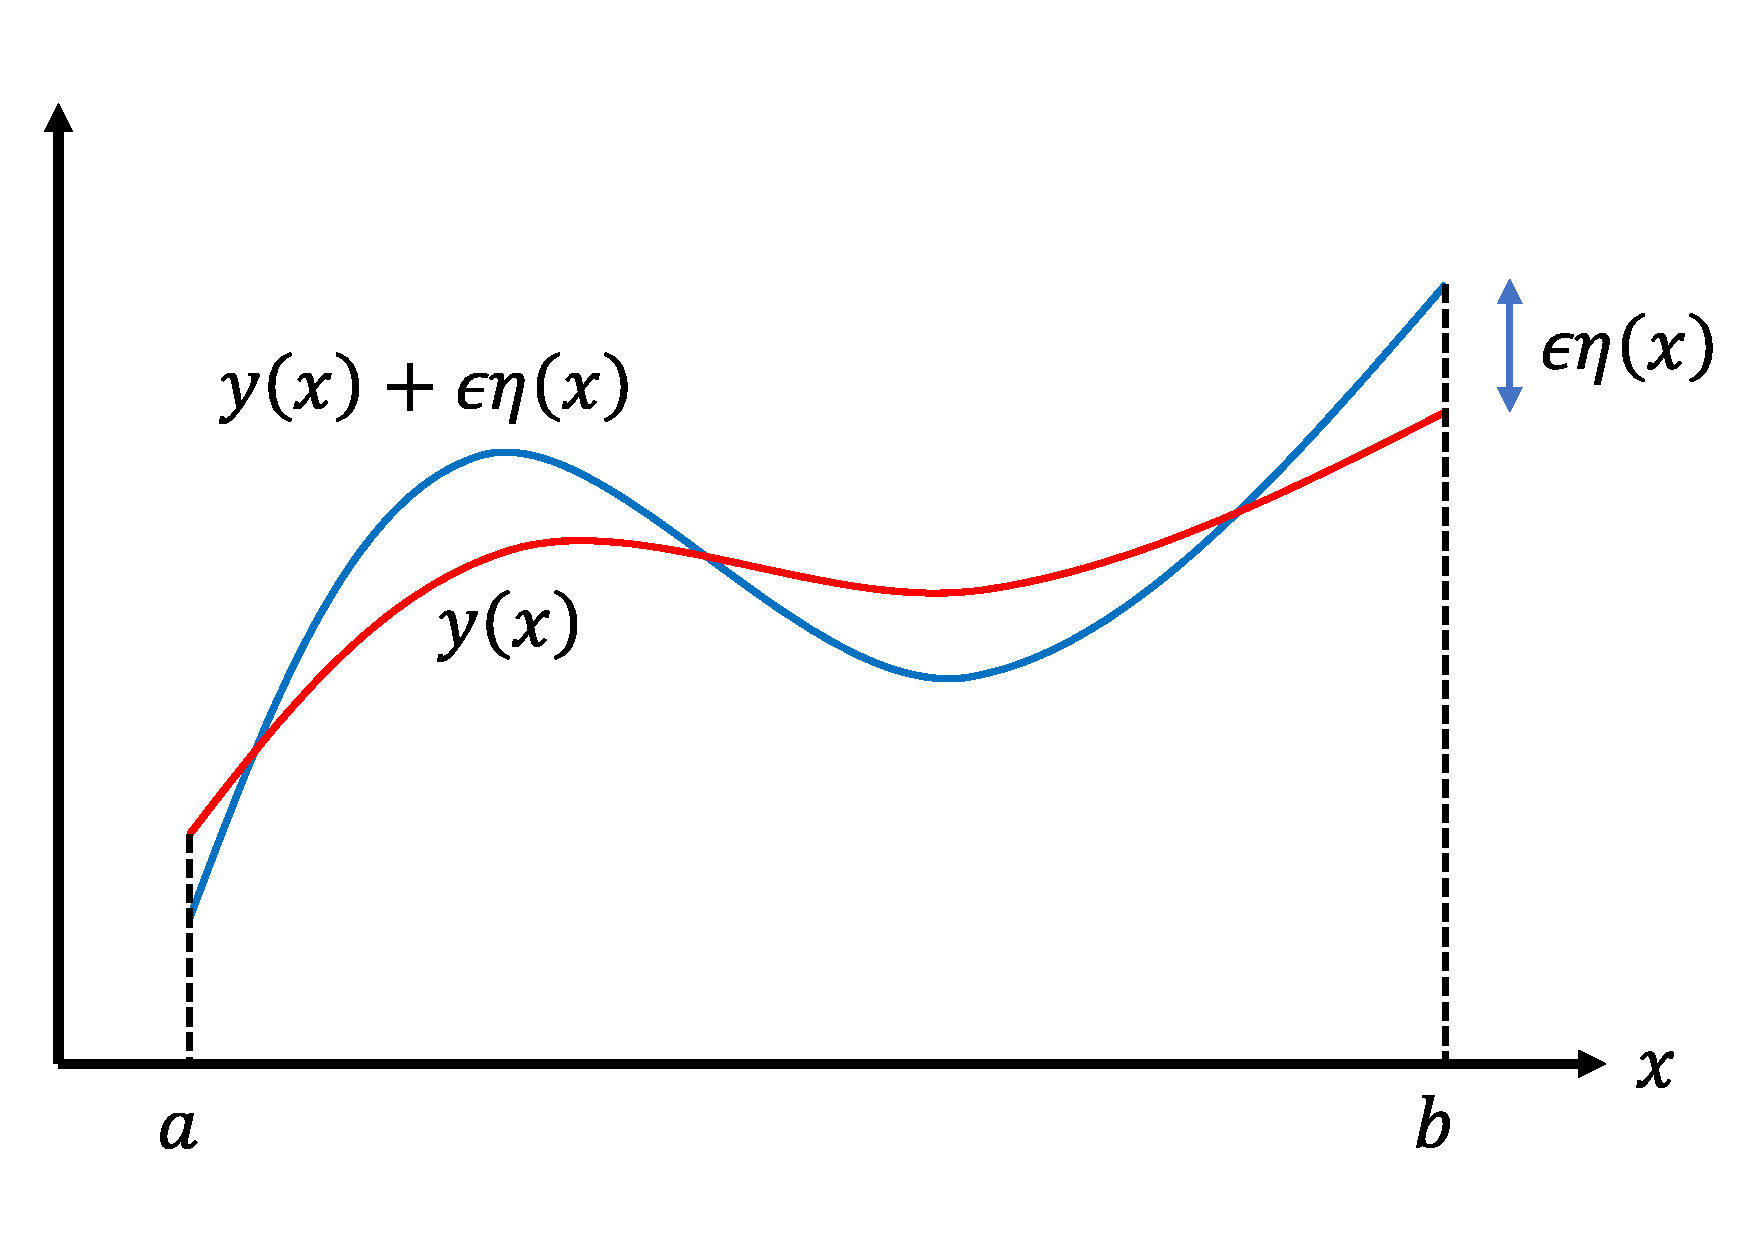
\includegraphics[scale=0.28]{functional-derivative.pdf}
	\caption{区間$[a, b]$で定義された関数$y(x)$の表現}
	\label{fig:function-derivative-example}
\end{figure}

\end{frame}

\begin{frame}{変分法}

\begin{itemize}
	\item 汎関数の最適化
	\begin{itemize}
		\item 汎関数$F[y]$が最大(最小)となるとき、\color{red}関数$y(x)$の微小な変化に対して、汎関数は変化しないはず\normalcolor
		\item 即ち、汎関数が最大(最小)となるとき、$F[y(x) + \epsilon \eta(x)] = F[y(x)]$が成り立つ
		\item 従って、変分の定義式から、以下が成り立つ
		\begin{equation}
			\int_a^b \frac{\delta F}{\delta y(x)} \eta(x) dx = 0
		\end{equation}
		
		\item 上式は任意の$\eta(x)$について成立しなければならない
		\item 従って、変分$\delta F/\delta y$は、任意の$x$について$0$とならなければならない
		\newline
		\item 汎関数$F[y]$が最大(最小)となるとき、\color{red}$\delta F/\delta y = 0$\normalcolor が成立することが分かった (\alert{通常の微分と同じ})
	\end{itemize}
\end{itemize}

\end{frame}

\begin{frame}{変分法}

\begin{itemize}
	\item 変分法の例
	\begin{itemize}
		\item 様々な汎関数について、変分を導出してみよう
		\item また、その汎関数が最大(最小)となるときに成り立つ条件を、導出してみよう
	\end{itemize}
\end{itemize}

\end{frame}

\begin{frame}{変分法}
	
\begin{itemize}
	\item 汎関数の例(1)
	\begin{itemize}
		\item $y(x)$とその微分$y'(x) = dy/dx$、そして$x$によって決まる関数\color{red}$G(y(x), y'(x), x)$\normalcolor があるとする
		\newline
		\item 汎関数$F[y]$を、$G(y(x), y'(x), x)$を区間$[a, b]$にわたって積分した結果を出力する関数として、次のように定める
		\begin{equation}
			F[y] = \int_a^b G(y(x), y'(x), x) dx
		\end{equation}
		
		\item 積分区間は無限であってもよいとする($a = -\infty, b = \infty$でもよい)
		\newline
		\item $y(x)$に摂動$\epsilon \eta(x)$を加えたときの、汎関数の値$F[y(x) + \epsilon \eta(x)]$を使って、変分$\delta F/\delta y$を調べてみる
		\begin{equation}
			F[y(x) + \epsilon \eta(x)] = \int_a^b G(y(x) + \epsilon \eta(x), y'(x) + \epsilon \eta'(x), x) dx
		\end{equation}
		ここで、被積分項のテーラー展開を考えれば
		\begin{eqnarray}
			&& G(y(x) + \epsilon \eta(x), y'(x) + \epsilon \eta'(x), x) \nonumber \\
			&=& G(y(x), y'(x), x) + \frac{\partial G}{\partial y} \epsilon \eta(x) + \nonumber \\
			&& \qquad \frac{\partial G}{\partial y'} \epsilon \eta'(x) + \frac{\partial G}{\partial x} \cdot 0 + O(\epsilon^2) \\
			&=& G(y(x), y'(x), x) + \epsilon \left( \frac{\partial G}{\partial y} \eta(x) + \frac{\partial G}{\partial y'} \eta'(x) \right) + O(\epsilon^2)
		\end{eqnarray}
		であるから
		\begin{eqnarray}
			&& F[y(x) + \epsilon \eta(x)] \nonumber \\
			&=& \int_a^b G(y(x) + \epsilon \eta(x), y'(x) + \epsilon \eta'(x), x) dx \nonumber \\
			&=& \int_a^b \bigg( G(y(x), y'(x), x) + \nonumber \\
			&& \qquad \left. \epsilon \left( \frac{\partial G}{\partial y} \eta(x) + \frac{\partial G}{\partial y'} \eta'(x) \right) + O(\epsilon^2) \right) dx \\
			&=& \int_a^b G(y(x), y'(x), x) dx + \nonumber \\
			&& \qquad \epsilon \int_a^b \left( \frac{\partial G}{\partial y} \eta(x) + \frac{\partial G}{\partial y'} \eta'(x) \right) dx + O(\epsilon^2) \\
			&=& F[y(x)] + \epsilon \int_a^b \left( \frac{\partial G}{\partial y} \eta(x) + \frac{\partial G}{\partial y'} \eta'(x) \right) dx + O(\epsilon^2)
		\end{eqnarray}
		ここで
		\begin{eqnarray}
			&& \int_a^b \left( \frac{\partial G}{\partial y} \eta(x) + \frac{\partial G}{\partial y'} \eta'(x) \right) dx \nonumber \\
			&=& \int_a^b \left( \frac{\partial G}{\partial y} \eta(x) \right) dx + \int_a^b \left( \frac{\partial G}{\partial y'} \eta'(x) \right) dx \\
			&=& \int_a^b \left( \frac{\partial G}{\partial y} \eta(x) \right) dx + \nonumber \\
			&& \qquad \left[ \frac{\partial G}{\partial y'} \eta(x) \right]_a^b - \int_a^b \frac{d}{dx} \left( \frac{\partial G}{\partial y'} \right) \eta(x) dx \\
			&=& \left[ \frac{\partial G}{\partial y'} \eta(x) \right]_a^b + \int_a^b \left( \frac{\partial G}{\partial y} - \frac{d}{dx} \left( \frac{\partial G}{\partial y'} \right) \right) \eta(x) dx
		\end{eqnarray}
		である
		\newline
		\item 途中の式変形では、部分積分を使っていることに注意
		\newline
		\item いま、積分区間の両端において、$y(x)$の値は固定されているとする
		\item これを\alert{固定端条件}という (図\ref{fig:function-derivative-example-2})
		\newline
		\item このとき、$\eta(a) = \eta(b) = 0$であるから、上式の最初の項が消えて
		\begin{eqnarray}
			&& \int_a^b \left( \frac{\partial G}{\partial y} \eta(x) + \frac{\partial G}{\partial y'} \eta'(x) \right) dx \nonumber \\
			&=& \left[ \frac{\partial G}{\partial y'} \eta(x) \right]_a^b + \int_a^b \left( \frac{\partial G}{\partial y} - \frac{d}{dx} \left( \frac{\partial G}{\partial y'} \right) \right) \eta(x) dx \\
			&=& \int_a^b \left( \frac{\partial G}{\partial y} - \frac{d}{dx} \left( \frac{\partial G}{\partial y'} \right) \right) \eta(x) dx
		\end{eqnarray}
		のようになる
		
		\item 従って、摂動を加えたときの汎関数の値$F[y(x) + \epsilon \eta(x)]$は
		\begin{eqnarray}
			&& F[y(x) + \epsilon \eta(x)] \nonumber \\
			&=& F[y(x)] + \epsilon \int_a^b \left( \frac{\partial G}{\partial y} - \frac{d}{dx} \left( \frac{\partial G}{\partial y'} \right) \right) \eta(x) dx + O(\epsilon^2)
		\end{eqnarray}
		となる
		\newline
		
		\item 上式を、変分の定義式と比べれば
		\begin{equation}
			F[y(x) + \epsilon \eta(x)] = F[y(x)] + \epsilon \int_a^b \frac{\delta F}{\delta y(x)} \eta(x) dx + O(\epsilon^2)
		\end{equation}
		変分$\delta F/\delta y$は次のように書ける
		\begin{equation}
			\color{red}\frac{\delta F}{\delta y(x)} = \frac{\partial G}{\partial y} - \frac{d}{dx} \left( \frac{\partial G}{\partial y'} \right)\normalcolor
		\end{equation}
		
		\item 汎関数$F[y]$が最大(最小)になるとき、変分$\delta F/\delta y$が$0$になる
		\item 従って、汎関数が最大(最小)になるとき、以下の方程式が成り立つ
		\begin{equation}
			\frac{\partial G}{\partial y} - \frac{d}{dx} \left( \frac{\partial G}{\partial y'} \right) = 0
		\end{equation}
		
		\item これを\alert{オイラー-ラグランジュ方程式}という
		\newline
		
		\item オイラー-ラグランジュ方程式は、次のような考え方で導出することもできる
		\newline
		\item $F[y]$が最大(最小)であれば、摂動$\epsilon \eta(x)$によって$y(x)$が少し変化しても、$F[y]$の値は変化しないはず
		\item 従って、$F[y]$が最大(最小)であるとき、\color{red}$F[y]$の$\epsilon$による微分は$0$になるはず\normalcolor
		
		\item これを数式で表現すると、次のようになる
		\begin{equation}
			\left. \frac{\partial F[y]}{\partial \epsilon} \right|_{\epsilon = 0} = 0
		\end{equation}
		左辺は通常の偏微分であり、これを計算すると
		\begin{eqnarray}
			&& \frac{\partial F[y]}{\partial \epsilon} \nonumber \\
			&=& \frac{\partial}{\partial \epsilon} \int_a^b G(y, y', x) dx \\
			&=& \int_a^b \frac{\partial}{\partial \epsilon} G(y, y', x) dx \\
			&=& \int_a^b \left( \frac{\partial G}{\partial y} \frac{\partial y}{\partial \epsilon} + \frac{\partial G}{\partial y'} \frac{\partial y'}{\partial \epsilon} + \frac{\partial G}{\partial x} \frac{\partial x}{\partial \epsilon} \right) dx \\
			&=& \int_a^b \left( \frac{\partial G}{\partial y} \eta(x) + \frac{\partial G}{\partial y'} \eta'(x) \right) dx \\
			&=& \left[ \frac{\partial G}{\partial y'} \eta(x) \right]_a^b + \int_a^b \left( \frac{\partial G}{\partial y} - \frac{d}{dx} \left( \frac{\partial G}{\partial y'} \right) \right) \eta(x) dx \\
			&& \qquad (\because \eta(a) = \eta(b) = 0) \nonumber \\
			&=& \int_a^b \left( \frac{\partial G}{\partial y} - \frac{d}{dx} \left( \frac{\partial G}{\partial y'} \right) \right) \eta(x) dx \\
			&=& 0 \nonumber
		\end{eqnarray}
		
		\item 上の式変形では、$y = y(x) + \epsilon \eta(x)$であるから
		\begin{eqnarray}
			&& \frac{\partial y}{\partial \epsilon} = \eta(x) \\
			&& \frac{\partial y'}{\partial \epsilon} = \frac{\partial}{\partial \epsilon} \left( \frac{\partial y}{\partial x} \right) = \frac{\partial}{\partial \epsilon} \left( y'(x) + \epsilon \eta'(x) \right) = \eta'(x) \\
			&& \frac{\partial x}{\partial \epsilon} = 0
		\end{eqnarray}
		が成立することを利用している
		\newline
		
		\item 任意の$\eta(x)$について、上式が恒等的に成り立つためには
		\begin{equation}
			\frac{\partial G}{\partial y} - \frac{d}{dx} \left( \frac{\partial G}{\partial y'} \right) = 0
		\end{equation}
		でなければならないことが分かり、先程と同様に、オイラー-ラグランジュ方程式を得る
	\end{itemize}
\end{itemize}

\end{frame}

\begin{frame}{変分法}

\begin{figure}[h]
	\centering
	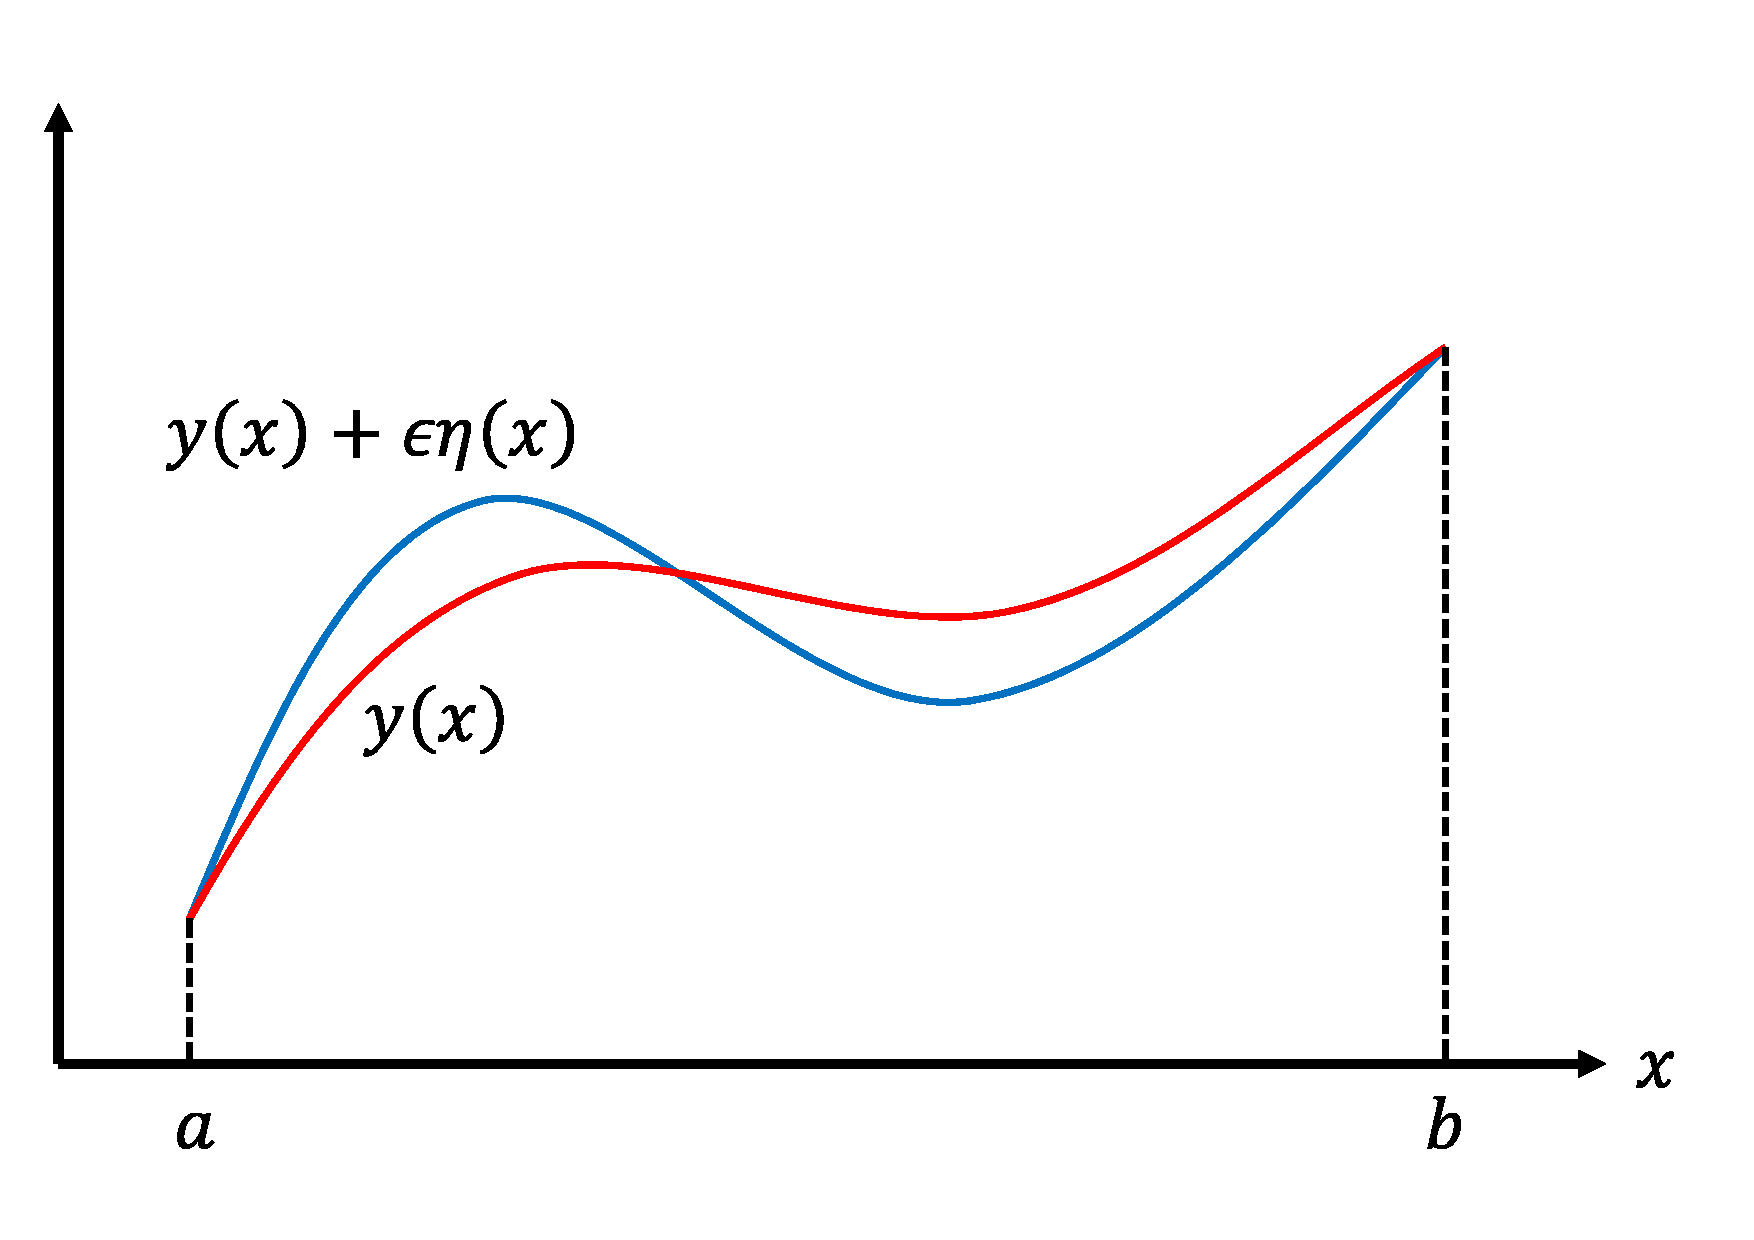
\includegraphics[scale=0.28]{functional-derivative-2.pdf}
	\caption{制約条件を含んでいる場合の表現}
	\label{fig:function-derivative-example-2}
\end{figure}

\end{frame}

\begin{frame}{変分法}

\begin{itemize}
	\item 汎関数の例(2)
	\begin{itemize}
		\item 上では$G(y(x), y'(x), x)$について考えて、変分を導出した
		\item $y(x)$と$x$のみによって決まり、$y'(x)$には依存しない関数\color{red}$G(y(x), x)$\normalcolor を考えよう
		\newline
		\item 汎関数$F[y]$は、先程と同様に以下で表されるとする
		\begin{equation}
			F[y] = \int_a^b G(y(x), x) dx
		\end{equation}
		
		\item このとき変分$\delta F/\delta y$を求めるのは、非常に簡単である
		\item 先程の式に、$\partial G/\partial y' = 0$を代入すれば直ちに得られる
		\begin{equation}
			\color{red}\frac{\delta F}{\delta y(x)} = \frac{\partial G}{\partial y}\normalcolor
		\end{equation}
		
		\item あるいは以下のように書ける
		\begin{equation}
			\color{red}\frac{\delta}{\delta y(x)} \int_a^b G(y(x), x) dx = \frac{\partial}{\partial y} G(y(x), x)\normalcolor
		\end{equation}
		
		\item $F[y]$が最大(最小)であるとき、以下のオイラー-ラグランジュ方程式が成り立つ
		\begin{equation}
			\frac{\partial G}{\partial y} = 0
		\end{equation}
	\end{itemize}
\end{itemize}

\end{frame}

\begin{frame}{変分法}

\begin{itemize}
	\item 汎関数の例(3)
	\begin{itemize}
		\item 今度は、$y'(x)$と$x$のみによって決まり、$y(x)$には依存しない関数\color{red}$G(y'(x), x)$\normalcolor を考えよう
		\newline
		\item この場合も変分$\delta F/\delta y$を求めるのは簡単である
		\item $G(y(x), y'(x), x)$の変分の式に、$\partial G/\partial y = 0$を代入すればよい
		\begin{equation}
			\color{red}\frac{\delta F}{\delta y(x)} = - \frac{d}{dx} \left( \frac{\partial G}{\partial y'} \right)
		\end{equation}
		
		\item オイラー-ラグランジュ方程式は次のようになる
		\begin{equation}
			- \frac{d}{dx} \left( \frac{\partial G}{\partial y'} \right) = 0
		\end{equation}
	\end{itemize}
\end{itemize}

\end{frame}

\begin{frame}{変分法}

\begin{itemize}
	\item 汎関数の例(4)
	\begin{itemize}
		\item $y(x)$と$y'(x)$によって決まる関数\color{red}$G(y(x), y'(x))$\normalcolor を考えよう
		\item このときのオイラー-ラグランジュ方程式を導出してみよう
		\newline
		\item $G(y(x), y'(x))$を$x$で微分すれば
		\begin{eqnarray}
			&& \frac{d}{dx} G(y, y') \nonumber \\
			&=& \frac{\partial}{\partial y} G(y, y') \frac{dy}{dx} + \frac{\partial}{\partial y'} G(y, y') \frac{dy'}{dx} \\
			&=& y' \frac{\partial}{\partial y} G(y, y') + \frac{\partial}{\partial y'} G(y, y') \frac{dy'}{dx}
		\end{eqnarray}
		となるから
		\begin{equation}
			y' \frac{\partial}{\partial y} G(y, y') = \frac{d}{dx} G(y, y') - \frac{\partial}{\partial y'} G(y, y') \frac{dy'}{dx}
		\end{equation}
		また、オイラー-ラグランジュ方程式の両辺に$y'$を掛けたものは
		\begin{equation}
			y' \frac{\partial}{\partial y} G(y, y') - y' \frac{d}{dx} \left( \frac{\partial}{\partial y'} G(y, y') \right) = 0
		\end{equation}
		これらを連立させて
		\begin{eqnarray}
			&& y' \frac{d}{dx} \left( \frac{\partial}{\partial y'} G(y, y') \right) = \frac{d}{dx} G(y, y') - \frac{\partial}{\partial y'} G(y, y') \frac{dy'}{dx} \\
			&& y' \frac{d}{dx} \left( \frac{\partial}{\partial y'} G(y, y') \right) + \frac{\partial}{\partial y'} G(y, y') \frac{dy'}{dx} = \frac{d}{dx} G(y, y') \\
			&& \frac{d}{dx} \left( y' \cdot \frac{\partial}{\partial y'} G(y, y') \right) = \frac{d}{dx} G(y, y') \\
			&& \int \left( \frac{d}{dx} \left( y' \cdot \frac{\partial}{\partial y'} G(y, y') \right) \right) dx = \nonumber \\
			&& \qquad \int \left( \frac{d}{dx} G(y, y') \right) dx + C \\
			&& G(y, y') = y' \cdot \frac{\partial}{\partial y'} G(y, y') + C
		\end{eqnarray}
		となるので、結局オイラー-ラグランジュ方程式は
		\begin{equation}
			G - y' \frac{\partial G}{\partial y'} = \mathrm{Const.}
		\end{equation}
		と書ける
	\end{itemize}
\end{itemize}

\end{frame}

\subsection{変分法で解ける問題の例}

\begin{frame}{変分法で解ける問題の例}

\begin{itemize}
	\item 変分法で解ける問題の例(1)
	\begin{itemize}
		\item 2点$P(0, 0)$、$Q(a, b)$を結ぶ最短経路は?
		\newline
		\item 2点を結ぶ経路$y = f(x)$($0 \le x \le a$)の長さ$l$は、次のようになる
		\begin{equation}
			l = \int_0^a \sqrt{1 + \left( \frac{dy}{dx} \right)^2} dx = \int_0^a \sqrt{1 + y'^2} dx
		\end{equation}
		
		\item 被積分項が$y'$のみの関数となっていることが分かる
		\item $G(y'(x), x)$の場合の公式を使えば、$l$の$y = f(x)$による変分が求まる
		\begin{eqnarray}
			\frac{\delta l}{\delta f(x)} &=& - \frac{d}{dx} \left( \frac{\partial}{\partial y'} \sqrt{1 + y'^2} \right) \\
			&=& - \frac{d}{dx} \left( \frac{1}{2} \frac{1}{\sqrt{1 + y'^2}} \frac{\partial}{\partial y'} \left( 1 + y'^2 \right) \right) \\
			&=& - \frac{d}{dx} \frac{y'}{\sqrt{1 + y'^2}}
		\end{eqnarray}
		
		\item $l$を最小化するような$y = f(x)$は、上式の変分を$0$と等置すれば
		\begin{eqnarray}
			&& - \frac{d}{dx} \frac{y'}{\sqrt{1 + y'^2}} = 0 \\
			&\therefore& \frac{y'}{\sqrt{1 + y'^2}} = \mathrm{Const.}
		\end{eqnarray}
		
		\item これは、\color{red}$y'$が定数である\normalcolor ことを意味している
		\item 従って、\color{red}$y = C_0 x + C_1$\normalcolor と書ける
		\newline
		\item 以上より、\color{red}2点間を結ぶ最短経路は直線\normalcolor である
		\newline
		\item $y = f(x)$の形について、\alert{具体的な仮定は特に置いていない}ことに注意
		\item 変分法では、\alert{関数そのものを最適化する}
		\item 従って、関数の具体的な形については、特に仮定する必要がない
	\end{itemize}
\end{itemize}

\end{frame}

\begin{frame}{変分法で解ける問題の例}

\begin{itemize}
	\item 変分法で解ける問題の例(2)
	\begin{itemize}
		\item エントロピーが最大になるような確率分布は?
		\newline
		
		\item 確率変数が離散的である場合は、一様分布(変数の取り得る状態が等確率であるとき)
		\item それでは、\alert{連続変数の場合}はどのようになるか?
		\newline
		\item 確率分布$p(x)$のエントロピー$H[p]$は次で定義された
		\begin{equation}
			H[p] = -\int p(x) \ln p(x) dx
		\end{equation}
		
		\item $H[p]$を単純に最大化するだけでは、$p$は確率分布とはならない可能性がある
		\item そこで、\color{red}$p(x)$の$x$による積分が$1$になる\normalcolor という制約を付けた最大化を行う
		\newline
		\item 分散が増加するにつれて、エントロピーは無限に増加する
		\item これでは、どの分布が最大のエントロピーを持つかという問題を考える意味がなくなってしまう
		\item そこで、\color{red}分布の分散を$\sigma^2$に固定\normalcolor したうえで、最大のエントロピーを持つものを探す
		\newline
		\item 分布を$x$方向にずらせば、エントロピーを変更せずに分布を任意に変化させられてしまう
		\item これより、解が無限に存在するため、劣決定系となってしまう
		\item そこで、\color{red}分布の平均を$\mu$に固定\normalcolor して、解が唯一に定まるようにする
		\newline
		\item 即ち、以下の3つの制約の下で、ラグランジュの未定乗数法を使って、エントロピー$H[p]$を最大化する
		\begin{eqnarray}
			\int p(x) dx &=& 1 \\
			\int x p(x) dx &=& \mu \\
			\int (x - \mu)^2 p(x) dx &=& \sigma^2
		\end{eqnarray}
		
		\item 最大化すべきラグランジュ汎関数$\mathcal{L}[p]$は次のようになる
		\begin{eqnarray}
			&& \mathcal{L}[p] \nonumber \\
			&=& -\int p(x) \ln p(x) dx + \lambda_1 \left( \int p(x) dx - 1 \right) + \nonumber \\
			&& \qquad \lambda_2 \left( \int x p(x) dx - \mu \right) + \nonumber \\
			&& \qquad \lambda_3 \left( \int (x - \mu)^2 p(x) dx - \sigma^2 \right) \\
			&=& \int \left( \lambda_1 p(x) + \lambda_2 x p(x) + \lambda_3 (x - \mu)^2 p(x) - p(x) \ln p(x) \right) dx - \nonumber \\
			&& \qquad \lambda_1 - \mu \lambda_2 - \sigma^2 \lambda_3
		\end{eqnarray}
		
		\item $\mathcal{L}[p]$を$p(x)$について変分最適化する
		\begin{eqnarray}
			&& \frac{\delta}{\delta p(x)} \mathcal{L}[p] \nonumber \\
			&=& \frac{\delta}{\delta p(x)} \int \left( \lambda_1 p(x) + \lambda_2 x p(x) + \lambda_3 (x - \mu)^2 p(x) - p(x) \ln p(x) \right) dx \nonumber \\
			&=& \frac{\partial}{\partial p(x)} \left( \lambda_1 p(x) + \lambda_2 x p(x) + \lambda_3 (x - \mu)^2 p(x) - p(x) \ln p(x) \right) \nonumber \\
			&=& \lambda_1 + \lambda_2 x + \lambda_3 (x - \mu)^2 - \ln p(x) - 1 = 0
		\end{eqnarray}
		
		\item これより以下を得るので、$p(x)$は\alert{ガウス分布}であると分かる
		\begin{equation}
			p(x) = \exp \left( -1 + \lambda_1 + \lambda_2 x + \lambda_3 (x - \mu)^2 \right)
		\end{equation}
		
		\item ラグランジュ乗数$\lambda_1, \lambda_2, \lambda_3$は次のようにすれば、3つの制約が満たされる
		\begin{eqnarray}
			\lambda_1 &=& 1 - \ln \left( 2 \pi \sigma^2 \right) \\
			\lambda_2 &=& 0 \\
			\lambda_3 &=& \frac{1}{2 \sigma^2}
		\end{eqnarray}
		
		\item これより、$p(x)$は次のように書ける
		\begin{eqnarray}
			p(x) &=& \exp \left( -1 + 1 - \ln \left( 2 \pi \sigma^2 \right) + \frac{1}{2 \sigma^2} (x - \mu)^2 \right) \nonumber \\
			&=& \exp \left( - \ln \left( 2 \pi \sigma^2 \right) \right) \exp \left( \frac{1}{2 \sigma^2} (x - \mu)^2 \right) \nonumber \\
			&=& \frac{1}{2 \pi \sigma^2} \exp \left( \frac{1}{2 \sigma^2} (x - \mu)^2 \right) \\
			&=& \mathcal{N}(x | \mu, \sigma^2)
		\end{eqnarray}
		
		\item エントロピーを最大化する分布は、ガウス分布であることが分かった
		\newline
		
		\item エントロピーを最大化する際に、分布が非負になるという制約は置かなかった
		\item しかし、結果として得られた分布は非負であるから、制約をラグランジュ乗数で取り込む必要はなかった
	\end{itemize} \
	
	\item エントロピーを最小化するような分布は?
	\begin{itemize}
		\item エントロピーを最小化する特定の分布は存在しない
		\newline
		\item 2つの点$x = \mu + \sigma, \mu - \sigma$に多くの確率密度を配置し、他の全ての$x$について、より少ない確率密度を配置することで、分散$\sigma^2$を維持したままエントロピーを小さくできる
		\newline
		\item これを続けると、2点$x = \mu + \sigma, \mu - \sigma$に無限の確率密度をもち、他の全ての$x$について、確率密度が$0$となるように、収束していく
		\item この極限では、2つのデルタ関数の足し合わせ(混合ディラック分布)となる
		\item これは、単一の確率分布関数では記述できない
		\item 従って、上記のように、汎関数微分が$0$となる特定の関数について解く手法では、得られない解である
	\end{itemize}
\end{itemize}

\end{frame}

\subsection{変分法のまとめ}

\begin{frame}{変分法のまとめ}

\begin{itemize}
	\item 変分のまとめ
	\begin{itemize}
		\item これまでの計算で、次の変分が明らかとなった
		\begin{eqnarray}
			&& \frac{\delta}{\delta y(x)} \int G(y(x), y'(x), x) dx = \nonumber \\
			&& \qquad \frac{\partial}{\partial y} G(y(x), y'(x), x) - \frac{d}{dx} \left( \frac{\partial}{\partial y'} G(y(x), y'(x), x) \right) \\
			&& \frac{\delta}{\delta y(x)} \int G(y(x), x) dx = \frac{\partial}{\partial y} G(y(x), x) \\
			&& \frac{\delta}{\delta y(x)} \int G(y'(x), x) dx = - \frac{d}{dx} \left( \frac{\partial}{\partial y'} G(y'(x), x) \right)
		\end{eqnarray}
	\end{itemize}
\end{itemize}

\end{frame}

\begin{frame}{変分法のまとめ}

\begin{itemize}
	\item ここまでの話の流れ
	\begin{enumerate}
		\item 変分の定義や、変分の計算法について調査した
		\newline
		\item \alert{変分}(汎関数の微分)とは、入力関数が微小に変化したときの、出力値の変化量として定義される
		\newline
		\item 汎関数が特定の形で表せるとき、変分がどのようになるか計算した
		\item 汎関数が最大(最小)になるとき、\alert{オイラー-ラグランジュ方程式}が成立した
		\newline
		\item 変分法を用いて、2点間を結ぶ最短経路が\alert{直線}になることを確認した
	\end{enumerate} \
	
	\item これからの話の流れ
	\begin{itemize}
		\item 変分最適化を、どのように推論問題に適用するのかについて調べていく
	\end{itemize}
\end{itemize}

\end{frame}

\end{document}


% approximate-inference.tex

\documentclass[dvipdfmx,notheorems,t]{beamer}

\usepackage{docmute}

% settings.tex

\AtBeginDvi{\special{pdf:tounicode 90ms-RKSJ-UCS2}}

\AtBeginSection[]{\frame[t]{\frametitle{目次}
	\tableofcontents[currentsection,hideallsubsections]}}

\AtBeginSubsection[]{\frame[t]{\frametitle{目次}
	\tableofcontents[currentsection,currentsubsection,subsectionstyle=show/shaded/hide]}}

\usefonttheme{professionalfonts}
\usetheme{Madrid}

\setbeamercovered{transparent=30} 
% \setbeamertemplate{navigation symbols}{}
\setbeamertemplate{frametitle}[default][left]
\setbeamertemplate{frametitle continuation}{}
\setbeamertemplate{enumerate items}[square]
\setbeamertemplate{caption}[numbered]

\let\oldframe\frame
\renewcommand\frame[1][allowdisplaybreaks,allowframebreaks,t]{\oldframe[#1]}

\usepackage{bxdpx-beamer}
\usepackage{pxjahyper}
\usepackage{minijs}

\usepackage{amsmath}
\usepackage{amssymb}
\usepackage{amsthm}
\usepackage{bm}

\DeclareMathOperator*{\argmax}{arg\,max}
\DeclareMathOperator*{\argmin}{arg\,min}
\DeclareMathOperator{\Tr}{Tr}
\DeclareMathOperator{\KL}{KL}
\DeclareMathOperator{\diag}{diag}

\usepackage[T1]{fontenc}
\usepackage[utf8]{inputenc}

\setbeamertemplate{theorems}[numbered]
\theoremstyle{definition}
\newtheorem{theorem}{定理}
\newtheorem{definition}{定義}
\newtheorem{proposition}{命題}
\newtheorem{lemma}{補題}
\newtheorem{corollary}{系}
\newtheorem{conjecture}{予想}
\newtheorem*{remark}{Remark}
\renewcommand{\proofname}{}

\renewcommand{\figurename}{図}
\renewcommand{\tablename}{表}

\renewcommand{\kanjifamilydefault}{\gtdefault}


\begin{document}

\section{近似推論法}

\subsection{変分推論}

\begin{frame}{変分推論}

\begin{itemize}
	\item 変分推論が必要だった理由
	\begin{itemize}
		\item 潜在変数に関する事後分布$p(\bm{Z} | \bm{X}, \bm{\theta})$の計算は、困難であることが多い
		\item どのような場合に困難になるのか、次の図\ref{fig:example-of-inference-problems}に示す
		\newline
		\item $p(\bm{Z} | \bm{X}, \bm{\theta})$の厳密な計算は諦める代わりに、\alert{別の確率分布で近似}したい
		\newline
		\item 別の確率分布で近似するとき、単純な項の積として表現できるといった、\alert{何らかの仮定を置く}
	\end{itemize}
\end{itemize}

\end{frame}

\begin{frame}{変分推論}

\begin{figure}[h]
	\centering
	\includegraphics[clip,scale=0.6,trim=2cm 17.8cm 2cm 5cm,page=647]{../goodfellow-deep-learning.pdf}
	\caption{事後分布$p(\bm{Z} | \bm{X})$の計算が困難な場合}
	\label{fig:example-of-inference-problems}
\end{figure}

\end{frame}

\begin{frame}{変分推論}

\begin{figure}[h]
	\centering
	\includegraphics[clip,scale=0.6,trim=2cm 10cm 2cm 11.8cm,page=647]{../goodfellow-deep-learning.pdf}
	\caption{事後分布$p(\bm{Z} | \bm{X})$の計算が困難な場合}
	\label{fig:example-of-inference-problems-2}
\end{figure}

\end{frame}

\begin{frame}{変分推論}

\begin{itemize}
	\item 事後分布$p(\bm{Z} | \bm{X})$の計算が困難な場合1
	\begin{itemize}
		\item グラフィカルモデルにおいて、\alert{潜在変数間の相互作用がある}場合、計算が困難になる
		\newline
		\item 左側の\alert{半制限付きボルツマンマシン}では、全ての潜在変数の組み合わせ間で、接続がある
		\item 従って、潜在変数間に\alert{依存関係}が存在し、事後分布の計算が手に負えない
		\newline
		\item 白丸で描かれた潜在変数を$\bm{Z} = \left\{ z_1, z_2, z_3 \right\}$、灰色で描かれた観測データを$\bm{X}$とおくと、事後分布$p(\bm{Z} | \bm{X})$は、例えば次のようになる
		\begin{eqnarray}
			&& p(z_1, z_2, z_3 | \bm{X}) \nonumber \\
			&=& p(z_1 | \bm{X}, z_2, z_3) p(z_2 | \bm{X}, z_3) p(z_3 | \bm{X})
		\end{eqnarray}
	\end{itemize} \
	
	\item 事後分布$p(\bm{Z} | \bm{X})$の計算が困難な場合2
	\begin{itemize}
		\item 中央は、層間の結合がない潜在変数の層で構成される、\alert{深層ボルツマンマシン}を表す
		\item 潜在変数の層間の結合があるため、事後分布の計算が手に負えない
		\newline
		\item 上の層の潜在変数を$\bm{Z}_1 = \left\{ z_{11}, z_{12}, z_{13} \right\}$、中間層の潜在変数を$\bm{Z}_2 = \left\{ z_{21}, z_{22}, z_{23} \right\}$、灰色で描かれた観測データを$\bm{X}$とおくと、事後分布は、例えば次のようになる
		\begin{eqnarray}
			&& p(\bm{Z}_1, \bm{Z}_2 | \bm{X}) \nonumber \\
			&=& p(\bm{Z}_2 | \bm{X}) p(\bm{Z}_1 | \bm{Z}_2) \\
			&=& p(z_{21}, z_{22}, z_{23} | \bm{X}) p(z_{11}, z_{12}, z_{13} | \bm{Z}_2) \nonumber \\
			&=& p(z_{21} | \bm{X}) p(z_{22} | \bm{X}) p(z_{23} | \bm{X}) \nonumber \\
			&& \qquad p(z_{11} | \bm{Z}_2) p(z_{12} | \bm{Z}_2) p(z_{13} | \bm{Z}_2)
		\end{eqnarray}
	\end{itemize}
\end{itemize}

\end{frame}

\subsection{座標降下法}

\begin{frame}{変分推論}

\begin{itemize}
	\item 変分推論の目的
	\begin{itemize}
		\item 同時分布$p(\bm{X}, \bm{Z})$が求まっているときに、\alert{事後分布}$p(\bm{Z} | \bm{X})$と、\alert{エビデンス}$p(\bm{X})$の近似を求める
	\end{itemize} \
	
	\item 注意点
	\begin{itemize}
		\item 観測変数と潜在変数をそれぞれ、$\bm{X}, \bm{Z}$とおく
		\item $p(\bm{X})$は、確率モデルからデータ$\bm{X}$が生起する確率である
		\item \alert{データからみたモデルの好み}と解釈できるから、$p(\bm{X})$を\alert{モデルエビデンス}という
	\end{itemize}
\end{itemize}

\end{frame}

\begin{frame}{変分推論}

\begin{itemize}
	\item 周辺分布の対数$\ln p(\bm{X})$の分解
	\begin{itemize}
		\item EMアルゴリズムのときと同様であり、次のように分解できる
		\begin{equation}
			\ln p(\bm{X}) = \mathcal{L}(q) + \KL (q || p)
		\end{equation}
		
		\item 但し、$\mathcal{L}(q)$と$\KL (q || p)$は次のように定義した
		\begin{eqnarray}
			\mathcal{L}(q) &=& \int q(\bm{Z}) \ln \frac{p(\bm{X}, \bm{Z})}{q(\bm{Z})} d\bm{Z} \\
			\KL (q || p) &=& -\int q(\bm{Z}) \ln \frac{p(\bm{Z} | \bm{X})}{q(\bm{Z})} d\bm{Z}
		\end{eqnarray}
	\end{itemize} \
		
	\item パラメータ$\bm{\theta}$の扱い
	\begin{itemize}
		\item EMアルゴリズムとは異なり、\color{red}パラメータ$\bm{\theta}$がどこにも現れていない\normalcolor
		% \item ここでは、全てのパラメータに事前分布が与えられた、\alert{完全にベイズ的なモデル}を考えている
		% \item パラメータも、確率変数として$\bm{Z}$の中に含まれている
		\item \alert{パラメータも潜在変数として扱っている}ので、パラメータベクトルは明示的には書かない
		\item ここでは、パラメータ$\bm{\theta}$については、あまり気にしない
		\newline
		\item ここでは連続潜在変数について考えるが、離散潜在変数であれば、積分を$\bm{Z}$に関する総和に置き換えればよい
	\end{itemize} \
	
	\item 下界$\mathcal{L}(q)$を最適化する動機
	\begin{itemize}
		\item $\mathcal{L}(q)$はエビデンスの対数$\ln p(\bm{X})$の下界であるから、\alert{エビデンス下界}(Evidence lower bound, \alert{ELBO})ともいう
		\item または、負の\alert{変分自由エネルギー}(Variational free energy)という
		\newline
		
		\item $\ln p(\bm{X})$は$q$には依存しないため、定数項とみなせる
		\item 従って、$\mathcal{L}(q)$を$q$について最大化することは、$\KL (q || p)$の最小化に相当
		\item このとき、分布$q(\bm{Z})$を真の事後分布$p(\bm{Z} | \bm{X})$に近づけられる
		\item $q(\bm{Z}) = p(\bm{Z} | \bm{X})$が分かれば、データ$\bm{X}$から、\color{red}潜在変数やパラメータ$\bm{Z}$が得られる\normalcolor
	\end{itemize} \
	
	\framebreak
	
	\item 下界$\mathcal{L}(q)$の最適化
	\begin{itemize}
		\item EMアルゴリズムのときと同じように、下界$\mathcal{L}(q)$を、分布$q(\bm{Z})$について最大化する
		\item これは、KLダイバージェンス$\KL (q || p)$を最小化することと等価である
		\newline
		\item 従って、\color{red}もし$q(\bm{Z})$を任意の分布にしてよければ\normalcolor 、$q(\bm{Z}) = p(\bm{Z} | \bm{X})$とおいて、KLダイバージェンスを$0$にすればよい
		\newline
		\item しかしここでは、\color{red}真の事後分布$p(\bm{Z} | \bm{X})$を求めることは不可能\normalcolor と仮定する
	\end{itemize} \
	
	\item 分布$q(\bm{Z})$の近似
	\begin{itemize}
		\item 計算コストを削減するために、$q(\bm{Z})$の形をある程度\alert{制限する}
		\item 制限したクラスの$q(\bm{Z})$の中で、KLダイバージェンス$\KL (q || p)$を最小化するものを探す
	\end{itemize} \
	
	\item 変分推論の目的
	\begin{itemize}
		\item 分布のクラスを制限することで、$q(\bm{Z})$を計算可能にすること
		\item 表現力が豊かなクラスを使うことで、真の事後分布$p(\bm{Z} | \bm{X})$を良く近似する
		\newline
		\item 計算可能な分布のクラスの中で、\alert{可能な限り豊かな表現力を持つ}ものを選びたい
		\item 表現力が豊かな分布を使うことは、真の事後分布を、精度良く近似することにつながるのであって、従って\alert{過学習は発生しない}
	\end{itemize}
\end{itemize}

\end{frame}

\begin{frame}{変分推論}

\begin{itemize}
	\item 分布$q(\bm{Z})$のクラスを制限する方法
	\begin{itemize}
		\item 例えば分布$q(\bm{Z})$を、\alert{パラメトリックな分布に限定}することができる
		\item 即ち、パラメータベクトル$\bm{\omega}$によって$q(\bm{Z} | \bm{\omega})$と記述されるような、分布に制限する
		\newline
		\item 分布$q(\bm{Z})$を、ガウス分布などの、何らかの特別なパラメトリックな分布と仮定することに相当
	\end{itemize}
\end{itemize}

\end{frame}

\begin{frame}{変分推論}

\begin{itemize}
	\item クラスを制限する別の方法(\alert{平均場近似})
	\begin{itemize}
		\item 分布$q(\bm{Z})$のクラスを制限する別の方法として、\alert{平均場近似}がある
		\newline
		\item 潜在変数$\bm{Z}$を、$M$個の\color{red}互いに排反なグループ$\left\{ \bm{Z}_1, \ldots, \bm{Z}_M \right\}$に分割\normalcolor
		\item 分布$q(\bm{Z})$が、\alert{これらのグループによって分解されると仮定}
		\begin{equation}
			q(\bm{Z}) = \prod_{i = 1}^M q_i(\bm{Z}_i)
		\end{equation}
		
		\item 分布$q$について、\alert{これ以上の仮定はしない}
		\item 従って、各因子$q_i(\bm{Z}_i)$の関数形については、\alert{何の制限も課さない}
		\newline
		\item 平均場近似とは、元々は物理学における用語である
	\end{itemize}
\end{itemize}

\end{frame}

\begin{frame}{変分推論}

\begin{itemize}
	\item 下界$\mathcal{L}(q)$の最大化
	\begin{itemize}
		\item $q(\bm{Z}) = \prod_i q_i(\bm{Z}_i)$と分解できるような分布$q(\bm{Z})$の中で、\color{red}下界$\mathcal{L}(q)$を最大にするもの\normalcolor を探す
		\newline
		\item $\mathcal{L}(q)$を$q(\bm{Z})$について最大化するために、$\mathcal{L}(q)$を各因子$q_i(\bm{Z}_i)$について\color{red}順番に最大化\normalcolor していく
		\item $\mathcal{L}(q)$に$q(\bm{Z}) = \prod_i q_i(\bm{Z}_i)$を代入して、因子の一つ$q_j(\bm{Z}_j)$に関する\alert{依存項}を抜き出してみよう
		\begin{eqnarray}
			\mathcal{L}(q) &=& \int q(\bm{Z}) \ln \frac{p(\bm{X}, \bm{Z})}{q(\bm{Z})} d\bm{Z} \\
			&=& \int \left( \prod_i q_i(\bm{Z}_i) \right) \ln \frac{p(\bm{X}, \bm{Z})}{q(\bm{Z})} d\bm{Z} \\
			&=& \int \prod_i q_i(\bm{Z}_i) \left( \ln p(\bm{X}, \bm{Z}) - \sum_i \ln q_i(\bm{Z}_i) \right) d\bm{Z} \\
			&=& \int \prod_i q_i(\bm{Z}_i) \left( \ln p(\bm{X}, \bm{Z}) \right) d\bm{Z} - \nonumber \\
			&& \qquad \int \prod_i q_i(\bm{Z}_i) \left( \sum_i \ln q_i(\bm{Z}_i) \right) d\bm{Z}
		\end{eqnarray}
		ここで第1項は
		\begin{eqnarray}
			&& \int \prod_i q_i(\bm{Z}_i) \left( \ln p(\bm{X}, \bm{Z}) \right) d\bm{Z} \nonumber \\
			&=& \int q_j(\bm{Z}_j) \left( \prod_{i \neq j} q_i(\bm{Z}_i) \right) \left( \ln p(\bm{X}, \bm{Z}) \right) d\bm{Z}
		\end{eqnarray}
		$d\bm{Z} = d\bm{Z}_1 d\bm{Z}_2 \cdots d\bm{Z}_M$であるから
		\begin{eqnarray}
			&=& \int q_j(\bm{Z}_j) \left( \prod_{i \neq j} q_i(\bm{Z}_i) \right) \left( \ln p(\bm{X}, \bm{Z}) \right) d\bm{Z}_1 d\bm{Z}_2 \cdots d\bm{Z}_M \\
			&=& \int q_j(\bm{Z}_j) \left( \ln p(\bm{X}, \bm{Z}) \right) \left( \prod_{i \neq j} q_i(\bm{Z}_i) \right) \left( \prod_{i \neq j} d\bm{Z}_i \right) d\bm{Z}_j \\
			&=& \int q_j(\bm{Z}_j) \left( \int \left( \ln p(\bm{X}, \bm{Z}) \right) \prod_{i \neq j} q_i(\bm{Z}_i) d\bm{Z}_i \right) d\bm{Z}_j \\
			&=& \int q_j(\bm{Z}_j) \ln \widetilde{p}(\bm{X}, \bm{Z}_j) d\bm{Z}_j
		\end{eqnarray}
		
		\item 但し、新しい分布$\widetilde{p}(\bm{X}, \bm{Z}_j)$は以下の式で定義した(積分の結果であるため、定数項が出現する)
		\begin{equation}
			\ln \widetilde{p}(\bm{X}, \bm{Z}_j) = \mathbb{E}_{i \neq j}[\ln p(\bm{X}, \bm{Z})] + \mathrm{Const.}
		\end{equation}
		
		\item 記法$\mathbb{E}_{i \neq j}$は、$i \neq j$をみたす全ての分布$q_i(\bm{Z}_i)$による、期待値を取ることを表す
		\begin{equation}
			\mathbb{E}_{i \neq j}[\ln p(\bm{X}, \bm{Z})] = \int \left( \ln p(\bm{X}, \bm{Z}) \right) \prod_{i \neq j} q_i(\bm{Z}_i) d\bm{Z}_i
		\end{equation}
		
		\item 第2項は
		\begin{eqnarray}
			&& \int \prod_i q_i(\bm{Z}_i) \left( \sum_i \ln q_i(\bm{Z}_i) \right) d\bm{Z} \nonumber \\
			&=& \sum_i \int \prod_i q_i(\bm{Z}_i) \left( \ln q_i(\bm{Z}_i) \right) d\bm{Z} \\
			&=& \sum_i \int \prod_k q_k(\bm{Z}_k) \left( \ln q_i(\bm{Z}_i) \right) d\bm{Z}_1 d\bm{Z}_2 \cdots d\bm{Z}_M \\
			&=& \int \prod_k q_k(\bm{Z}_k) \left( \ln q_j(\bm{Z}_j) \right) d\bm{Z}_1 d\bm{Z}_2 \cdots d\bm{Z}_M + \nonumber \\
			&& \qquad \sum_{i \neq j} \int \prod_k q_k(\bm{Z}_k) \left( \ln q_i(\bm{Z}_i) \right) d\bm{Z}_1 d\bm{Z}_2 \cdots d\bm{Z}_M
		\end{eqnarray}
		但し
		\begin{eqnarray}
			&& \int \prod_k q_k(\bm{Z}_k) \left( \ln q_j(\bm{Z}_j) \right) d\bm{Z}_1 d\bm{Z}_2 \cdots d\bm{Z}_M \\
			&=& \int q_j(\bm{Z}_j) \ln q_j(\bm{Z}_j) \left( \prod_{k \neq j} q_k(\bm{Z}_k) \right) \left( \prod_{k \neq j} d\bm{Z}_k \right) d\bm{Z}_j \\
			&=& \int q_j(\bm{Z}_j) \ln q_j(\bm{Z}_j) \left( \int \prod_{k \neq j} q_k(\bm{Z}_k) d\bm{Z}_k \right) d\bm{Z}_j \\
			&=& \int q_j(\bm{Z}_j) \ln q_j(\bm{Z}_j) \prod_{k \neq j} \underbrace{\left( \int q_k(\bm{Z}_k) d\bm{Z}_k \right)}_{=1} d\bm{Z}_j \\
			&=& \int q_j(\bm{Z}_j) \ln q_j(\bm{Z}_j) d\bm{Z}_j
		\end{eqnarray}
		であるほか
		\begin{eqnarray}
			&& \sum_{i \neq j} \int \prod_k q_k(\bm{Z}_k) \left( \ln q_i(\bm{Z}_i) \right) d\bm{Z}_1 d\bm{Z}_2 \cdots d\bm{Z}_M \nonumber \\
			&=& \sum_{i \neq j} \int q_i(\bm{Z}_i) q_j(\bm{Z}_j) \left( \prod_{k \neq i, j} \ln q_k(\bm{Z}_k) \right) \nonumber \\
			&& \qquad \left( \ln q_i(\bm{Z}_i) \right) \left( \prod_{k \neq i, j} d\bm{Z}_k \right) d\bm{Z}_i d\bm{Z}_j \\
			&=& \sum_{i \neq j} \underbrace{\left( \int q_j(\bm{Z}_j) d\bm{Z}_j \right)}_{=1} \left( \int \prod_{k \neq i, j} \ln q_k(\bm{Z}_k) d\bm{Z}_k \right) \nonumber \\
			&& \qquad \int \ln q_i(\bm{Z}_i) q_i(\bm{Z}_i) d\bm{Z}_i \\
			&=& \sum_{i \neq j} \prod_{k \neq i, j} \underbrace{\left( \int \ln q_k(\bm{Z}_k) d\bm{Z}_k \right)}_{=\mathrm{Const.}} \underbrace{\int \ln q_i(\bm{Z}_i) q_i(\bm{Z}_i) d\bm{Z}_i}_{=\mathrm{Const.}} \\
			&=& \sum_{i \neq j} \mathrm{Const.} = \mathrm{Const.}
		\end{eqnarray}
		となるから結局
		\begin{eqnarray}
			&& \int \prod_i q_i(\bm{Z}_i) \left( \sum_i \ln q_i(\bm{Z}_i) \right) d\bm{Z} \nonumber \\
			&=& \int q_j(\bm{Z}_j) \ln q_j(\bm{Z}_j) d\bm{Z}_j + \mathrm{Const.}
		\end{eqnarray}
		
		\item 従って、下界$\mathcal{L}(q)$から$q_j(\bm{Z}_j)$に依存する項を取り出すと
		\begin{eqnarray}
			&& \mathcal{L}(q) = \int q_j(\bm{Z}_j) \ln \widetilde{p}(\bm{X}, \bm{Z}_j) d\bm{Z}_j - \nonumber \\
			&& \qquad \int q_j(\bm{Z}_j) \ln q_j(\bm{Z}_j) d\bm{Z}_j + \mathrm{Const.}
		\end{eqnarray}
		但し
		\begin{equation}
			\ln \widetilde{p}(\bm{X}, \bm{Z}_j) = \mathbb{E}_{i \neq j}[\ln p(\bm{X}, \bm{Z})] = \int \ln p(\bm{X}, \bm{Z}) \prod_{i \neq j} q_i(\bm{Z}_i) d\bm{Z}_i
		\end{equation}
		
		\item $\mathcal{L}(q)$を、$i \neq j$である全ての$q_i(\bm{Z}_i)$について\alert{固定}した上で、$q_j(\bm{Z}_j)$について最大化することになる
		\item $q_j(\bm{Z}_j)$について可能な全ての分布の中で、$\mathcal{L}(q)$を最大にするようなものを選ぶ
		
		\item $\mathcal{L}(q)$は次のように変形できる
		\begin{eqnarray}
			\mathcal{L}(q) &=& \int q_j(\bm{Z}_j) \ln \frac{\widetilde{p}(\bm{X}, \bm{Z}_j)}{q_j(\bm{Z}_j)} d\bm{Z}_j + \mathrm{Const.} \\
			&=& - \KL \left( q_j(\bm{Z}_j) || \widetilde{p}(\bm{X}, \bm{Z}_j) \right) + \mathrm{Const.}
		\end{eqnarray}
		
		\item これより、$\mathcal{L}(q)$は$q_j(\bm{Z}_j)$と$\widetilde{p}(\bm{X}, \bm{Z}_j)$の間の、負のKLダイバージェンスとなっている
		\item そして、$\mathcal{L}(q)$の$q_j(\bm{Z}_j)$に関する最大化は、\alert{KLダイバージェンスの最小化}と等価
		\newline
		\item KLダイバージェンスを最小にするためには、$q_j(\bm{Z}_j) = \widetilde{p}(\bm{X}, \bm{Z}_j)$とすればよい
		\newline
		\item 従って、$q_j(\bm{Z}_j)$の最適解は、次のように書ける
		\begin{equation}
			\color{red}\ln q_j^*(\bm{Z}_j) = \mathbb{E}_{i \neq j}[\ln p(\bm{X}, \bm{Z})] + \mathrm{Const.}\normalcolor
		\end{equation}
	\end{itemize}
\end{itemize}

\end{frame}

\begin{frame}{変分推論}

\begin{itemize}
	\item 下界$\mathcal{L}(q)$を最大化する$\ln q_j(\bm{Z}_j)$の解
	\begin{itemize}
		\item $q_j(\bm{Z}_j)$の最適解は次のように書けた
		\begin{equation}
			\ln q_j^*(\bm{Z}_j) = \mathbb{E}_{i \neq j}[\ln p(\bm{X}, \bm{Z})] + \mathrm{Const.}
		\end{equation}
		
		\item 上式は次のことを意味している
		\item 因子$q_j(\bm{Z}_j)$の最適解の対数$\ln q_j^*(\bm{Z}_j)$は、観測データ$\bm{X}$と潜在変数$\bm{Z}$の\alert{同時分布の対数}$\ln p(\bm{X}, \bm{Z})$\alert{を考え}、$i \neq j$である他の因子$q_i(\bm{Z}_i)$について\alert{期待値を取ったもの}である
		\newline
		
		\item 定数項は、正規化することで得られるので、結局次のようになる
		\begin{equation}
			q_j^*(\bm{Z}_j) = \frac{\exp(\mathbb{E}_{i \neq j}[\ln p(\bm{X}, \bm{Z})])}{\displaystyle \int \exp(\mathbb{E}_{i \neq j}[\ln p(\bm{X}, \bm{Z})]) d\bm{Z}_j}
		\end{equation}
		
		\item 正規化定数は必要に応じて計算すればよいので、取り敢えず無視できる
		\newline
		
		\item 最適解の式は、$q(\bm{Z})$の分解の数だけ得られるので、$\left\{ q_i(\bm{Z}_i) \right\}$に関する$M$本の連立方程式となる
		\item この方程式は、分布$q(\bm{Z})$が$M$個の因子に分解されるという仮定の下で、下界$\mathcal{L}(q)$の最大値が満たすべき条件である
		\newline
		
		\item $\ln q_j^*(\bm{Z}_j)$の右辺は、$i \neq j$である$q_i(\bm{Z}_i)$の期待値に依存するため、$q_j^*(\bm{Z}_j)$を陽に求めることができない
		\item そこで、下界$\mathcal{L}(q)$は次のように最適化される(\alert{重要})
		\newline
		\item $i \neq j$である全ての$q_i(\bm{Z}_i)$を\alert{固定}した状態で、$q_j(\bm{Z}_j)$を最適化することを、全ての$j = 1, \ldots, M$について繰り返す手続きを、\alert{座標降下法}という
	\end{itemize}
\end{itemize}

\end{frame}

\begin{frame}{変分推論}

\begin{itemize}
	\item 下界$\mathcal{L}(q)$の最適化 (\alert{座標降下法})
	\begin{enumerate}
		\item 全ての因子$q_j(\bm{Z}_j)$を適当に初期化する
		\newline
		\item 各因子を、以下の式を使って更新する \label{enum:variational-inference-step}
		\begin{eqnarray}
			&& \ln q_j(\bm{Z}_j) = \mathbb{E}_{i \neq j}[\ln p(\bm{X}, \bm{Z})] + \mathrm{Const.} \\
			&& \mathbb{E}_{i \neq j}[\ln p(\bm{X}, \bm{Z})] = \int \ln p(\bm{X}, \bm{Z}) \prod_{i \neq j} q_i(\bm{Z}_i) d\bm{Z}_i
		\end{eqnarray}
		即ち、因子$q_j(\bm{Z}_j)$を、他の全ての因子の現在の値$q_i(\bm{Z}_i)$を使って改良する
		\newline
		\item (\ref{enum:variational-inference-step})を、下界$\mathcal{L}(q)$が収束するまで繰り返す
	\end{enumerate}
\end{itemize}

\end{frame}

\begin{frame}{変分推論}

\begin{itemize}
	\item ここまでの話の流れ
	\begin{enumerate}
		\item $\ln p(\bm{X}) = \mathcal{L}(q) + \KL (q(\bm{Z}) || p(\bm{Z} | \bm{X}))$であるから、\alert{エビデンス下界}$\mathcal{L}(q)$を\color{red}$q$について最大化\normalcolor すれば、$\KL (q || p) = 0$とでき、従って$q(\bm{Z}) = p(\bm{Z} | \bm{X})$を得る
		\newline
		\item $q(\bm{Z}) = p(\bm{Z} | \bm{X})$が分かれば、データ$\bm{X}$から、\color{red}潜在変数やパラメータ$\bm{Z}$が得られる\normalcolor (パラメータは潜在変数$\bm{Z}$に含まれている)
		\newline
		\item しかし、事後分布$q(\bm{Z}) = p(\bm{Z} | \bm{X})$は\alert{計算不可能}なので、何らかの方法で\alert{近似}するしかない
		\newline
		\item 近似するといっても、計算可能でなければならないので、$q(\bm{Z})$の形には、通常\alert{何らかの制限}を課す
		\newline
		\item $q(\bm{Z})$を、\alert{パラメトリックな分布}$q(\bm{Z} | \bm{\omega})$と仮定することがある
		\newline
		\item または、$q(\bm{Z})$を、$\prod_i q_i(\bm{Z}_i)$のように分解できるとする(\alert{平均場近似})
		\newline
		\item \alert{平均場近似}を行うとき、各因子$q_j(\bm{Z}_j)$の最適解は、$\ln q_j^*(\bm{Z}_j) = \mathbb{E}_{i \neq j}[\ln p(\bm{X}, \bm{Z})] + \mathrm{Const.}$であった
		\newline
		\item 全ての因子$\left\{ q_j(\bm{Z}_j) \right\}$を\alert{同時に最適化することはできない}
		\newline
		\item 下界$\mathcal{L}(q)$を、各因子$q_j(\bm{Z}_j)$について\alert{順番に最適化}することはできる
	\end{enumerate} \
	
	\item これからの話の流れ
	\begin{itemize}
		\item MAP推定と最尤推定は、変分推論の\alert{特殊な場合}であることを確認する
	\end{itemize}
\end{itemize}

\end{frame}

\subsection{MAP推定および最尤推定と変分推論}

\begin{frame}{変分推論}

\begin{itemize}
	\item MAP推定および最尤推定の変分推論からの導出
	\begin{itemize}
		\item 変分推論で得たいのは、潜在変数に関する事後分布$p(\bm{Z} | \bm{X})$である
		\item この変分推論の\alert{特殊ケース}が、MAP推定や最尤推定であることを導く
		\newline
		\item 変分推論では、エビデンス下界$\mathcal{L}(q)$を$q$について最大化し、従って\color{red}$\KL(q || p)$を最小化\normalcolor する
		\item いま、分布$q(\bm{Z})$が、次の\alert{デルタ関数}であるとする
		\item 特定の値$\bm{Z} = \widehat{\bm{Z}}$についてのみ確率が非零になる、無限に鋭い分布
		\begin{equation}
			q(\bm{Z}) = \delta(\bm{Z} - \widehat{\bm{Z}})
		\end{equation}
		
		\item このとき、KLダイバージェンス$\KL(q || p)$は次のようになる
		\begin{eqnarray}
			&& \KL(q || p) \nonumber \\
			&\equiv& \KL(q(\bm{Z}) || p(\bm{Z} | \bm{X})) \nonumber \\
			&=& - \int q(\bm{Z}) \ln \frac{p(\bm{Z} | \bm{X})}{q(\bm{Z})} d\bm{Z} \nonumber \\
			&=& - \int q(\bm{Z}) \ln p(\bm{Z} | \bm{X}) d\bm{Z} + \int q(\bm{Z}) \ln q(\bm{Z}) d\bm{Z} \\
			&=& - \int \delta(\bm{Z} - \widehat{\bm{Z}}) \ln p(\bm{Z} | \bm{X}) d\bm{Z} + \nonumber \\
			&& \qquad \int \delta(\bm{Z} - \widehat{\bm{Z}}) \ln \delta(\bm{Z} - \widehat{\bm{Z}}) d\bm{Z} \\
			&=& - \ln p(\widehat{\bm{Z}} | \bm{X}) + \ln \delta(\widehat{\bm{Z}} - \widehat{\bm{Z}}) \\
			&=& - \ln p(\widehat{\bm{Z}} | \bm{X}) + \mathrm{Const.}
		\end{eqnarray}
		
		\item これを$q(\bm{Z})$について最小化することは、$\widehat{\bm{Z}}$について最小化することに相当する
		\item よって$\widehat{\bm{Z}}$の最適解$\widehat{\bm{Z}}^*$は
		\begin{eqnarray}
			\widehat{\bm{Z}}^* &=& \argmin_{\widehat{\bm{Z}}} \left( -\ln p(\widehat{\bm{Z}} | \bm{X}) \right) \\
			&=& \argmax_{\widehat{\bm{Z}}} \ln p(\widehat{\bm{Z}} | \bm{X}) \\
			&=& \argmax_{\widehat{\bm{Z}}} p(\widehat{\bm{Z}} | \bm{X}) \\
			&=& \argmax_{\widehat{\bm{Z}}} p(\bm{X} | \widehat{\bm{Z}}) p(\widehat{\bm{Z}})
		\end{eqnarray}
		となるから、\alert{MAP推定}(\alert{最大事後確率}推定)の式と一致する
		\newline
		
		\item これより、MAP推定は、KLダイバージェンス$\KL(q || p)$の最小化、従って、\color{red}エビデンス下界$\mathcal{L}(q)$の最大化と等価\normalcolor である
		\newline
		\item 更に、$p(\widehat{\bm{Z}}) = \mathrm{Const.}$、即ち$\widehat{\bm{Z}}$に関する事前の情報がないとすると
		\begin{eqnarray}
			\widehat{\bm{Z}}^* &=& \argmax_{\widehat{\bm{Z}}} p(\bm{X} | \widehat{\bm{Z}}) p(\widehat{\bm{Z}}) \nonumber \\
			&=& \argmax_{\widehat{\bm{Z}}} p(\bm{X} | \widehat{\bm{Z}})
		\end{eqnarray}
		となるから、これは\alert{最尤推定}の式に一致する
		\newline
		
		\item 下界$\mathcal{L}(q)$の式から導くことも可能である
		\begin{eqnarray}
			\mathcal{L}(q) &=& \int q(\bm{Z}) \ln \frac{p(\bm{X}, \bm{Z})}{q(\bm{Z})} d\bm{Z} \nonumber \\
			&=& \int q(\bm{Z}) \ln p(\bm{X}, \bm{Z}) d\bm{Z} - \int q(\bm{Z}) \ln q(\bm{Z}) d\bm{Z} \\
			&=& \int \delta(\bm{Z} - \widehat{\bm{Z}}) \ln p(\bm{X}, \bm{Z}) d\bm{Z} - \nonumber \\
			&& \qquad \int \delta(\bm{Z} - \widehat{\bm{Z}}) \ln \delta(\bm{Z} - \widehat{\bm{Z}}) d\bm{Z} \\
			&=& \ln p(\bm{X}, \widehat{\bm{Z}}) - \ln \delta(\widehat{\bm{Z}} - \widehat{\bm{Z}}) \\
			&=& \ln p(\bm{X}, \widehat{\bm{Z}}) + \mathrm{Const.} \\
			&=& \ln p(\bm{X} | \widehat{\bm{Z}}) p(\widehat{\bm{Z}}) + \mathrm{Const.}
		\end{eqnarray}
		
		\item これより、下界$\mathcal{L}(q)$の最大化は、$\widehat{\bm{Z}}$に関する$p(\widehat{\bm{Z}} | \bm{X}) \propto p(\bm{X} | \widehat{\bm{Z}}) p(\widehat{\bm{Z}})$の最大化、\color{red}即ちMAP推定と等価\normalcolor である
	\end{itemize}
\end{itemize}

\end{frame}

\begin{frame}{MAP推定の例}

\begin{itemize}
	\item スパース符号化
	\begin{itemize}
		\item ここではMAP推定の例として、スパース符号化を扱う(\alert{変分推論の例ではない})
		\newline
		\item データ$\bm{x}$に対する潜在変数$\bm{z}$に、\alert{スパース性}を持たせる
		\item そのために、スパース性を導く事前分布(\alert{ラプラス事前分布})を、潜在変数に用いる
		\newline
		
		\item データ$\bm{x}$を$D$次元、また潜在変数$\bm{z}$を$K$次元とする
		\item データ$\bm{x}$に対応する潜在変数を$\bm{z}_i$と表し、$\bm{z}_i$の第$k$成分を$z_{ik}$とする
		\begin{eqnarray}
			p(z_{ik} | \lambda) &=& \frac{\lambda}{2} \exp \left( -\lambda |z_{ik}| \right) \\
			p(\bm{z}_i | \lambda) &=& \prod_k p(z_{ik}) = \prod_k \frac{\lambda}{2} \exp \left( -\lambda |z_{ik}| \right)
		\end{eqnarray}
		
		\item データに関する事後分布$p(\bm{x}_i | \bm{z}_i, \bm{W}, \bm{b}, \beta)$を、次で定義する
		\begin{eqnarray}
			&& p(\bm{x}_i | \bm{z}_i, \bm{W}, \bm{b}, \beta) \nonumber \\
			&=& \mathcal{N}(\bm{x}_i | \bm{W} \bm{z}_i + \bm{b}, \beta^{-1} \bm{I}) \\
			&=& \frac{1}{(2\pi)^\frac{D}{2}} \frac{1}{|\beta^{-1} \bm{I}|^\frac{1}{2}} \exp \left( -\frac{1}{2} \left( \bm{x}_i - \left( \bm{W} \bm{z}_i + \bm{b} \right) \right)^T \right. \nonumber \\
			&& \qquad \left( \beta^{-1} \bm{I} \right)^{-1} \left( \bm{x}_i - \left( \bm{W} \bm{z}_i + \bm{b} \right) \right) \bigg) \\
			&=& \frac{1}{(2\pi \beta^{-1})^\frac{D}{2}} \exp \left( -\frac{\beta}{2} \left( \bm{x}_i - \left( \bm{W} \bm{z}_i + \bm{b} \right) \right)^T \right. \nonumber \\
			&& \qquad \left( \bm{x}_i - \left( \bm{W} \bm{z}_i + \bm{b} \right) \right) \bigg)
		\end{eqnarray}
		
		\item データ$\bm{x}_i$は、対応する潜在変数$\bm{z}_i$に、線形変換$\bm{W} \bm{z}_i + \bm{b}$を施し、更に分散$\beta^{-1} \bm{I}$のガウスノイズを足すことで、生成されると考える
	\end{itemize} \
	
	\item パラメータについての補足
	\begin{itemize}
		\item 今回は、$\bm{b} = 0$とおいて\alert{バイアスを無視}したものを考える
		\item $\lambda$と、精度$\beta$は\alert{ハイパーパラメータ}であり、予め決められているとする
		\item そこでこれ以降、次のように確率分布を表現する
		\begin{eqnarray}
			&& p(\bm{z}_i | \lambda) = p(\bm{z}_i) \\
			&& p(\bm{x}_i | \bm{z}_i, \bm{W}, \bm{b}, \beta) = p(\bm{x}_i | \bm{z}_i, \bm{W})
		\end{eqnarray}
		
		\item $\bm{X}$を、全てのデータ$\left\{ \bm{x}_i \right\}$を集めた行列とする(第$i$行ベクトルが$\bm{x}_i^T$)
		\item $\bm{Z}$についても同様に、全ての潜在変数$\left\{ \bm{z}_i \right\}$を集めた行列として定める(第$i$行ベクトルが$\bm{z}_i^T$)
		%\item \alert{完全にベイズ的なモデル}では、ハイパーパラメータについても事前分布を導入するが、今回はそうはしない
		%\item 完全にベイズ的であれば、パラメータは明示的に書く必要がなく、潜在変数の中に含まれる
		%\item このとき、重み$\bm{W}$も潜在変数$\bm{Z}$に含まれる($\widehat{\bm{Z}} = \left\{ \bm{W}, \bm{Z} \right\}$)
	\end{itemize} \
	
	\item スパース符号化の学習
	\begin{itemize}
		\item 尤度関数$p(\bm{z}_i | \bm{x}_i)$は、\alert{表現することすら困難}であるため、最尤推定は利用できない
		\item そこで、最尤推定の代わりに\alert{MAP推定}を利用することで、最適なパラメータが得られる
		\newline
		\item 最大化するのは、以下の事後分布$p(\bm{Z} | \bm{X}, \bm{W})$である
		\begin{eqnarray}
			p(\bm{Z} | \bm{X}, \bm{W}) &=& \frac{p(\bm{X}, \bm{Z} | \bm{W})}{p(\bm{X})} \\
			&\propto& p(\bm{X}, \bm{Z} | \bm{W}) \\
			&=& p(\bm{X} | \bm{Z}, \bm{W}) p(\bm{Z}) \\
			&=& \left( \prod_i p(\bm{x}_i | \bm{z}_i, \bm{W}) \right) \left( \prod_i p(\bm{z}_i) \right) \\
			&=& \prod_i p(\bm{x}_i | \bm{z}_i, \bm{W}) p(\bm{z}_i)
		\end{eqnarray}
		
		\item 対数を取って最大化してもよいので、最大化する量は結局
		\begin{eqnarray}
			\ln p(\bm{Z} | \bm{X}, \bm{W}) &=& \ln \left( \prod_i p(\bm{x}_i | \bm{z}_i, \bm{W}) p(\bm{z}_i) \right) \\
			&=& \sum_i \left( \ln p(\bm{x}_i | \bm{z}_i, \bm{W}) + \ln p(\bm{z}_i) \right) \\
			&=& \sum_i \ln p(\bm{x}_i | \bm{z}_i, \bm{W}) + \sum_i \ln p(\bm{z}_i)
		\end{eqnarray}
		各項を求めると
		\begin{eqnarray}
			&& \sum_i \ln p(\bm{x}_i | \bm{z}_i, \bm{W}) \nonumber \\
			&=& \sum_i \ln \mathcal{N}(\bm{x}_i | \bm{W} \bm{z}_i, \beta^{-1} \bm{I}) \nonumber \\
			&=& \sum_i \ln \left( \frac{1}{(2\pi \beta^{-1})^\frac{D}{2}} \exp \left( -\frac{\beta}{2} \left( \bm{x}_i - \bm{W} \bm{z}_i \right)^T \left( \bm{x}_i - \bm{W} \bm{z}_i \right) \right) \right) \nonumber \\
			&=& \sum_i \left( -\frac{D}{2} \ln 2\pi - \frac{D}{2} \ln \beta^{-1} - \right. \nonumber \\
			&& \qquad \left. \frac{\beta}{2} \left( \bm{x}_i - \bm{W} \bm{z}_i \right)^T \left( \bm{x}_i - \bm{W} \bm{z}_i \right) \right) \nonumber \\
			&=& \sum_i \left( -\frac{\beta}{2} \left( \bm{x}_i - \bm{W} \bm{z}_i \right)^T \left( \bm{x}_i - \bm{W} \bm{z}_i \right) \right) + \mathrm{Const.} \nonumber \\
			&=& -\frac{\beta}{2} \sum_i \left( \bm{x}_i - \bm{W} \bm{z}_i \right)^T \left( \bm{x}_i - \bm{W} \bm{z}_i \right) + \mathrm{Const.} \nonumber \\
			&=& -\frac{\beta}{2} \sum_i \left( \bm{X} - \bm{Z} \bm{W}^T \right)_{i:} \left( \left( \bm{X} - \bm{Z} \bm{W}^T \right)_{i:} \right)^T + \mathrm{Const.} \\
			&=& -\frac{\beta}{2} \sum_{i, j} \left( \left( \bm{X} - \bm{Z} \bm{W}^T \right) \odot \left( \bm{X} - \bm{Z} \bm{W}^T \right) \right)_{i, j} + \mathrm{Const.} \\
			&=& -\frac{\beta}{2} \sum_{i, j} \left( \bm{X} - \bm{Z} \bm{W}^T \right)_{i, j}^2 + \mathrm{Const.} \\
			&=& -\frac{\beta}{2} || \bm{X} - \bm{Z} \bm{W}^T ||_2^2 + \mathrm{Const.}
		\end{eqnarray}
		また
		\begin{eqnarray}
			&& \sum_i \ln p(\bm{z}_i) \nonumber \\
			&=& \sum_i \ln \prod_j \left( \frac{\lambda}{2} \exp \left( -\lambda |z_{ij}| \right) \right) \nonumber \\
			&=& \sum_i \sum_j \left( \ln \frac{\lambda}{2} - \lambda |z_{ij}| \right) \nonumber \\
			&=& -\lambda \sum_{i, j} |z_{ij}| + \mathrm{Const.} \\
			&=& -\lambda \sum_{i, j} |\bm{Z}_{i, j}| + \mathrm{Const.} \\
			&=& -\lambda || \bm{Z} ||_1 + \mathrm{Const.}
		\end{eqnarray}
		のようになる
		\newline
		
		\item $\odot$はアダマール積、$\bm{A}_{i:}$は行列$\bm{A}$の第$i$行目のベクトルを表す
		
		\item また、行列のノルム$|| \bm{A} ||_p$は次で定義される
		\begin{equation}
			|| \bm{A} ||_p = \left( \sum_{i, j} |A_{i, j}|^p \right)^\frac{1}{p}
		\end{equation}
		$p = 1, p = 2$のときは次のようになる
		\begin{equation}
			|| \bm{A} ||_1 = \sum_{i, j} |A_{i, j}|, \quad || \bm{A} ||_2 = \sqrt{\sum_{i, j} A_{i, j}^2}
		\end{equation}
		
		\item これより、$|| \bm{A} ||_1$は、\color{red}行列$\bm{A}$の各要素の絶対値の和\normalcolor を表す
		\item また$|| \bm{A} ||_2$は、行列$\bm{A}$の各要素の二乗和の平方根を表し、\alert{フロベニウスノルム}$|| \bm{A} ||_F$ともよばれる
		\item 従って、$|| \bm{A} ||_2^2$は、\color{red}行列$\bm{A}$の各要素の二乗和\normalcolor である
		\newline
		\item 上記から
		\begin{eqnarray}
			&& \ln p(\bm{Z} | \bm{X}, \bm{W}) \nonumber \\
			&=& \sum_i \ln p(\bm{x}_i | \bm{z}_i, \bm{W}) + \sum_i \ln p(\bm{z}_i) \nonumber \\
			&=& -\frac{\beta}{2} || \bm{X} - \bm{Z} \bm{W}^T ||_2^2 - \lambda || \bm{Z} ||_1 + \mathrm{Const.}
		\end{eqnarray}
		となるので、$\ln p(\bm{Z} | \bm{X}, \bm{W})$の最大化は、以下の\color{red}関数$J(\bm{Z}, \bm{W})$の最小化\normalcolor である
		\begin{equation}
			J(\bm{Z}, \bm{W}) = || \bm{X} - \bm{Z} \bm{W}^T ||_2^2 + || \bm{Z} ||_1
		\end{equation}
	\end{itemize} \
		
	\item スパース符号化の学習方法のまとめ
	\begin{itemize}
		\item 関数$J(\bm{Z}, \bm{W})$を、$\bm{Z}$と$\bm{W}$について\alert{交互に最小化}すればよい
		\newline
		\item $p(\bm{Z} | \bm{X}, \bm{W})$の最大化は、$p(\bm{X} | \bm{Z}, \bm{W}) p(\bm{Z})$の最大化、即ち$J(\bm{Z}, \bm{W})$の最小化と等価であった
		\item 従って、$J(\bm{Z}, \bm{W})$の各パラメータ$\bm{Z}, \bm{W}$についての最小化は、事後確率を大きくする方向に働く
		\newline
		\item 関数$J(\bm{Z}, \bm{W})$をもう一度みてみよう
		\begin{equation}
			J(\bm{Z}, \bm{W}) = || \bm{X} - \bm{Z} \bm{W}^T ||_2^2 + || \bm{Z} ||_1
		\end{equation}
		
		\item 第1項は、明らかに\alert{再構成誤差}を表している
		\item 第2項は、データ$\bm{X}$の表現$\bm{Z}$がスパースになるように付加した、\alert{正則化項}である
		\newline
		\item $\bm{Z} \bm{W}^T$は、データ$\bm{X}$の内部表現$\bm{Z}$に、重み$\bm{W}$を掛けることで、データ$\bm{X}$を復元したもの
	\end{itemize}
\end{itemize}

\end{frame}

\subsection{変分近似による弊害}

\begin{frame}{変分推論}

\begin{itemize}
	\item これまでの話の流れ
	\begin{enumerate}
		\item 変分推論から、MAP推定と最尤推定が導出できることを確認した
		\newline
		\item MAP推定は、$q(\bm{Z})$を無限に鋭い確率分布(デルタ関数)として、$\bm{Z}$が特定の値しか取らないと仮定した場合であった
		\item 最尤推定は、MAP推定において、$\bm{Z}$の事前確率分布を設けない場合であった
		\newline
		\item MAP推定の例として、スパース符号化を扱った
	\end{enumerate} \
	
	\item これからの話の流れ
	\begin{itemize}
		\item 話題を変えて、分解$q(\bm{Z}) = \prod_i q_i(\bm{Z}_i)$によって$p(\bm{Z} | \bm{X})$を近似するときの、弊害を調べる
	\end{itemize}
\end{itemize}

\end{frame}

\begin{frame}{変分推論}

\begin{itemize}
	\item $q(\bm{Z})$の分解による近似の性質
	\begin{itemize}
		\item 変分推論では、真の事後分布$q(\bm{Z}) = p(\bm{Z} | \bm{X})$を、分解により近似する
		\item 分解で近似することによって、\alert{どのような不正確さが生じるのか?}
	\end{itemize} \
	
	\item ガウス分布の分解による近似
	\begin{itemize}
		\item ガウス分布を、\alert{分解されたガウス分布}で近似することを考えてみよう
		\item 分解による近似で、どのような問題が起こるのか考えてみよう
		\newline
		\item 2つの変数$\bm{z} = (z_1, z_2)$間には、\alert{相関がある}とする
		\item $\bm{z}$はガウス分布$p(\bm{z}) = \mathcal{N}(\bm{z} | \bm{\mu}, \bm{\Lambda}^{-1})$に従っているとする
		\begin{equation}
			\bm{\mu} = \left[ \begin{array}{l} \mu_1 \\ \mu_2 \end{array} \right], \qquad \bm{\Lambda} = \left[ \begin{array}{ll} \Lambda_{11} & \Lambda_{12} \\ \Lambda_{21} & \Lambda_{22} \end{array} \right]
		\end{equation}
		
		\item 精度行列$\bm{\Lambda}$は対称行列であるから、$\Lambda_{12} = \Lambda_{21}$
		\newline
		\item この分布$p(\bm{z})$を、分解されたガウス分布$q(\bm{z}) = q_1(z_1) q_2(z_2)$で近似する
		\item 各因子$q_1(z_1), q_2(z_2)$の関数形については\alert{何の仮定も置いていない}ことに注意
	\end{itemize} \
	
	\item 最適な因子$q_1(z_1), q_2(z_2)$の計算
	\begin{itemize}
		\item 最適な因子$q_1^*(z_1)$を、先程の結果を使って求める
		\begin{equation}
			\ln q_j(\bm{Z}_j) = \mathbb{E}_{i \neq j}[\ln p(\bm{X}, \bm{Z})] + \mathrm{Const.}
		\end{equation}
		
		\item 従って、$q_1^*(z_1)$を計算する式は次のようになる
		\begin{eqnarray}
			&& \ln q_1^*(z_1) = \mathbb{E}_{z_2}[\ln p(\bm{z})] + \mathrm{Const.} \\
			&& \mathbb{E}_{z_2}[\ln p(\bm{z})] = \int \ln p(\bm{z}) q_2(z_2) dz_2
		\end{eqnarray}
		
		\item 上式の右辺では、$z_1$に依存する項だけを考えればよい
		\item $z_1$の関数を求めようとしているため
		\item $z_1$に依存しない項は、全て定数項(正規化定数)に含まれてしまうため
		\newline
		\item 従って$q_1^*(z_1)$は
		\begin{eqnarray}
			\ln q_1^*(z_1) &=& \mathbb{E}_{z_2}[\ln p(\bm{z})] + \mathrm{Const.} \\
			&=& \mathbb{E}_{z_2} \left[ \ln \mathcal{N}(\bm{z} | \bm{\mu}, \bm{\Lambda}^{-1}) \right] + \mathrm{Const.}
		\end{eqnarray}
		但し
		\begin{eqnarray}
			&& \ln \mathcal{N}(\bm{z} | \bm{\mu}, \bm{\Lambda}^{-1}) \nonumber \\
			&=& \ln \left( \frac{1}{(2\pi)^\frac{2}{2}} \frac{1}{|\bm{\Lambda}^{-1}|^\frac{1}{2}} \exp \left( -\frac{1}{2} (\bm{z} - \bm{\mu})^T \left( \bm{\Lambda}^{-1} \right)^{-1} (\bm{z} - \bm{\mu}) \right) \right) \nonumber \\
			&=& \ln \left( \frac{1}{2\pi} \frac{1}{|\bm{\Lambda}|^{-\frac{1}{2}}} \exp \left( -\frac{1}{2} (\bm{z} - \bm{\mu})^T \bm{\Lambda} (\bm{z} - \bm{\mu}) \right) \right) \nonumber \\
			&=& -\frac{1}{2} (\bm{z} - \bm{\mu})^T \bm{\Lambda} (\bm{z} - \bm{\mu}) + \mathrm{Const.}
		\end{eqnarray}
		$z_1$に依存する項だけを取り出せば
		\begin{eqnarray}
			&& -\frac{1}{2} (\bm{z} - \bm{\mu})^T \bm{\Lambda} (\bm{z} - \bm{\mu}) \nonumber \\
			&=& -\frac{1}{2} \left[ z_1 - \mu_1, z_2 - \mu_2 \right] \left[ \begin{array}{ll} \Lambda_{11} & \Lambda_{12} \\ \Lambda_{21} & \Lambda_{22} \end{array} \right] \left[ \begin{array}{l} z_1 - \mu_1 \\ z_2 - \mu_2 \end{array} \right] \nonumber \\
			&=& -\frac{1}{2} \bigg[ \Big\{ (\Lambda_{11} (z_1 - \mu_1) + \Lambda_{21} (z_2 - \mu_2) \Big\} (z_1 - \mu_1) + \nonumber \\
			&& \qquad \Big\{ \Lambda_{12} (z_1 - \mu_1) + \Lambda_{22} (z_2 - \mu_2) \Big\} (z_2 - \mu_2) \bigg] \nonumber \\
			&=& -\frac{1}{2} \left( \Lambda_{11} (z_1 - \mu_1)^2 + 2 \Lambda_{12} (z_1 - \mu_1)(z_2 - \mu_2) + \right. \nonumber \\
			&& \qquad \left. \Lambda_{22} (z_2 - \mu_2)^2 \right) \quad (\because \Lambda_{21} = \Lambda_{12}) \nonumber \\
			&=& -\frac{1}{2} \Lambda_{11} (z_1 - \mu_1)^2 - \Lambda_{12} (z_1 - \mu_1)(z_2 - \mu_2) + \mathrm{Const.}
		\end{eqnarray}
		これを代入して
		\begin{eqnarray}
			&& \ln \mathcal{N}(\bm{z} | \bm{\mu}, \bm{\Lambda}^{-1}) \nonumber \\
			&=& -\frac{1}{2} \Lambda_{11} (z_1 - \mu_1)^2 - \Lambda_{12} (z_1 - \mu_1)(z_2 - \mu_2) + \mathrm{Const.}
		\end{eqnarray}
		従って
		\begin{eqnarray}
			&& \ln q_1^*(z_1) \nonumber \\
			&=& \mathbb{E}_{z_2} \left[ \ln \mathcal{N}(\bm{z} | \bm{\mu}, \bm{\Lambda}^{-1}) \right] + \mathrm{Const.} \nonumber \\
			&=& \mathbb{E}_{z_2} \left[ -\frac{1}{2} \Lambda_{11} (z_1 - \mu_1)^2 - \Lambda_{12} (z_1 - \mu_1)(z_2 - \mu_2) \right] + \mathrm{Const.} \nonumber \\
			&=& -\frac{1}{2} \Lambda_{11} z_1^2 + \Lambda_{11} \mu_1 z_1 - \Lambda_{12} z_1 \left( \mathbb{E}[z_2] - \mu_2 \right) + \mathrm{Const.}
		\end{eqnarray}
		
		\item これより、$q_1^*(z_1)$は次のように書ける
		\begin{eqnarray}
			&& q_1^*(z_1) \nonumber \\
			&\propto& \exp \left( -\frac{1}{2} \Lambda_{11} z_1^2 + \Lambda_{11} \mu_1 z_1 - \Lambda_{12} z_1 \left( \mathbb{E}[z_2] - \mu_2 \right) \right) \nonumber \\
			&=& \exp \left( -\frac{1}{2} \Lambda_{11} \left( z_1 - (\mu_1 - \Lambda_{11}^{-1} \Lambda_{12} (\mathbb{E}[z_2] - \mu_2)) \right)^2 + \right. \nonumber \\
			&& \qquad \left. \frac{1}{2} \Lambda_{11} \left( \mu_1 - \Lambda_{11}^{-1} \Lambda_{12} (\mathbb{E}[z_2] - \mu_2) \right)^2 \right) \nonumber \\
			&\propto& \exp \left( -\frac{1}{2 \Lambda_{11}^{-1}} \left( z_1 - (\mu_1 - \Lambda_{11}^{-1} \Lambda_{12} (\mathbb{E}[z_2] - \mu_2)) \right)^2 \right) \nonumber \\
			&=& \mathcal{N}(z_1 | m_1, \Lambda_{11}^{-1})
		\end{eqnarray}
		但し$m_1$は次のようにおいた
		\begin{equation}
			m_1 = \mu_1 - \Lambda_{11}^{-1} \Lambda_{12} (\mathbb{E}[z_2] - \mu_2)
		\end{equation}
		
		\item 対称性から、$q_2^*(z_2)$も次のように求められる
		\begin{eqnarray}
			\ln q_2^*(z_2) &=& \mathbb{E}_{z_2}[\ln p(\bm{z})] + \mathrm{Const.} \\
			&=& \mathbb{E}_{z_2}[\ln \mathcal{N}(\bm{z} | \bm{\mu}, \bm{\Lambda}^{-1})] + \mathrm{Const.}
		\end{eqnarray}
		\begin{equation}
			q_2^*(z_2) = \mathcal{N}(z_2 | m_2, \Lambda_{22}^{-1})
		\end{equation}
		但し$m_2$は次のようにおいた
		\begin{equation}
			m_2 = \mu_2 - \Lambda_{22}^{-1} \Lambda_{21} (\mathbb{E}[z_1] - \mu_1)
		\end{equation}
		
		\item これより$q_1^*(z_1), q_2^*(z_2)$は
		\begin{eqnarray}
			q_1^*(z_1) &=& \mathcal{N}(z_1 | m_1, \Lambda_{11}^{-1}) \\
			m_1 &=& \mu_1 - \Lambda_{11}^{-1} \Lambda_{12} (\mathbb{E}[z_2] - \mu_2) \\
			q_2^*(z_2) &=& \mathcal{N}(z_2 | m_2, \Lambda_{22}^{-1}) \\
			m_2 &=& \mu_2 - \Lambda_{22}^{-1} \Lambda_{21} (\mathbb{E}[z_1] - \mu_1)
		\end{eqnarray}
		
		\item $\mathbb{E}[z_2]$は、$z_2$の$q_2(z_2) = \mathcal{N}(z_2 | m_2, \Lambda_{22}^{-1})$による平均であるから、$\mathbb{E}[z_2] = m_2$である(同様に、$\mathbb{E}[z_1] = z_1$)
		\newline
		
		\item これより$m_1, m_2$を連立させれば
		\begin{eqnarray}
			m_1 &=& \mu_1 - \Lambda_{11}^{-1} \Lambda_{12} (m_2 - \mu_2) \\
			m_2 &=& \mu_2 - \Lambda_{22}^{-1} \Lambda_{21} (m_1 - \mu_1)
		\end{eqnarray}
		であるから、$m_1$について解けば
		\begin{eqnarray}
			m_1 &=& \mu_1 - \Lambda_{11}^{-1} \Lambda_{12} (m_2 - \mu_2) \\
			&=& \mu_1 - \Lambda_{11}^{-1} \Lambda_{12} \left( \mu_2 - \Lambda_{22}^{-1} \Lambda_{21} (m_1 - \mu_1) - \mu_2 \right) \\
			&=& \mu_1 + \Lambda_{11}^{-1} \Lambda_{12} \Lambda_{22}^{-1} \Lambda_{21} (m_1 - \mu_1) \\
			&=& \mu_1 + \Lambda_{11}^{-1} \Lambda_{22}^{-1} \Lambda_{12}^2 (m_1 - \mu_1) \\
			&=& \left( 1 - \Lambda_{11}^{-1} \Lambda_{22}^{-1} \Lambda_{12}^2 \right) \mu_1 + \Lambda_{11}^{-1} \Lambda_{22}^{-1} \Lambda_{12}^2 m_1
		\end{eqnarray}
		従って
		\begin{equation}
			\left( 1 - \Lambda_{11}^{-1} \Lambda_{22}^{-1} \Lambda_{12}^2 \right) \mu_1 = \left( 1 - \Lambda_{11}^{-1} \Lambda_{22}^{-1} \Lambda_{12}^2 \right) m_1
		\end{equation}
		精度行列$\bm{\Lambda}$が正則であれば
		\begin{eqnarray}
			&& \Lambda_{11} \Lambda_{12} - \Lambda_{12} \Lambda_{21} \neq 0 \\
			&\Rightarrow& \Lambda_{11} \Lambda_{12} - \Lambda_{12}^2 \neq 0 \\
			&\Rightarrow& \left( \Lambda_{11} \Lambda_{12} \right) \left( 1 - \Lambda_{11}^{-1} \Lambda_{12}^{-1} \Lambda_{12}^2 \right) \neq 0 \\
			&\Rightarrow& \left( 1 - \Lambda_{11}^{-1} \Lambda_{12}^{-1} \Lambda_{12}^2 \right) \neq 0
		\end{eqnarray}
		が成立するから、分布$p(\bm{z})$が非特異(精度行列が正則)ならば
		\begin{equation}
			m_1 = \mu_1
		\end{equation}
		が唯一の解であるほか、対称性から、$m_2$についても以下を得る
		\begin{equation}
			m_2 = \mu_2
		\end{equation}
		
		\item ゆえに、$q_1^*(z_1), q_2^*(z_2)$は
		\begin{eqnarray}
			q_1^*(z_1) &=& \color{red}\mathcal{N}(z_1 | \mu_1, \Lambda_{11}^{-1})\normalcolor \\
			q_2^*(z_2) &=& \color{red}\mathcal{N}(z_2 | \mu_2, \Lambda_{22}^{-1})\normalcolor
		\end{eqnarray}
	\end{itemize} \
	
	\item 注意点1
	\begin{itemize}
		\item $q_1^*(z_1)$は、$q_2^*(z_2)$を使って計算される$p(\bm{z})$の期待値$\mathbb{E}[z_2]$に依存 (逆も成り立つ)
		\item $q_1^*(z_1)$と、$q_2^*(z_2)$は\alert{相互に依存している}ため、2つを同時に求めることはできない
		\item その代わりに、次のように最適化すればよい
		\newline
		\item $q_1(z_1), q_2(z_2)$を適当に初期化したあと、$q_1^*(z_1), q_2^*(z_2)$の式を使って、交互に$q_1(z_1)$と$q_2(z_2)$を更新していく(収束するまでこれを繰り返す)
	\end{itemize} \
	
	\item 注意点2
	\begin{itemize}
		\item $q_1(z_1), q_2(z_2)$の具体的な関数形については、\alert{何の仮定も置かなかった}
		\item $q_i^*(z_i)$がガウス分布だという仮定は置いていないが、$\KL (q || p)$を最適化する\alert{変分推論}によって、\alert{結果的にガウス分布が得られた}
	\end{itemize}
\end{itemize}

\end{frame}

\begin{frame}{変分推論}

\begin{itemize}
	\item $\KL(q || p)$の最適化と$\KL(p || q)$の最適化の比較
	\begin{itemize}
		\item 上記の結果は、$\KL(q || p)$の最適化(エビデンス下界$\mathcal{L}(q)$の最適化)によって得た
		\item $\KL(q || p)$ではなく、\color{red}$\KL(p || q)$を最適化したらどうなるか?\normalcolor
		\item 変分推論ではない、もう一つの近似推論の方法である、\alert{EP法}で使われる考え方
		\newline
		\item $q(\bm{Z})$を$p(\bm{Z} | \bm{X})$に近づけたいのであれば、$\KL(q || p)$と$\KL(p || q)$のどちらを最小化してもよいはず
		\item なぜなら、KLダイバージェンスは、確率分布間の(擬似的な)距離を表すため
	\end{itemize} \
	
	\item $\KL(p || q)$の最適化
	\begin{itemize}
		\item $q(\bm{Z})$が平均場近似によって分解できるとき、$\KL(p || q)$を最適化したい
		\newline
		\item KLダイバージェンス$\KL(p || q)$は、次のように書ける
		\begin{eqnarray}
			\KL(p || q) &\equiv& \KL(p(\bm{Z} | \bm{X}) || q(\bm{Z})) \\
			&=& -\int p(\bm{Z} | \bm{X}) \ln \frac{q(\bm{Z})}{p(\bm{Z} | \bm{X})} d\bm{Z} \\
			&=& -\int p(\bm{Z} | \bm{X}) \left( \ln q(\bm{Z}) - \ln p(\bm{Z} | \bm{X}) \right) d\bm{Z} \\
			&=& -\int p(\bm{Z} | \bm{X}) \ln q(\bm{Z}) d\bm{Z} - \nonumber \\
			&& \qquad -\underbrace{\int p(\bm{Z} | \bm{X}) \ln p(\bm{Z} | \bm{X}) d\bm{Z}}_{\text{$q$には依存しない定数項}} \\
			&=& -\int p(\bm{Z} | \bm{X}) \ln \prod_i q_i(\bm{Z}_i) d\bm{Z} + \mathrm{Const.} \\
			&=& -\int p(\bm{Z} | \bm{X}) \sum_i \ln q_i(\bm{Z}_i) d\bm{Z} + \mathrm{Const.} \\
			&=& -\sum_i \int p(\bm{Z} | \bm{X}) \ln q_i(\bm{Z}_i) d\bm{Z} + \mathrm{Const.}
		\end{eqnarray}
		定数項は、$p(\bm{Z} | \bm{X})$のエントロピーであり、$q$には依存しない
		\newline
		
		\item 各因子$q_j(\bm{Z}_j)$について$\KL(p || q)$を最適化したい
		\item このとき、$i \neq j$となる、全ての$q_i(\bm{Z}_i)$は\alert{固定する}
		\newline
		\item $q_j(\bm{Z}_j)$に依存する項を取り出せば、次のようになる
		\begin{eqnarray}
			&& \sum_i \int p(\bm{Z} | \bm{X}) \ln q_i(\bm{Z}_i) d\bm{Z} \nonumber \\
			&=& \int p(\bm{Z} | \bm{X}) \ln q_j(\bm{Z}_j) d\bm{Z} \\
			&=& \int p(\bm{Z} | \bm{X}) \ln q_j(\bm{Z}_j) d\bm{Z}_1 d\bm{Z}_2 \cdots d\bm{Z}_M \\
			&=& \int p(\bm{Z} | \bm{X}) \ln q_j(\bm{Z}_j) d\bm{Z}_j \left( \prod_{i \neq j} d\bm{Z}_i \right) \\
			&=& \int \left( \int p(\bm{Z} | \bm{X}) \prod_{i \neq j} d\bm{Z}_i \right) \ln q_j(\bm{Z}_j) d\bm{Z}_j
		\end{eqnarray}
		
		\item $q_j(\bm{Z}_j)$は確率分布であるから、以下の条件を満たさなければならない
		\begin{eqnarray}
			&& \int q_j(\bm{Z}_j) d\bm{Z}_j = 1 \quad (\color{red}\text{規格化条件}\normalcolor ) \\
			&& q_j(\bm{Z}_j) \ge 0
		\end{eqnarray}
		
		\item 従って$\KL(p || q)$を$q_j(\bm{Z}_j)$について最適化するとき、\alert{ラグランジュの未定乗数法}を使って、規格化条件を組み込む必要がある
		\newline
		\item $q_j(\bm{Z}_j) \ge 0$という条件は、$\ln q_i(\bm{Z}_i)$という項が既にあるから、何もしなくても\alert{常に満たされる} (ラグランジュ関数に、制約条件を改めて取り入れる必要がない)
		\newline
		
		\item 結局、ラグランジュ汎関数$\mathcal{L}[q_j]$は、次のようになる
		\begin{eqnarray}
			\mathcal{L}[q_j] &=& - \int \left( \int p(\bm{Z} | \bm{X}) \prod_{i \neq j} d\bm{Z}_i \right) \ln q_j(\bm{Z}_j) d\bm{Z}_j + \nonumber \\
			&& \lambda \left( \int q_j(\bm{Z}_j) d\bm{Z}_j - 1 \right)
		\end{eqnarray}
		
		\item 上記は$q_j(\bm{Z}_j)$についての\alert{汎関数}となっていることに注意
		\newline
		
		\item 次の公式を使って、$\mathcal{L}[q_j]$を変分最適化する
		\begin{equation}
			\frac{\delta}{\delta y(x)} \int G(y(x), x) dx = \frac{\partial}{\partial y} G(y(x), x)
		\end{equation}
		
		\item 従って
		\begin{eqnarray}
			&& \frac{\delta}{\delta q_j(\bm{Z}_j)} \mathcal{L}[q_j] \nonumber \\
			&=& - \frac{\delta}{\delta q_j(\bm{Z}_j)} \int \left( \int p(\bm{Z} | \bm{X}) \prod_{i \neq j} d\bm{Z}_i \right) \ln q_j(\bm{Z}_j) d\bm{Z}_j + \nonumber \\
			&& \qquad \frac{\delta}{\delta q_j(\bm{Z}_j)} \lambda \left( \int q_j(\bm{Z}_j) d\bm{Z}_j - 1 \right) \\
			&=& - \frac{\partial}{\partial q_j} \left( \int p(\bm{Z} | \bm{X}) \prod_{i \neq j} d\bm{Z}_i \right) \ln q_j(\bm{Z}_j) + \nonumber \\
			&& \qquad \lambda \frac{\partial}{\partial q_j} q_j(\bm{Z}_j) \\
			&=& - \left( \int p(\bm{Z} | \bm{X}) \prod_{i \neq j} d\bm{Z}_i \right) \frac{1}{q_j(\bm{Z}_j)} + \lambda = 0
		\end{eqnarray}
		
		\item これより、未定乗数$\lambda$は
		\begin{eqnarray}
			&& \lambda q_j(\bm{Z}_j) = \left( \int p(\bm{Z} | \bm{X}) \prod_{i \neq j} d\bm{Z}_i \right) \frac{1}{q_j(\bm{Z}_j)} \\
			&\Rightarrow& \int \lambda q_j(\bm{Z}_j) d\bm{Z}_j = \int \underbrace{\left( \int p(\bm{Z} | \bm{X}) \prod_{i \neq j} d\bm{Z}_i \right)}_{=p(\bm{Z}_j | \bm{X})} d\bm{Z}_j \\
			&\Rightarrow& \lambda \underbrace{\int q_j(\bm{Z}_j) d\bm{Z}_j}_{=1} = \underbrace{\int p(\bm{Z}_j | \bm{X}) d\bm{Z}_j}_{=1} \\
			&\Rightarrow& \lambda = 1
		\end{eqnarray}
		
		\item 結局、最適解$q_j^*(\bm{Z}_j)$は次のようになる
		\begin{eqnarray}
			&& - \left( \int p(\bm{Z} | \bm{X}) \prod_{i \neq j} d\bm{Z}_i \right) \frac{1}{q_j(\bm{Z}_j)} + \lambda = 0 \\
			&\Rightarrow& q_j^*(\bm{Z}_j) = \underbrace{\int p(\bm{Z} | \bm{X}) \prod_{i \neq j} d\bm{Z}_i}_{=p(\bm{Z}_j | \bm{X})} \\
			&\Rightarrow& q_j^*(\bm{Z}_j) = p(\bm{Z}_j | \bm{X})
		\end{eqnarray}
		
		\item $q_j^(\bm{Z}_j)$の最適解は、$p(\bm{Z} | \bm{X})$を、$i \neq j$である全ての$\bm{Z}_i$について周辺化した分布
		\item これは閉じた解であり、繰り返しを必要としない
	\end{itemize} \
	
	\item 最適な因子$q_1(z_1), q_2(z_2)$の計算
	\begin{itemize}
		\item 今回は$p(\bm{z} | \bm{x}) = p(\bm{z})$の場合を考えており、かつ$p(\bm{z}) = \mathcal{N}(\bm{z} | \bm{\mu}, \bm{\Lambda}^{-1})$であった
		\newline
		
		\item 従って、$q_1^*(z_1)$は、$p(\bm{z})$を$z_2$について周辺化すればよいから
		\begin{eqnarray}
			&& q_1^*(z_1) \nonumber \\
			&=& \int p(\bm{z}) dz_2 \nonumber \\
			&=& \int \mathcal{N}(\bm{z} | \bm{\mu}, \bm{\Lambda}^{-1}) dz_2 \\
			&=& \frac{1}{2\pi} \frac{1}{|\bm{\Lambda}|^{-\frac{1}{2}}} \int \exp \left( -\frac{1}{2} (\bm{z} - \bm{\mu})^T \bm{\Lambda} (\bm{z} - \bm{\mu}) \right) dz_2
		\end{eqnarray}
		
		\item ここで、指数の内側を、積分変数$z_2$に依存する項と、そうでない項に分ける
		\begin{eqnarray}
			&& -\frac{1}{2} (\bm{z} - \bm{\mu})^T \bm{\Lambda} (\bm{z} - \bm{\mu}) \nonumber \\
			&=& -\frac{1}{2} \left( \Lambda_{11} (z_1 - \mu_1)^2 + \right. \nonumber \\
			&& \qquad \left. 2 \Lambda_{12} (z_1 - \mu_1)(z_2 - \mu_2) + \Lambda_{22} (z_2 - \mu_2)^2 \right) \\
			&=& -\frac{1}{2} \Lambda_{11} (z_1 - \mu_1)^2 + \Lambda_{12} (z_1 - \mu_1) \mu_2 + \nonumber \\
			&& \qquad -\frac{1}{2} \left( 2 \Lambda_{12} (z_1 - \mu_1) z_2 + \Lambda_{22} (z_2 - \mu_2)^2 \right)
		\end{eqnarray}
		そして
		\begin{eqnarray}
			&& -\frac{1}{2} \left( 2 \Lambda_{12} (z_1 - \mu_1) z_2 + \Lambda_{22} (z_2 - \mu_2)^2 \right) \nonumber \\
			&=& -\frac{1}{2} \left( \Lambda_{22} z_2^2 - 2 \Lambda_{22} \mu_2 z_2 + 2 \Lambda_{12} (z_1 - \mu_1) z_2 + \Lambda_{22} \mu_2^2 \right) \\
			&=& -\frac{1}{2} \left( \Lambda_{22} z_2^2 - 2 \left( \Lambda_{22} \mu_2 - \Lambda_{12} (z_1 - \mu_1) \right) z_2 + \Lambda_{22} \mu_2^2 \right) \\
			&=& -\frac{1}{2} \left( \Lambda_{22} \left( z_2 - \Lambda_{22}^{-1} \left( \Lambda_{22} \mu_2 - \Lambda_{12} (z_1 - \mu_1) \right) \right)^2 - \right. \nonumber \\
			&& \qquad \left. \Lambda_{22} \left( \Lambda_{22}^{-1} \left( \Lambda_{22} \mu_2 - \Lambda_{12} (z_1 - \mu_1) \right) \right)^2 + \Lambda_{22} \mu_2^2 \right) \\
			&=& -\frac{1}{2} \left( \Lambda_{22} \left( z_2 - \Lambda_{22}^{-1} m \right)^2 - \Lambda_{22}^{-1} m^2 + \Lambda_{22} \mu_2^2 \right)
		\end{eqnarray}
		ゆえ($m = \Lambda_{22} \mu_2 - \Lambda_{12} (z_1 - \mu_1)$とおいた)
		\begin{eqnarray}
			&& -\frac{1}{2} (\bm{z} - \bm{\mu})^T \bm{\Lambda} (\bm{z} - \bm{\mu}) \nonumber \\
			&=& -\frac{1}{2} \Lambda_{11} (z_1 - \mu_1)^2 + \Lambda_{12} (z_1 - \mu_1) \mu_2 - \frac{1}{2} \Lambda_{22} \mu_2^2 - \nonumber \\
			&& \qquad \frac{1}{2} \Lambda_{22} \left( z_2 - \Lambda_{22}^{-1} m \right)^2 + \frac{1}{2} \Lambda_{22}^{-1} m^2
		\end{eqnarray}
		
		\item これより、積分変数$z_2$の依存項だけを取り出せたので
		\begin{eqnarray}
			&& \int \exp \left( -\frac{1}{2} (\bm{z} - \bm{\mu})^T \bm{\Lambda} (\bm{z} - \bm{\mu}) \right) dz_2 \nonumber \\
			&=& \exp \left( -\frac{1}{2} \Lambda_{11} (z_1 - \mu_1)^2 + \Lambda_{12} (z_1 - \mu_1) \mu_2 - \right. \nonumber \\
			&& \qquad \left. \frac{1}{2} \Lambda_{22} \mu_2^2 + \frac{1}{2} \Lambda_{22}^{-1} m^2 \right) \nonumber \\
			&& \qquad \int \exp \left( - \frac{1}{2} \Lambda_{22} \left( z_2 - \Lambda_{22}^{-1} m \right)^2 \right) dz_2
		\end{eqnarray}
		であって、右側の積分は、中身が(正規化されていない)ガウス分布であるから
		\begin{eqnarray}
			&& \int \exp \left( - \frac{1}{2} \Lambda_{22} \left( z_2 - \Lambda_{22}^{-1} m \right)^2 \right) dz_2 \nonumber \\
			&=& (2\pi \Lambda_{22}^{-1})^\frac{1}{2} \cdot \int \frac{1}{(2\pi \Lambda_{22}^{-1})^\frac{1}{2}} \exp \left( - \frac{1}{2} \Lambda_{22} \left( z_2 - \Lambda_{22}^{-1} m \right)^2 \right) dz_2 \nonumber \\
			&=& \left( 2\pi \Lambda_{22}^{-1} \right)^\frac{1}{2}
		\end{eqnarray}
		となって、$z_2$を積分により消去できる
		\newline
		
		\item また指数の残りの部分から、$z_1$に依存する項だけを取り出して
		\begin{eqnarray}
			&& -\frac{1}{2} \Lambda_{11} (z_1 - \mu_1)^2 + \Lambda_{12} (z_1 - \mu_1) \mu_2 - \frac{1}{2} \Lambda_{22} \mu_2^2 + \frac{1}{2} \Lambda_{22}^{-1} m^2 \nonumber \\
			&=& -\frac{1}{2} \Lambda_{11} (z_1 - \mu_1)^2 + \Lambda_{12} (z_1 - \mu_1) \mu_2 - \frac{1}{2} \Lambda_{22} \mu_2^2 + \nonumber \\
			&& \qquad \frac{1}{2} \Lambda_{22}^{-1} \left( \Lambda_{22} \mu_2 - \Lambda_{12} (z_1 - \mu_1) \right)^2 \nonumber \\
			&=& -\frac{1}{2} \Lambda_{11} (z_1 - \mu_1)^2 + \Lambda_{12} (z_1 - \mu_1) \mu_2 - \frac{1}{2} \Lambda_{22} \mu_2^2 + \nonumber \\
			&& \qquad \frac{1}{2} \Lambda_{22} \mu_2^2 - \mu_2 \Lambda_{12} (z_1 - \mu_1) + \nonumber \\
			&& \qquad \frac{1}{2} \Lambda_{22}^{-1} \Lambda_{12}^2 (z_1 - \mu_1)^2 \\
			&=& -\frac{1}{2} \left( \Lambda_{11} - \Lambda_{22}^{-1} \Lambda_{12}^2 \right) (z_1 - \mu_1)^2 \\
			&=& -\frac{1}{2} \left( \Lambda_{11} - \Lambda_{22}^{-1} \Lambda_{12}^2 \right) z_1^2 + \nonumber \\
			&& \qquad \frac{1}{2} \left( \Lambda_{11} - \Lambda_{22}^{-1} \Lambda_{12}^2 \right) \mu_1 z_1 + \mathrm{Const.}
		\end{eqnarray}
		
		\item これより結局、$z_2$による積分は次のようになる
		\begin{eqnarray}
			&& \int \exp \left( -\frac{1}{2} (\bm{z} - \bm{\mu})^T \bm{\Lambda} (\bm{z} - \bm{\mu}) \right) dz_2 \nonumber \\
			&=& \left( 2\pi \Lambda_{22}^{-1} \right)^\frac{1}{2} \exp \left( -\frac{1}{2} \left( \Lambda_{11} - \Lambda_{22}^{-1} \Lambda_{12}^2 \right) (z_1 - \mu_1)^2 \right)
		\end{eqnarray}
		
		\item 従って、$q_1^*(z_1)$は次のようになる
		\begin{eqnarray}
			&& q_1^*(z_1) \nonumber \\
			&=& \frac{1}{2\pi} \frac{1}{|\bm{\Lambda}|^{-\frac{1}{2}}} \int \exp \left( -\frac{1}{2} (\bm{z} - \bm{\mu})^T \bm{\Lambda} (\bm{z} - \bm{\mu}) \right) dz_2 \\
			&=& \frac{1}{2\pi} \frac{1}{\left( \Lambda_{11} \Lambda_{22} - \Lambda_{12}^2 \right)^{-\frac{1}{2}}} \left( 2\pi \Lambda_{22}^{-1} \right)^\frac{1}{2} \nonumber \\
			&& \qquad \exp \left( -\frac{1}{2} \left( \Lambda_{11} - \Lambda_{22}^{-1} \Lambda_{12}^2 \right) (z_1 - \mu_1)^2 \right) \\
			&=& \frac{1}{(2\pi)^\frac{1}{2}} \frac{1}{(\Lambda_{11} - \Lambda_{22}^{-1} \Lambda_{12}^2)^{-\frac{1}{2}}} \nonumber \\
			&& \qquad \exp \left( -\frac{1}{2} \left( \Lambda_{11} - \Lambda_{22}^{-1} \Lambda_{12}^2 \right) (z_1 - \mu_1)^2 \right) \\
			&=& \color{red}\mathcal{N}(z_1 | \mu_1, (\Lambda_{11} - \Lambda_{22}^{-1} \Lambda_{12}^2)^{-1})\normalcolor
		\end{eqnarray}
		
		\item 共分散行列$\bm{\Sigma}$を、精度行列$\bm{\Lambda}$を使って次のように定めれば
		\begin{equation}
			\left( \begin{array}{ll} \Sigma_{11} & \Sigma_{12} \\ \Sigma_{21} & \Sigma_{22} \end{array} \right)^{-1} = \left( \begin{array}{ll} \Lambda_{11} & \Lambda_{12} \\ \Lambda_{21} & \Lambda_{22} \end{array} \right) \quad (\Sigma_{12} = \Sigma_{21})
		\end{equation}
		次が成り立つから
		\begin{equation}
			 \left( \begin{array}{ll} \Sigma_{11} & \Sigma_{12} \\ \Sigma_{21} & \Sigma_{22} \end{array} \right) \left( \begin{array}{ll} \Lambda_{11} & \Lambda_{12} \\ \Lambda_{21} & \Lambda_{22} \end{array} \right) = \bm{I}
		\end{equation}
		各成分に注目すれば
		\begin{eqnarray}
			\left\{ \begin{array}{l} \Sigma_{11} \Lambda_{11} + \Sigma_{12} \Lambda_{21} = 1 \\
			\Sigma_{11} \Lambda_{12} + \Sigma_{12} \Lambda_{22} = 0 \end{array} \right.
		\end{eqnarray}
		これを$\Sigma_{11}$について解けば
		\begin{eqnarray}
			&& \Sigma_{11} \Lambda_{11} + \left( -\Lambda_{22}^{-1} \Lambda_{12} \Sigma_{11} \right) \Lambda_{21} = 1 \\
			&\Rightarrow& \Sigma_{11} \left( \Lambda_{11} - \Lambda_{22}^{-1} \Lambda_{12} \Lambda_{21} \right) = 1 \\
			&\Rightarrow& \Sigma_{11} \left( \Lambda_{11} - \Lambda_{22}^{-1} \Lambda_{12}^2 \right) = 1 \\
			&\Rightarrow& \Sigma_{11} = \left( \Lambda_{11} - \Lambda_{22}^{-1} \Lambda_{12}^2 \right)^{-1}
		\end{eqnarray}
		
		\item これから、$q_1^*(z_1)$は次のようにも書ける
		\begin{eqnarray}
			&& q_1^*(z_1) \nonumber \\
			&=& \frac{1}{(2\pi)^\frac{1}{2}} \frac{1}{(\Lambda_{11} - \Lambda_{22}^{-1} \Lambda_{12}^2)^{-\frac{1}{2}}} \nonumber \\
			&& \qquad \exp \left( -\frac{1}{2} \left( \Lambda_{11} - \Lambda_{22}^{-1} \Lambda_{12}^2 \right) (z_1 - \mu_1)^2 \right) \\
			&=& \frac{1}{(2\pi)^\frac{1}{2}} \frac{1}{\Sigma_{11}^\frac{1}{2}} \exp \left( -\frac{1}{2} \Sigma_{11}^{-1} (z_1 - \mu_1)^2 \right) \\
			&=& \color{red}\mathcal{N}(z_1 | \mu_1, \Sigma_{11})\normalcolor
		\end{eqnarray}
		
		\item $q_2^*(z_2)$は、対称性から次のようになる
		\begin{equation}
			q_2^*(z_2) = \color{red}\mathcal{N}(z_2 | \mu_2, (\Lambda_{22} - \Lambda_{11}^{-1} \Lambda_{12}^2)^{-1})\normalcolor = \color{red}\mathcal{N}(z_2 | \mu_2, \Sigma_{22})\normalcolor
		\end{equation}
	\end{itemize} \
	
	\item 2つの解の比較
	\begin{itemize}
		\item $\KL(q || p)$の最小化によって次の解を得た
		\begin{eqnarray}
			q_1^*(z_1) &=& \color{red}\mathcal{N}(z_1 | \mu_1, \Lambda_{11}^{-1})\normalcolor \\
			q_2^*(z_2) &=& \color{red}\mathcal{N}(z_2 | \mu_2, \Lambda_{22}^{-1})\normalcolor
		\end{eqnarray}
		\newline
		
		\item $\KL(p || q)$の最小化では、次の解を得た
		\begin{eqnarray}
			q_1^*(z_1) &=& \color{red}\mathcal{N}(z_1 | \mu_1, \Sigma_{11})\normalcolor \\
			\Sigma_{11} &=& \left( \Lambda_{11} - \Lambda_{22}^{-1} \Lambda_{12}^2 \right)^{-1} \\
			q_2^*(z_2) &=& \color{red}\mathcal{N}(z_2 | \mu_2, \Sigma_{22})\normalcolor \\
			\Sigma_{22} &=& (\Lambda_{22} - \Lambda_{11}^{-1} \Lambda_{12}^2)^{-1}
		\end{eqnarray}
		
		\item $p(\bm{z}) = \mathcal{N}(\bm{z} | \bm{\mu}, \bm{\Sigma})$の平均は$\bm{\mu} = \left[ \mu_1, \mu_2 \right]^T$であったので、いずれの場合も、\alert{平均は正しく捉えている}
		\item しかし、両者の間では、\alert{分散が異なっている}
		\item また、変数$z_1$と$z_2$の間の\alert{相関は消えてなくなっている}
		\newline
		\item 両者の違いを、次の図\ref{fig:comparison-between-kl-divergence}に示す
		\newline
		\item \color{green}緑色\normalcolor の線が真の分布$p(\bm{z})$を表す
		\item 左側の\color{red}赤線\normalcolor は、$\KL(q || p)$の最小化によって得られた分布$q(\bm{z})$
		\item 右側の\color{red}赤線\normalcolor は、$\KL(p || q)$の最小化によって得られた分布$q(\bm{z})$
	\end{itemize}
\end{itemize}

\end{frame}

\begin{frame}{変分推論}

\begin{figure}[h]
	\centering
	\includegraphics[clip,scale=0.75,trim=1cm 14.5cm 1cm 2cm,page=488]{../pattern-recognition-and-machine-learning.pdf}
	\caption{KLダイバージェンスの2つの形の比較}
	\label{fig:comparison-between-kl-divergence}
\end{figure}

\end{frame}

\begin{frame}{変分推論}

\begin{itemize}
	\item 2つの解の比較
	\begin{itemize}
		\item $\KL(q || p)$の最小化で得られる$q(\bm{z})$は、\alert{分散が小さくなる方向に制御されていて}、それと直交する方向の分散は、大きく過小評価されている
		\item 分解による近似では、一般に事後分布$p(\bm{Z} | \bm{X})$を\alert{コンパクトに近似しすぎる}
		\newline
		\item $\KL(p || q)$の最小化で得られる$q(\bm{z})$は、\alert{分散が大きくなる方向に制御されていて}、それと直交する方向の分散は、過大評価されている
		\item 非常に低い確率しか持たないはずの領域にも、多くの確率質量が割り当てられている
		\newline
		\item 変分推論では、計算コストの観点から$\KL(q || p)$の方を用いる
		\item $\KL(q || p)$の計算には、$q$に関する期待値の評価が含まれるので、$q$を単純な形に制限することで、必要な期待値を単純化できる
		\item $\KL(p || q)$の計算には、真の事後分布$p$に関する期待値の計算が必要である
	\end{itemize} \
	
	\item 違いが生じる理由
	\begin{itemize}
		\item KLダイバージェンス$\KL(q || p)$は次のようであった
		\begin{equation}
			\KL(q || p) = -\int q(\bm{Z}) \ln \frac{p(\bm{Z} | \bm{X})}{q(\bm{Z})} d\bm{Z}
		\end{equation}
		
		\item $\KL(q || p)$が大きくなる主要因は、$p(\bm{Z})$がほとんど$0$で、$q(\bm{Z})$はそうでない領域
		\item 従って、$\KL(q || p)$を最小化すると、$q(\bm{Z})$は、\color{red}$p(\bm{Z})$が小さい領域を避けるようになる\normalcolor
		\newline
		\item また、$\KL(p || q)$は次のようであった
		\begin{equation}
			\KL(p || q) = -\int p(\bm{Z} | \bm{X}) \ln \frac{q(\bm{Z})}{p(\bm{Z} | \bm{X})} d\bm{Z}
		\end{equation}
		
		\item $\KL(p || q)$が大きくなる主要因は、$q(\bm{Z})$がほとんど$0$で、$p(\bm{Z})$はそうではない領域
		\item 従って、$\KL(p || q)$を最小化すると、$q(\bm{Z})$は、\color{red}$p(\bm{Z})$が$0$でない領域にも、必ず確率を持たせるようになる\normalcolor
		\newline
		\item 別の分布について、この両者の振舞いの違いを観察してみよう
	\end{itemize}
\end{itemize}

\end{frame}

\begin{frame}{変分推論}

\begin{itemize}
	\item 多峰性のある分布を、単峰の分布で近似する場合
	\begin{itemize}
		\item $\KL(q || p)$を最小化する変分近似では、\alert{多数ある峰のうちの1つ}を再現
		\item $\KL(p || q)$を最小化する変分近似では、\alert{全ての峰を平均したような分布}が得られる
		\newline
		\item 多峰性のある分布を平均してしまうと、\alert{予測性能の悪化}をもたらす
		\newline
		\item これらの比較を次の図\ref{fig:comparison-between-kl-divergence-2}に示す
	\end{itemize}
\end{itemize}

\end{frame}

\begin{frame}{変分推論}

\begin{figure}[h]
	\centering
	\includegraphics[clip,scale=0.7,trim=1cm 13cm 1cm 2cm,page=489]{../pattern-recognition-and-machine-learning.pdf}
	\caption{KLダイバージェンスの2つの形の別の比較}
	\label{fig:comparison-between-kl-divergence-2}
\end{figure}

\end{frame}

\begin{frame}{変分推論}

\begin{itemize}
	\item ここまでの話の流れ
	\begin{enumerate}
		\item 分解$q(\bm{Z}) = \prod_i q_i(\bm{Z}_i)$を使ったエビデンス下界$\mathcal{L}(q)$の最適化は、$\KL(q(\bm{Z}) || p(\bm{Z} | \bm{X}))$の最小化と等価である
		\newline
		\item $\KL(q || p)$と、$\KL(p || q)$を最小化する変分近似を、2変数のガウス分布を例として試した
		\newline
		\item $\KL(q || p)$の最小化を使って求めた$q(\bm{Z})$は、事後分布$p(\bm{Z} | \bm{X})$を\alert{コンパクトに近似}する傾向にあった
		\newline
		\item $\KL(p || q)$の最小化によって求めた$q(\bm{Z})$は、事後分布$p(\bm{Z} | \bm{X})$を\alert{大きく捉えて近似}する傾向にあった
	\end{enumerate} \
	
	\item これからの話の流れ
	\begin{itemize}
		\item 変分推論の具体的な例について更に見ていく
		\item 離散潜在変数のモデル(\alert{二値スパース符号化モデル})に変分推論を適用する
		\item 連続潜在変数の場合は、簡単な確率モデルを使って、変分推論を試してみる
	\end{itemize}
\end{itemize}

\end{frame}

\end{document}


% variational-autoencoder.tex

\documentclass[dvipdfmx,notheorems,t]{beamer}

\usepackage{docmute}

% settings.tex

\AtBeginDvi{\special{pdf:tounicode 90ms-RKSJ-UCS2}}

\AtBeginSection[]{\frame[t]{\frametitle{目次}
	\tableofcontents[currentsection,hideallsubsections]}}

\AtBeginSubsection[]{\frame[t]{\frametitle{目次}
	\tableofcontents[currentsection,currentsubsection,subsectionstyle=show/shaded/hide]}}

\usefonttheme{professionalfonts}
\usetheme{Madrid}

\setbeamercovered{transparent=30} 
% \setbeamertemplate{navigation symbols}{}
\setbeamertemplate{frametitle}[default][left]
\setbeamertemplate{frametitle continuation}{}
\setbeamertemplate{enumerate items}[square]
\setbeamertemplate{caption}[numbered]

\let\oldframe\frame
\renewcommand\frame[1][allowdisplaybreaks,allowframebreaks,t]{\oldframe[#1]}

\usepackage{bxdpx-beamer}
\usepackage{pxjahyper}
\usepackage{minijs}

\usepackage{amsmath}
\usepackage{amssymb}
\usepackage{amsthm}
\usepackage{bm}

\DeclareMathOperator*{\argmax}{arg\,max}
\DeclareMathOperator*{\argmin}{arg\,min}
\DeclareMathOperator{\Tr}{Tr}
\DeclareMathOperator{\KL}{KL}
\DeclareMathOperator{\diag}{diag}

\usepackage[T1]{fontenc}
\usepackage[utf8]{inputenc}

\setbeamertemplate{theorems}[numbered]
\theoremstyle{definition}
\newtheorem{theorem}{定理}
\newtheorem{definition}{定義}
\newtheorem{proposition}{命題}
\newtheorem{lemma}{補題}
\newtheorem{corollary}{系}
\newtheorem{conjecture}{予想}
\newtheorem*{remark}{Remark}
\renewcommand{\proofname}{}

\renewcommand{\figurename}{図}
\renewcommand{\tablename}{表}

\renewcommand{\kanjifamilydefault}{\gtdefault}


\begin{document}

\section{変分自己符号化器}

\subsection{生成モデル}

\begin{frame}{生成モデル}

\begin{itemize}
	\item 生成モデルの目的
	\begin{itemize}
		\item データ$\bm{x}$に関する分布$p(\bm{x})$を推定する
	\end{itemize} \
	
	\item データ生成過程
	\begin{itemize}
		\item データ$\bm{x}$は一般に高次元である
		\item 但し、実際にデータが分布しているのは、ごく限られた一部の低次元の領域であると考えられる (\alert{多様体仮説})
		\item データ$\bm{x}$自体は高次元だが、本質的には低次元の情報しか持たないと考えられる
		\newline
		
		\item データ$\bm{x}$を、より低次元なベクトル$\bm{z}$を使って、表現することを考える
		\item データに関する分布$p(\bm{x})$を、潜在変数$\bm{z}$に関する分布と、うまく組み合わせて記述する
		\item \alert{潜在変数からデータが生成されるまでの過程}を組み込んで、$p(\bm{x})$を記述する
	\end{itemize}
\end{itemize}

\end{frame}

\subsection{変分自己符号化器(VAE)の概要}

\begin{frame}{変分自己符号化器(VAE)の概要}

\begin{itemize}
	\item 深層学習における生成モデル
	\begin{itemize}
		\item 主に以下の2つの手法が存在する
		\newline
		
		\item 敵対的生成ネットワーク (Generative Adversarial Networks, GAN)
		\item \alert{変分自己符号化器} (Variational Auto Encoders, \alert{VAE})
		\newline
		
		\item ここでは変分自己符号化器(VAE)について扱う
		\newline
		
		\item VAEを、異常検知(不良品の検出など)に使った例がある
	\end{itemize}
\end{itemize}

\end{frame}

\begin{frame}{変分自己符号化器(VAE)の概要}

\begin{itemize}
	\item VAEにおけるグラフィカルモデル
	\begin{itemize}
		\item 図\ref{fig:vae-graphical-model}のような、潜在変数を含んだグラフィカルモデルを考える
		\newline
		
		\item データ$\bm{x}$について、ある一つの潜在変数$\bm{z}$が対応しているとする
		\item 各データ$\bm{x}$は、分布$p(\bm{x})$から独立にサンプルされるとする
		\item 従って、データ$\left\{ \bm{x}_1, \ldots, \bm{x}_N \right\}$は\alert{独立同分布標本}とする
		\newline
		
		\item $\theta$は、\color{red}潜在変数$\bm{z}$からデータ$\bm{x}$\normalcolor を取得する際に使用されるパラメータ
		\item $\phi$は、\color{red}データ$\bm{x}$から潜在変数$\bm{z}$\normalcolor を生成する際に使用されるパラメータ
		\item $N$は、データ数である
	\end{itemize}
\end{itemize}

\end{frame}

\begin{frame}{変分自己符号化器(VAE)の概要}

\begin{itemize}
	\item データ$\bm{x}$の生成過程
	\begin{itemize}
		\item データ$\bm{x}$の生成過程は、次のように考える
		\newline
		\item 分布\color{red}$p(\bm{z} | \theta)$\normalcolor から、潜在変数$\bm{z}_i$がサンプルされる
		\item 分布\color{red}$p(\bm{x} | \bm{z}_i, \theta)$\normalcolor から、データ$\bm{x}_i$がサンプルされる
		\newline
		
		\item これより、データ$\bm{x}$の分布を次のように表現できる
		\begin{equation}
			p(\bm{x} | \theta) = \int p(\bm{x} | \bm{z}, \theta) p(\bm{z} | \theta) d\bm{z}
		\end{equation}
	\end{itemize} \
	
	\item 潜在変数$\bm{z}$をデータ$\bm{x}$から取得する過程
	\begin{itemize}
		\item 潜在変数$\bm{z}_i$をデータ$\bm{x}_i$から得る過程は、次のように考える
		\newline
		\item 分布\color{red}$q(\bm{z} | \bm{x}_i, \phi)$\normalcolor から、潜在変数$\bm{z}_i$がサンプルされる
	\end{itemize}
\end{itemize}

\end{frame}

\begin{frame}{変分自己符号化器(VAE)の概要}

\begin{figure}
	\centering
	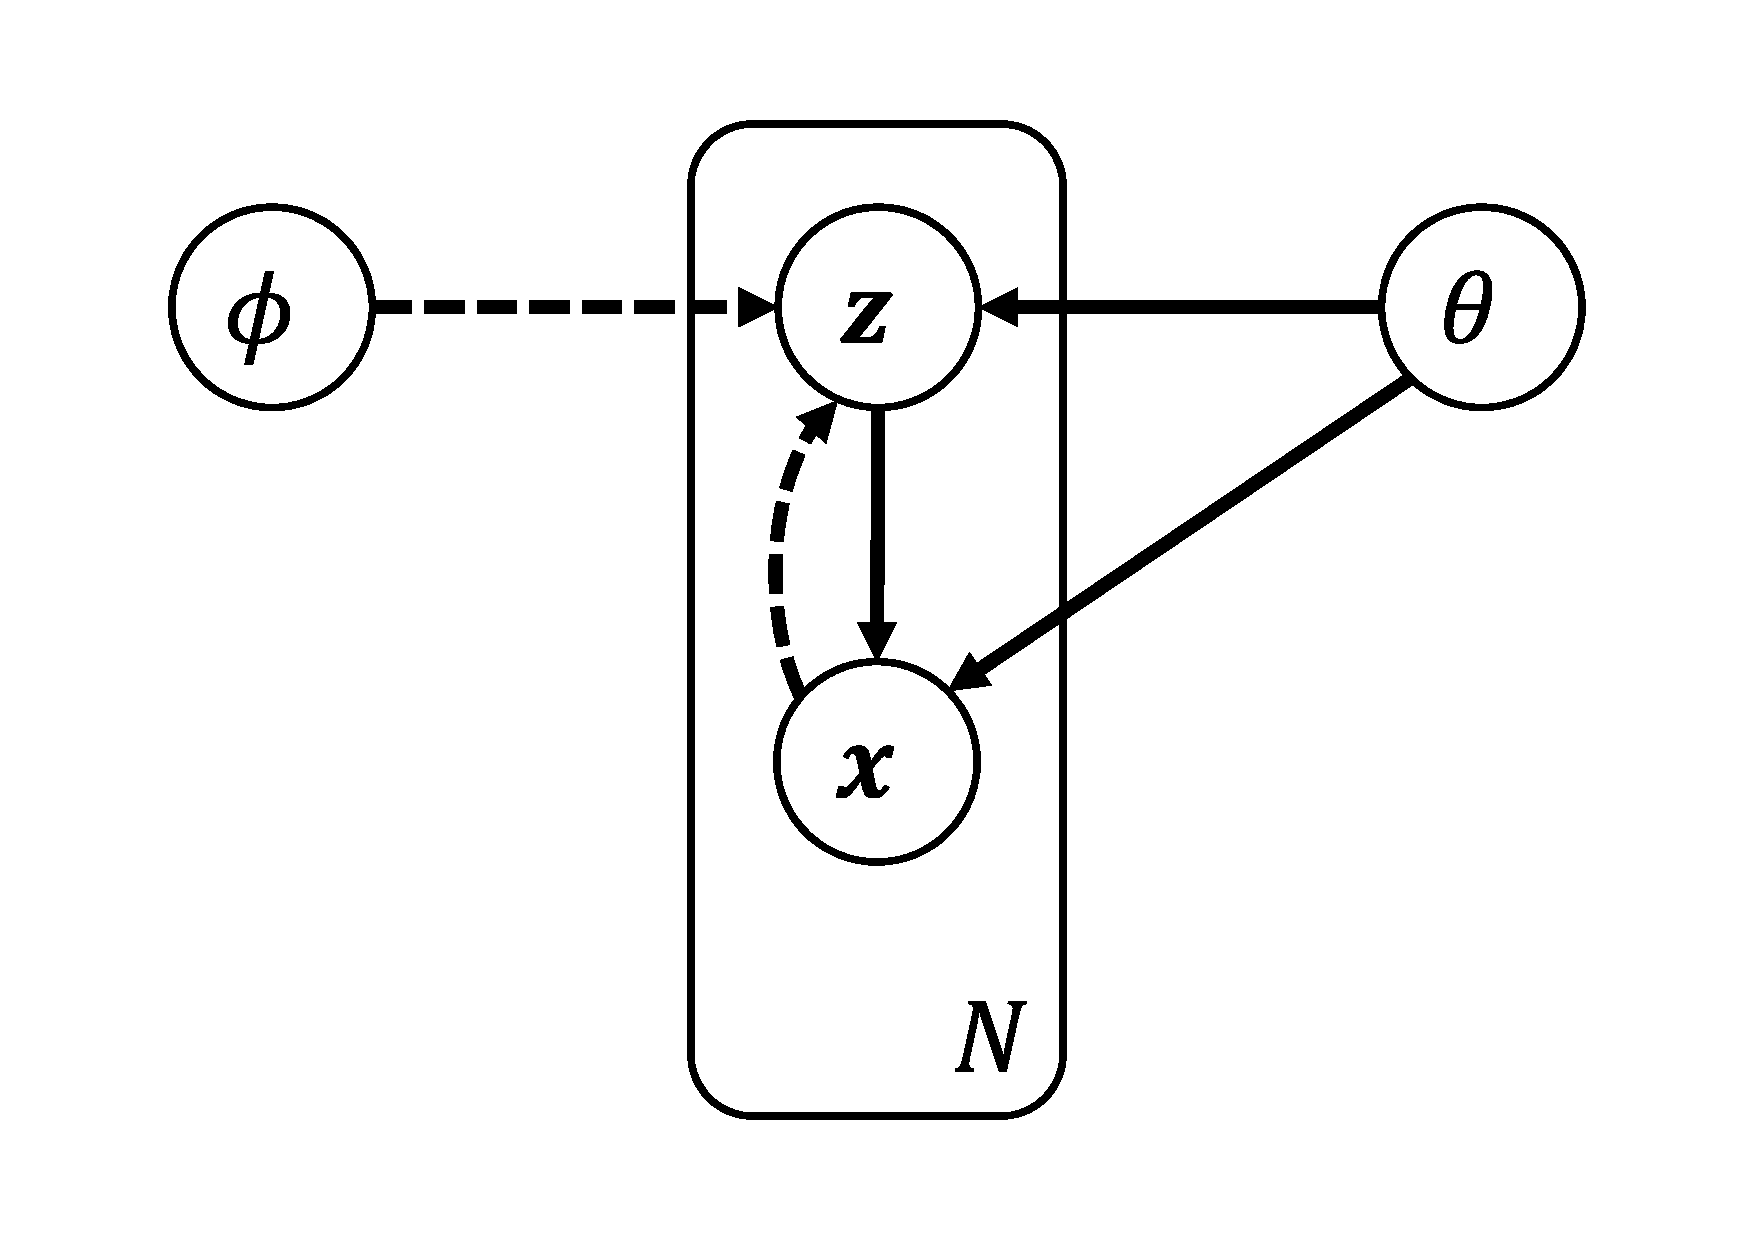
\includegraphics[keepaspectratio,scale=0.2]{vae-graphical-model.pdf}
	\caption{変分自己符号化器(VAE)におけるグラフィカルモデル}
	\label{fig:vae-graphical-model}
\end{figure}

\end{frame}

\begin{frame}{変分自己符号化器(VAE)の概要}

\begin{itemize}
	\item 確率分布のニューラルネットワークによる表現
	\begin{itemize}
		\item 潜在変数を含む確率モデルについて、パラメータの最尤解を求めるために、EMアルゴリズムを導出した
		\item EMアルゴリズムでは、潜在変数に関する事後分布$p(\bm{z} | \bm{x}, \theta)$を計算する必要があった
		\item この事後分布$p(\bm{z} | \bm{x}, \theta)$の計算が困難であるとき、$p(\bm{z} | \bm{x}, \theta)$を別の分布$q(\bm{z} | \bm{x}, \phi)$で近似し、変分推論によって$q(\bm{z} | \phi)$の最適解を求めた
		\newline
		\item VAEは変分推論の変種であり、近似事後分布$q(\bm{z} | \bm{x}, \phi)$と、$p(\bm{x} | \bm{z}, \theta)$の2つを\alert{ニューラルネットワーク}で表現する
		\newline
		\item データ$\bm{x}$を潜在変数$\bm{z}$に対応付けるニューラルネットワークを、\alert{Encoder}という
		\item 潜在変数$\bm{z}$からデータ$\bm{x}$を復元するニューラルネットワークを、\alert{Decoder}という
		\item 分布$q(\bm{z} | \bm{x}, \phi)$は\alert{Encoder}、分布$p(\bm{x} | \bm{z}, \theta)$は\alert{Encoder}に相当する
	\end{itemize}
\end{itemize}

\end{frame}

\subsection{変分自己符号化器(VAE)の理論}

\begin{frame}{変分自己符号化器(VAE)の理論}

\begin{itemize}
	\item 変分自己符号化器(VAE)の理論
	\begin{itemize}
		\item 変分下界$\mathcal{L}(q)$は次のようであった
		\begin{eqnarray}
			\mathcal{L}(q) &=& \int q(\bm{z} | \bm{x}) \ln \frac{p(\bm{x}, \bm{z})}{q(\bm{z} | \bm{x})} d\bm{z} \\
			&=& \int q(\bm{z} | \bm{x}) \ln \frac{p(\bm{x} | \bm{z}) p(\bm{z})}{q(\bm{z} | \bm{x})} d\bm{z} \\
			&=& \int q(\bm{z} | \bm{x}) \ln p(\bm{x} | \bm{z}) d\bm{z} + \int q(\bm{z} | \bm{x}) \ln \frac{p(\bm{z})}{q(\bm{z} | \bm{x})} d\bm{z} \\
			&=& \int q(\bm{z} | \bm{x}) \ln p(\bm{x} | \bm{z}) d\bm{z} - \KL(q(\bm{z} | \bm{x}) || p(\bm{z})) \\
			&=& \mathbb{E}_{\bm{z} \sim q(\bm{z} | \bm{x})} \left[ \ln p(\bm{x} | \bm{z}) \right] - \KL(q(\bm{z} | \bm{x}) || p(\bm{z}))
		\end{eqnarray}
		
		\item ここでは、単一のデータ$\bm{x}$と、それに対応する潜在変数$\bm{z}$を考えている
		\item また、パラメータ$\theta, \phi$は省略している
		\newline
		
		\item \alert{第1項}$\mathbb{E}_{\bm{z} \sim q(\bm{z} | \bm{x})} \left[ \ln p(\bm{x} | \bm{z}) \right]$を\alert{大きく}、また\alert{第2項}$\KL(q(\bm{z} | \bm{x}) || p(\bm{z}))$を\alert{小さく}することで、変分下界$\mathcal{L}(q)$を大きくできる
		\newline
		\item VAEでは、変分下界$\mathcal{L}(q)$を最大化するパラメータ$\theta, \phi$を求めるために、ニューラルネットを使用する (変分推論にニューラルネットをねじ込んだもの)
		\newline
		
		\item KLダイバージェンスの項は、後ほど求めることにする(解析的に求められる)
		\item 第1項は、分布$q(\bm{z} | \bm{x})$に関する期待値であり、VAEでは\alert{サンプリングで近似}する
		\begin{equation}
			\mathbb{E}_{\bm{z} \sim q(\bm{z} | \bm{x})} \left[ \ln p(\bm{x} | \bm{z}) \right] \simeq \frac{1}{L} \sum_{l = 1}^L \ln p(\bm{x}_i | \bm{z}_{i, l})
		\end{equation}
		
		\item これより、変分下界$\mathcal{L}(q)$は以下のように書ける
		\begin{equation}
			\mathcal{L}(q) \simeq -\KL(q(\bm{z} | \bm{x}) || p(\bm{z})) + \frac{1}{L} \sum_{i = 1}^L \ln p(\bm{x}_i | \bm{z}_{i, l})
		\end{equation}
		
		\item パラメータ$\theta, \phi$を含めれば、次のように書ける
		\begin{equation}
			\mathcal{L}(q) \simeq -\KL(q(\bm{z} | \bm{x}, \phi) || p(\bm{z} | \theta)) + \frac{1}{L} \sum_{i = 1}^L \ln p(\bm{x}_i | \bm{z}_{i, l}, \theta)
		\end{equation}
	\end{itemize}
\end{itemize}

\end{frame}

\begin{frame}{変分自己符号化器(VAE)の理論}
	
\begin{itemize}
	\item Encoderのニューラルネットの入出力
	\begin{itemize}
		\item Encoderは、分布$q(\bm{z} | \bm{x}, \phi)$を表現するニューラルネット
		\item 入力$\bm{x}$に対応する潜在変数$\bm{z}$を得る
		\newline
		\item Encoderの入力は、明らかにデータ$\bm{x}$である
		\newline
		
		\item 変分下界$\mathcal{L}(q)$において、項$\mathbb{E}_{\bm{z}} \left[ \ln p(\bm{x} | \bm{z}) \right]$は近似する必要があった
		\item $\bm{z}$を、分布$q(\bm{z} | \bm{x}, \phi)$から$L$回サンプリングした
		\newline
		
		\item ニューラルネットで、$\bm{x}$から$\bm{z}$を\alert{直接サンプリングするのは困難}
		\item そこで、Encoderでは、サンプルされたデータは出力しないことにする
		\item その代わりに、サンプルする\alert{分布のパラメータを出力}する
		\newline
		\item 例えば、サンプルする分布が\alert{ガウス分布}であれば、\alert{平均}と\alert{分散}の2つのパラメータを出力する
		\newline
		\item 後述のように、分布$q(\bm{z} | \bm{x}, \phi)$は\alert{ガウス分布}になるので、Encoderは\alert{平均ベクトル}$\bm{\mu}$と\alert{共分散行列}$\bm{\Sigma}$を出力する
		\item 共分散行列は、実際には\alert{対角行列}であるため、実際には行列ではなく、\alert{行列の対角成分を要素にもつベクトル}を出力する
	\end{itemize}
\end{itemize}

\end{frame}

\begin{frame}{変分自己符号化器(VAE)の理論}
	
\begin{itemize}	
	\item Encoderの損失関数
	\begin{itemize}
		\item VAEでは、\alert{事前分布として}、平均ベクトル$\bm{0}$、共分散行列$\bm{I}$の\color{red}ガウス分布$\mathcal{N}(\bm{z} | \bm{0}, \bm{I})$を仮定\normalcolor する
		\newline
		\item データ$\bm{x}$は高次元だが、実際にはそのうちの\alert{低次元な領域にまとまって存在}する(\alert{多様体仮説})
		\item 従って、データ$\bm{x}$の構造を、\alert{より低次元な潜在変数$\bm{z}$の空間}$\bm{z} \sim \mathcal{N}(\bm{z} | \bm{0}, \bm{I})$\alert{に押し込める}ことができる
		\newline
		
		\item Encoderの損失関数は、\alert{KLダイバージェンス}$\KL(q(\bm{z} | \bm{x}, \phi) || p(\bm{z} | \theta))$で定義できる
		\item このKLダイバージェンスを最小化することは、Encoderの分布$q(\bm{z} | \bm{x}, \phi)$を、$p(\bm{z} | \theta) \sim \mathcal{N}(\bm{z} | \bm{0}, \bm{I})$に近づける制約に相当する
		\newline
		
		\item $p(\bm{z} | \theta)$がガウス分布であれば、事後分布$p(\bm{z} | \bm{x}, \theta)$もガウス分布であり、従って\color{red}$q(\bm{z} | \bm{x}, \phi)$もガウス分布\normalcolor となる
		\newline
		\item よって$\KL(q(\bm{z} | \bm{x}, \phi) || p(\bm{z} | \theta))$は、2つのガウス分布間のKLダイバージェンスである
		\newline
		
		\item 一般に、2つのガウス分布$p(\bm{z}) = \mathcal{N}(\bm{z} | \bm{\mu}_0, \bm{\Sigma}_0)$、$q(\bm{z}) = \mathcal{N}(\bm{z} | \bm{\mu}_1, \bm{\Sigma}_1)$間のKLダイバージェンスは、解析的に計算できる
		
		\item KLダイバージェンス$\KL(p(\bm{z}) || q(\bm{z}))$を順番に求めてみよう
		\begin{eqnarray}
			&& \KL(p(\bm{z}) || q(\bm{z})) \nonumber \\
			&=& \int p(\bm{z}) \ln \frac{p(\bm{z})}{q(\bm{z})} d\bm{z} \\
			&=& \int p(\bm{z}) \left( \ln p(\bm{z}) - \ln q(\bm{z}) \right) d\bm{z} \\
			&=& \int p(\bm{z}) \left( \ln \mathcal{N}(\bm{z} | \bm{\mu}_0, \bm{\Sigma}_0) - \ln \mathcal{N}(\bm{z} | \bm{\mu}_1, \bm{\Sigma}_1) \right) d\bm{z} \\
			&=& \mathbb{E}_{\bm{z} \sim p(\bm{z})} \left[ \ln \mathcal{N}(\bm{z} | \bm{\mu}_0, \bm{\Sigma}_0) - \ln \mathcal{N}(\bm{z} | \bm{\mu}_1, \bm{\Sigma}_1) \right]
		\end{eqnarray}
		
		\item データを$D$次元、潜在変数を$K$次元とする
		
		\item ここで
		\begin{eqnarray}
			&& \ln \mathcal{N}(\bm{z} | \bm{\mu}_0, \bm{\Sigma}_0) \nonumber \\
			&=& \ln \left( \frac{1}{(2\pi)^\frac{K}{2}} \frac{1}{|\bm{\Sigma}_0|^\frac{1}{2}} \exp \left( -\frac{1}{2} \left( \bm{z} - \bm{\mu}_0 \right)^T \bm{\Sigma}_0^{-1} \left( \bm{z} - \bm{\mu}_0 \right) \right) \right) \nonumber \\
			&=& -\frac{K}{2} \ln 2\pi - \frac{1}{2} \ln |\bm{\Sigma}_0| - \frac{1}{2} \left( \bm{z} - \bm{\mu}_0 \right)^T \bm{\Sigma}_0^{-1} \left( \bm{z} - \bm{\mu}_0 \right)
		\end{eqnarray}
		\begin{eqnarray}
			&& \ln \mathcal{N}(\bm{z} | \bm{\mu}_1, \bm{\Sigma}_1) \nonumber \\
			&=& -\frac{K}{2} \ln 2\pi - \frac{1}{2} \ln |\bm{\Sigma}_1| - \frac{1}{2} \left( \bm{z} - \bm{\mu}_1 \right)^T \bm{\Sigma}_1^{-1} \left( \bm{z} - \bm{\mu}_1 \right)
		\end{eqnarray}
		であるので
		\begin{eqnarray}
			&& \ln \mathcal{N}(\bm{z} | \bm{\mu}_0, \bm{\Sigma}_0) - \ln \mathcal{N}(\bm{z} | \bm{\mu}_1, \bm{\Sigma}_1) \nonumber \\
			&=& -\frac{K}{2} \ln 2\pi - \frac{1}{2} \ln |\bm{\Sigma}_0| - \frac{1}{2} \left( \bm{z} - \bm{\mu}_0 \right)^T \bm{\Sigma}_0^{-1} \left( \bm{z} - \bm{\mu}_0 \right) - \nonumber \\
			&& \qquad \left( -\frac{K}{2} \ln 2\pi - \frac{1}{2} \ln |\bm{\Sigma}_1| - \frac{1}{2} \left( \bm{z} - \bm{\mu}_1 \right)^T \bm{\Sigma}_1^{-1} \left( \bm{z} - \bm{\mu}_1 \right) \right) \nonumber \\
			&=& \frac{1}{2} \ln \frac{|\bm{\Sigma}_1|}{|\bm{\Sigma}_0|} - \frac{1}{2} \left( \bm{z} - \bm{\mu}_0 \right)^T \bm{\Sigma}_0^{-1} \left( \bm{z} - \bm{\mu}_0 \right) + \nonumber \\
			&& \qquad \frac{1}{2} \left( \bm{z} - \bm{\mu}_1 \right)^T \bm{\Sigma}_1^{-1} \left( \bm{z} - \bm{\mu}_1 \right)
		\end{eqnarray}
		
		\item よって
		\begin{eqnarray}
			&& \KL(p(\bm{z}) || q(\bm{z})) \nonumber \\
			&=& \mathbb{E}_{\bm{z} \sim p(\bm{z})} \left[ \ln \mathcal{N}(\bm{z} | \bm{\mu}_0, \bm{\Sigma}_0) - \ln \mathcal{N}(\bm{z} | \bm{\mu}_1, \bm{\Sigma}_1) \right] \nonumber \\
			&=& \mathbb{E}_{p(\bm{z})} \left[ \frac{1}{2} \ln \frac{|\bm{\Sigma}_1|}{|\bm{\Sigma}_0|} - \frac{1}{2} \left( \bm{z} - \bm{\mu}_0 \right)^T \bm{\Sigma}_0^{-1} \left( \bm{z} - \bm{\mu}_0 \right) + \right. \nonumber \\
			&& \qquad \left. \frac{1}{2} \left( \bm{z} - \bm{\mu}_1 \right)^T \bm{\Sigma}_1^{-1} \left( \bm{z} - \bm{\mu}_1 \right) \right] \\
			&=& \frac{1}{2} \ln \frac{|\bm{\Sigma}_1|}{|\bm{\Sigma}_0|} - \frac{1}{2} \mathbb{E}_{p(\bm{z})} \left[ \left( \bm{z} - \bm{\mu}_0 \right)^T \bm{\Sigma}_0^{-1} \left( \bm{z} - \bm{\mu}_0 \right) \right] + \nonumber \\
			&& \qquad \frac{1}{2} \mathbb{E}_{p(\bm{z})} \left[ \left( \bm{z} - \bm{\mu}_1 \right)^T \bm{\Sigma}_1^{-1} \left( \bm{z} - \bm{\mu}_1 \right) \right]
		\end{eqnarray}
		
		\item ここで、期待値についての式を導出しておく
		\item $\mathbb{E} \left[ \bm{z} \right] = \bm{\mu}$、$\mathbb{E} \left[ \left( \bm{z} - \bm{\mu} \right) \left( \bm{z} - \bm{\mu} \right)^T \right] = \bm{\Sigma}$とする
		\item $\bm{z}$の$i$成分を$z_i$、$\bm{\mu}$の$i$成分を$\mu_i$、$\bm{\Sigma}$の$i, j$成分を$\Sigma_{ij}$とする
		\newline
		
		\item このとき
		\begin{eqnarray}
			\Sigma_{ij}
			&=& \mathbb{E} \left[ \left( z_i - \mu_i \right) \left( z_j - \mu_j \right) \right] \nonumber \\
			&=& \mathbb{E} \left[ z_i z_j - z_i \mu_j - z_j \mu_i + \mu_i \mu_j \right] \nonumber \\
			&=& \mathbb{E} \left[ z_i z_j \right] - \mu_j \mathbb{E} \left[ z_i \right] - \mu_i \mathbb{E} \left[ z_j \right] + \mu_i \mu_j \nonumber \\
			&=& \mathbb{E} \left[ z_i z_j \right] - \mu_j \mu_i - \mu_i \mu_j + \mu_i \mu_j \nonumber \\
			&=& \mathbb{E} \left[ z_i z_j \right] + \mu_i \mu_j
		\end{eqnarray}
		であるから
		\begin{equation}
			\mathbb{E} \left[ z_i z_j \right] = \Sigma_{ij} - \mu_i \mu_j
		\end{equation}
		
		\item そして、行列$\bm{A}$の$i, j$成分を$A_{ij}$とすれば、以下を得る
		\begin{eqnarray}
			\mathbb{E} \left[ \bm{z}^T \bm{A} \bm{z} \right]
			&=& \mathbb{E} \left[ \sum_i \sum_j z_i A_{ij} z_j \right] \nonumber \\
			&=& \sum_i \sum_j A_{ij} \mathbb{E} \left[ z_i z_j \right] \nonumber \\
			&=& \sum_i \sum_j A_{ij} \left( \Sigma_{ij} + \mu_i \mu_j \right) \nonumber \\
			&=& \sum_i \sum_j A_{ij} \Sigma_{ij} + \sum_i \sum_j A_{ij} \mu_i \mu_j \nonumber \\
			&=& \sum_i \sum_j A_{ij} \Sigma_{\color{red}ji\normalcolor} + \sum_i \sum_j \mu_i A_{ij} \mu_j \nonumber \\
			&=& \sum_i \left( \bm{A} \bm{\Sigma} \right)_{ii} + \bm{\mu}^T \bm{A} \bm{\mu} \nonumber \\
			&=& \Tr \left( \bm{A} \bm{\Sigma} \right) + \bm{\mu}^T \bm{A} \bm{\mu}
		\end{eqnarray}
		
		\item 上式の変形では、共分散行列$\bm{\Sigma}$が対称行列ゆえ、$\Sigma_{ij} = \Sigma_{ji}$が成立することを用いた
		
		\item また、ベクトル$\bm{a}$の$i$成分を$a_i$とすれば、以下を得る
		\begin{eqnarray}
			\mathbb{E} \left[ \bm{a}^T \bm{z} \right]
			&=& \mathbb{E} \left[ \bm{z}^T \bm{a} \right] \nonumber \\
			&=& \mathbb{E} \left[ \sum_i z_i a_i \right] \nonumber \\
			&=& \sum_i a_i \mathbb{E} \left[ z_i \right] \nonumber \\
			&=& \sum_i a_i \mu_i \nonumber \\
			&=& \bm{a}^T \bm{\mu} = \bm{\mu}^T \bm{a}
		\end{eqnarray}
		
		\item これより、$\bm{a}, \bm{B}$をそれぞれ適当なベクトル、行列とすれば、以下を得る
		\begin{eqnarray}
			&& \mathbb{E} \left[ \left( \bm{z} - \bm{a} \right)^T \bm{B} \left( \bm{z} - \bm{a} \right) \right] \nonumber \\
			&=& \mathbb{E} \left[ \bm{z}^T \bm{B} \bm{z} - \bm{z}^T \bm{B} \bm{a} - \bm{a}^T \bm{B} \bm{z} + \bm{a}^T \bm{B} \bm{a} \right] \nonumber \\
			&=& \mathbb{E} \left[ \bm{z}^T \bm{B} \bm{z} \right] - \mathbb{E} \left[ \bm{z}^T \bm{B} \bm{a} \right] - \mathbb{E} \left[ \bm{a}^T \bm{B} \bm{z} \right] + \bm{a}^T \bm{B} \bm{a} \nonumber \\
			&=& \left( \Tr \left( \bm{B} \bm{\Sigma} \right) + \bm{\mu}^T \bm{B} \bm{\mu} \right) - \bm{\mu}^T \bm{B} \bm{a} - \bm{a}^T \bm{B} \bm{\mu} + \bm{a}^T \bm{B} \bm{a} \nonumber \\
			&=& \Tr \left( \bm{B} \bm{\Sigma} \right) + \bm{\mu}^T \bm{B} \bm{\mu} - 2 \bm{\mu}^T \bm{B} \bm{a} + \bm{a}^T \bm{B} \bm{a}
		\end{eqnarray}
		特に、$\bm{a} = \bm{\mu}, \bm{B} = \bm{\Sigma}^{-1}$とすれば
		\begin{eqnarray}
			&& \mathbb{E} \left[ \left( \bm{z} - \bm{\mu} \right)^T \bm{\Sigma}^{-1} \left( \bm{z} - \bm{\mu} \right) \right] \nonumber \\
			&=& \Tr \left( \bm{\Sigma}^{-1} \bm{\Sigma} \right) + \bm{\mu}^T \bm{\Sigma}^{-1} \bm{\mu} - 2 \bm{\mu}^T \bm{\Sigma}^{-1} \bm{\mu} + \bm{\mu}^T \bm{\Sigma}^{-1} \bm{\mu} \nonumber \\
			&=& \Tr \left( \bm{\Sigma}^{-1} \bm{\Sigma} \right) \nonumber \\
			&=& \Tr \left( \bm{I} \right) = K
		\end{eqnarray}
		
		\item これを用いれば、KLダイバージェンスは次のようになる
		\begin{eqnarray}
			&& \KL(p(\bm{z}) || q(\bm{z})) \nonumber \\
			&=& \frac{1}{2} \ln \frac{|\bm{\Sigma}_1|}{|\bm{\Sigma}_0|} - \frac{1}{2} \mathbb{E}_{p(\bm{z})} \left[ \left( \bm{z} - \bm{\mu}_0 \right)^T \bm{\Sigma}_0^{-1} \left( \bm{z} - \bm{\mu}_0 \right) \right] + \nonumber \\
			&& \qquad \frac{1}{2} \mathbb{E}_{p(\bm{z})} \left[ \left( \bm{z} - \bm{\mu}_1 \right)^T \bm{\Sigma}_1^{-1} \left( \bm{z} - \bm{\mu}_1 \right) \right] \nonumber \\
			&=& \frac{1}{2} \ln \frac{|\bm{\Sigma}_1|}{|\bm{\Sigma}_0|} - \frac{1}{2} K + \frac{1}{2} \left( \Tr \left( \bm{\Sigma}_1^{-1} \bm{\Sigma}_0 \right) + \bm{\mu}_0^T \bm{\Sigma}_1^{-1} \bm{\mu}_0 - \right. \nonumber \\
			&& \qquad \left. 2 \bm{\mu}_0^T \bm{\Sigma}_1^{-1} \bm{\mu}_1 + \bm{\mu}_1^T \bm{\Sigma}_1^{-1} \bm{\mu}_1 \right) \nonumber \\
			&=& \frac{1}{2} \ln \frac{|\bm{\Sigma}_1|}{|\bm{\Sigma}_0|} - \frac{1}{2} K + \frac{1}{2} \Tr \left( \bm{\Sigma}_1^{-1} \bm{\Sigma}_0 \right) + \nonumber \\
			&& \qquad \frac{1}{2} \left( \bm{\mu}_0 - \bm{\mu}_1 \right)^T \bm{\Sigma}_1^{-1} \left( \bm{\mu}_0 - \bm{\mu}_1 \right) \nonumber \\
			&=& \frac{1}{2} \left( \ln \frac{|\bm{\Sigma}_1|}{|\bm{\Sigma}_0|} - K + \Tr \left( \bm{\Sigma}_1^{-1} \bm{\Sigma}_0 \right) + \right. \nonumber \\
			&& \qquad \left( \bm{\mu}_0 - \bm{\mu}_1 \right)^T \bm{\Sigma}_1^{-1} \left( \bm{\mu}_0 - \bm{\mu}_1 \right) \bigg)
		\end{eqnarray}
		
		\item これで、2つのガウス分布$p(\bm{z}) = \mathcal{N}(\bm{z} | \bm{\mu}_0, \bm{\Sigma}_0)$、$q(\bm{z}) = \mathcal{N}(\bm{z} | \bm{\mu}_1, \bm{\Sigma}_1)$間のKLダイバージェンスが、次のようになることが分かった
		\begin{eqnarray}
			&& \KL(p(\bm{z}) || q(\bm{z})) \nonumber \\
			&=& \frac{1}{2} \left( \ln \frac{|\bm{\Sigma}_1|}{|\bm{\Sigma}_0|} - K + \Tr \left( \bm{\Sigma}_1^{-1} \bm{\Sigma}_0 \right) + \right. \nonumber \\
			&& \qquad \left( \bm{\mu}_0 - \bm{\mu}_1 \right)^T \bm{\Sigma}_1^{-1} \left( \bm{\mu}_0 - \bm{\mu}_1 \right) \bigg)
		\end{eqnarray}
		
		\item ここでは、$p(\bm{z}) = \mathcal{N}(\bm{z} | \bm{\mu}_0, \bm{\Sigma}_0)$は、Encoderのニューラルネットが表現する分布$q(\bm{z} | \bm{x}, \phi)$である
		\item そして、分布$q(\bm{z} | \bm{x}, \phi)$はガウス分布であったので、ここでは平均$\bm{\mu}_0$と共分散行列$\bm{\Sigma}_0$を使って、$q(\bm{z} | \bm{x}, \phi) = \mathcal{N}(\bm{z} | \bm{\mu}_0, \bm{\Sigma}_0)$と表すことにする
		\newline
		
		\item また$q(\bm{z}) = \mathcal{N}(\bm{z} | \bm{\mu}_1, \bm{\Sigma}_1)$は、潜在変数に関する事後分布$p(\bm{z} | \theta) = \mathcal{N}(\bm{z} | \bm{0}, \bm{I})$である
		\newline
		
		\item 結局、KLダイバージェンス$\KL(q(\bm{z} | \bm{x}, \phi) || p(\bm{z} | \theta))$は、先程の式に$\bm{\mu}_1 = \bm{0}$と$\bm{\Sigma}_1 = \bm{I}$を代入すれば得られる
		\begin{eqnarray}
			&& \KL(q(\bm{z} | \bm{x}, \phi) || p(\bm{z} | \theta)) \nonumber \\
			&=& \KL(\mathcal{N}(\bm{z} | \bm{\mu}_0, \bm{\Sigma}_0) || \mathcal{N}(\bm{z} | \bm{0}, \bm{I})) \nonumber \\
			&=& \color{red}\frac{1}{2} \left( -\ln |\bm{\Sigma}_0| - K + \Tr \left( \bm{\Sigma}_0 \right) + \bm{\mu}_0^T \bm{\mu}_0 \right)\normalcolor
		\end{eqnarray}
		
		\item このKLダイバージェンスが、Encoderの損失関数として定義される
		\newline
		\item Encoderのニューラルネットは、入力としてデータ$\bm{x}$を取り、平均$\bm{\mu}_0$と共分散行列$\bm{\Sigma}_0$を出力する
		\item 従って、Encoderの出力と、潜在変数の次元$K$を上式に代入すれば、損失関数を容易に計算できる
		\newline
		\item $\bm{\Sigma}_0$は\alert{対称行列}であるため、実際に出力されるのは、\color{red}$\bm{\Sigma}_0$の対角成分を並べたベクトル\normalcolor である
		\newline
		\item 一般的なVAEのEncoderは次の図\ref{fig:vae-encoder-architecture}のように表せる
	\end{itemize}
\end{itemize}

\end{frame}

\begin{frame}{変分自己符号化器(VAE)の理論}
	
\begin{figure}[h]
	\centering
	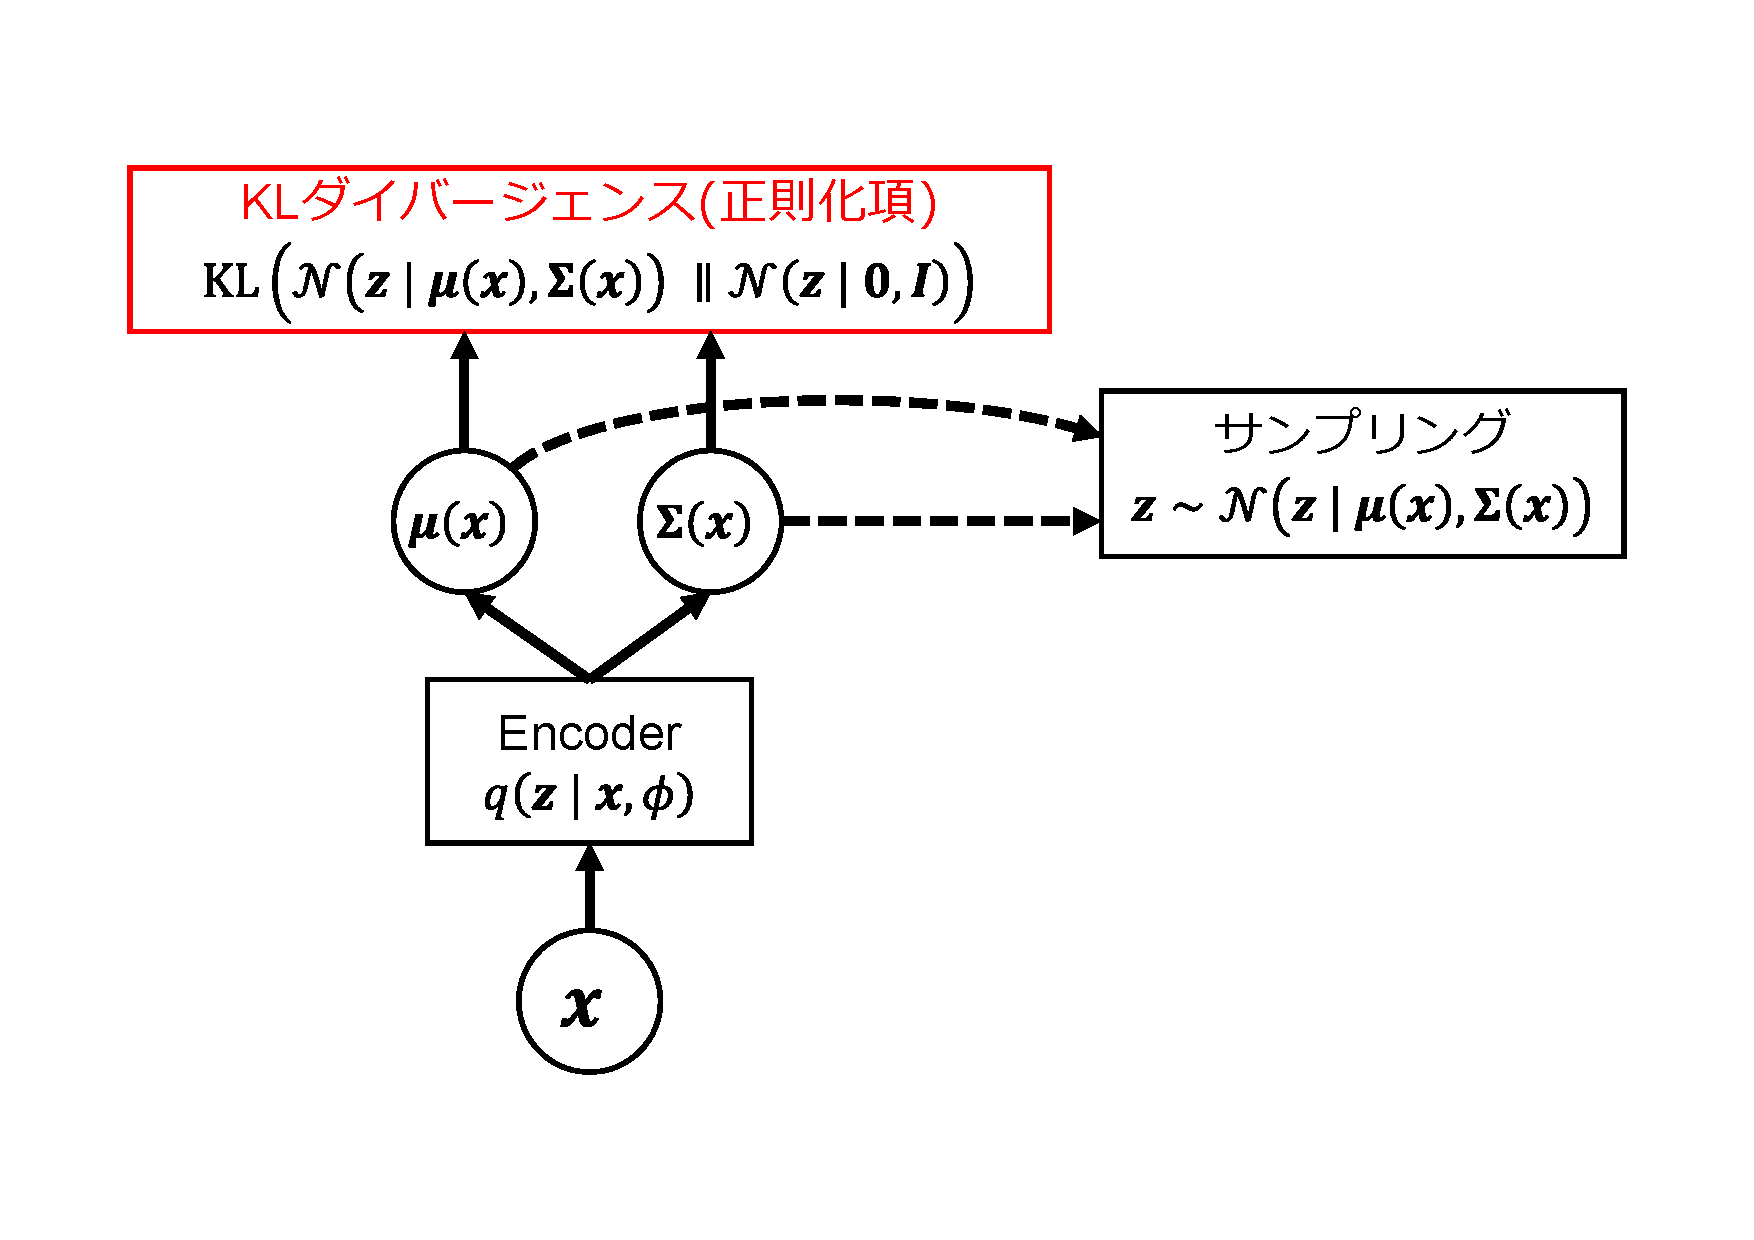
\includegraphics[keepaspectratio,scale=0.3,clip,trim=1cm 1cm 1cm 1cm]{vae-encoder-architecture.pdf}
	\caption{VAEのEncoderの概要}
	\label{fig:vae-encoder-architecture}
\end{figure}

\end{frame}

\begin{frame}{変分自己符号化器(VAE)の理論}
	
\begin{itemize}
	\item Encoderのニューラルネットの構造
	\begin{itemize}
		\item VAEが最初に提案された論文では、隠れ層は1層となっている
		\item 最終層は、$\bm{\mu}_0$と$\sqrt{\bm{\Sigma}_0}$を出力する2つのユニットから成る
		\item $\sqrt{\bm{\Sigma}_0}$とは、行列$\bm{\Sigma}_0$の各要素の平方根を取った行列である
		\newline
		
		\item 隠れ層の重みを$\bm{W}_h$、バイアスを$\bm{b}_h$、活性化関数を$f(\cdot)$、層の出力を$\bm{h}$とする
		\item 隠れ層で行う処理は、次の式で表される
		\begin{equation}
			\bm{h} = f(\bm{W}_h \bm{x} + \bm{b}_h)
		\end{equation}
		
		\item $\bm{\mu}_0$は、重み$\bm{W}_m$とバイアス$\bm{b}_m$を使って、以下のように計算される
		\begin{equation}
			\bm{\mu}_0 = \bm{W}_m \bm{h} + \bm{b}_m
		\end{equation}
		
		\item $\sqrt{\bm{\Sigma}_0}$は、重み$\bm{W}_s$とバイアス$\bm{b}_s$から、以下のように計算される
		\begin{equation}
			\sqrt{\bm{\Sigma}_0} = \bm{W}_s \bm{h} + \bm{b}_s
		\end{equation}
	\end{itemize}
\end{itemize}

\end{frame}

\begin{frame}{変分自己符号化器(VAE)の理論}

\begin{itemize}
	\item Decoderのニューラルネットの入出力
	\begin{itemize}
		\item Decoderは、分布$p(\bm{x} | \bm{z}, \theta)$を表現するニューラルネット
		\item 潜在変数$\bm{z}$から元のデータ$\bm{x}$を復元する
		\newline
	
		\item Decoderの入力は、Encoderによってサンプリングされた$\bm{z}$となる
		\newline
		\item もう少し正確に表現すると、Encoderから出力されるのは、分布のパラメータ$\bm{\mu}, \bm{\Sigma}$である
		\item そして、そのパラメータを使って分布$\mathcal{N}(\bm{z} | \bm{\mu}, \bm{\Sigma})$を構成し、分布から$\bm{z}$をサンプリングする
		\newline
		
		\item Decoderの出力は、復元されたデータ$\bm{y}$である
	\end{itemize}
\end{itemize}

\end{frame}

\begin{frame}{変分自己符号化器(VAE)の理論}

\begin{itemize}
	\item Decoderの損失関数
	\begin{itemize}
		\item 画像データでは通常、各ピクセルの値が$0$から$1$までになるように\alert{スケーリング}されている
		\item このとき、$p(\bm{x} | \bm{z})$は\alert{ベルヌーイ分布}と仮定していることになる
		\newline
		
		\item 出力層のユニット$j$は、$y_j = p(x_j = 1 | \bm{z})$を出力しているとみなせる
		\item $y_j$は、再構成$\bm{y}$の$j$番目の要素であり、元のデータ$\bm{x}$の$j$番目の要素$x_j$と対応する
		\newline
		\item VAEが最初に提案された論文では、隠れ層は1層のみである
		\item 再構成$\bm{y}$は、次のように計算される
		\begin{equation}
			\bm{y} = f_\sigma \left( \bm{W}_o \mathrm{tanh} \left( \bm{W}_h \bm{z} + \bm{b}_h \right) + \bm{b}_o \right)
		\end{equation}
		\item $f_\sigma(\cdot)$は、行列の各要素にシグモイド関数$\sigma(\cdot)$を適用する活性化関数
		\item $\bm{W}_h, \bm{b}_h$は隠れ層の重みとバイアス、$\bm{W}_o, \bm{b}_o$は出力層の重みとバイアス
		\newline
		
		\item このとき$\ln p(\bm{x} | \bm{z})$は次のように記述できる
		\begin{eqnarray}
			\ln p(\bm{x} | \bm{z}) &=& \ln \prod_{j = 1}^D \left( p(x_j = 1 | \bm{z}) \right)^{x_j} \left( p(x_j = 0 | \bm{z}) \right)^{1 - x_j} \nonumber \\
			&=& \ln \prod_j \left( p(x_j = 1 | \bm{z}) \right)^{x_j} \left( 1 - p(x_j = 1 | \bm{z}) \right)^{1 - x_j} \nonumber \\
			&=& \ln \prod_j y_j^{x_j} \left( 1 - y_j \right)^{1 - x_j} \nonumber \\
			&=& \sum_j \left( x_j \ln y_j + \left( 1 - x_j \right) \ln \left( 1 - y_j \right) \right)
		\end{eqnarray}
		
		\item $\bm{z}$は、分布$q(\bm{z} | \bm{x}, \phi)$からサンプリングされている
		\item 従って、上記を最大化することは、$\mathbb{E}_{q(\bm{z})} \left[ \ln p(\bm{x} | \bm{z}) \right]$を最大化することに等しい
		\newline
		
		\item 上記は、$x_j$と$y_j$のいずれもベルヌーイ分布に従う(二値変数)ときの、\alert{負の交差エントロピー}となっていることが分かる
		\item 従って、$\mathbb{E}_{q(\bm{z})} \left[ \ln p(\bm{x} | \bm{z}) \right]$を最大化することは、\alert{交差エントロピーを最小化}することに相当
		\newline
		\item Decoderの損失関数は、以下の\alert{交差エントロピー誤差}として定義できる
		\begin{equation}
			E = - \sum_j \left( x_j \ln y_j + \left( 1 - x_j \right) \ln \left( 1 - y_j \right) \right)
		\end{equation}
		
		\item 元データ$x_j$と、その再構成$y_j$との\alert{差が大きければ大きいほど、上記の誤差は増大}する
		\item これより、上記の誤差は\alert{再構成誤差}(Reconstruction Error)とよばれる
		\newline
		
		\item これより、VAEのEncoderとDecoderは次の図\ref{fig:vae-architecture}のように表せる
	\end{itemize}
\end{itemize}

\end{frame}

\begin{frame}{変分自己符号化器(VAE)の理論}
	
\begin{figure}[h]
	\centering
	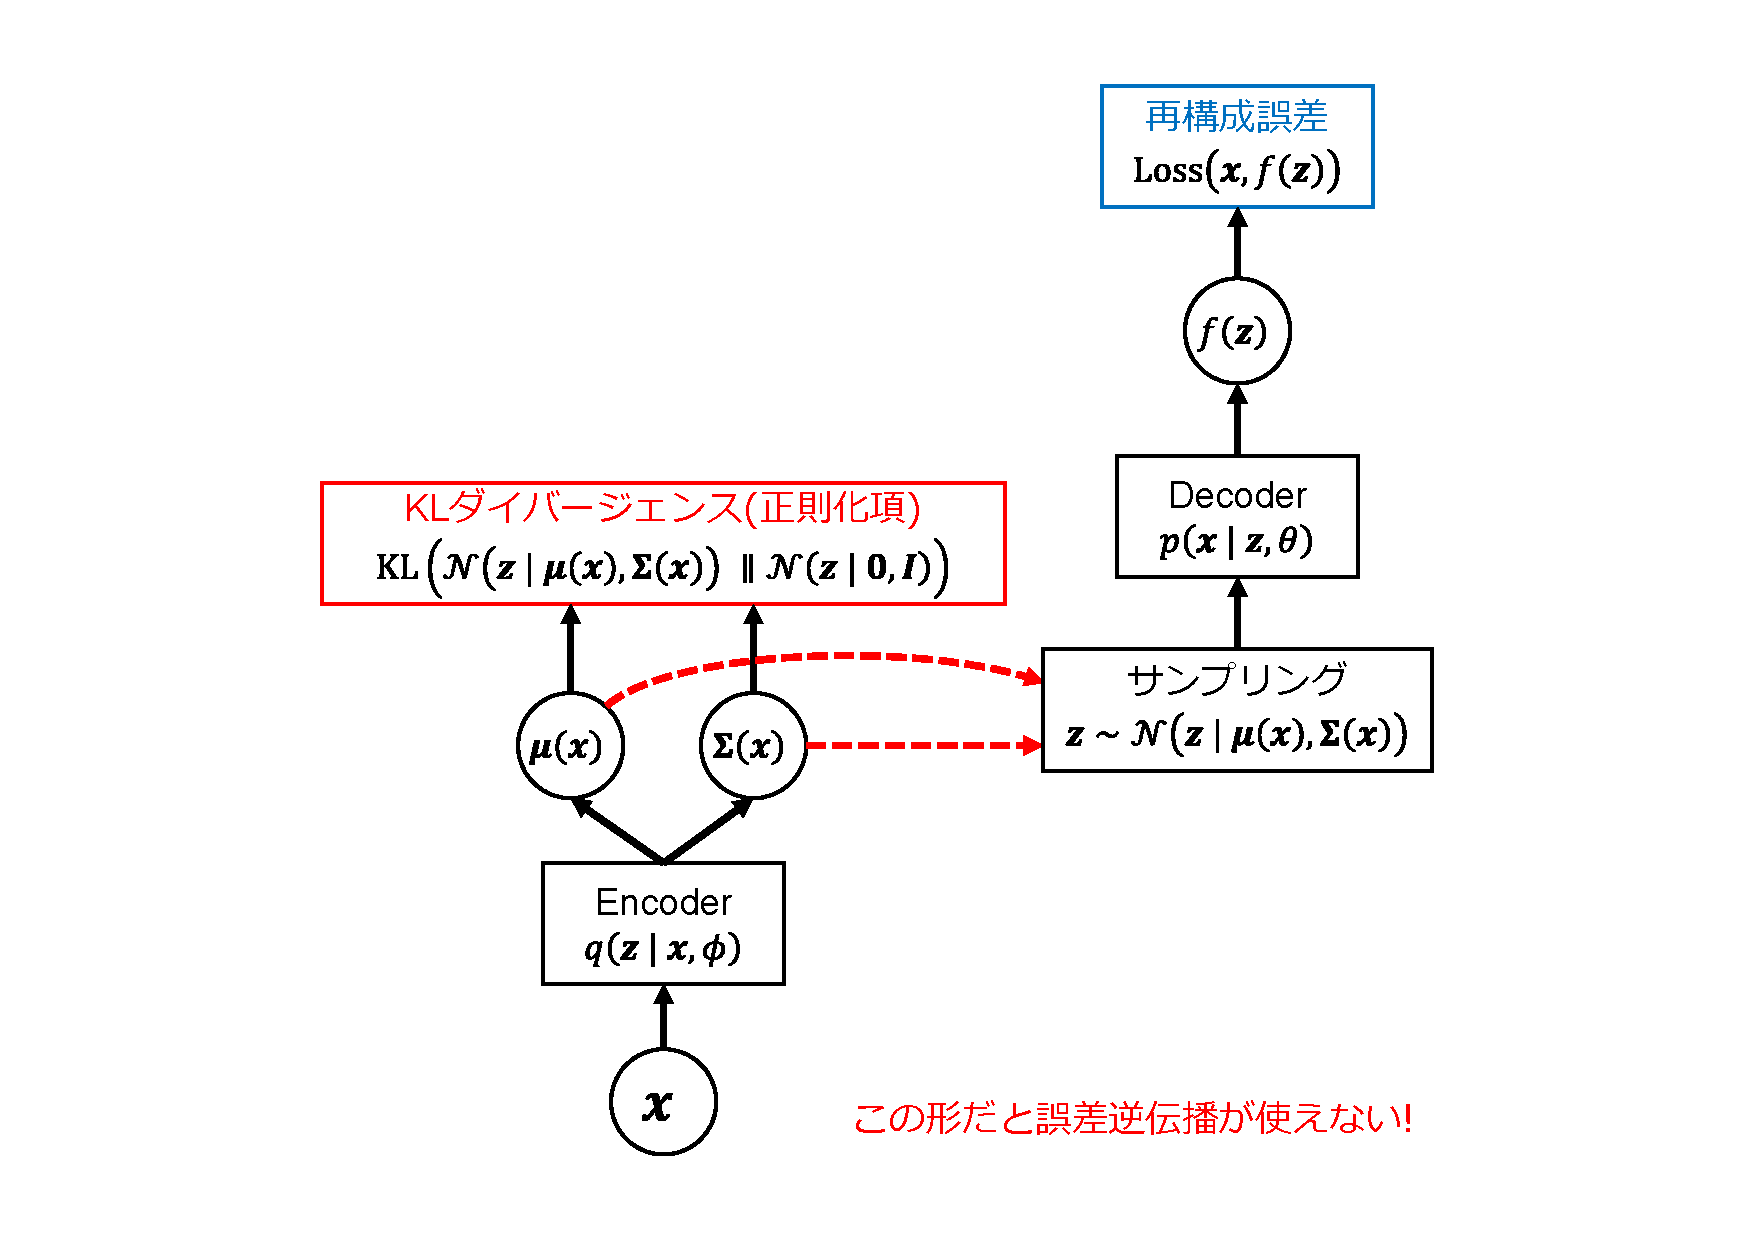
\includegraphics[keepaspectratio,scale=0.3,clip,trim=3cm 1cm 3cm 1cm]{vae-architecture.pdf}
	\caption{VAEのEncoderとDecoderの概要}
	\label{fig:vae-architecture}
\end{figure}

\end{frame}

\begin{frame}{変分自己符号化器(VAE)の理論}

\begin{itemize}
	\item Reparameterization Trick
	\begin{itemize}
		\item VAEが先程の図\ref{fig:vae-architecture}のようであるとき、\alert{大きな問題が生じる}
		\item サンプリングを行うと、計算グラフが途中で途切れるため、\alert{誤差逆伝播法を実行できない}
		\newline
		
		\item そこで、次の図\ref{fig:vae-actual-architecture}のように構成する
		\item $\bm{z} \sim \mathcal(\bm{z} | \bm{\mu}, \bm{\Sigma})$として、$\bm{z}$を分布から直接サンプリングするのではない
		\item $\bm{z}$を、\alert{決定論的な関数}$g(\bm{\epsilon}, \bm{x} | \phi)$から決定する
		\item 但し、$\bm{\epsilon}$は、分布$p(\bm{\epsilon})$からサンプリングされる
		\newline
		
		\item ニューラルネットの最適化には無関係な項$\bm{\epsilon}$と、Encoderのパラメータ$\phi$で$\bm{z}$を表現することで、誤差逆伝播法を実行可能にする
		\item このテクニックを、\alert{Reparameterization Trick}という
		\newline
		
		\item $\bm{\epsilon} \sim \mathcal(\bm{\epsilon} | \bm{0}, \bm{I})$とすれば、$\bm{z}$は次のように計算できる
		\begin{equation}
			\bm{z} = g(\bm{\epsilon}, \bm{x} | \phi) = \bm{\mu} + \bm{\Sigma}^\frac{1}{2} \bm{\epsilon}
		\end{equation}
		
		\item 共分散行列$\bm{\Sigma}$が対角行列であれば、上記の$\bm{\Sigma}^\frac{1}{2} \bm{\epsilon}$は、単なる要素ごとの積(対角行列の各要素を並べたベクトルと、$\bm{\epsilon}$の要素ごとの積)として書ける
		\newline
		
		\item $\bm{z}$の式は以下のように導出できる
		\newline
		
		\item 確率変数$\bm{z}, \bm{\epsilon}$間の関係が、次のようになっているとする
		\begin{equation}
			\bm{z} = \bm{\mu} + \bm{U} \bm{\Lambda}^\frac{1}{2} \bm{\epsilon}
		\end{equation}
		
		\item 但し、正定値対称行列$\bm{\Sigma}$が、固有値分解によって$\bm{\Sigma} = \bm{U} \bm{\Lambda} \bm{U}^T = \bm{U} \bm{\Lambda}^\frac{1}{2} \left( \bm{U} \bm{\Lambda} \right)^T$と表せるとする
		\item $\bm{U}$は固有ベクトルを並べた行列、$\bm{\Lambda}$は対角成分に固有値をもつ対角行列とする
		\newline
		
		\item 確率分布$p(\bm{z})$と$p(\bm{\epsilon})$との関係は、ヤコビ行列$\bm{J} = \partial \bm{\epsilon} / \partial \bm{z}$により次のように記述できる
		\begin{equation}
			p(\bm{z}) = p(\bm{\epsilon}) | \det \left( \bm{J} \right) | = p(\bm{\epsilon}) \left| \det \left( \frac{\partial \bm{z}}{\partial \bm{\epsilon}} \right) \right|
		\end{equation}
		
		\item ヤコビ行列$\bm{J}$を計算すると次のようになる
		\begin{equation}
			\bm{J} = \frac{\partial \bm{\epsilon}}{\partial \bm{y}} = \frac{\partial}{\partial \bm{z}} \left( \left( \bm{U} \bm{\Lambda}^\frac{1}{2} \right)^{-1} \left( \bm{z} - \bm{\mu} \right) \right) = \left( \left( \bm{U} \bm{\Lambda}^\frac{1}{2} \right)^{-1} \right)^T
		\end{equation}
		
		\item ヤコビ行列$\bm{J}$の行列式は次のようになる
		\begin{eqnarray}
			\det \left( \bm{J} \right) &=& \left| \left( \left( \bm{U} \bm{\Lambda}^\frac{1}{2} \right)^{-1} \right)^T \right| \nonumber \\
			&=& \left| \left( \bm{U} \bm{\Lambda}^\frac{1}{2} \right)^{-1} \right| \qquad (\because |\bm{A}^T| = |\bm{A}|) \nonumber \\
			&=& \frac{1}{\left| \bm{U} \bm{\Lambda}^\frac{1}{2} \right|} \qquad \left( \because |\bm{A}^{-1}| = \frac{1}{|\bm{A}|} \right) \nonumber \\
		\end{eqnarray}
		
		\item $\bm{\Sigma}$の行列式は次のように表せる
		\begin{equation}
			| \bm{\Sigma} | = \left| \bm{U} \bm{\Lambda}^\frac{1}{2} \left( \bm{U} \bm{\Lambda}^\frac{1}{2} \right)^T \right| = \left| \bm{U} \bm{\Lambda}^\frac{1}{2} \right| \left| \left( \bm{U} \bm{\Lambda}^\frac{1}{2} \right)^T \right| = \left| \bm{U} \bm{\Lambda}^\frac{1}{2} \right|^2
		\end{equation}
		
		\item 従って$\left| \bm{U} \bm{\Lambda}^\frac{1}{2} \right| = \left| \bm{\Sigma} \right|^\frac{1}{2}$である
		\item $\bm{\Sigma}$は正定値である($\left| \bm{\Sigma} \right| > 0$)から、$\left| \bm{\Sigma} \right|^\frac{1}{2} = \left| \bm{U} \bm{\Lambda}^\frac{1}{2} \right| > 0$が成立し、$\bm{U} \bm{\Lambda}^\frac{1}{2}$も正定値行列となる
		\item これより、逆行列$\left( \bm{U} \bm{\Lambda}^\frac{1}{2} \right)^{-1}$が存在するので、ヤコビ行列$\bm{J}$は計算できることが確認される
		\newline
		\item ヤコビ行列$\bm{J}$の行列式の絶対値は、次のようになる
		\begin{equation}
			\left| \det(\bm{J}) \right| = \left| \frac{1}{\left| \bm{U} \bm{\Lambda}^\frac{1}{2} \right|} \right| = \left| \frac{1}{\left| \bm{\Sigma} \right|^\frac{1}{2}} \right| = \frac{1}{\left| \bm{\Sigma} \right|^\frac{1}{2}}
		\end{equation}
		
		\item $p(\bm{\epsilon})$がガウス分布$\mathcal{N}(\bm{\epsilon} | \bm{0}, \bm{I})$であるとすると、$p(\bm{z})$は次のようになる
		\begin{eqnarray}
			p(\bm{z}) &=& p(\bm{\epsilon}) \left| \det \left( \frac{\partial \bm{z}}{\partial \bm{\epsilon}} \right) \right| \nonumber \\
			&=& \frac{1}{(2\pi)^\frac{K}{2}} \exp \left( -\frac{1}{2} \bm{\epsilon}^T \bm{\epsilon} \right) \frac{1}{|\bm{\Sigma}|^\frac{1}{2}}
		\end{eqnarray}
		
		\item ここで、指数関数の中身は次のように書ける
		\begin{eqnarray}
			&& \left( \bm{z} - \bm{\mu} \right)^T \bm{\Sigma}^{-1} \left( \bm{z} - \bm{\mu} \right) \nonumber \\
			&=& \left( \bm{U} \bm{\Lambda}^\frac{1}{2} \bm{\epsilon} \right)^T \left( \bm{U} \bm{\Lambda} \bm{U}^T \right)^{-1} \left( \bm{U} \bm{\Lambda}^\frac{1}{2} \bm{\epsilon} \right) \nonumber \\
			&=& \bm{\epsilon}^T \left( \bm{\Lambda}^\frac{1}{2} \right)^T \bm{U}^T \left( \bm{U}^T \right)^{-1} \bm{\Lambda}^{-1} \bm{U}^{-1} \bm{U} \bm{\Lambda}^\frac{1}{2} \bm{\epsilon} \nonumber \\
			&=& \bm{\epsilon}^T \left( \bm{\Lambda}^\frac{1}{2} \right)^T \bm{\Lambda}^{-1} \bm{\Lambda}^\frac{1}{2} \bm{\epsilon} \nonumber \\
			&=& \bm{\epsilon}^T \bm{\Lambda}^\frac{1}{2} \bm{\Lambda}^{-1} \bm{\Lambda}^\frac{1}{2} \bm{\epsilon} \nonumber \\
			&=& \bm{\epsilon}^T \bm{\epsilon}
		\end{eqnarray}
		
		\item これより、$p(\bm{z})$は平均$\bm{\mu}$、共分散行列$\bm{\Sigma}$のガウス分布である
		\begin{eqnarray}
			p(\bm{z}) &=& \frac{1}{(2\pi)^\frac{K}{2}} \exp \left( -\frac{1}{2} \bm{\epsilon}^T \bm{\epsilon} \right) \frac{1}{|\bm{\Sigma}|^\frac{1}{2}} \nonumber \\
			&=& \frac{1}{(2\pi)^\frac{K}{2}} \frac{1}{|\bm{\Sigma}|^\frac{1}{2}} \exp \left( -\frac{1}{2} \left( \bm{z} - \bm{\mu} \right)^T \bm{\Sigma}^{-1} \left( \bm{z} - \bm{\mu} \right) \right) \\
			&=& \mathcal{N}(\bm{z} | \bm{\mu}, \bm{\Sigma})
		\end{eqnarray}
		
		\item $\bm{z} \sim \mathcal{N}(\bm{z} | \bm{\mu}, \bm{\Sigma})$について、共分散行列$\bm{\Sigma}$が既に対角行列であれば、$\bm{U} = \bm{I}$、$\bm{\Lambda} = \bm{\Sigma}$であるので、結局以下が言える
		\begin{equation}
			\bm{z} = \bm{\mu} + \bm{U} \bm{\Lambda}^\frac{1}{2} \bm{\epsilon} = \bm{\mu} + \bm{\Sigma}^\frac{1}{2} \bm{\epsilon}
		\end{equation}
	\end{itemize}
\end{itemize}

\end{frame}

\begin{frame}{変分自己符号化器(VAE)の理論}
	
\begin{figure}[h]
	\centering
	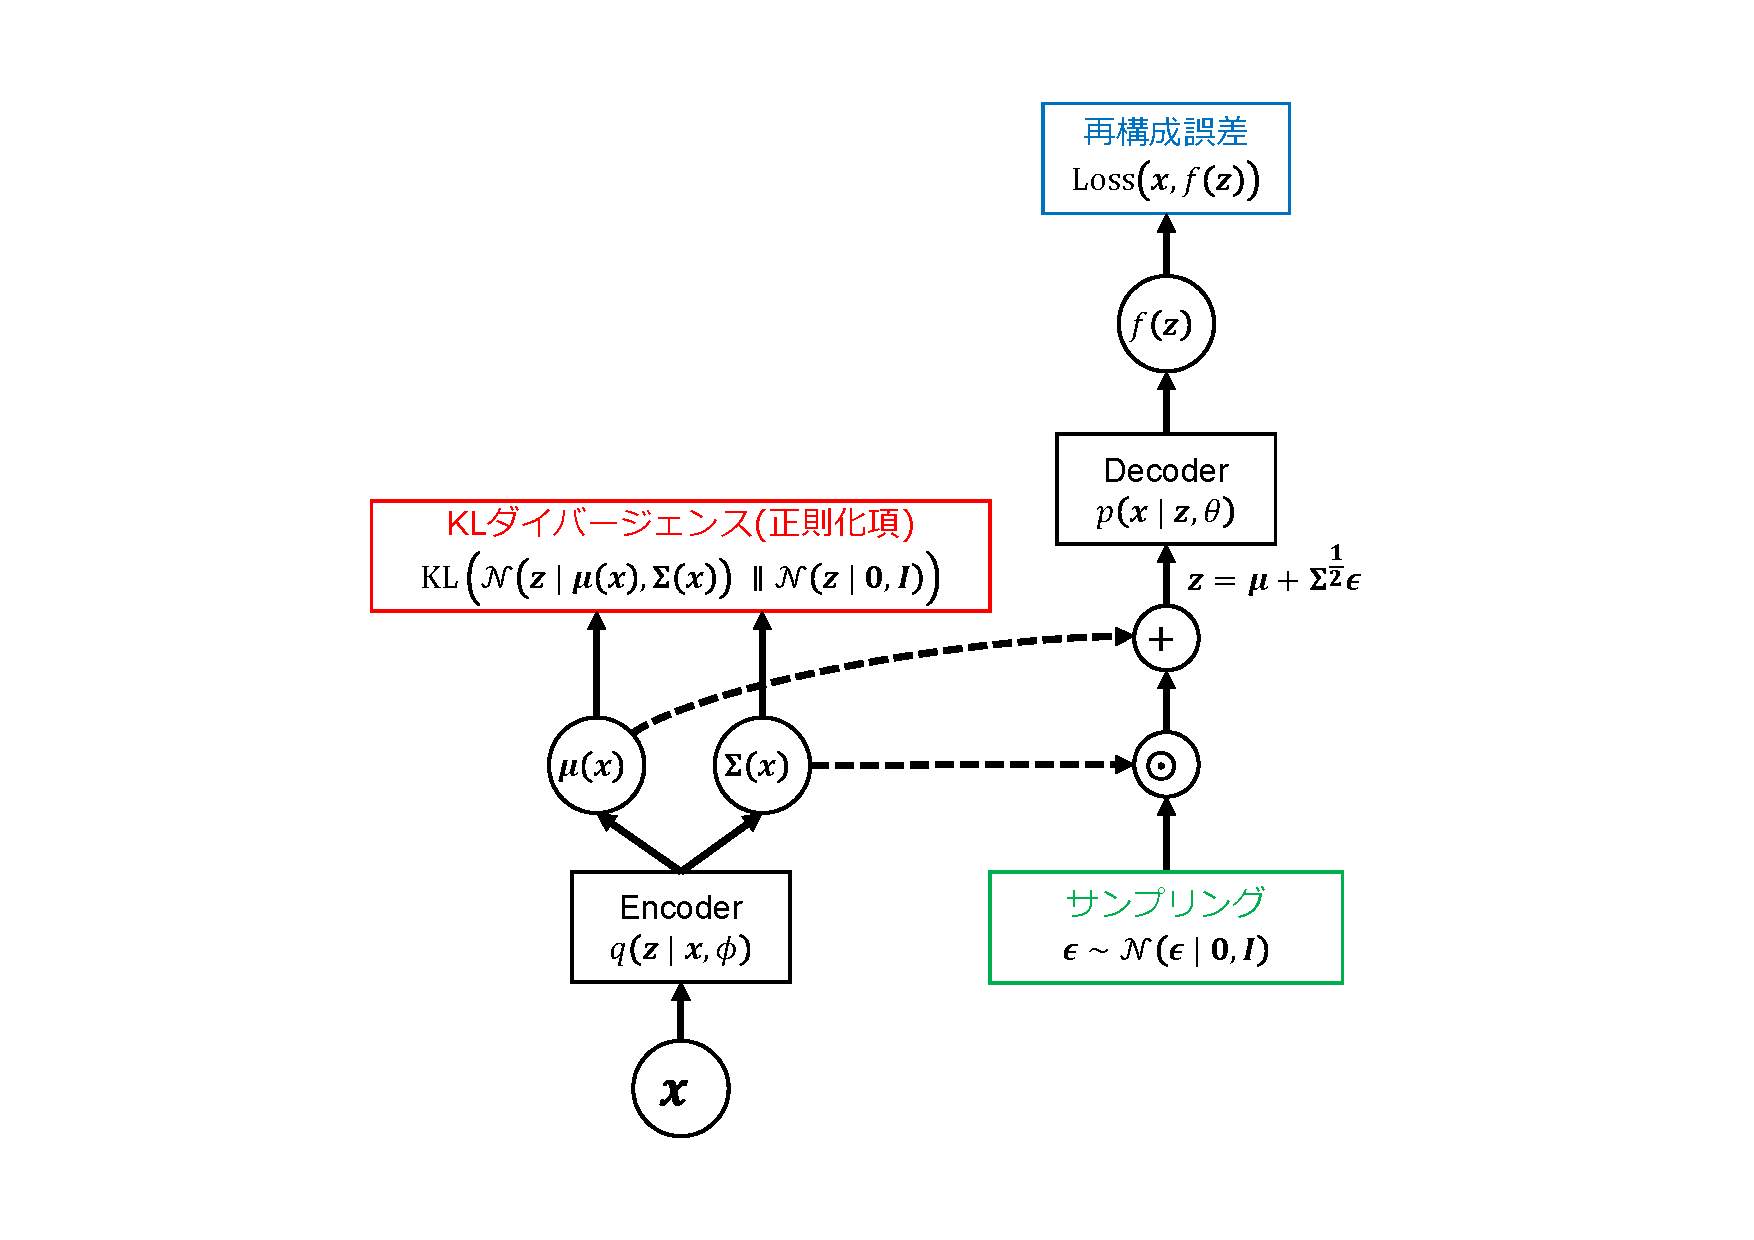
\includegraphics[keepaspectratio,scale=0.3,clip,trim=3cm 1cm 3cm 1cm]{vae-actual-architecture.pdf}
	\caption{VAEの構造}
	\label{fig:vae-actual-architecture}
\end{figure}

\end{frame}

\end{document}


\end{document}
